% !TeX root = main.tex
% !TeX spellcheck = en_US
% !TeX encoding = UTF-8

% This document typesets the Ph.D. dissertation of 
% David T. Wang, MIT/WHOI Joint Program, June 2017.
% 
% Document compiled with pdfLaTeX + BibLaTeX/Biber 
% from the TeX Live 2016 distribution on Windows 7.

\documentclass[11pt,twoside,final]{memoir} 	% draft, ms, final
%	\nonzeroparskip
	
\usepackage{etoolbox}

%Chemistry
\usepackage[version=4]{mhchem}
%\mhchemoptions{textfontcommand=\libertineLF}
%\usepackage{chemformula}

%Page setup
%\usepackage[letterpaper, top=1.45in, bottom=1.0in, left=1.0in, right=1.0in, showframe=false]{geometry}
%\usepackage[letterpaper, top=1.4in, bottom=1.2in, left=1.1in, right=1.1in, showframe=false]{geometry}
\usepackage[letterpaper, top=1.2in, bottom=1.0in, left=1.05in, right=1.05in, showframe=false]{geometry}
%\addtolength{\footskip}{1	ex} 

\usepackage{lscape}		% lscape rotates stuff in environment {landscape}, pdflscape rotates the page too
\usepackage{multicol} \setlength{\columnsep}{10pt}

\makepagestyle{myruled}
	\makeheadrule {myruled}{\textwidth}{\normalrulethickness}
%	\makefootrule {myruled}{\textwidth}{\normalrulethickness}{\footruleskip}
%	\makefootrule{myruled}{\textwidth}{\normalrulethickness}{1ex}
	\makeheadfootruleprefix{myruled}{\vspace*{3pt}}{}
	\makeevenhead {myruled}{\small\scshape\leftmark}{} {}
	\makeoddhead {myruled}{}{}{\small\itshape\rightmark}
	\makeevenfoot {myruled}{}{\figureversion{osf}\small\swshape \thepage} {}
	\makeoddfoot {myruled}{}{\figureversion{osf}\small\swshape \thepage} {}
	\makeatletter % because of \@chapapp
	\makepsmarks {myruled}{
		\nouppercaseheads
		\createmark {chapter} {both} {shownumber}{\@chapapp\ }{. \ }
		\createmark {section} {right}{shownumber}{} {. \ }
		\createmark {subsection} {right}{shownumber}{} {. \ }
%		\createmark {subsubsection}{right}{shownumber}{} {. \ }
		\createplainmark {toc} {both} {\contentsname}
		\createplainmark {lof} {both} {\listfigurename}
		\createplainmark {lot} {both} {\listtablename}
		\createplainmark {bib} {both} {\bibname}
		\createplainmark {index} {both} {\indexname}
		\createplainmark {glossary} {both} {\glossaryname}
	}
	\makeatother
%	\setsecnumdepth{subsubsection}
	\pagestyle{myruled}

%\pagestyle{ruled}
	\makeevenfoot {plain}{}{\figureversion{osf}\small\swshape \thepage} {}
	\makeoddfoot {plain}{}{\figureversion{osf}\small\swshape \thepage} {}
%\sloppybottom



%Font
\usepackage[LGR,T1]{fontenc}   
\usepackage[utf8]{inputenc}    % Load inputenc after fontenc.  https://tex.stackexchange.com/a/34046
\usepackage{textgreek}
%\usepackage{arev}
\usepackage[lf,mathtabular,minionint]{MinionPro}
%\usepackage[lf,proportional]{libertine}
\usepackage{gensymb}
\renewcommand*{\sfdefault}{phv}
\usepackage[lf]{MyriadPro}
\usepackage[scale=0.9]{inconsolata}

%Typography
\usepackage{microtype}
\input{glyphtounicode}	% fix ligatures ff, ffi, etc.
	\pdfgentounicode=1
\usepackage[super]{nth}
\usepackage[alsoload=synchem]{siunitx}
	\sisetup{detect-all}
\usepackage{enumitem}
	\setlist{nosep} % or \setlist{noitemsep} to leave space around whole list
\usepackage[hang,flushmargin,multiple]{footmisc}  %turned off [symbol*] option, decided to go with alphabetic (\alph) footnote markers, better compatibility with sans %turned off [para] option, incompatible with multicol
	\setlength\footnotemargin{1ex} %necessary, because otherwise, footnote indentation will be affected by width of footnote marker (e.g. "w" vs "i")
%	\renewcommand*{\footnotelayout}{\footnotesize\sffamily} %makes footnotes sans serif
%\usepackage[fragile]{bigfoot}
%  \DeclareNewFootnote[para]{default}

%% unnumbered footnotes
	\newcommand\blfootnote[1]{%
	\begingroup
	\renewcommand\thefootnote{}\footnote{#1}%
	\addtocounter{footnote}{-1}%
	\endgroup
}

%MISCELLANEOUS
\usepackage{verbatim}
\usepackage{lipsum}
\usepackage{xcolor, color, calc}
\providecommand\phantomsection{}
\usepackage{pdfpages}

%Math
\usepackage{nicefrac}
\usepackage{widetext}% needs packages "flushend" & "cuted" of "sttools"
% bundle, which perhaps must separately be installed
%http://tex.stackexchange.com/a/151507 - How to typeset wide equation spannuing 2col
\usepackage{xfrac}
\usepackage{amsmath,amssymb}


%Tables
\usepackage{rotating}
\usepackage{dcolumn} 
	\newcolumntype{d}[1]{D{.}{.}{#1}}
\usepackage{longtable} 	% typesetting longtables may require three or more passes through pdflatex
\usepackage{booktabs}
\usepackage[toc,eqno,enum,bib,lineno]{tabfigures}
\usepackage{multirow}
\AtBeginEnvironment{tabular}{%
	\figureversion{lf,tab} 
}
\AtBeginEnvironment{longtable}{%
	\figureversion{lf,tab} 
}
\usepackage[font=small]{caption} 
	\DeclareCaptionLabelFormat{bold}{\bfseries #1~#2}
	\DeclareCaptionLabelSeparator{bar}{\:\:|\:\:}
	\captionsetup{labelformat=bold,labelsep=bar}
	\DeclareCaptionFormat{myformat}{#1#2#3\hrulefill}
	\DeclareCaptionFormat{myregular}{#1#2#3}
	\DeclareCaptionFormat{myruletop}{\hrule\protect\\\vspace{10pt} #1#2#3}
	\captionsetup[SCfigure]{format=myformat}		% hrule below caption for SCfigures
\usepackage[flushleft]{threeparttable}	% for footnotes https://tex.stackexchange.com/a/327385, https://tex.stackexchange.com/a/57170
\usepackage{threeparttablex}
	\makeatletter 
	\g@addto@macro\TPT@defaults{\small} 
	\makeatother
\let\oldtabular\tabular 
	\renewcommand{\tabular}{\small\oldtabular}
\let\oldtabularx\tabularx 
	\renewcommand{\tabularx}{\small\oldtabularx}
\let\oldlongtable\longtable
	\renewcommand{\longtable}{\small\oldlongtable}

%Figures
%\usepackage[toc,eqno,enum,bib,lineno]{tabfigures}  %% MODIFIED ADDED to use tabular figures in other places (besides tables; recall, must do: \figureversion{tabular} before every table! otherwise lining figures would be used)
\usepackage{graphicx,grffile}
\usepackage{epstopdf}
\usepackage{sidecap}
	\renewcommand{\sidecaptionrelwidth}{0.85}
	\renewcommand{\sidecaptionsep}{4ex}

%Sectioning
\setcounter{tocdepth}{2}
\setcounter{secnumdepth}{3}
\setsecnumdepth{subsubsection}
%\usepackage{chngcntr}
%	\counterwithin*{section}{chapter}
\usepackage{titlesec}
%	\titleformat{\chapter}
%		{\Large\bfseries} % format
%		{\huge\thechapter}                % label
%		{20pt}             % sep
%		{\huge}           % before-code
	\titleformat{\section}{\normalsize\bfseries\sffamily}{\thesection}{1em}{\MakeUppercase} 
	\titleformat*{\subsection}{\normalsize\bfseries\sffamily}
	\titleformat*{\subsubsection}{\small\bfseries\itshape\sffamily \color{black} 
		%\fontfamily{lmss}\selectfont
		}
\setbeforeparaskip{1.5ex plus 1ex minus .2ex}
\setparaheadstyle{\itshape\raggedright}
\aliaspagestyle{cleared}{chapter}
%\chapterstyle{pedersen} 
%\titleformat{\chapter}[hang]{\Huge\bfseries}{\thechapter\hsp\textcolor{gray75}{|}\hsp}{0pt}{\Huge\bfseries}
\makeatletter
\makechapterstyle{combined}{
%	\setlength{\midchapskip}{-60pt}
%	\setlength{\afterchapskip}{2.5cm}
	\renewcommand\afterchapternum{\par\nobreak\vskip -26pt}
	\renewcommand*{\printchaptername}{}
	\renewcommand*{\chapnumfont}{\normalfont\bfseries\fontsize{80}{0}\selectfont}

	\renewcommand*{\printchapternum}{\flushright\chapnumfont\textcolor[rgb]{.647,.129,.149}{\raisebox{2cm}[0pt][0pt]{\smash{{\Large\scshape \@chapapp\;\;}\thechapter}}}}

	\renewcommand*{\chaptitlefont}{\normalfont\huge\itshape}
	\renewcommand*{\printchaptertitle}[1]{%
		\raggedright\chaptitlefont\parbox[t]{\textwidth-0cm}{%
			\microtypesetup{protrusion=false}%
			\raggedright##1}}
}
\makeatother
\chapterstyle{combined}
%\chapterstyle{lyhne}
%\headstyles{wilsondob}

\usepackage{abstract}
%	\renewcommand{\abstractname}{\normalfont\sffamily\footnotesize \textperiodcentered\;\textperiodcentered\;\textperiodcentered\;\textperiodcentered\;\textperiodcentered\quad\!\! ABSTRACT } 
	\renewcommand{\abstractname}{\normalfont\sffamily\footnotesize ABSTRACT } 
%	\renewcommand{\absnamepos}{flushleft}
	\renewcommand{\absnamepos}{center}
	
\aliaspagestyle{afterpart}{plain}	% put pagenum on even page following appendixpage*
	
%Bibliography
%\usepackage[style=science,backend=bibtex8,article-title=true]{biblatex}
%\bibliography{thesis.bib}
%\usepackage[style=authoryear, backend=bibtex, maxcitenames=2, maxbibnames=99, natbib=true, firstinits=true, isbn=false, url=false, doi=false, eprint=false]{biblatex}
%\bibliography{thesis.bib}
%\renewbibmacro{in:}{%
%	\ifentrytype{article}{}{%
%		\printtext{\bibstring{in}\intitlepunct}}}
\usepackage[style=authoryear,%-icomp,% articletitle=true,
			backend=biber,		% biber handles sorting much better
			uniquename=false, 	% If two different authors have the same surname, biblatex adds the first name to identify each of them.  This turns that behavior off.
			uniquelist=false,	% https://tex.stackexchange.com/a/69030
%			defernumbers,
%			bibstyle=numeric,
%			bibencoding=utf8,	% for Chinese characterers
%			natbib=true,
			sorting=ynt]{biblatex}
\setlength\bibitemsep{0.2\baselineskip}
\assignrefcontextentries[]{*}
\bibliography{thesis.bib}
\renewbibmacro{in:}{%
	\ifentrytype{article}{}{%
		\printtext{\bibstring{in}\intitlepunct}}}
\DeclareFieldFormat*{citetitle}{#1} 	% remove quotes around citetitle
\DeclareFieldFormat*{citeyear}{{\bfseries #1}}

%\appto\bibsetup{\let\x\chinesechar}
%\newcommand\chinesechar[1]{\includegraphics[height=\fontcharht\font`T]{pia#1}}

%Cross-links
\definecolor{myred}{rgb}{.647,.129,.149} 
\usepackage[pdfencoding=auto, 
			psdextra, 
			bookmarksnumbered, 
			colorlinks=true, 
			linktocpage=true,
			allcolors=myred,
			urlcolor=cyan]{hyperref}
\hypersetup{pdfauthor={David T. Wang},
	pdftitle={The Geochemistry of Methane Isotopologues},
	pdfsubject={Ph.D. thesis, MIT/WHOI Joint Program, June 2017},
	pdfkeywords={methane biogeochemistry, clumped isotopes, hydrogen exchange}}
\usepackage{memhfixc}
\def\equationautorefname{Eqn.}
\def\figureautorefname{Fig.}
\def\chapterautorefname{Chapter}
\def\sectionautorefname{§}
\def\subsectionautorefname{§}
\def\subsubsectionautorefname{§}

\makeatletter	% Fixes an issue with starred section* and hyperref for \nameref, https://tex.stackexchange.com/a/123667/23509.  May require multiple (~5?) runs of pdflatex to make it work.
\def\ttl@useclass#1#2{%
	\@ifstar
	{\ttl@labeltrue\@dblarg{#1{#2}}}% {\ttl@labelfalse#1{#2}[]}%
	{\ttl@labeltrue\@dblarg{#1{#2}}}}
\makeatother

\newcommand{\mrefs}[3][]{\hyperref[#3]{#2~\ref*{#3}#1}}	% e.g., \mrefs{Eqns.}{eqn:4:15}, or \mrefs[b]{Fig.}{fig:4:2} = Fig.~4.2b



%Custom shortcuts
%% define \permille as the unicode default input, set OT1 within group
\newcommand{\permille}{\text{ ‰}} % \usefont automatically calls \selectfont; change to MinionPro-OsF to scale the permille symbol with OSF numbers; I'm using \text as a wrapper so that the command can be called in math mode directly, as well as in text mode.
%\newcommand{\iso}[1]{\ce{^{#1}{S}}}
%\newcommand{\eps}{$^{34}\varepsilon$}
\newcommand{\tss}[1]{\textsuperscript{#1}}

%DRAFTING
\usepackage{datetime}
%\includeonly{cover}
%\PassOptionsToPackage{demo}{graphicx}
\usepackage{lineno}
\usepackage[printwatermark=false]{xwatermark}
	\newwatermark[firstpage,lastpage,color=red!15,angle=45,scale=3,xpos=0,ypos=0]{DRAFT \protect\\ \scriptsize \yyyymmdddate\today\ :: \currenttime} 	% allpages, lastpage
\usepackage{afterpage}	% allows lscape to float around, https://tex.stackexchange.com/a/262240/23509, https://tex.stackexchange.com/q/115112/23509
%\usepackage{libertine}
%\interfootnotelinepenalty=10000 	% inhibit splitting of footnotes, doesn't seem to work for Chap 3 footnotes
%\usepackage{fnbreak}


\begin{document}
	
%	\linenumbers
	
	\frontmatter*	
	
%	\thispagestyle{empty}


\vspace*{1in}

{
%	\fontfamily{jkpk}\selectfont
%\fontfamily{gentium}\selectfont
{\noindent\Large\  \color{myred} \uppercase{the geochemistry of methane isotopologues}}


\vspace{1in}



%\sffamily
{\bfseries David Texan Wang}\\

B.S., California State University, Los Angeles, 2011\\

Submitted in partial fulfillment of the requirements for the degree of

Doctor of Philosophy

at the

MASSACHUSETTS INSTITUTE OF TECHNOLOGY

and the

WOODS HOLE OCEANOGRAPHIC INSTITUTION


}







\begin{comment}

The geochemistry of methane isotopologues

by

David Texan Wang

B.S., California State University, Los Angeles, 2011

Submitted in partial fulfillment of the requirements for the degree of

Doctor of Philosophy

at the

MASSACHUSETTS INSTITUTE OF TECHNOLOGY

and the

WOODS HOLE OCEANOGRAPHIC INSTITUTION

June 2017

© 2017, \emph{David T. Wang}\\
All rights reserved.

The author hereby grants MIT and WHOI permission to reproduce and to
distribute publicly paper and electronic copies of this thesis document
in whole or in part in any medium now known or hereafter created.

\emph{Author: \_\_\_\_}

Department of Earth, Atmospheric and Planetary Sciences, MIT \&

Marine Chemistry and Geochemistry Department, WHOI

MIT/WHOI Joint Program in Oceanography/Applied Ocean Science and
Engineering

MONTH DAY, 2017

\emph{Certified by: }

Shuhei Ono

Associate Professor of Geochemistry, MIT

Thesis Supervisor

\emph{Accepted by: }

Shuhei Ono

Chair, Joint Committee for Chemical Oceanography


\end{comment}

	\includepdf[pagecommand={\thispagestyle{empty}},
	pages=1]{makecover.pdf}
	
	\includepdf[pagecommand={\thispagestyle{plain}},
	pages=2-3]{makecover.pdf}
	
	\cleardoublepage
	
%	\title{The geochemistry of methane isotopologues}
%	\author{David Texan Wang\thanks{MIT/WHOI Joint Program}}
%	\date{May \nth{4}, 2017}
%	
%	\begin{titlingpage*}
%		\aliaspagestyle{titlingpage}{plain}
%		\setlength{\droptitle}{30pt}
%		\maketitle
%		\begin{abstract}
This thesis documents the origin, distribution, and fate of methane and
several of its isotopic forms on Earth.~~Using observational,
experimental, and theoretical approaches, I illustrate how the relative
abundances
of~\textsuperscript{12}CH\textsubscript{4},~\textsuperscript{13}CH\textsubscript{4},~\textsuperscript{12}CH\textsubscript{3}D,
and \textsuperscript{13}CH\textsubscript{3}D record the formation,
transport, and breakdown of methane in selected settings.

\qquad Chapter~2 reports precise determinations
of~\textsuperscript{13}CH\textsubscript{3}D, a ``clumped'' isotopologue
of methane, in samples collected from various settings representing many
of the major sources and reservoirs of methane on Earth.~~The results
show that the information encoded by the abundance
of~\textsuperscript{13}CH\textsubscript{3}D enables differentiation of
methane generated by microbial, thermogenic, and abiogenic processes.~~A
strong correlation between clumped- and hydrogen-isotope signatures in
microbial methane is identified and quantitatively linked to the
availability of H\textsubscript{2}~and the reversibility of
microbially-mediated methanogenesis in the environment.~~Determination
of~\textsuperscript{13}CH\textsubscript{3}D in combination with
hydrogen-isotope ratios of methane and water provides a sensitive
indicator of the extent of C--H bond equilibration, enables
fingerprinting of methane-generating mechanisms, and in some cases,
supplies direct constraints for locating the waters from which migrated
gases were sourced.~~Chapter~3 applies this concept to constrain the
origin of methane in hydrothermal fluids from sediment-poor vent fields
hosted in mafic and ultramafic rocks on slow- and ultraslow-spreading
mid-ocean ridges.~~The data support a hypogene model whereby methane
forms abiotically within plutonic rocks of the oceanic crust at
temperatures above ca.\ 300~$^{\circ}$C during respeciation of magmatic
volatiles, and is subsequently extracted during active, convective
hydrothermal circulation.~~Chapter~4 presents the results of culture
experiments in which methane is oxidized in the presence of
O\textsubscript{2}~by the bacterium~\emph{Methylococcus
	capsulatus}~strain Bath.~~The results show that the clumped isotopologue
abundances of partially-oxidized methane can be predicted from knowledge
of~\textsuperscript{13}C/\textsuperscript{12}C and D/H isotope
fractionation factors alone.~~

\end{abstract}
%	\end{titlingpage*}
	
	%Column Separation
%	\setlength{\columnsep}{2\columnsep}
	
%	\cleardoublepage
%	\currentpdfbookmark{Table of Contents}{Table of Contents}
	%\addcontentsline{toc}{chapter}{Contents}
	\tableofcontents
	\cleardoublepage
%	\currentpdfbookmark{List of Figures}{List of Figures}
	%\addcontentsline{toc}{chapter}{List of Figures}
	\listoffigures
	\cleardoublepage
%	\currentpdfbookmark{List of Tables}{List of Tables}
	\listoftables
	%\addcontentsline{toc}{chapter}{List of Tables}
	
	\chapter*{Acknowledgments}
\chaptermark{Acknowledgments}
\addcontentsline{toc}{chapter}{Acknowledgments}

I fear that this section will not do justice to the people I have not
the space to thank individually. Alas, here goes. To those whose names
are not specifically listed here, thank you too.

I wish first to thank Shuhei Ono. The work this thesis represents could
not have happened without his bold vision and the license to explore and
question that working in his lab afforded. His unbridled optimism,
breadth of scientific curiosity, personal integrity, and accessibility
to his personnel are traits I one day hope to emulate. I thank him for
his nonjudgmental yet appropriately measured support of many of my
ideas---even those that led nowhere---, for believing in me even when I
found it difficult to do so myself, and for teaching me to change pump
oil, build vacuum lines, and drink Icelandic vodka.

I also wish to thank my thesis committee members Jeff Seewald, Roger
Summons, and John Pohlman, for their input and genuine interest in my
projects, for their coauthorship on one or more manuscripts, and for
serving as sounding boards for questions about life and career.  Meg Tivey is thanked for chairing my defense
and for her comments on this thesis.

Many members of the Ono lab have contributed time or ideas towards the
work in this thesis. I particularly wish to acknowledge Danielle Gruen,
who has been a wonderful friend, stand-in sibling, and multi-talented
colleague. Without her efforts in the field and the lab, we would not
have made the discovery of the ``hot cow'' that is now perhaps the MIT
Hardcore Stable Isotope Laboratory's best-known result. Bill Olszewski
has been a fount of technical wizardry and occasional oddball humor,
both of which are appreciated. Eoghan Reeves, Genming Luo, Andrew
Whitehill, Shikma Zaarur, Yenny Gonzales Ramos, and Jeemin Rhim are
thanked for their company both at and away from the shop.

Other members of the E25-6\textsuperscript{th} floor community have made
it worth coming into work each day. These include my officemates Ana de
Santiago Torio, Gilad Antler, Mirna Daye, and Kristin Woycheese, and
reliable sources of conversation Simone, Sharon, Christine, Xiaolei, Ross, Shane, Emily, Robert, Haitao, Annie, Christopher, Ainara, and Melody. My fellow JP students---including Ning, Nick, Kate, Evan, Rene, and Craig---provided much needed inspiration (and commiseration and distraction) at times. 

I have had the privilege of working in several other labs during the
past six years.  Tanja Bosak served as my co-advisor for my Generals
project on sulfate reducing bacteria. I thank her for welcoming me into
her lab, for helping me become a more succinct writer and shrewd reader, and
for her encouragement at a particularly frustrating point in my
research. I also thank Mak Saito, who took me under his wing my first
year, offered the opportunity to join my first oceanographic cruise (and
first equator-crossing!), and---after I splashed some acid on myself
while hastily preparing reagents before departing for said
cruise---kindly drove me to his house so that I could have a shower, a
change of clothes, and a day-old scone.  I thank Jeff Seewald for making me feel welcome in his group while I
puttered about trying to deuterate his lab.  

Many thanks are due to members of the Bosak, Saito, and Seewald labs. Min Sub Sim
showed me how to work with sulfate-reducing bacteria, and Peter Hedman,
Alex Evans, and Laura Meredith provided assistance at one time or
another during my first two years at MIT. Help or advice from Sean Sylva, Jill McDermott,
Dawn Moran, Matt McIlvin, Tyler Goepfert, and others in the Fye and 
Watson Buildings at WHOI are gratefully acknowledged.

Several other faculty members dispensed much needed advice at one point
or another, including Ed Boyle, Scott Wankel, Dave Glover, Amanda
Spivak, Scott Doney, Carl Lamborg, and Frieder Klein. Bernhard Peucker-Ehrenbrink, Liz Kujawinski,
and Mark Kurz assisted in navigating the administrative waters of the
JP.\@ Rachel Stanley kindly served as chair for my thesis proposal
defense. I thank those instructors in whose courses I did not
actually enroll, but who still allowed me to participate in their study
tours---David McGee, Taylor Perron, and Oli Jagoutz (MIT),
Rob Sohn, Meg Tivey \& Andrew Daly (Geodynamics 2015, WHOI), John Shaw
(Harvard), and Grant Garven (Tufts).

The administrators in E25, particularly Melody Abedinejad, Mary Eliff,
and (briefly) Annora Borden, are thanked for making life easier in too
many ways to name. I also thank the staff of the MIT Joint Program
Office (Ronni Schwartz and Kris Kipp), PAOC administration (Christine
Maglio), ERL administration (Anna Shaughnessy and Josh Kastorf), EAPS HQ
(esp. Roberta Allard, Angela Ellis, Brian Smith, and Mark Pendleton),
the WHOI MC\&G Department (esp.\ Mary Zawoysky), and the Academic
Programs Office (Julia Westwater, Lea Fraser, Tricia Morin Gebbie,
Christine Charette, Valerie Caron, Meg Tivey, and Jim Yoder). Also, I
want to acknowledge the security staff at WHOI---they more than once let
me into a locked building or gave me a lift back to Winding Lane---, as
well as the custodial staff at MIT, particularly Sergio Medina, who I
could always count on to share stories and snacks when working late into
the night.

I have been lucky enough to be plugged into several wonderful scientific
communities outside of MIT and WHOI, thanks in no small part to Shuhei
and several collaborators. Thanks goes to the instructors and students
of the International Geobiology Summer Course 2013 (it didn't suck!) for
exposing me to the geobiological sciences, and the Agouron Institute and
the Henry Houghton fund of PAOC for sponsoring my participation. The
Deep Carbon Observatory (DCO) funded much of the work in this thesis,
and also afforded me the opportunity to attend and present at several
meetings; Craig Schiffries, Mitch Sogin, Barbara Sherwood Lollar,
Kai-Uwe Hinrichs, and Fumio Inagaki, among others, are thanked for these
opportunities. Two other much-needed breaks punctuated my graduate
studies. I thank Jen Shosa, Michael Lawson, Mike Formolo, Glenn
Hieshima, and everyone else who made being an intern at ExxonMobil
interesting and fun. I also thank my entire IODP Expedition 370
``T-Limit'' family, particularly Verena Heuer, Fumio Inagaki, Akira
Ijiri, Flo Schubotz, Hayley Manners, Masanori Kaneko, Bernhard
Viehweger, and Art Spivack for a great few months at sea and in Kochi.

Miscellaneous thanks goes to the folks at Aerodyne Research (Dave
Nelson, Barry McManus, Joanne Shorter, Mark Zahniser, Christoph Dyroff,
and Stanley Huang) for technical support, Issaku Kohl for organizing the
return of a stranded sample, L.~Taras Bryndzia for arranging funding
from Shell through the Society of Energy Fellows at MIT to support my
last year of studies, Chris Clayton for sharing unpublished data which
helped frame my views on the origin of H in thermogenic hydrocarbons,
Carolyn Ruppel for connecting me to the gas hydrates world,
Jeff Dick for technical support related to CHNOSZ,
Jordan Bird for sampling a rice paddy, my previous research mentors 
(Andre Ellis, Oliver Dorigo, and Chintda Santiskulvong) for introducing me to science,
Penny Morrill for telling me something I needed to hear,
and Lisa Morgan Morzel for gifting me her DCO hat.

My friends outside of EAPS and the JP have played no insignificant role
in helping me maintain perspective on life. For this, I thank my
roommates past and present (esp.\ Nate, Diego, and Benedikt), sailing
partner (Pablo), friends from Harvard EPS (Yanpeng and Joe), fellow
Boston-area EEP alumni (including David, Alex, Daniel, and Matt), and
friends from the MIT Concert Band (Melissa, Tom~C., Brynna, Faith, and
many others). Tom Reynolds deserves a special mention; his work ethic
and constant encouragement as conductor has made me a much improved
trumpet player over my almost five years with the band.

Finally, I thank my parents. They have been voices of encouragement and
reason during my happiest days and my darkest. This doctoral thesis
completes what they came to the U.S. decades ago to begin, but
ultimately chose not to finish so that their son might have a better
shot at doing so himself.

\clearpage

\section{Financial support}

The research activities documented in this thesis were made possible by
grants to my advisor from the U.S. National Science Foundation
(NSF award EAR-1250394), the
National Aeronautics and Space Administration (NASA) Astrobiology
Institute (NAI, University of Colorado, Boulder, CAN 7 under
Cooperative Agreement NNA15BB02A), the Department of Energy (DOE, Small Business Innovation Research program, contract DE-SC0004575),
the Alfred P. Sloan Foundation via the Deep Carbon Observatory, and a
Shell Graduate Fellowship through the MIT Energy Initiative.

I completed the bulk of the work in this thesis while being supported by
a National Defense Science and Engineering Graduate (NDSEG) Fellowship
awarded through the Office of Naval Research of the U.S. Department of
Defense. The Stanley W. Watson Fellowship Fund provided support during
my first summer term at WHOI. The Charles M. Vest Presidential
Fellowship at MIT supported me in the first year of my Ph.D. studies. I
received additional support that year through NSF award EAR-1159318
(to S. Ono and T. Bosak) and the Walter \& Adel Hohenstein
Graduate Fellowship of Phi Kappa Phi.  The MIT Earth Resources Laboratory 
and PAOC Houghton Fund funded my attendance at several conferences.
	
	\cleardoublepage
	\mainmatter*
	\chapter{Introduction}\label{ch:1}

\begin{sidewaysfigure}
	\centering
	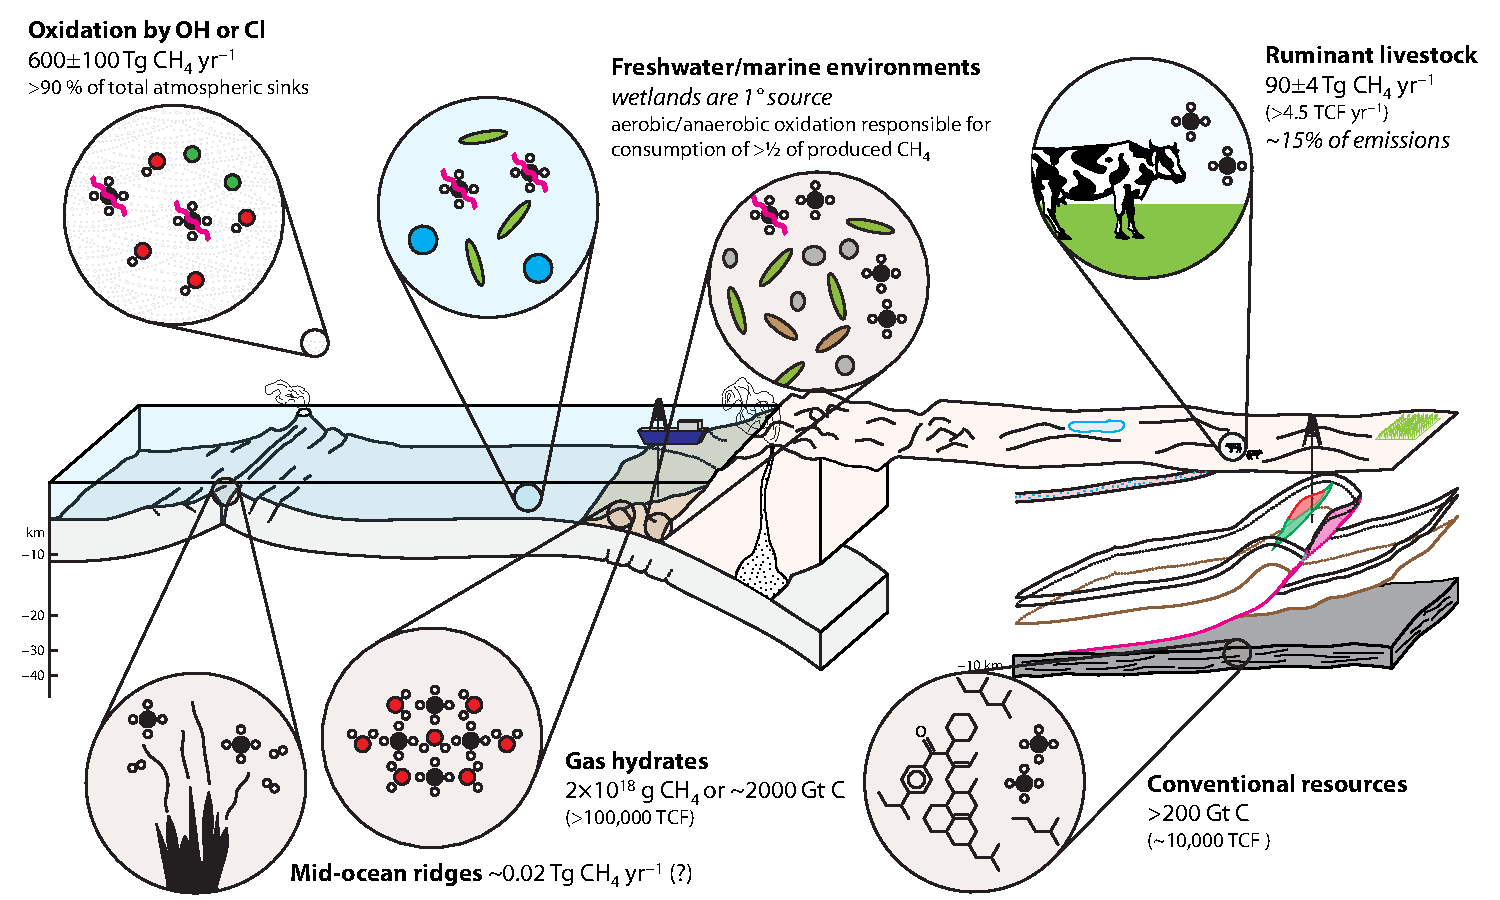
\includegraphics[width=0.95\textwidth]{figures/Fig1.1.pdf}
	\caption[Reservoirs and fluxes of CH\textsubscript{4} on Earth]{Some of the many reservoirs and fluxes of methane on
		Earth, and their relative magnitudes \parencite{Kvenvolden_1988_CG,Keir_2010_GRL,IPCC_AR5_WG1,Kirschke++_2013_NG}.}
	\label{fig:1:1}
\end{sidewaysfigure}

Methane is the simplest and most abundant hydrocarbon. \mrefs[]{Figure}{fig:1:1} shows some statistics on the
portions of the methane cycle that this thesis touches upon.

\section{Essential definitions}\label{sec:1:essential-definitions}


\begin{SCfigure*}
	\centering
	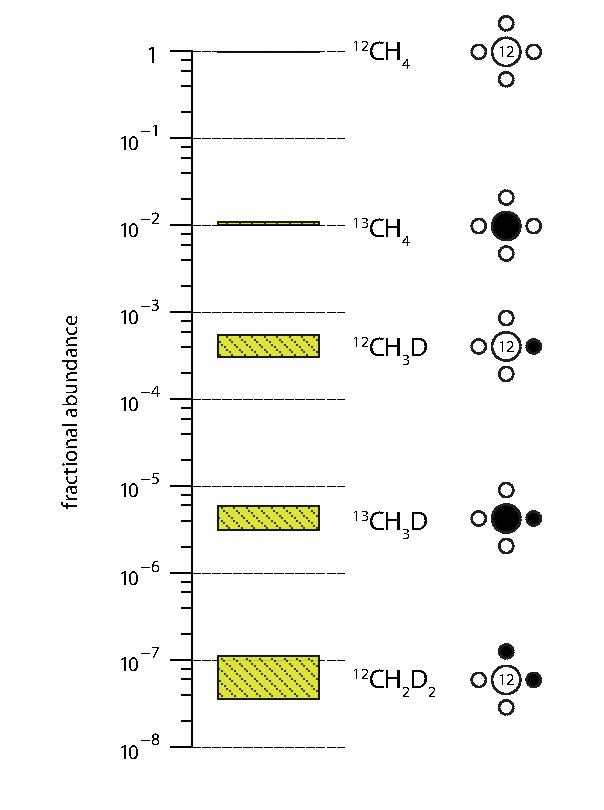
\includegraphics[width=0.52\textwidth]{figures/Fig1.2.pdf}
	\captionsetup{format=myformat}	% hrule beneath caption
	\caption[Natural abundances of methane isotopologues]{Relative abundance of the five most abundant methane
		isotopologues in nature.\protect\\}
	\label{fig:1:2}
\end{SCfigure*}


The \emph{isotopologues} (or isotopic homologues) of a compound have the
same elemental composition and chemical structure, but differ only in
the identity of the isotopes of one or more atoms. The word
\emph{isotopologue} is also seen as \emph{isotopolog}.

\sidecaptionvpos{figure}{t}	%typset sidecap at top
\begin{SCfigure*}
	\centering
	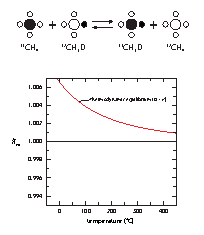
\includegraphics[width=0.52\textwidth]{figures/Fig1.3.pdf}
	\captionsetup{format=myregular}	% no hrule beneath caption
	\caption[Equilibrium constant for \textsuperscript{13}CH\textsubscript{3}D formation vs.\ temperature]{Temperature-dependence of the equilibrium constant for the
		isotopologue exchange reaction in \mrefs[]{Reaction}{eqn:1:exchange} (also shown graphically at
		top).}
	\label{fig:1:3}
\end{SCfigure*}
\sidecaptionvpos{figure}{b}	%reset to default


\begin{figure}
	\centering
	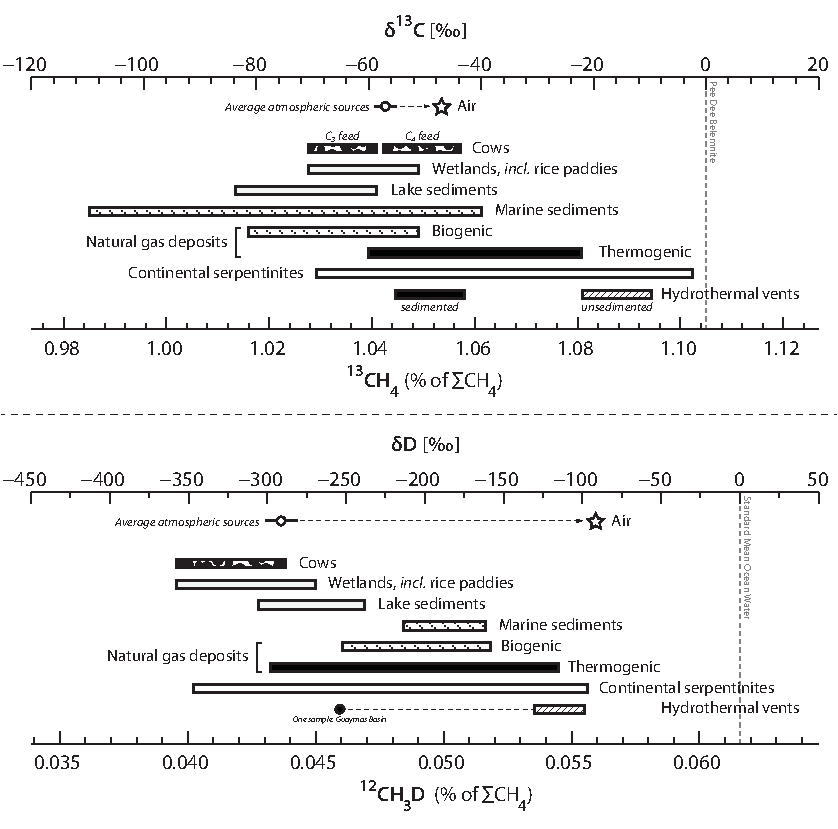
\includegraphics[width=0.75\textwidth]{figures/Fig1.NA.pdf}
	\captionsetup{format=myformat}	% hrule beneath caption
	\caption[Natural abundances of singly-substituted methane isotopologues]{Typical abundances of \textsuperscript{13}CH\textsubscript{4} (\textit{top}) and \textsuperscript{12}CH\textsubscript{3}D (\textit{bottom}) in nature.}
	\label{fig:1:NA}
\end{figure}


The goal of this thesis is to help map the distribution and behavior of
the four most abundant methane isotopologues at the Earth surface and in
the crustal subsurface. These isotopologues are shown in \mrefs[]{Figs.}{fig:1:2} and~\ref{fig:1:3} (approximate ranges of abundance for the singly-substituted methane isotopologues are 
shown in \autoref{fig:1:NA}) and
written in the isotope exchange reaction below:
\begin{equation}\label{eqn:1:exchange}
{}^{13}\text{CH}_4+ {}^{12}{\text{CH}}_3\text{D}\rightleftharpoons {}^{13}{\text{CH}}_3\text{D}+ {}^{12}{\text{CH}}_4
\end{equation}


\begin{SCfigure*}
	\centering
	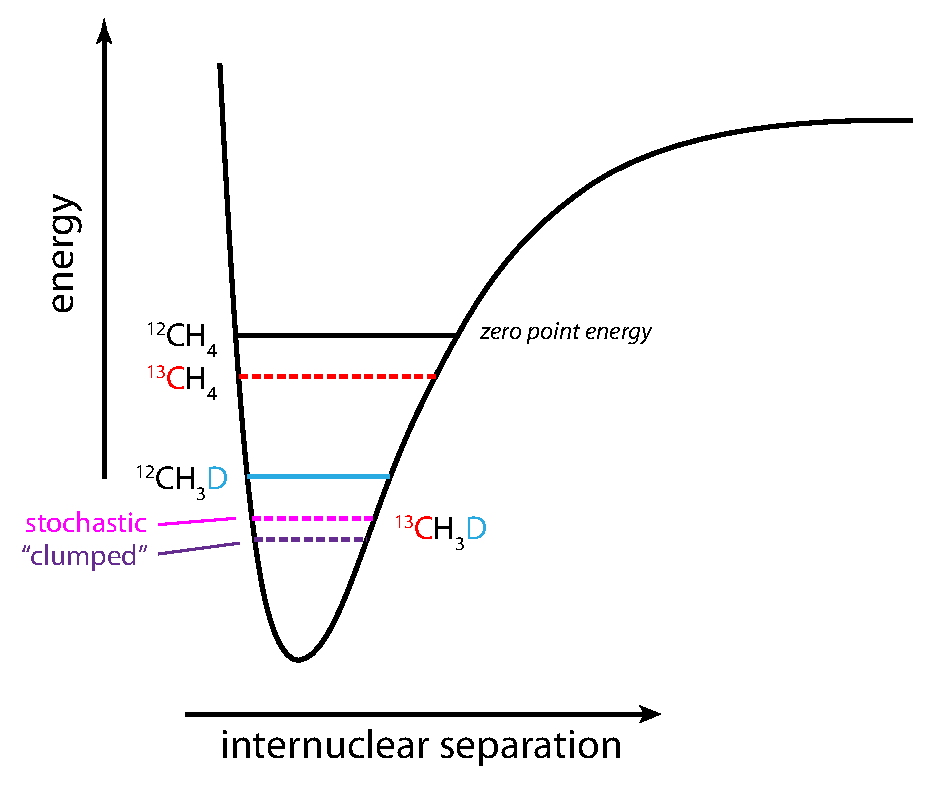
\includegraphics[width=0.55\textwidth]{figures/Fig1.4.pdf}
	\captionsetup{format=myformat}	% hrule beneath caption
	\caption[Statistical mechanical origin of preferential heavy-isotope clumping]{Zero-point energy lowering and the origin of non-stochastic clumped isotopologue composition
		at equilibrium.  The zero-point energy (the energy of the ground state, the quantum state with the lowest possible energy) of a molecule of methane is lowered upon substitution of heavy isotopes.  The amount by which the zero-point energy is lowered upon double-isotope substitution (e.g., \ce{^{12}CH4} to \ce{^{13}CH3D}) is slightly greater than the sum of the effects of substituting only one heavy isotope (to make \ce{^{13}CH4} and \ce{^{12}CH3D}).  This deviation from the ``rule of the geometric mean'' \parencite{Bigeleisen_1955_JCP} is particularly pronounced at lower temperatures, and is the origin of the preferential clumping at equilibrium shown in \autoref{fig:1:3}.  For a detailed treatment, readers are referred to \textcite{Eiler_2007_EPSL}.}
	\label{fig:1:4}
\end{SCfigure*}

In this reaction, one deuterium (D) is exchanged for one hydrogen (H),
while leaving in place the two different carbon (C) isotopes and the
three other H's to which each C is connected. The equilibrium constant
for this reaction is primarily a function of temperature (the
effect of pressure is negligible at near-surface conditions), and is
shown in \autoref{fig:1:3}. The equilibrium constant for this reaction
asymptotically approaches unity as temperatures increase towards
infinity. A sample of methane whose relative abundance of isotopologues
obey the relation
\cee{(\textsuperscript{13}CH\textsubscript{4})(\textsuperscript{12}CH\textsubscript{3}D)
=
(\textsuperscript{13}CH\textsubscript{3}D)(\textsuperscript{12}CH\textsubscript{4})}
(i.e., has a reaction quotient equal to unity) is said to have a
\emph{stochastic distribution} of isotopes among isotopologues. At
lower temperatures, the equilibrium constant is greater than one, albeit
only slightly, by 0.6\% or 6‰ (permil) at room temperature. The origin
of this \emph{clumpiness} at equilibrium at lower temperatures arises from a disproportionate lowering of zero-point energy upon clumping of two or more heavy isotopes (\autoref{fig:1:4}). For more on this topic, readers are referred to \textcite{Eiler_2007_EPSL}.



\begin{SCfigure*}
	\centering
	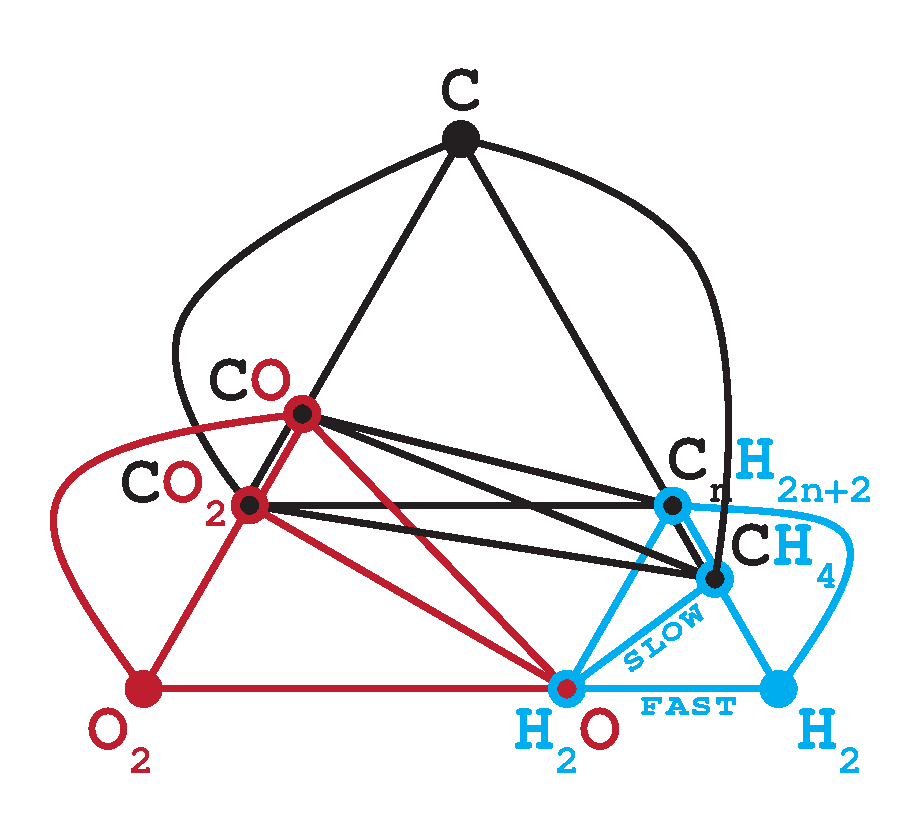
\includegraphics[width=0.4\textwidth]{figures/Fig1.5.pdf}
	\captionsetup{format=myformat}	% hrule beneath caption
	\caption[Pathways for isotopic exchange amongst C--O--H species]{Pathways for isotopic exchange between major species in
		the system C--O--H. The core \& ring of nodes with two colors represent
		the central \& outer atoms, respectively. Each line in this diagram
		represents a geothermometer comprising the isotope ratios of the
		corresponding element in the species at the nodes connected by the line. (Not shown:
		H\textsubscript{3}COOH, H\textsubscript{2}CO, CH\textsubscript{3}OH)}
	\label{fig:1:5}
\end{SCfigure*}

Attainment of equilibrium in CH\textsubscript{4} clumped isotopologue
abundances requires reordering of the C--H bonds within molecules. This
may occur by homogeneous (direct) exchange of H between two
CH\textsubscript{4} molecules, or by all CH\textsubscript{4} molecules
independently exchanging H with a second species (heterogeneous).
Understanding the mechanisms enabling exchange in various environments
is vital for correct interpretation of classical and novel stable
isotope geothermometers. \mrefs[]{Figure}{fig:1:5} shows the many pathways by which
several single-carbon compounds can exchange isotopes with compounds in
the C--O--H system.

\section{Preview of thesis content}\label{preview-of-thesis-content}

Several labs are now able to make measurements of the reaction quotient
of \mrefs{Reaction}{eqn:1:exchange}, to better than 0.05\% (or 0.5‰). These include John
Eiler's lab at Caltech \parencite{Stolper++_2014_GCA}, Shuhei Ono's lab at MIT
\parencite{Ono++_2014_AC}, and Ed Young's lab at UCLA \parencite{Young++_2016_IJMS}. For
those interested in the race towards measuring intact methane
isotopologues, readers are referred to \textcite{Jones_2012_Earth}.

\mrefs[]{Chapters}{ch:2}, \ref{ch:3}, and \ref{ch:4} and \autoref{dx:A} describe insights we have gleaned
while studying the origin of C, H, and carbon-hydrogen bonds in
CH\textsubscript{4} using measurements and models of the abundance and
behavior of methane isotopologues. \autoref{ch:2} presents the first survey
of the abundance of fully-resolved
\textsuperscript{13}CH\textsubscript{3}D in various environments on
Earth, and shows how and why microbial methanogenesis occurring under
high H\textsubscript{2} and low CO\textsubscript{2} levels might leave a
very distinct record in the isotopic composition of the
CH\textsubscript{4} produced (\autoref{fig:1:6}). \autoref{ch:2} also briefly touches on
a potential for hydrogen exchange observed in high-maturity thermogenic
gases.

\begin{SCfigure*}
	\centering
	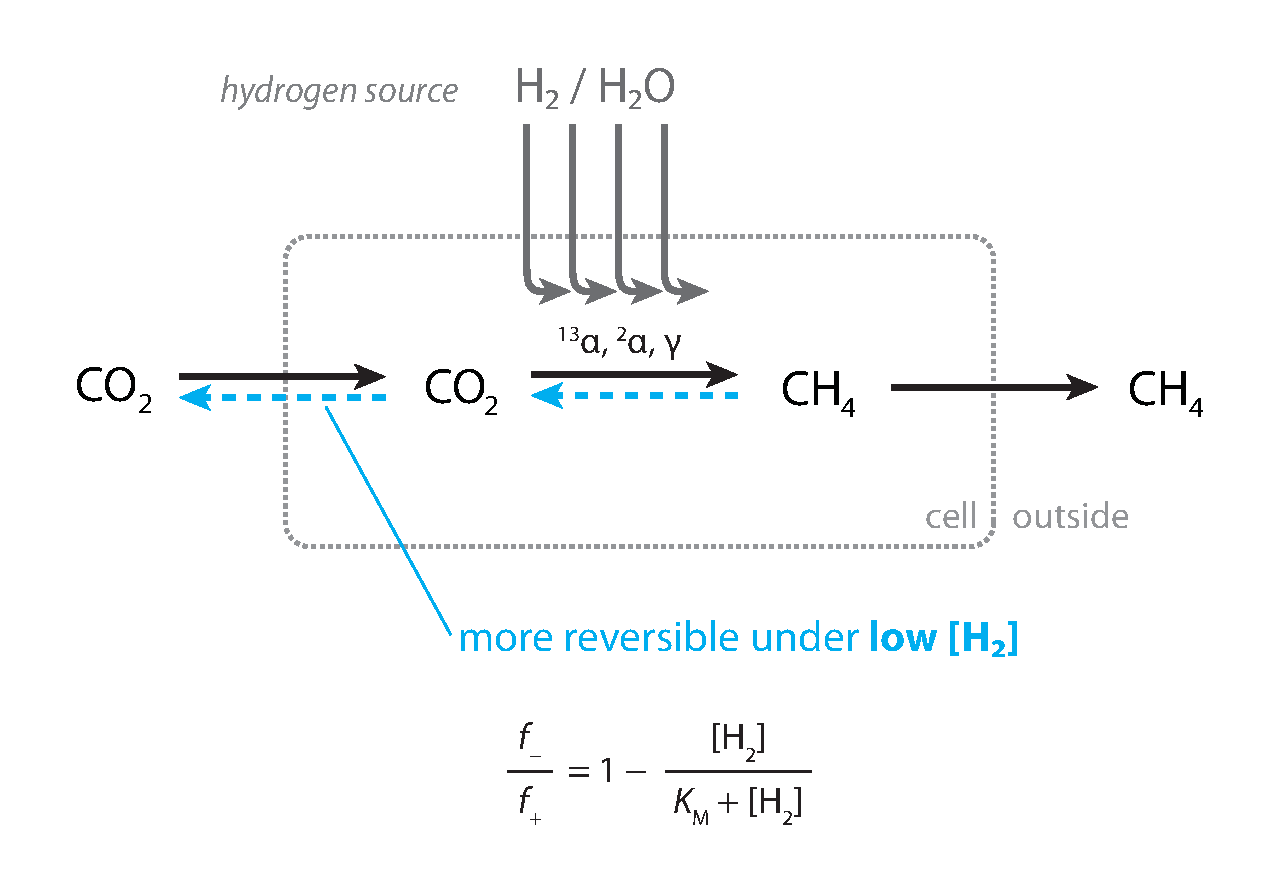
\includegraphics[width=0.6\textwidth]{figures/Fig1.6.pdf}
	\captionsetup{format=myformat}	% hrule beneath caption
	\caption[{Control of methane isotopologue abundances by reversibility and [H\textsubscript{2}] during methanogenesis}]{Preview of one of the main conclusions of \autoref{ch:2}:
		The isotopic composition of methane produced by methanogenesis is
		determined by reversibility, which in turn is related to free energy
		(for which the primary variable in most environments is H\textsubscript{2}
		concentration).}
	\label{fig:1:6}
\end{SCfigure*}

\begin{sidewaysfigure}
	\centering
	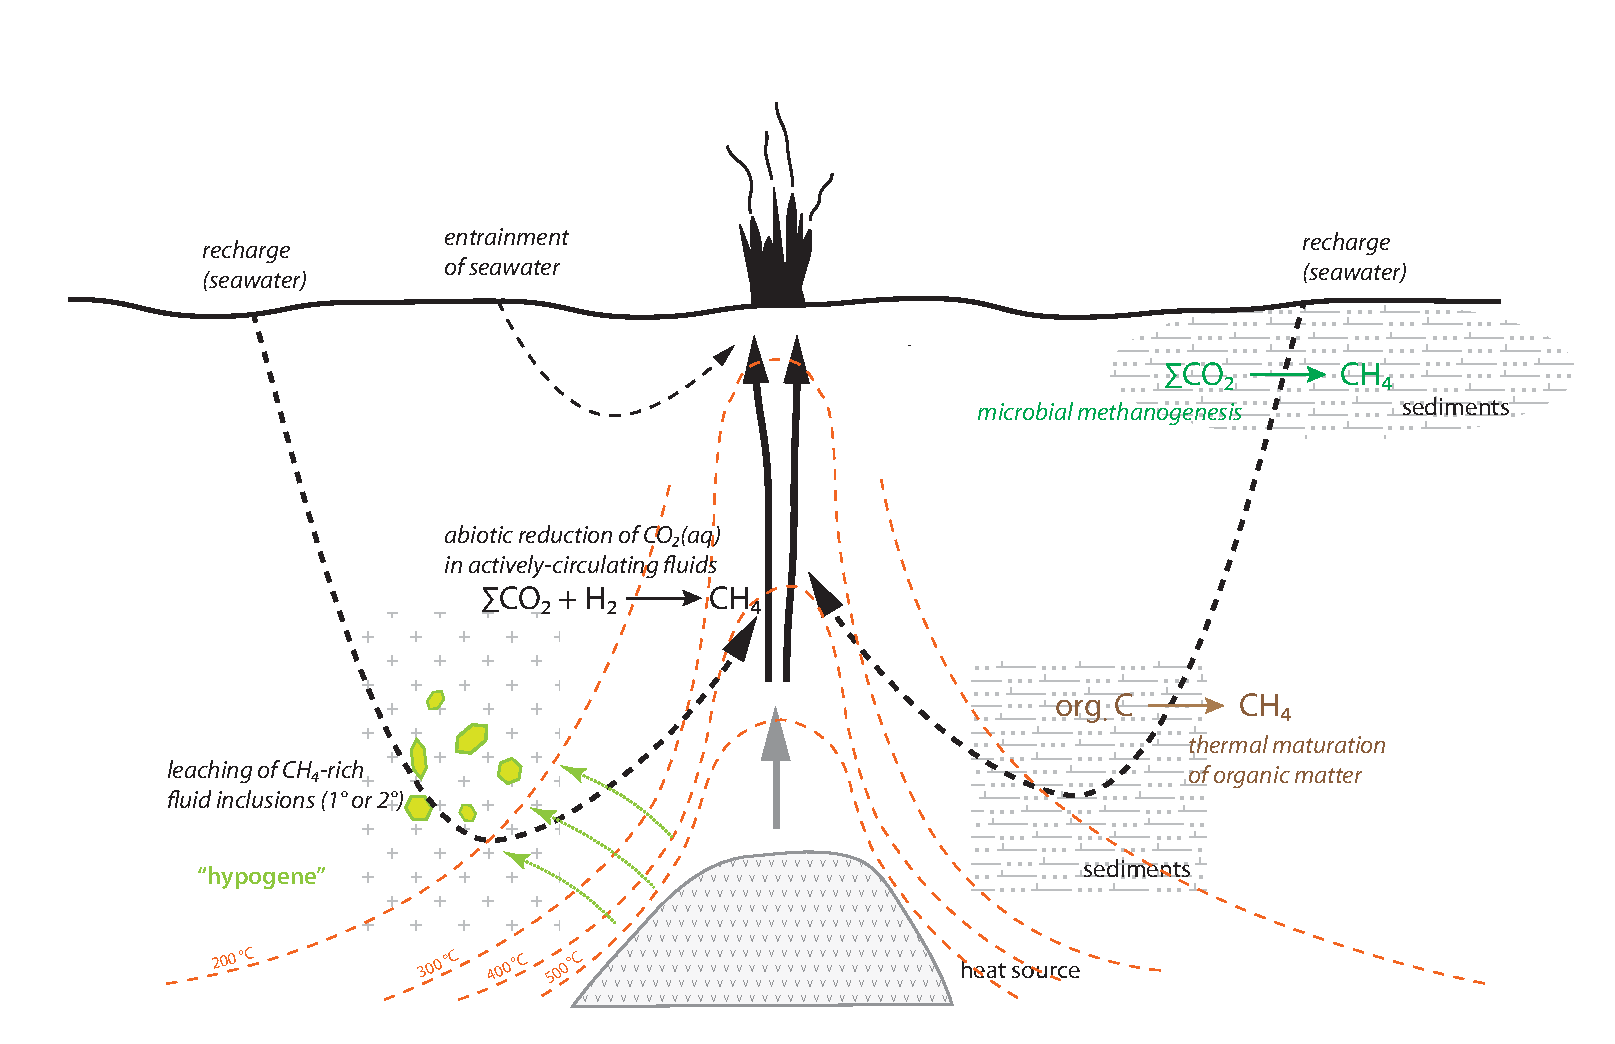
\includegraphics[width=0.95\textwidth]{figures/Fig1.7.pdf}
%	\captionsetup{format=myformat}	% hrule beneath caption
	\caption[Possible origins of methane at oceanic spreading centers]{Pathways for methane formation in mid-ocean ridge
		hydrothermal systems. \autoref{ch:3} shows how data from sediment-poor
		systems are most compatible with what we term a \emph{hypogene} origin
		for methane in vent fluids at oceanic spreading centers.}
	\label{fig:1:7}
\end{sidewaysfigure}

\autoref{ch:3} presents a study that attempts to address the oft-contentious
question of where and how methane in seafloor hydrothermal systems
forms. A diagram showing the several main proposed avenues for methane
formation in such systems is in \autoref{fig:1:7}. There is interest in knowing the
answer to this question because of potential implications for the origin
of life at deep-sea hot springs.

\autoref{ch:4} is an experimental and theoretical study that illustrates how
one major sink of methane in the environment, aerobic methanotrophy,
affects the isotopologue abundances of leftover methane (\autoref{fig:1:8}). The
results and equations can be generalized to other major methane sinks \parencite[including oxidation by OH and Cl in the atmosphere;][]{Whitehill++_2017_GCA}, and to other isotopologues (e.g.,
\textsuperscript{12}CH\textsubscript{2}D\textsubscript{2}).


\begin{SCfigure*}
	\centering
	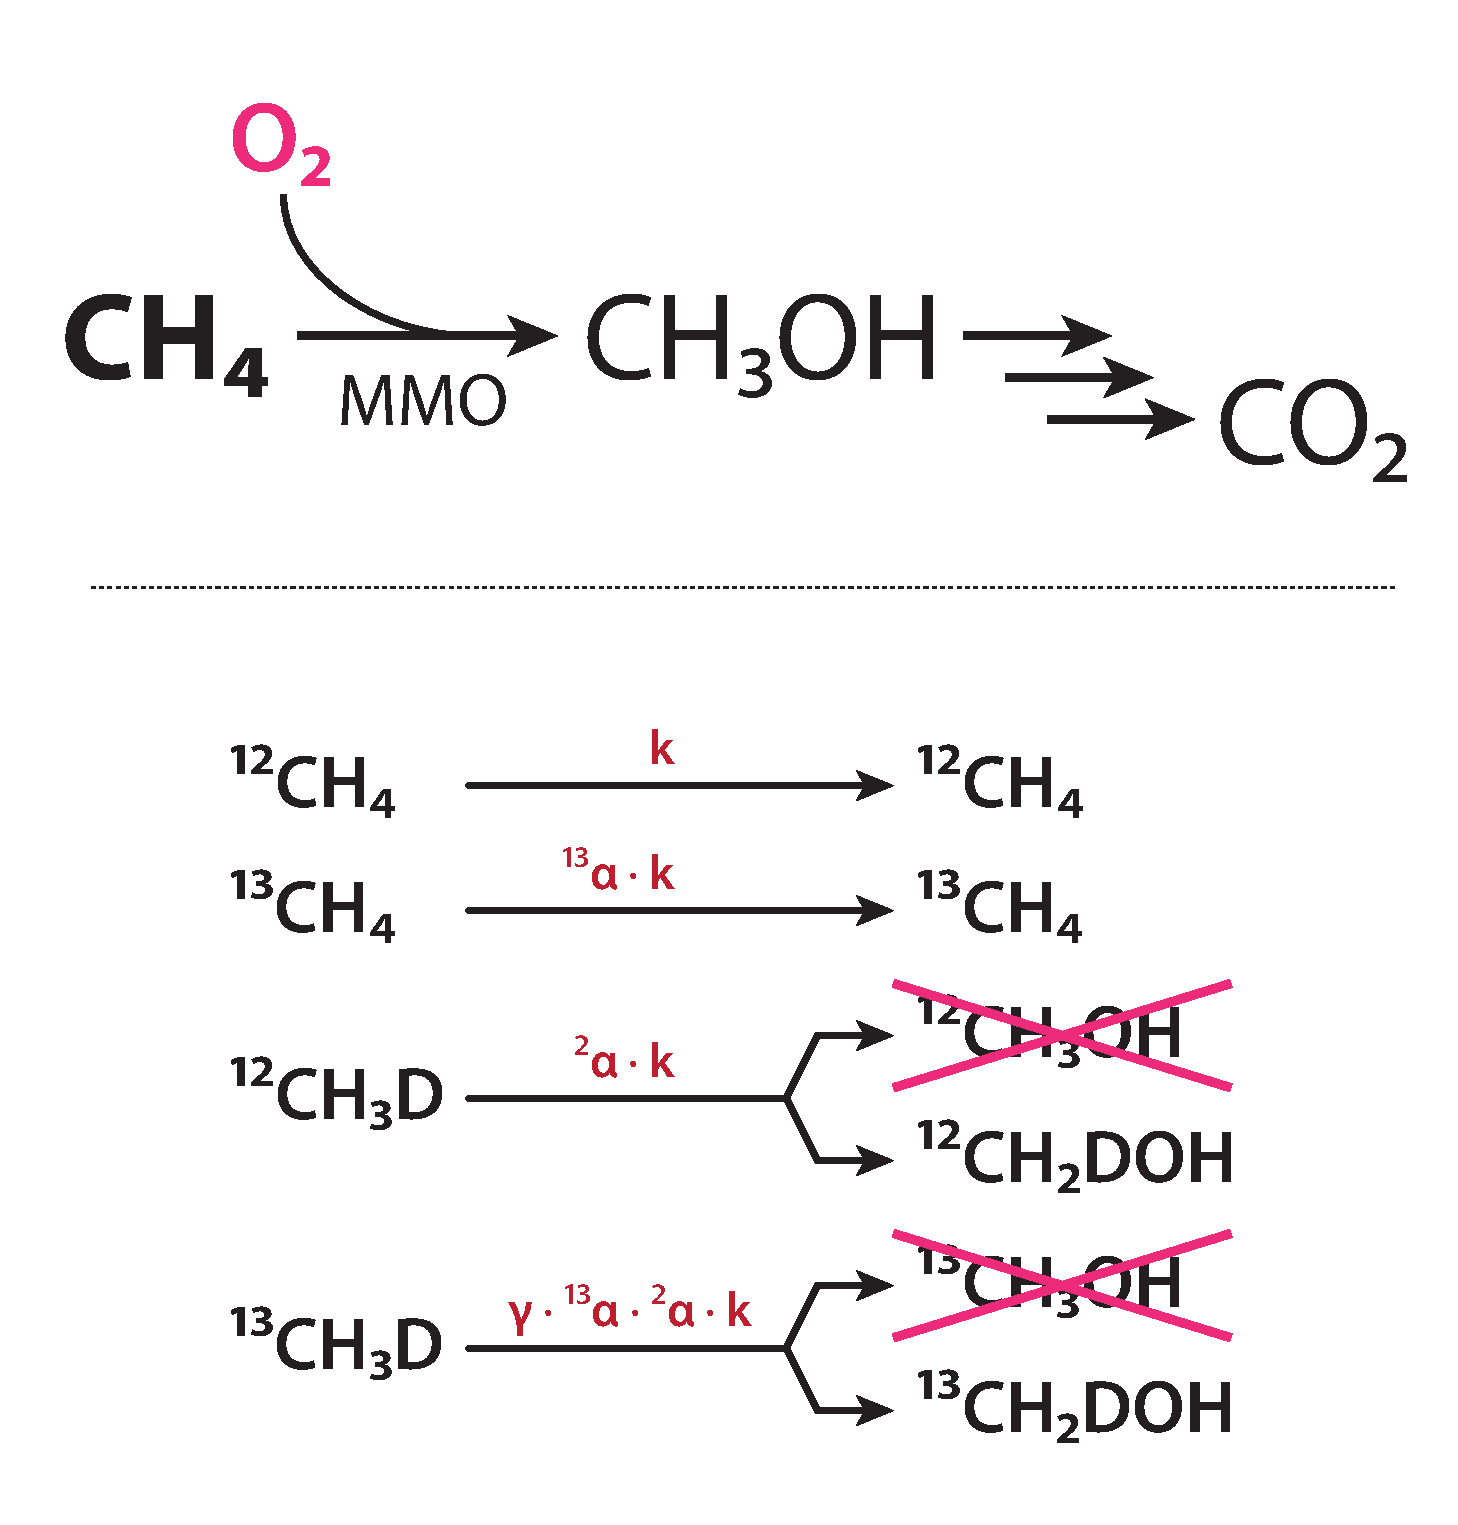
\includegraphics[width=0.45\textwidth]{figures/Fig1.8.pdf}
	\captionsetup{format=myformat}	% hrule beneath caption
	\caption[Reaction scheme for four stable isotopologues of methane during methane oxidation]{Reaction scheme for four stable isotopologues of
		methane during methane oxidation. Abstraction of D is
		\textasciitilde{}100× slower than H-abstraction. Substitution of D at an
		adjacent site has a small (\textasciitilde{}10\%)
		effect \parencite{Nesheim+Lipscomb_1996_Bc}. This means that
		the D/H fractionation comes mostly from the ¾ probability associated
		with abstraction of H from monodeuterated methane. 
		
		\quad \autoref{ch:4} and \textcite{Whitehill++_2017_GCA} show that
		fractionations are related by: 	\cee{\textsuperscript{13}CH\textsubscript{3}D/\textsuperscript{12}CH\textsubscript{4}
		= $\gamma$ × (\textsuperscript{13}C/\textsuperscript{12}C) × (D/H)},  where $\gamma$ is
		a number close to 1.000 (identical within error for OH and aerobic
		methanotrophy, and slightly less than 1 for Cl). Together, these
		fractionation factors constrain the effects on
		\textsuperscript{13}CH\textsubscript{3}D by the major methane sink
		reactions in the atmosphere and in oxic microbial habitats on Earth.}
	\label{fig:1:8}
\end{SCfigure*}

\begin{SCfigure*}
	\centering
	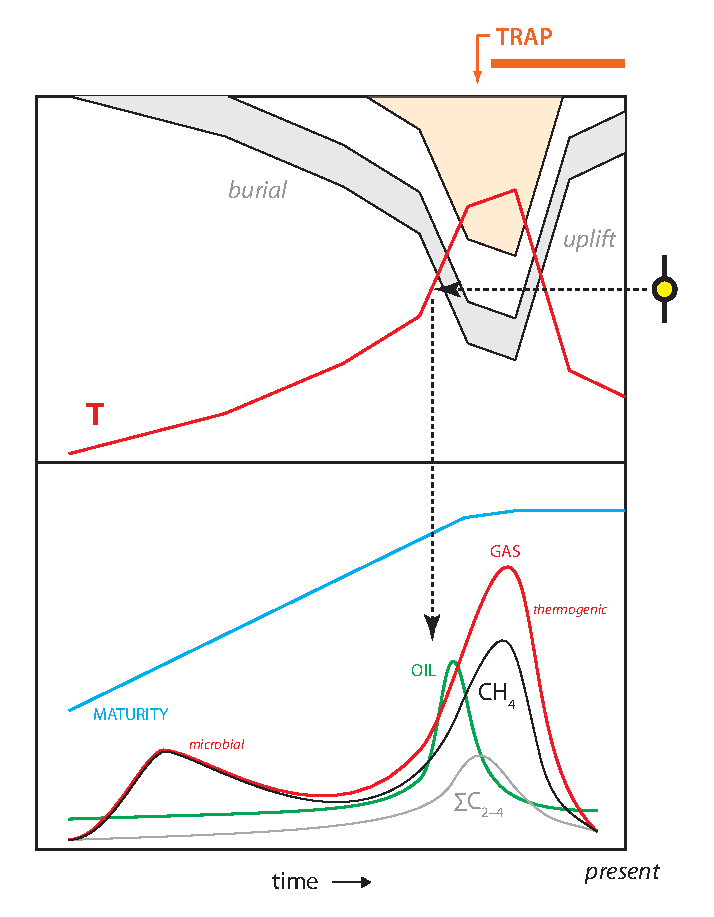
\includegraphics[width=0.6\textwidth]{figures/Fig1.9.pdf}
	\captionsetup{format=myformat}	% hrule beneath caption
	\caption[Petroleum system applications of
	\textsuperscript{13}CH\textsubscript{3}D]{Petroleum system applications of
		\textsuperscript{13}CH\textsubscript{3}D. The potential application
		space of methane isotopologue geothermometry and geospeedometry include
		the ability to link key hydrocarbon system elements (particularly
		elements of source, charge, and trap) in time and space, to calibrate
		and/or validate basin model predictions and coupled source rock
		maturation simulations, and to define a new metric of maturity based
		solely on fluid chemistry.}
	\label{fig:1:9}
\end{SCfigure*}

Research on the behavior of methane isotopologues like
\textsuperscript{13}CH\textsubscript{3}D have a natural alignment to
many of the questions that are important and possibly unanswered in
assessment of petroleum systems, particularly in poorly understood
basins (\autoref{fig:1:9}). In particular, measurements of methane isotopologues can
\begin{itemize}
	\item
	place quantitative constraints on the stability and origin of C--H
	bonds in hydrocarbons in the Earth's subsurface;
	\item
	test interpretive models of natural gas composition and gas isotope
	systematics; and
	\item
	be used to help anchor the chemistry of natural gases to time and
	temperature.
\end{itemize}

\mrefs[]{Appendices}{dx:A} and \ref{dx:B} represent some initial efforts to read the
hydrogen-isotope and clumped isotopologue record of natural gases and
define what those records mean.

\autoref{dx:C} offers miscellaneous tricks, tips, and data that didn't fit
anywhere else.


























	\chapter{Nonequilibrium clumped isotope signals in microbial methane}
\label{ch:2}
\chaptermark{Survey of \ce{^{13}CH3D in the environment}}




\begin{abstract}
	\noindent Methane is a key component in the global carbon cycle with a wide range
	of anthropogenic and natural sources. While isotopic compositions of
	methane have traditionally aided source identification, the abundance of
	its multiply-substituted ``clumped'' isotopologues (e.g.,
	\textsuperscript{13}CH\textsubscript{3}D) has recently emerged as
	a proxy for determining methane-formation temperatures. However, the
	impact of biological processes on methane's clumped isotopologue
	signature is poorly constrained. Here, we show that methanogenesis
	proceeding at relatively high rates in cattle, surface environments, and
	laboratory cultures exerts kinetic control on
	\textsuperscript{13}CH\textsubscript{3}D abundances and results in
	anomalously elevated formation temperature estimates. We demonstrate
	quantitatively that H\textsubscript{2} availability accounts for this
	effect. Clumped methane thermometry can therefore provide
	constraints on the generation of methane in diverse settings, including
	continental serpentinization sites and ancient, deep groundwaters.
\end{abstract}

\vspace*{\fill}

\noindent \rule{\textwidth}{0.4pt}\\

{\small
	
	\noindent A version of this chapter has been published as:\\
	
	\noindent Wang, D. T.; Gruen, D. S.; Lollar, B. S.; Hinrichs, K.-U.; Stewart, L. C.; Holden, J. F.; Hristov, A. N.; Pohlman, J. W.; Morrill, P. L.; Könneke, M.; Delwiche, K. B.; Reeves, E. P.; Sutcliffe, C. N.; Ritter, D. J.; Seewald, J. S.; McIntosh, J. C.; Hemond, H. F.; Kubo, M. D.; Cardace, D.; Hoehler, T. M. \& Ono, S. (2015) Nonequilibrium clumped isotope signals in microbial methane. \emph{Science,} \textbf{348}, 428--431.  \href{http://dx.doi.org/10.1126/science.aaa4326}{\nolinkurl{doi: 10.1126/science.aaa4326}}\\
	
	\noindent Copyright © 2015, The Authors.  AAAS maintains exclusive rights to use and authorize use of this article under its License to Publish.  Reproduction in this thesis is permitted under the terms of this agreement.
	
}

\clearpage

\section{Main Text} \label{main-text}
%\addcontentsline{toc}{section}{\protect\numberline{}Main Text}
%\addcontentsline{toc}{section}{Main Text}


\noindent Carbon (\textsuperscript{13}C/\textsuperscript{12}C) and hydrogen (D/H)
isotope ratios of methane are widely applied for distinguishing
microbial from thermogenic methane in the environment \parencite{Baldassare++_2014_AAPGB,Flores++_2008_IJCG,Pohlman++_2009_EPSL,SherwoodLollar++_2008_GCA,SherwoodLollar++_2002_N,Welhan+Lupton_1987_AAPGB,Whiticar_1990_OG} as well as for apportioning pathways of microbial
methane production \parencite{Burke++_1988_N,McCalley++_2014_N,Whiticar++_1986_GCA}. This bulk isotope approach,
however, is largely based on empirical observations, and different
origins of methane often yield overlapping characteristic isotope
signals \parencite{Pohlman++_2009_EPSL,Whiticar_1990_OG,Etiope+SherwoodLollar_2013_RG,Schoell_1988_CG,Whiticar_1999_CG}. Beyond conventional
bulk isotope ratios, it has become possible to precisely measure the
abundance of multiply-substituted ``clumped'' isotopologues (e.g.,
\textsuperscript{13}CH\textsubscript{3}D) \parencite{Ono++_2014_AC,Stolper++_2014_GCA}. In
particular, the abundances of clumped isotopes makes it possible to obtain information
about the temperature at which C--H bonds were formed or last
equilibrated \parencite[][and \autoref{fig:2:S1}]{Ono++_2014_AC}. Formation temperatures
of both thermogenic and microbial methane in natural gas reservoirs can
be estimated on the basis of clumped isotopologues \parencite{Stolper++_2014_S}. The
mechanisms by which isotopologues attain distributions consistent with
thermodynamic equilibrium, however, remain unclear because bulk methane
isotopes (δ\textsuperscript{13}C and δD) often reflect kinetic isotope
fractionations \parencite{Whiticar_1999_CG,Valentine++_2004_GCA}, and H-isotope exchange between
methane and water is sluggish \parencite{Reeves++_2012_GCA}.

To test if clumped methane thermometry can be widely applied for methane
sources beyond natural gas reservoirs, we examined methane samples from
diverse systems, including lakes, wetlands, cow rumen, laboratory
cultures of methanogenic microbes, and geological settings that may
support abiogenic methane production. We measured the relative abundances of four methane
isotopologues (\textsuperscript{12}CH\textsubscript{4},
\textsuperscript{13}CH\textsubscript{4},
\textsuperscript{12}CH\textsubscript{3}D and
\textsuperscript{13}CH\textsubscript{3}D) using a recently-developed
tunable laser spectroscopy technique \parencite[][and \autoref{materials-and-methods}]{Ono++_2014_AC}.


\begin{SCfigure*}[][htbp]
	\centering
	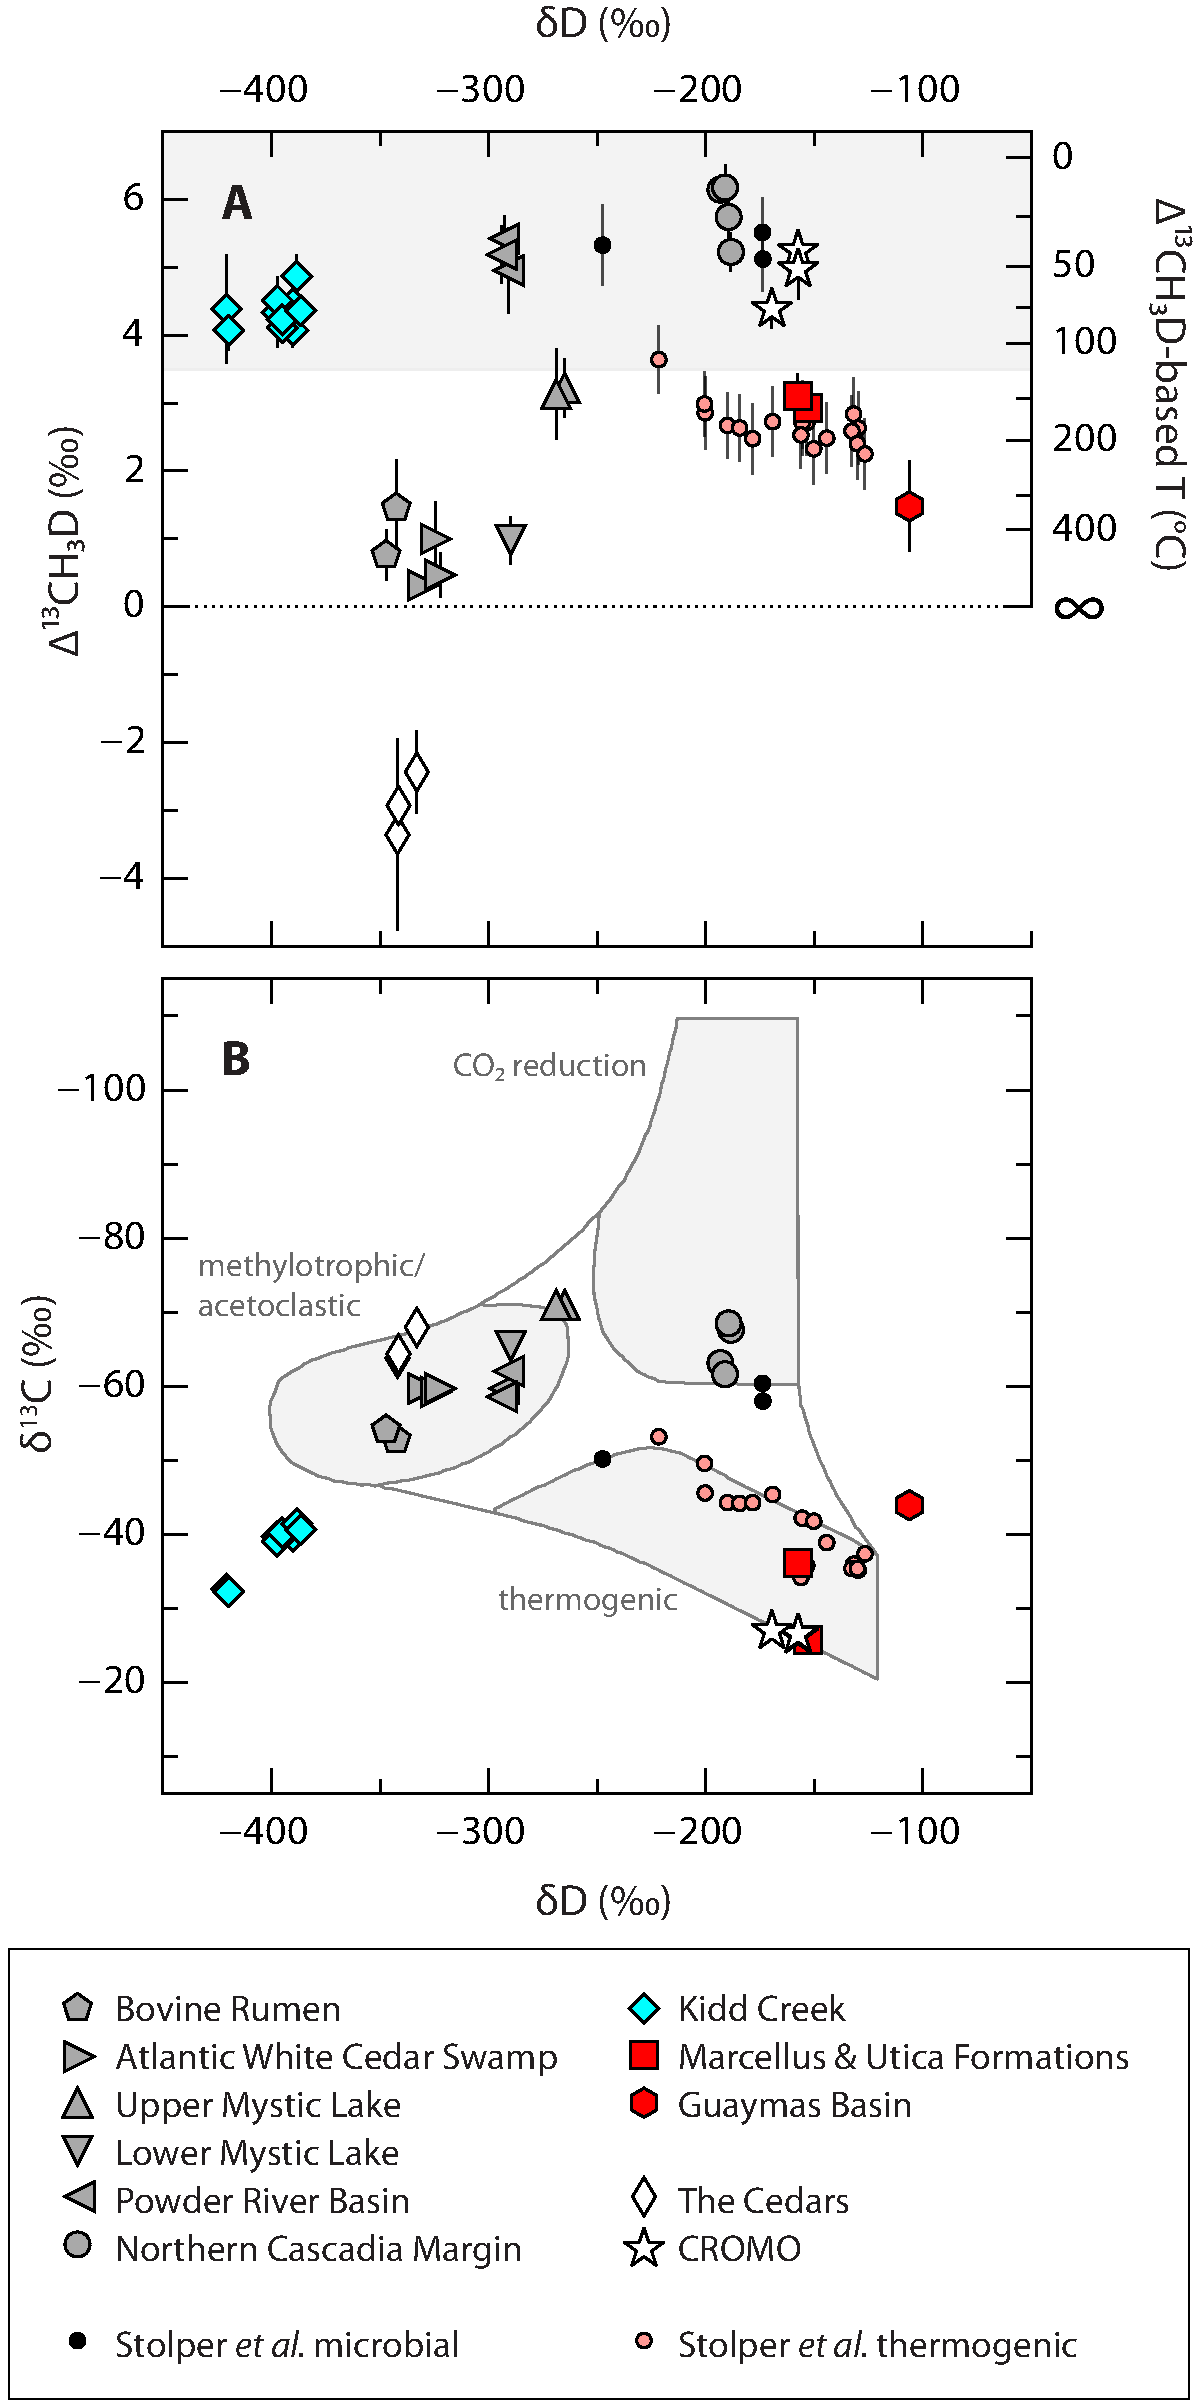
\includegraphics[width=0.5\linewidth]{figures/Fig2.1}
	\caption[Isotopologue compositions of methane samples from an environmental survey]{Isotopologue compositions of methane samples. \textbf{(A)}
	Δ\textsuperscript{13}CH\textsubscript{3}D plotted against δD. The
	Δ\textsuperscript{13}CH\textsubscript{3}D temperature scale corresponds
	to calibration in \autoref{fig:2:S1}. Error bars are 95\% confidence intervals
	(\autoref{tab:2:S1}). Data from \textcite{Stolper++_2014_S} were scaled to their
	corresponding Δ\textsuperscript{13}CH\textsubscript{3}D values
	\parencite{Stolper++_2014_GCA}. The shaded area represents the temperature range within
	which microbial life has been demonstrated to date \parencite{Takai++_2008_PNAS}. The
	hatched line represents Δ\textsuperscript{13}CH\textsubscript{3}D = 0‰ (\textit{T} → $\infty$); data plotting below this line cannot yield corresponding
	apparent temperatures. \textbf{(B)} δ\textsuperscript{13}C plotted
	against δD, showing characteristic fields for different methane sources
	from \textcite{Whiticar_1999_CG}.}
	\label{fig:2:1}
\end{SCfigure*}


Our measurements for dominantly-thermogenic gases from the Marcellus and
Utica Shales \parencite{Baldassare++_2014_AAPGB,Burruss+Laughrey_2010_OG} yielded
Δ\textsuperscript{13}CH\textsubscript{3}D-based temperatures of $147^{+25}_{-22}$\,°C and $160^{+29}_{-25}$\,°C, respectively. The clumped-isotope temperature for the Marcellus
Shale sample is comparable to, although slightly lower than, estimates
by \textcite{Stolper++_2014_S} of 179--207~°C (\autoref{fig:2:1}). In addition,
microbial methane in pore waters and gas hydrates from northern Cascadia
margin sediments \parencite{Pohlman++_2009_EPSL}, and from wells producing from coal seams in
the Powder River Basin \parencite{Flores++_2008_IJCG,Bates++_2011_CG} yielded
Δ\textsuperscript{13}CH\textsubscript{3}D temperatures of 12--42~°C and
35--52~°C, respectively. These are consistent with their expected low
formation temperatures. Furthermore, thermogenic methane sampled from a
hydrothermal vent in the Guaymas Basin, Gulf of California \parencite{Welhan+Lupton_1987_AAPGB},
yielded a Δ\textsuperscript{13}CH\textsubscript{3}D temperature of $326^{+170}_{-95}$\,°C,
within error of the measured vent temperature \parencite[299~°C;][]{Reeves++_2014_PNAS}.
Therefore, our data provide independent support of the hypothesis that
\textsuperscript{13}CH\textsubscript{3}D abundance reflects the
temperature at which methane is generated in these sedimentary basins
\parencite{Stolper++_2014_S}.

In contrast, we found that methane sampled from lakes, a swamp, and the
rumen of a cow carry \textsuperscript{13}CH\textsubscript{3}D signals
that correspond to anomalously high
Δ\textsuperscript{13}CH\textsubscript{3}D temperatures (139--775~°C,
\mrefs[A]{Fig.}{fig:2:1}) that are well above the environmental temperatures (\textless{}40~°C). Such signals are clearly not controlled by equilibrium. Notably, a
positive correlation between Δ\textsuperscript{13}CH\textsubscript{3}D
and the extent of D/H fractionation between methane and environmental
water [$\varepsilon$\textsubscript{methane/water};\footnote{\label{fn:2:epsilon}The abundance of \textsuperscript{13}CH\textsubscript{3}D is
	captured by a metric, Δ\textsuperscript{13}CH\textsubscript{3}D, which
	quantifies its deviation from a random distribution of isotopic
	substitutions amongst all isotopologues in a sample of methane:
	Δ\textsuperscript{13}CH\textsubscript{3}D = ln\,\emph{Q}, where \emph{Q}
	is the reaction quotient of the isotope exchange reaction:
	$ {}^{13}\text{CH}_4+ {}^{12}{\text{CH}}_3\text{D}\rightleftharpoons {}^{13}{\text{CH}}_3\text{D}+ {}^{12}{\text{CH}}_4 $, where the δ-values are
	conventional isotopic notation, e.g., δD =
	(D/H)\textsubscript{sample}/(D/H)\textsubscript{reference} $-$ 1. Mass
	spectrometric measurements yield Δ\textsubscript{18}, a parameter that
	quantifies the combined abundance of
	\textsuperscript{13}CH\textsubscript{3}D and
	\textsuperscript{12}CH\textsubscript{2}D\textsubscript{2}. For most
	natural samples of methane, Δ\textsubscript{18} is expected to be
	directly-relatable to Δ\textsuperscript{13}CH\textsubscript{3}D as
	measured by laser spectroscopy. The D/H fractionation between methane
	and environmental water is defined as $\varepsilon$\textsubscript{methane/water} =
	(D/H)\textsubscript{methane}/(D/H)\textsubscript{water} $-$ 1.} \autoref{fig:2:2}] suggests
a strong link between isotopologue (i.e.,
\textsuperscript{13}CH\textsubscript{3}D) and isotope (D/H)
disequilibria. In contrast, the above mentioned methane samples from
sedimentary basins appear to have attained hydrogen-isotope equilibrium
with associated waters at or near the temperatures indicated by the
Δ\textsuperscript{13}CH\textsubscript{3}D data (\autoref{fig:2:2}).

To confirm these observations from the natural environment, we
demonstrated that strong disequilibrium
\textsuperscript{13}CH\textsubscript{3}D signals are also produced by
cultures of methanogenic archaea in the laboratory (\autoref{fig:2:3}).
Thermophilic methanogens cultured at 40 to 85~°C produced methane with
Δ\textsuperscript{13}CH\textsubscript{3}D values from +0.5 to +2.3‰
(corresponding to Δ\textsuperscript{13}CH\textsubscript{3}D temperatures
of 216--620~°C), and mesophilic methanogens cultured at ambient
temperature produced methane with conspicuously ``anti-clumped''
signatures (i.e., values of Δ\textsuperscript{13}CH\textsubscript{3}D
\textless{} 0‰, for which no apparent temperature can be expressed) as
low as $-$1.3‰ (\autoref{fig:2:3}). Methane from cultures is also characterized by
large kinetic D/H fractionation with respect to water \parencite{Valentine++_2004_GCA,Balabane++_1987_OG}. Because laboratory cultures are grown under optimal
conditions (high H\textsubscript{2} and high CO\textsubscript{2}), these
anti-clumped Δ\textsuperscript{13}CH\textsubscript{3}D and low
$\varepsilon$\textsubscript{methane/water} values are primarily expressions of
kinetic isotope effects. Consequently, the distribution of samples with
Δ\textsuperscript{13}CH\textsubscript{3}D and
$\varepsilon$\textsubscript{methane/water} values in \autoref{fig:2:2} can be explained by
microbial methanogenesis operating on a spectrum between fully kinetic
(low Δ\textsuperscript{13}CH\textsubscript{3}D and low
$\varepsilon$\textsubscript{methane/water}) and equilibrium (high
Δ\textsuperscript{13}CH\textsubscript{3}D and high
$\varepsilon$\textsubscript{methane/water}) end-members.

We constructed a mathematical framework to describe the controls on the
correlation of Δ\textsuperscript{13}CH\textsubscript{3}D and
$\varepsilon$\textsubscript{methane/water} signals from hydrogenotrophic
methanogenesis. The model largely follows those developed for microbial
sulfate reduction \parencite{Rees_1973_GCA,Wing+Halevy_2014_PNAS} and predicts the isotopologue
compositions of product methane as a result of a series of enzymatic
reactions (\autoref{fig:2:S4} and \autoref{model-of-isotopologue-systematics-during-microbial-methanogenesis}). Using isotope fractionation
factors estimated from theory, experiments, and observations as input
parameters (\autoref{tab:2:S3}), our model reproduces the
observed correlation between Δ\textsuperscript{13}CH\textsubscript{3}D
and $\varepsilon$\textsubscript{methane/water} of natural samples (\autoref{fig:2:2}). The
isotopologue compositions of product methane reflect the degree of
metabolic reversibility. Fully reversible reactions yield equilibrium
end-members \parencite{Holler++_2011_PNAS}, while irreversible reactions result in kinetic
(disequilibrium) end-member signals. In this model, the reversibility is
linked to available free energy \parencite{Holler++_2011_PNAS,Wing+Halevy_2014_PNAS}, in this case
expressed as H\textsubscript{2} concentration
({[}H\textsubscript{2}{]}). The model can explain the relationship among
{[}H\textsubscript{2}{]}, $\varepsilon$\textsubscript{methane/water} \parencite{Burke_1993_Chemosphere}, and
Δ\textsuperscript{13}CH\textsubscript{3}D via Michaelis-Menten kinetics,
and can predict the patterns observed in diverse settings ranging from
marine sediments (low {[}H\textsubscript{2}{]}, high
Δ\textsuperscript{13}CH\textsubscript{3}D and
$\varepsilon$\textsubscript{methane/water}) to bovine rumen (high
{[}H\textsubscript{2}{]}, low Δ\textsuperscript{13}CH\textsubscript{3}D
and $\varepsilon$\textsubscript{methane/water}) (\autoref{fig:2:4}). We note that mixing of
methane sources with different δ\textsuperscript{13}C and δD values or
oxidation of methane could also alter the relationships over the primary
signal of microbial methanogenesis (\autoref{evaluation-of-alternative-mechanisms-for-isotopic-disequilibria-in-microbial-methane}). Likewise, inheritance of
clumping signals from precursor organic substrates (e.g., via
acetoclastic or methylotrophic methanogenesis) cannot be entirely ruled
out and awaits experimental validation.

We showed above that the combination of
Δ\textsuperscript{13}CH\textsubscript{3}D and
$\varepsilon$\textsubscript{methane/water} values provides mechanistic constraints
on whether methane was formed under kinetic vs.\ near-equilibrium
conditions. Next, we used this framework to place constraints on the
origins of methane at two sites of present-day serpentinization in
Phanerozoic ophiolites {[}The Cedars \parencite{Morrill++_2013_GCA} and Coast Range
Ophiolite Microbial Observatory, CROMO \parencite{Cardace++_2013_SD}{]} in northern
California, and in deep (\textgreater{} 2 km below surface) fracture
fluids with billion year-residence times in the Kidd Creek mine, Canada
\parencite{SherwoodLollar++_2002_N,Holland++_2013_N}.

Methane collected from groundwater springs associated with
serpentinization at The Cedars yielded anti-clumped
Δ\textsuperscript{13}CH\textsubscript{3}D signals ($-$3‰) with low
$\varepsilon$\textsubscript{methane/water} values (\mrefs[A]{Figs.}{fig:2:1} and \ref{fig:2:2}). The data plot
along the microbial (kinetic) trend defined in \autoref{fig:2:2}, supporting a
previous hypothesis that methane at The Cedars is being produced by
active microbial methanogenesis \parencite{Morrill++_2013_GCA}. The exceptionally high
H\textsubscript{2} concentration (up to 50\% by volume in bubbles) at The Cedars indicates the
massive excess of electron donor. This, along with severe inorganic
carbon limitation {[}due to high pH (\textgreater{}11) and precipitation
of carbonate minerals \parencite{Morrill++_2013_GCA}{]}, drives the formation of methane
carrying strong kinetic imprints, consistent with the observed
anti-clumped Δ\textsuperscript{13}CH\textsubscript{3}D signals (\autoref{fig:2:4}).




\begin{SCfigure*}[][p]
	\centering
	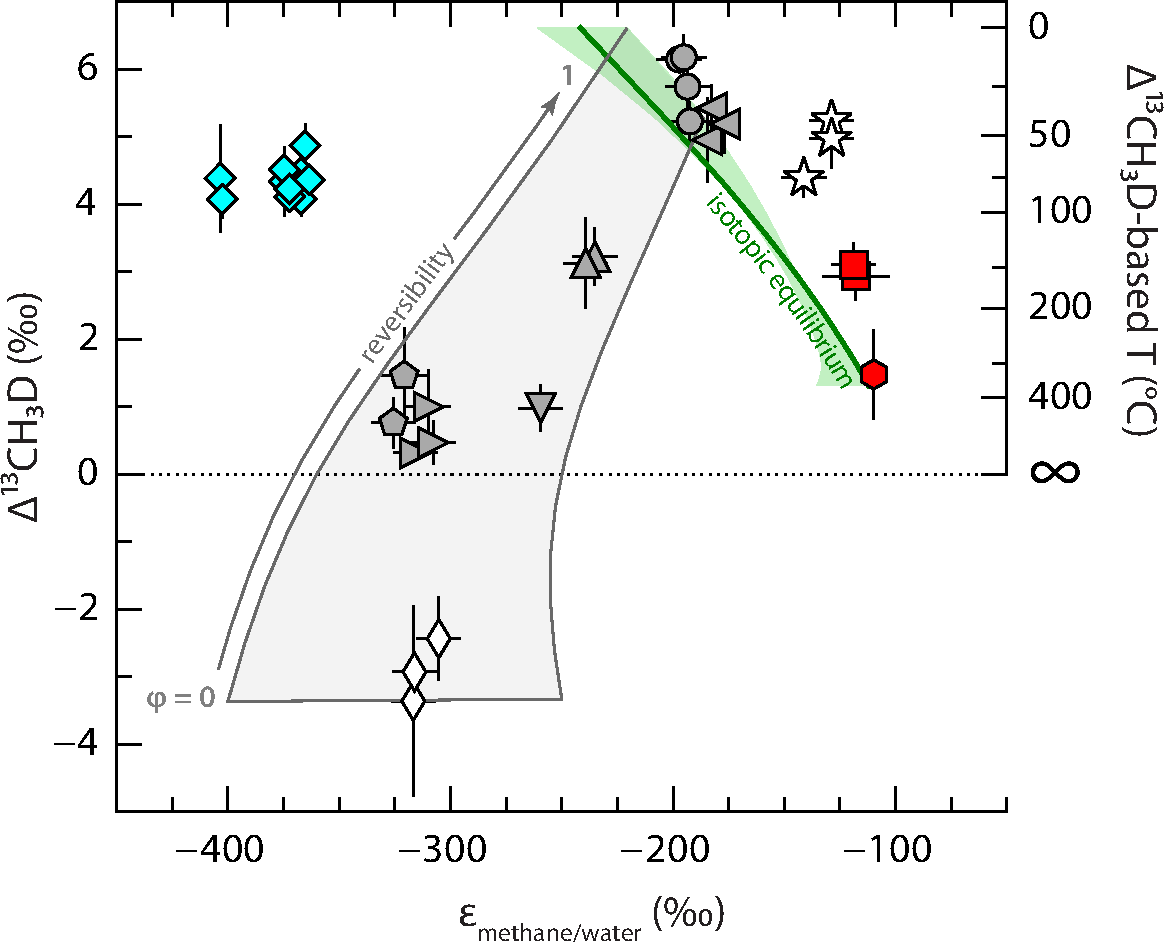
\includegraphics[width=0.5\linewidth]{figures/Fig2.2}
	\caption[Extent of clumped- and hydrogen-isotopic disequilibria in methane]{Extent of clumped- and hydrogen-isotopic disequilibria in methane. Symbols and vertical error bars are the same as those in \autoref{fig:2:1}.
	Horizontal error bars represent uncertainties on estimates of
	$\varepsilon$\textsubscript{methane/water}\footref{fn:2:epsilon} (\autoref{tab:2:S4}). The solid
	green curve represents isotopic equilibrium, with the
	$\varepsilon$\textsubscript{methane/water} calibration given by \textcite{Horibe+Craig_1995_GCA}. Green
	shading represents ranges of $\varepsilon$\textsubscript{methane/water} calibrations
	from published reports (\autoref{fig:2:S3}). Gray shading represents model
	predictions from this study for microbial methane formed between 0 and
	40~°C. Metabolic reversibility ($\varphi$) increases from bottom ($\varphi$ = 0,
	fully-kinetic) to top ($\varphi$ → 1, equilibrium) within this field
	(see \autoref{model-of-isotopologue-systematics-during-microbial-methanogenesis}).}
	\label{fig:2:2}
\end{SCfigure*}

\begin{SCfigure*}[][p]
	\centering
	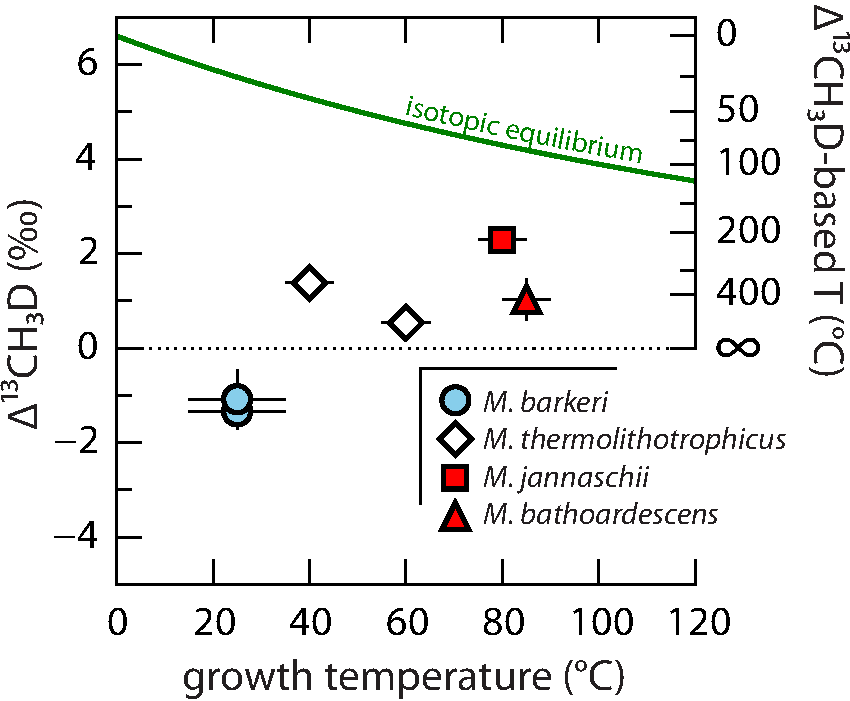
\includegraphics[width=0.37\linewidth]{figures/Fig2.3}
	\caption[Δ\textsuperscript{13}CH\textsubscript{3}D values of methane produced
	by hydrogenotrophic methanogens in batch cultures]{Δ\textsuperscript{13}CH\textsubscript{3}D values of me\-thane produced
		by hydro\-geno\-trophic methan\-ogens in batch cultures reflect kinetic
		effects. Data and error bars are from \autoref{tab:2:S2}. The green line
	represents clumped isotopologue equilibrium (i.e., samples for which
	Δ\textsuperscript{13}CH\textsubscript{3}D temperature is equal to growth
	temperature; \autoref{fig:2:S1}).}
	\label{fig:2:3}
\end{SCfigure*}
\begin{SCfigure*}[][p]
	\centering
	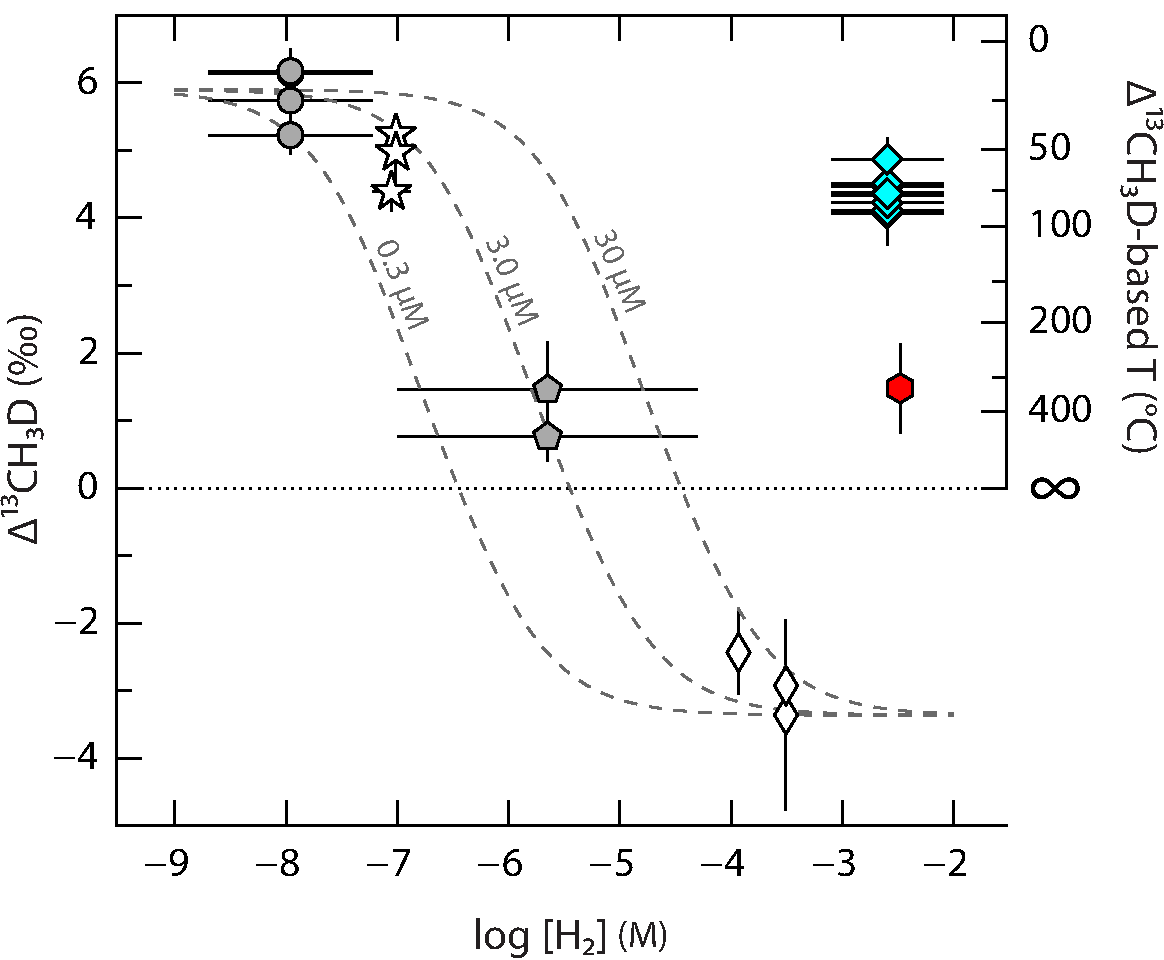
\includegraphics[width=0.5\linewidth]{figures/Fig2.4}
	\caption[Relationships between
	Δ\textsuperscript{13}CH\textsubscript{3}D and H\textsubscript{2}
	concentration for microbial methane]{Relationships between
		Δ\textsuperscript{13}CH\textsubscript{3}D and H\textsubscript{2}
		concentration for microbial methane. Symbols and vertical error bars
	are the same as in \autoref{fig:2:1}. The H\textsubscript{2} data are from \autoref{tab:2:S4}; when a range of {[}H\textsubscript{2}{]} values is given, points are
	plotted at the geometric mean of the maximum and minimum values. Dashed
	lines represent model predictions for microbial methane produced at 20~°C, calculated using \emph{K}\textsubscript{M}'s of 0.3, 3.0, and 30~µM
	H\textsubscript{2}. Data for samples of dominantly non-microbial methane
	from Guaymas Basin and Kidd Creek are plotted for comparison.}
	\label{fig:2:4}
\end{SCfigure*}


Despite the similarity in geologic setting, methane associated with
serpentinization at CROMO \parencite{Cardace++_2013_SD} revealed very different
Δ\textsuperscript{13}CH\textsubscript{3}D values that correspond to
low apparent temperatures (42--76~°C) and plot close to the equilibrium
line (\autoref{fig:2:2}). While the conventional δ\textsuperscript{13}C and δD
values of methane from CROMO are nearly identical to those of the Utica
Shale sample (\mrefs[B]{Fig.}{fig:2:1}), methane at CROMO carries much higher
Δ\textsuperscript{13}CH\textsubscript{3}D values (\mrefs[A]{Fig.}{fig:2:1}). The origin
of methane at the CROMO site remains unresolved \parencite{Cardace++_2013_SD}, but the
comparably high Δ\textsuperscript{13}CH\textsubscript{3}D values at
CROMO suggest that methane here could be sourced from a mixture of
thermogenic and microbial methane. Alternatively, lower
H\textsubscript{2} availability at CROMO compared to The Cedars (\autoref{tab:2:S4}), may support microbial methanogenesis under near-equilibrium
conditions (\autoref{fig:2:4}). Regardless, the different isotopologue signatures
in methane from CROMO vs.\ The Cedars demonstrate that distinct processes
contribute to methane formation in these two serpentinization systems.

Deep, ancient fracture fluids in the Kidd Creek mine in the Canadian
Shield \parencite{Holland++_2013_N} contain copious quantities of both dissolved methane
and hydrogen \parencite{SherwoodLollar++_2002_N}. The Kidd Creek methane occupies a distinct
region in the Δ\textsuperscript{13}CH\textsubscript{3}D vs.\ $\varepsilon$\textsubscript{methane/water} diagram (\autoref{fig:2:2}), due to strong D/H
disequilibria between methane and water \parencite{SherwoodLollar++_2008_GCA} and low
Δ\textsuperscript{13}CH\textsubscript{3}D temperature signals of 56--90~°C that are consistent with other temperature estimates for these
groundwaters \parencite{SherwoodLollar++_2008_GCA}. Although the specific mechanisms by which the
proposed abiotic hydrocarbons at Kidd Creek are generated remain under
investigation \parencite{SherwoodLollar++_2002_N,SherwoodLollar++_2014_N}, the distinct isotopologue signals
provide further support for the hypothesis that methane here is neither
microbial nor thermogenic.

Our results demonstrate that measurements of
\textsuperscript{13}CH\textsubscript{3}D provide information beyond the
simple formation temperature of methane. The combination of methane/water
D/H fractionation and
\textsuperscript{13}CH\textsubscript{3}D abundance enables the
differentiation of methane that has been formed at extremely low rates
in the subsurface \parencite{Pohlman++_2009_EPSL,Bates++_2011_CG,Holler++_2011_PNAS} from methane formed
in cattle and surface environments in which methanogenesis proceeds at
comparatively high rates \parencite{Johnson+Johnson_1995_JAnimalSci,Varadharajan+Hemond_2012_JGR}.
\blfootnote{\textsc{note added during thesis preparation}: I do not favor the use of the term \emph{formation temperature}. 
This term has a distinct and widely-accepted meaning in industries associated with subsurface resources (particularly within the disciplines
of formation evaluation, reservoir engineering, and petrophysics).  Practitioners of isotope geochemistry can better communicate by using 
less-ambiguous wording such as \emph{temperatures of methane generation} and \emph{clumped isotopologue temperatures}. 
The distinction between these two concepts is important because---as this thesis demonstrates---apparent temperatures 
derived from equilibria between methane isotopologues are often different from the temperatures at which methane 
was generated.  Methane may also be generated at one temperature, and later ``scrambled'' (its C--H bonds 
rearranged/equilibrated) at a different temperature; only the temperature of last equilibration would be 
recorded by Δ\textsuperscript{13}CH\textsubscript{3}D values.} 
 %This approach provides
%a new window for interrogating the biochemistry of methanogenesis in
%nature.

\clearpage



\section{Acknowledgments}\label{acknowledgments}
%\textbf{Acknowledgments.} 
%\addcontentsline{toc}{section}{Acknowledgments}
We thank J. Hayes, R. Summons, A. Whitehill, S. Zaarur, C. Ruppel, L.T.
Bryndzia, N. Blair, D. Vinson, K. Nealson, and M. Schrenk for
discussions; W. Olszewski, D. Nelson, G. Lacrampe-Couloume, and B.
Topçuoğlu for technical assistance; A. Whitehill, G. Luo, A. Apprill, K.
Twing, W. Brazelton, A. Wray, J. Oh, A. Rowe, G. Chadwick, and A. Rietze
for assistance in the field; R. Michener for the δD\textsubscript{water}
analyses; and R. Dias (USGS) for sharing the NGS samples. We thank R.
Raiche and D. McCrory, S. Moore (Homestake Mining Co.) and the staff of
the McLaughlin Natural Reserve, and Shell and other operators for access
to samples. Grants from the National Science Foundation (EAR-1250394 to
S.O. and EAR-1322805 to J.C.M.), N. Braunsdorf and D. Smit of Shell
PTI/EG (to S.O.), the Deep Carbon Observatory (to S.O., B.S.L., M.K.,
and K.-U.H.), the Natural Sciences and Engineering Research Council of
Canada (to B.S.L.), and the Gottfried Wilhelm Leibniz Program of the
Deutsche Forschungsgemeinschaft (HI 616-14-1 to K.-U.H. and M.K.)
supported this study. D.T.W. was supported by a National Defense Science
and Engineering Graduate Fellowship. D.S.G. was supported by the Neil
and Anna Rasmussen Foundation Fund, the Grayce B. Kerr Fellowship, and a
Shell-MITEI Graduate Fellowship. Any use of trade, firm, or product
names is for descriptive purposes only and does not imply endorsement by
the U.S. Government.

%\textbf{Author Contributions.} 
\section*{Author Contributions}
D.T.W. and S.O. developed the methods,
analyzed data, and performed modeling. D.T.W. and D.S.G. performed
isotopic analyses. D.S.G., L.C.S., J.F.H., M.K., K.-U.H., and S.O.
designed and/or conducted microbiological experiments. D.T.W., D.S.G.,
B.S.L., P.L.M., K.B.D., A.N.H., C.N.S., M.D.K., D.J.R., J.C.M., D.C.,
and S.O. designed and/or executed the field sampling campaigns. D.T.W.
and S.O. wrote the manuscript with input from all authors.
%



\begin{landscape}	
	\begin{ThreePartTable}		
		\begin{TableNotes}
			\item Abbreviations: NCM, Northern Cascadia Margin; PRB, Powder River Basin;
			Swamp Y, Atlantic White Cedar Swamp; UML, Upper Mystic Lake; LML, Lower
			Mystic Lake; NAB, Northern Appalachian Basin; CROMO, Coast Range
			Ophiolite Microbial Observatory.
			
			\item * Purified sample was measured twice. The uncertainties reported for
			these samples are 95\% confidence intervals calculated from the data for
			each measurement (with $\sigma$ taken as the larger of 1\emph{s} or 0.3‰, which
			is typical analytical reproducibility) assuming the measurements follow
			a normal distribution.
			
			\item † Sample was subsampled, purified and analyzed twice (3 weeks apart) as
			described in the \autoref{field-site-descriptions-and-sampling-methods}. The uncertainties reported for this
			sample are 2~s.e.m. (standard error of the mean) of the replicate
			measurements (\emph{n} = 2).
			
			\item ‡ Sample was subsampled, purified and analyzed three times over a period
			of \textgreater{}3 months. The uncertainties reported for this sample
			are 2 s.e.m. of the replicate measurements (\emph{n} = 3).
		\end{TableNotes}
	
		\setlength{\tabcolsep}{10pt}
		\small
		\begin{longtable}[]{ll r@{\hspace{0.2em}}l r@{\hspace{0.2em}}l r@{\hspace{0.2em}}l r@{\hspace{0.2em}}l}
			
			\caption[Results of isotopic measurements of natural samples of
			methane]{Results of isotopic measurements of natural samples of
				methane. Uncertainties reported are 95\% confidence intervals over all
				measurement cycles for a single analysis. Values for
				δ\textsuperscript{13}C, δD, and
				Δ\textsuperscript{13}CH\textsubscript{3}D are reported relative to PDB,
				SMOW, and the stochastic distribution, respectively. Samples for which
				Δ\textsuperscript{13}CH\textsubscript{3}D is $\leq$ 0‰ have no corresponding
				thermodynamically-allowed apparent equilibrium temperature (\textit{T}\textsubscript{13D}), and are
				noted as anti-clumped (a.c.).}\label{tab:2:S1}\\	% this \\ is very important !!
			\toprule
			Sample Set & Sample Name & \multicolumn{2}{c}{δ\textsuperscript{13}C (‰)} & \multicolumn{2}{c}{δD (‰)} &
			\multicolumn{2}{c}{Δ\textsuperscript{13}CH\textsubscript{3}D (‰)} & \multicolumn{2}{c}{\textit{T}\textsubscript{13D}
			(°C)}\tabularnewline
			\midrule
			\endfirsthead
			
			\caption[]{Results of isotopic measurements of natural samples of
				methane (\textit{continued}).}\\
			\toprule
			Sample Set & Sample Name & \multicolumn{2}{c}{δ\textsuperscript{13}C (‰)} & \multicolumn{2}{c}{δD (‰)} &
			\multicolumn{2}{c}{Δ\textsuperscript{13}CH\textsubscript{3}D (‰)} & \multicolumn{2}{c}{\textit{T}\textsubscript{13D}
				(°C)}\tabularnewline
			\midrule
			\endhead
			
			\midrule
			\multicolumn{10}{r}{\textit{Continued on next page}}
			\endfoot
			
%			\multicolumn{10}{l}{\small Abbreviations: NCM, Northern Cascadia Margin; PRB, Powder River Basin;
%				Swamp Y, Atlantic White Cedar Swamp; UML, Upper Mystic Lake; LML, Lower
%				Mystic Lake; NAB, Northern Appalachian Basin; CROMO, Coast Range
%				Ophiolite Microbial Observatory.}
%			\multicolumn{10}{l}{
%				* Purified sample was measured twice. The uncertainties reported for
%				these samples are 95\% confidence intervals calculated from the data for
%				each measurement (with $\sigma$ taken as the larger of 1\emph{s} or 0.3‰, which
%				is typical analytical reproducibility) assuming the measurements follow
%				a normal distribution.\\				
%				† Sample was subsampled, purified and analyzed twice (3 weeks apart) as
%				described in the \emph{SI Text}. The uncertainties reported for this
%				sample are 2 s.e.m. (standard error of the mean) of the replicate
%				measurements (\emph{n} = 2).\\				
%				‡ Sample was subsampled, purified and analyzed three times over a period
%				of \textgreater{}3 months. The uncertainties reported for this sample
%				are 2 s.e.m. of the replicate measurements (\emph{n} = 3).
%		}
			\insertTableNotes\\
			\endlastfoot
			
			\tabularnewline
			Bovine Rumen & Sally-1* & \textbf{$-$52.81} & ± 0.04 & \textbf{$-$342.56}
			& ± 0.04 & \textbf{1.46} & ± 0.71 & \textbf{330} & +190/$-$101
			\tabularnewline
			& Sally-2-5* & \textbf{$-$54.15} & ± 0.07 & \textbf{$-$347.25} & ± 0.07
			& \textbf{0.76} & ± 0.49 & \textbf{515} & +309/$-$144 \tabularnewline
			
			\tabularnewline
			NCM & 311-1325B-19X-4 (145-146) / Void, SB & \textbf{$-$68.50} & ± 0.10
			& \textbf{$-$189.48} & ± 0.10 & \textbf{5.74} & ± 0.49 & \textbf{25} &
			+16/$-$15 \tabularnewline
			& 311-1325C-6X-4 (17-18) / Void, SB & \textbf{$-$67.63} & ± 0.07 &
			\textbf{$-$188.40} & ± 0.07 & \textbf{5.22} & ± 0.29 & \textbf{42} &
			+11/$-$10 \tabularnewline
			& 311-1328E-2X-CC (0-10) / Hyd, SB & \textbf{$-$63.14} & ± 0.04 &
			\textbf{$-$193.26} & ± 0.04 & \textbf{6.14} & ± 0.21 & \textbf{13} &
			+6/$-$6 \tabularnewline
			& 311-1328E-2X-CC (0-10) / Hyd, Vac & \textbf{$-$61.63} & ± 0.08 &
			\textbf{$-$191.14} & ± 0.08 & \textbf{6.17} & ± 0.34 & \textbf{12} &
			+10/$-$9 \tabularnewline
			
			\tabularnewline
			PRB & DR\_15W-17-08-41 & \textbf{$-$59.74} & ± 0.08 & \textbf{$-$292.75} &
			± 0.12 & \textbf{5.42} & ± 0.34 & \textbf{35} & +12/$-$11
			\tabularnewline
			& DR\_3CA34 & \textbf{$-$62.03} & ± 0.10 & \textbf{$-$290.80} & ± 0.10 &
			\textbf{4.95} & ± 0.63 & \textbf{52} & +26/$-$22 \tabularnewline
			& DR\_Visborg\_13W-17-08-41 & \textbf{$-$58.58} & ± 0.10 &
			\textbf{$-$293.89} & ± 0.10 & \textbf{5.19} & ± 0.43 & \textbf{44} &
			+16/$-$15 \tabularnewline
			
			\tabularnewline
			Swamp Y & SwampY-1 & \textbf{$-$59.72} & ± 0.06 & \textbf{$-$322.17} & ±
			0.06 & \textbf{0.47} & ± 0.33 & \textbf{660} & +318/$-$159
			\tabularnewline
			& SwampY-2 & \textbf{$-$59.25} & ± 0.06 & \textbf{$-$324.27} & ± 0.06 &
			\textbf{1.00} & ± 0.55 & \textbf{435} & +238/$-$121 \tabularnewline
			& SwampY-5\textsuperscript{†} & \textbf{$-$59.70} & ± 0.32 &
			\textbf{$-$330.14} & ± 0.21 & \textbf{0.32} & ± 0.10 & \textbf{775} &
			+100/$-$78 \tabularnewline
			
			\tabularnewline
			UML & UML 06/19/2014 & \textbf{$-$70.96} & ± 0.10 & \textbf{$-$264.97} & ±
			0.10 & \textbf{3.22} & ± 0.43 & \textbf{139} & +32/$-$26
			\tabularnewline
			& UML 07/29/2014 & \textbf{$-$70.99} & ± 0.16 & \textbf{$-$268.93} & ±
			0.16 & \textbf{3.13} & ± 0.67 & \textbf{145} & +54/$-$41
			\tabularnewline
			
			\tabularnewline
			LML & LML-20m & \textbf{$-$65.47} & ± 0.07 & \textbf{$-$289.81} & ± 0.07
			& \textbf{0.98} & ± 0.35 & \textbf{440} & +133/$-$87 \tabularnewline
			
			\tabularnewline
			The Cedars & The Cedars NS, 2013 June & \textbf{$-$67.97} & ± 0.12 &
			\textbf{$-$333.06} & ± 0.07 & \textbf{$-$2.43} & ± 0.62 & \textbf{a.c.}
			&\tabularnewline
			& The Cedars BSC, 2013 June & \textbf{$-$63.81} & ± 0.21 &
			\textbf{$-$341.98} & ± 0.16 & \textbf{$-$3.36} & ± 1.42 & \textbf{a.c.}
			&\tabularnewline
			& The Cedars BSC, 2014 July & \textbf{$-$64.39} & ± 0.05 &
			\textbf{$-$341.48} & ± 0.05 & \textbf{$-$2.93} & ± 0.24 & \textbf{a.c.}
			&\tabularnewline
			
			\tabularnewline
			NAB & Marcellus Fm. & \textbf{$-$36.18} & ± 0.09 & \textbf{$-$157.60} & ±
			0.07 & \textbf{3.10} & ± 0.33 & \textbf{147} & +25/$-$22
			\tabularnewline
			& Utica Fm. & \textbf{$-$25.70} & ± 0.08 & \textbf{$-$153.10} & ± 0.08 &
			\textbf{2.93} & ± 0.36 & \textbf{160} & +29/$-$25 \tabularnewline
			
			\tabularnewline
			Guaymas & Rebecca's Roost 4462-IGT4, VT1 & \textbf{$-$43.96} & ± 0.18 &
			\textbf{$-$106.24} & ± 0.16 & \textbf{1.48} & ± 0.67 & \textbf{326} &
			+170/$-$95 \tabularnewline
			
			\tabularnewline
			\tabularnewline
			CROMO & CROMO-CSWold & \textbf{$-$26.98} & ± 0.07 & \textbf{$-$169.56} & ±
			0.07 & \textbf{4.39} & ± 0.29 & \textbf{76} & +14/$-$12
			\tabularnewline
			& CROMO-N08-A.1 & \textbf{$-$26.39} & ± 0.07 & \textbf{$-$157.53} & ± 0.06
			 & \textbf{5.24} & ± 0.31 & \textbf{42} & +11/$-$10 \tabularnewline
			& CROMO-N08-A.2 & \textbf{$-$26.55} & ± 0.12 & \textbf{$-$157.50} & ± 0.13
			 & \textbf{4.97} & ± 0.44 & \textbf{52} & +18/$-$16 \tabularnewline
			 
			\tabularnewline
			Kidd Creek & 14.06.2012.KC.L9500\_BHY13762\_Gas D & \textbf{$-$32.66} & ±
			0.07 & \textbf{$-$420.74} & ± 0.07 & \textbf{4.38} & ± 0.80 &
			\textbf{76} & +41/$-$32 \tabularnewline
			& 29.11.2012.KC.L9500\_BH2\_Gas C & \textbf{$-$32.28} & ± 0.07 &
			\textbf{$-$419.74} & ± 0.06 & \textbf{4.07} & ± 0.29 & \textbf{90} &
			+15/$-$14 \tabularnewline
			& KC\_12.02.2008\_7850L\_BH12299(E) & \textbf{$-$39.11} & ± 0.11 &
			\textbf{$-$397.33} & ± 0.05 & \textbf{4.51} & ± 0.25 & \textbf{70} &
			+11/$-$10 \tabularnewline
			& KC\_12.01.2010\_7850L\_BH12299(F) & \textbf{$-$39.73} & ± 0.06 &
			\textbf{$-$397.39} & ± 0.06 & \textbf{4.34} & ± 0.52 & \textbf{78} &
			+26/$-$22 \tabularnewline
			& KC\_01.03.2012\_7850L\_BH12299(F)\textsuperscript{‡} & \textbf{$-$40.19}
			& ± 0.05 & \textbf{$-$394.98} & ± 0.03 & \textbf{4.11} & ± 0.37 &
			\textbf{89} & +19/$-$17 \tabularnewline
			& 02.04.2014\_KC\_7850L\_BH12299(C) & \textbf{$-$39.72} & ± 0.04 &
			\textbf{$-$390.12} & ± 0.03 & \textbf{4.47} & ± 0.22 & \textbf{72} &
			+10/$-$9 \tabularnewline
			& 02.04.2014\_KC\_7850L\_BH12299(D) & \textbf{$-$39.72} & ± 0.06 &
			\textbf{$-$390.12} & ± 0.06 & \textbf{4.07} & ± 0.26 & \textbf{90} &
			+13/$-$12 \tabularnewline
			& KC\_27.08.2007\_7850L\_BH12287A(C) & \textbf{$-$40.64} & ± 0.04 &
			\textbf{$-$386.48} & ± 0.05 & \textbf{4.36} & ± 0.22 & \textbf{77} &
			+10/$-$10 \tabularnewline
			& KC\_20.06.2008\_7850L\_BH12287A(D) & \textbf{$-$40.25} & ± 0.08 &
			\textbf{$-$395.07} & ± 0.05 & \textbf{4.23} & ± 0.30 & \textbf{83} &
			+15/$-$13 \tabularnewline
			& KC\_20.09.2013\_7850L\_BH12287A(B) & \textbf{$-$41.44} & ± 0.06 &
			\textbf{$-$388.32} & ± 0.06 & \textbf{4.87} & ± 0.32 & \textbf{56} &
			+13/$-$12 \tabularnewline
			
			\tabularnewline
			\bottomrule
		\end{longtable}
%		\noindent \small Abbreviations: NCM, Northern Cascadia Margin; PRB, Powder River Basin;
%		Swamp Y, Atlantic White Cedar Swamp; UML, Upper Mystic Lake; LML, Lower
%		Mystic Lake; NAB, Northern Appalachian Basin; CROMO, Coast Range
%		Ophiolite Microbial Observatory.
%	
%		\noindent * Purified sample was measured twice. The uncertainties reported for
%		these samples are 95\% confidence intervals calculated from the data for
%		each measurement (with $\sigma$ taken as the larger of 1\emph{s} or 0.3‰, which
%		is typical analytical reproducibility) assuming the measurements follow
%		a normal distribution.
%		
%		\noindent † Sample was subsampled, purified and analyzed twice (3 weeks apart) as
%		described in the \emph{SI Text}. The uncertainties reported for this
%		sample are 2 s.e.m. (standard error of the mean) of the replicate
%		measurements (\emph{n} = 2).
%		
%		\noindent ‡ Sample was subsampled, purified and analyzed three times over a period
%		of \textgreater{}3 months. The uncertainties reported for this sample
%		are 2 s.e.m. of the replicate measurements (\emph{n} = 3).
				
	\end{ThreePartTable}
\end{landscape}




\section{Materials and Methods}\label{materials-and-methods}

\subsection{Animal care }\label{animal-care}

Sampling of methane from bovine subjects was conducted according to
guidelines established by the Institutional Animal Care and Use
Committee at the Pennsylvania State University.

\subsection{Cultivation of methanogens
}\label{cultivation-of-methanogens}

We established batch culture incubations of \emph{Methanocaldococcus
bathoardescens}, \emph{Methanocaldococcus jannaschii}, \emph{Methanothermococcus
thermolithotrophicus}, and \emph{Methanosarcina barkeri} under atmospheres
containing 80\% H\textsubscript{2} and 20\% CO\textsubscript{2}.
Cultures of \emph{M. jannaschii} \parencite{Jones++_1983_AoM} and \emph{M. barkeri} (strain DSM-800) \parencite{Balch++_1979_MR} were
purchased from the German Collection of Microorganisms and Cell Cultures
(DSMZ, Braunschweig, Germany). \emph{Methanocaldococcus bathoardescens}
(formerly known as strain JH146) is a recently-isolated
hyperthermophilic, obligate hydrogenotrophic methanogen exhibiting
optimum growth at 82~°C \parencite{Stewart++_2015_IJSEM,VerEecke++_2013_EMR}. The growth medium for \emph{M. jannaschii}, \emph{M.
thermolithotrophicus}, and \emph{M. bathoardescens} was prepared according to
the recipe for DSMZ medium 282, amended with 1~g/L
NaS\textsubscript{2}O\textsubscript{3}. Aliquots of the medium (50 ml)
were transferred into 160 ml glass serum vials stoppered with blue butyl
rubber septa, and the headspace was filled with 2 atm
H\textsubscript{2}:CO\textsubscript{2} (80:20). The growth medium for \emph{M.
barkeri} was prepared according to the recipe for DSMZ medium 120, and
the headspace was filled with 1.5 atm
H\textsubscript{2}:CO\textsubscript{2} (80:20). Cultures were incubated
at ambient temperature (\emph{M. barkeri}, in duplicate), at 40 and 60~°C (\emph{M.
thermolithotrophicus}), at 80~°C (\emph{M. jannaschii}), or at 85~°C (\emph{M.
bathoardescens}).


\begin{sidewaystable}\centering
	\begin{threeparttable}
		\caption[Results of isotopic measurements of methane produced
		in batch cultures of methanogens]{Results of isotopic measurements of methane produced
			experimentally by cultures of methanogens. Each line represents a
		separate bottle incubation of an axenic strain of methanogens.
		Uncertainties reported are 95\% confidence intervals over all
		measurement cycles for a single analysis. Values for
		δ\textsuperscript{13}C, δD, and
		Δ\textsuperscript{13}CH\textsubscript{3}D are reported relative to PDB,
		SMOW, and the stochastic distribution, respectively. Samples for which
		Δ\textsuperscript{13}CH\textsubscript{3}D $\leq$ 0‰ have no corresponding
		thermodynamically-allowed apparent equilibrium temperature, and are
		noted as anti-clumped (a.c.).}
		\label{tab:2:S2}
		
		\small
		\begin{tabular}{ll r@{\hspace{0.2em}}l r@{\hspace{0.2em}}l r@{\hspace{0.2em}}l r@{\hspace{0.2em}}l}
			\toprule
			Culture & growth T* & \multicolumn{2}{c}{δ\textsuperscript{13}C (‰)} & \multicolumn{2}{c}{δD (‰)} &
			\multicolumn{2}{c}{Δ\textsuperscript{13}CH\textsubscript{3}D (‰)} & \multicolumn{2}{c}{\textit{T}\textsubscript{13D}
				(°C)}\tabularnewline
			\midrule
			\emph{Methanocaldococcus bathoardescens} & 85~°C & \textbf{$-$12.58} & ±
			0.07  & \textbf{$-$419.23} & ± 0.07  & \textbf{1.03} & ± 0.45  &
			\textbf{426} & +170/$-$100 \tabularnewline
			\emph{Methanocaldococcus jannaschii} & 80~°C & \textbf{$-$18.79} & ± 0.03
			 & \textbf{$-$416.90} & ± 0.05  & \textbf{2.29} & ± 0.23  &
			\textbf{216} & +25/$-$22 \tabularnewline
			\emph{Methanothermococcus thermolithotrophicus} & 60~°C &
			\textbf{$-$17.05} & ± 0.05  & \textbf{$-$409.84} & ± 0.05  & \textbf{0.54}
			& ± 0.28  & \textbf{620} & +214/$-$126 \tabularnewline
			\emph{Methanothermococcus thermolithotrophicus} & 40~°C &
			\textbf{$-$16.47} & ± 0.04  & \textbf{$-$427.76} & ± 0.04  & \textbf{1.38}
			& ± 0.34  & \textbf{345} & +79/$-$58 \tabularnewline
			\emph{Methanosarcina barkeri} & ambient & \textbf{$-$59.90} & ± 0.05  &
			\textbf{$-$418.40} & ± 0.05  & \textbf{$-$1.34} & ± 0.22  & \textbf{a.c.}
			&\tabularnewline
			\emph{Methanosarcina barkeri } & ambient & \textbf{$-$50.30} & ± 0.07  &
			\textbf{$-$422.67} & ± 0.07  & \textbf{$-$1.08} & ± 0.63  & \textbf{a.c.}
			&\tabularnewline
			\bottomrule
		\end{tabular}
		{\small * Uncertainty on measured growth temperatures is estimated at ±5~°C.
			Temperatures were not monitored throughout the \emph{M. barkeri}
			incubations but are estimated at 25 ± 10~°C.}

	\end{threeparttable}
\end{sidewaystable}



\subsection{Sample purification procedures
}\label{sample-purification-procedures}


\begin{figure*}
	\centering
	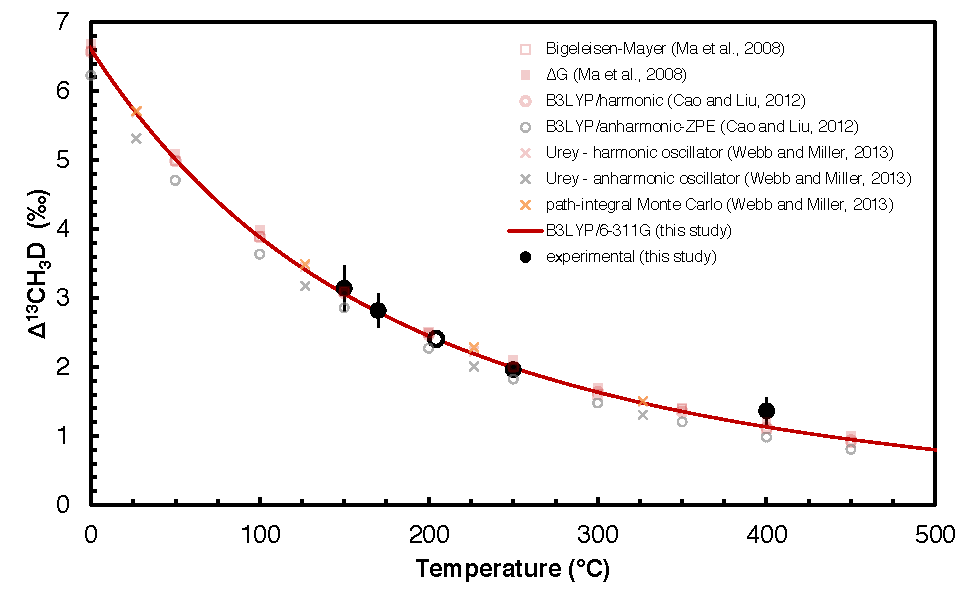
\includegraphics[width=0.8\linewidth]{figures/Fig2.S1}
	\caption[Experimental calibration of the
	Δ\textsuperscript{13}CH\textsubscript{3}D thermometer]{Experimental calibration of the
		Δ\textsuperscript{13}CH\textsubscript{3}D thermometer. Filled circles
	represent the mean Δ\textsuperscript{13}CH\textsubscript{3}D of gases
	heated at that temperature, and error bars represent 95\% confidence
	intervals calculated from a normal distribution (for the 150~°C sample,
	error bars represent the 95\% confidence interval on the measurement
	cycles in a single analysis, calculated from a \emph{t}-distribution).
	For the 250~°C point, the error bars are smaller than the symbol. The
	open circle represents our reference gas, AL1. The equilibrium curve
	(red line) was calculated following conventional equilibrium isotope
	fractionation theory under the harmonic oscillator assumption
	\parencite{Bigeleisen+Mayer_1947_JCP}; frequencies were calculated at the B3LYP level of theory
	using the 6-311G basis set as implemented in Gaussian 03 (\citeauthor{g03}).
	For comparison, results from published computational studies
	\parencite{Webb+Miller_2013_JPCA,Cao+Liu_2012_GCA,Ma++_2008_GCA} are also plotted.}
	\label{fig:2:S1}
\end{figure*}

\begin{figure*}
	\centering
	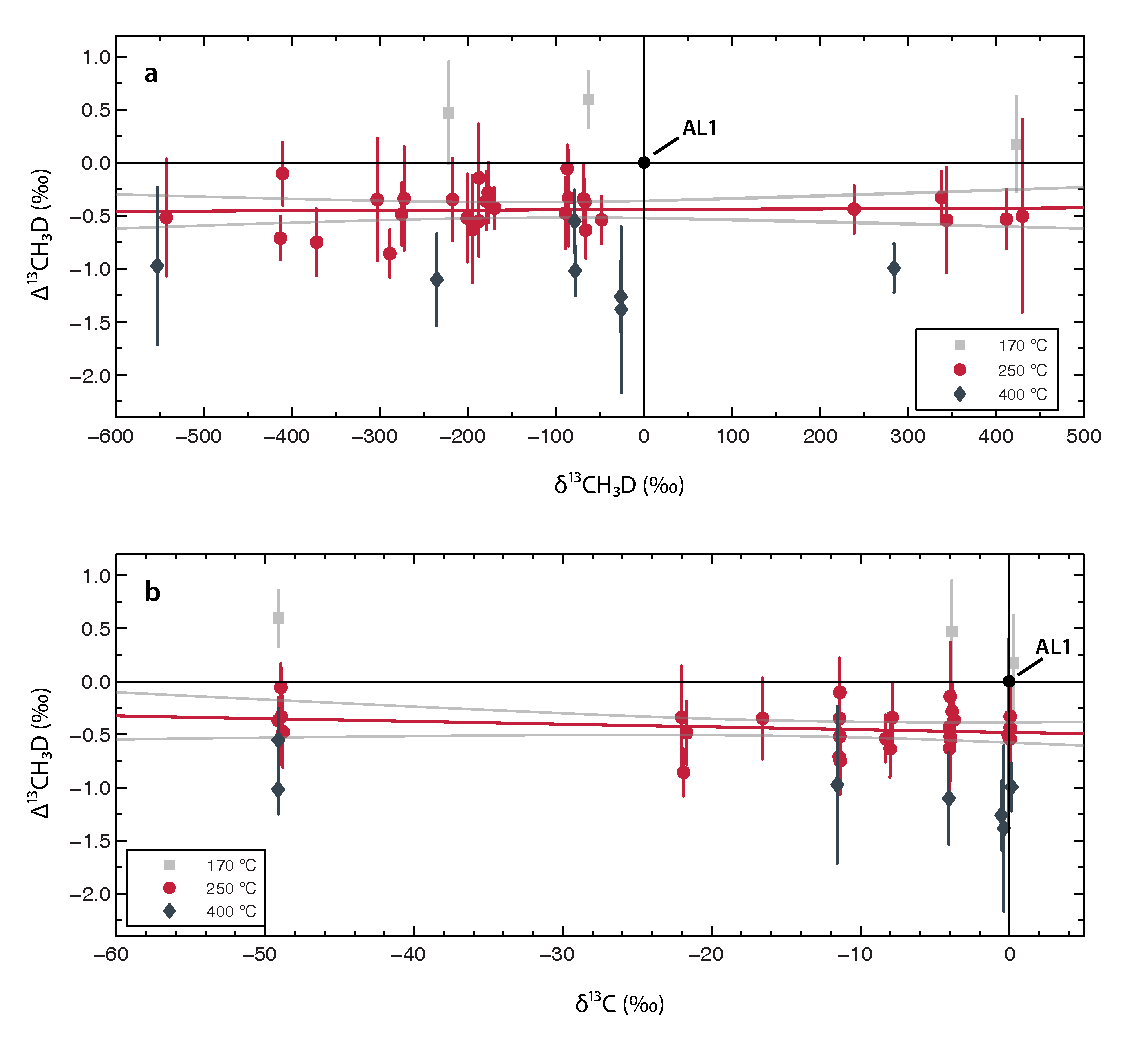
\includegraphics[width=0.85\linewidth]{figures/Fig2.S2}
	\caption[Demonstration of linearity in Δ\textsuperscript{13}CH\textsubscript{3}D over a range of bulk isotope ratios]{Demonstration of linearity in Δ\textsuperscript{13}CH\textsubscript{3}D over a range of bulk isotope ratios.  Shown are measurements of methane heated over catalyst at three
		temperatures (170, 250, 400~°C).  Solid red lines represent unweighted linear least squares
	regressions through gases equilibrated at 250~°C, and gray lines denote
	the 95\% confidence band. Error bars represent 95\% confidence intervals
	on multiple measurement cycles of a single analysis. Isotopic ratios are
	shown relative to our reference gas, AL1. Results indicate no
	significant correlation between
	Δ\textsuperscript{13}CH\textsubscript{3}D and (\textbf{A})
	δ\textsuperscript{13}CH\textsubscript{3}D over an 800‰ range (the
	variation in δ\textsuperscript{13}CH\textsubscript{3}D is driven mainly
	by differences in δD); and (\textbf{B}) δ\textsuperscript{13}C over a
	48‰ range.}
	\label{fig:2:S2}
\end{figure*}


To extract methane quantitatively from gas samples, we applied a
preparative-gas chromatography technique modified from \textcite{Alei++_1987_AtmE}. In brief, a sample is introduced into a stream of helium.
Water is removed by passing the sample through a U-trap cooled to $-$80~°C, and then CH\textsubscript{4}, air (N\textsubscript{2},
O\textsubscript{2}, Ar), CO, CO\textsubscript{2}, and
C\textsubscript{2+} are cryofocused onto a U-trap packed with activated
charcoal and held at $-$196~°C. The condensed gases are then released by
rapid heating to 120~°C, passed through a packed column (Carboxen-1000,
5$'$ × 1/8$''$, Supelco) held at 30~°C under helium flow (\textasciitilde{}25
ml/min), and monitored using thermal conductivity detection. The methane
peak is trapped on a U-trap packed with silica gel and held at $-$196~°C;
this is analogous to a ``heart-cut'' technique used previously for
preparative separation of SF\textsubscript{6} for isotopic analysis
\parencite{Ono++_2006_CG}. After elution of methane, the column is baked at 180~°C
under a reversed (backflushed) flow of helium to remove
CO\textsubscript{2} and C\textsubscript{2+}.

This sample preparation procedure induces small fractionations in
δ\textsuperscript{13}C and δD of methane of 0.09 ± 0.06‰ and 0.20 ±
0.02‰, respectively (1\emph{s}, \emph{n} = 4); these effects are minor
compared to the magnitude of δ\textsuperscript{13}C and δD variations in
nature. Critically, our procedure does not discernibly alter the
Δ\textsuperscript{13}CH\textsubscript{3}D value; the average difference
between samples treated vs.\ not treated with this procedure was $-$0.09 ±
0.16‰ (1\emph{s}, \emph{n} = 4), which is not significantly different
from zero.

\subsection{\texorpdfstring{Reporting of δ\textsuperscript{13}C and δD
		values}{Reporting of δ13C and δD
		values}}\label{reporting-of-ux3b413c-and-ux3b4d-values}

The δ\textsuperscript{13}C and δD values we report have been calibrated
relative to PDB and SMOW, respectively, by measuring samples of NGS-1
and NGS-3. These reference values for δ\textsuperscript{13}C and δD are,
respectively, $-$29.0‰ and $-$138‰ for NGS-1, and $-$72.8‰ and $-$176‰ for
NGS-3, as determined by several labs in the 1980s \parencite{Hut_1987}. Results for the calibration
samples are shown in \autoref{tab:2:S5}.

\subsection{Heated gas calibrations}\label{heated-gas-calibrations}

To confirm and extend a previously-published temperature calibration
\parencite{Ono++_2014_AC}, Pyrex tubes containing samples of methane with a range of
δ\textsuperscript{13}C ($-$82 to $-$34‰ vs.\ PDB) and δD ($-$615 to +220‰ vs.\ SMOW) were prepared. These samples were heated over Pt catalyst at
temperatures of 150, 170, 250, and 400~°C (\emph{n} = 1, 3, 28, and 7,
respectively). Gases were heated for 110 d, 73--76 d, 2--24 d, and
16--60 h, respectively, following a procedure described in 
\textcite{Ono++_2014_AC}.

When the theoretical methane equilibrium line is aligned to samples
heated at 150, 170, and 250~°C, measurements of the samples heated at
400~°C yielded slightly lower Δ\textsuperscript{13}CH\textsubscript{3}D
temperatures
($347^{+42}_{-36}$\,°C),
perhaps because quenching the reaction may take longer than the time for
exchange over catalyst at \textasciitilde{}400~°C. As a result, the data
from the 400~°C heated gases were not used in aligning the calibration
in \autoref{fig:2:S1}.

The theoretical equilibrium line we calculated agrees well with
published results from both path-integral Monte Carlo simulations
\parencite{Webb+Miller_2013_JPCA} and harmonic oscillator assumption-based approaches
\parencite{Webb+Miller_2013_JPCA,Cao+Liu_2012_GCA,Ma++_2008_GCA}. The results of results of calculations employing
an anharmonic correction, however, differ slightly from results of
models assuming harmonic-oscillator behavior \parencite[by \textasciitilde{}0.3‰
near room temperature;][]{Webb+Miller_2013_JPCA,Cao+Liu_2012_GCA}. \mrefs[]{Figure}{fig:2:S1} shows results
from recent studies comparing multiple
computational approaches for estimating the temperature-dependence of
the equilibrium Δ\textsuperscript{13}CH\textsubscript{3}D value. We note
that while the uncertainty in the theoretical curve is similar in
magnitude to our analytical uncertainty, particularly at temperatures
\textless{}100~°C, these calibration uncertainties do not affect the
conclusions drawn in this study.

\subsection{Spectroscopic procedures
}\label{spectroscopic-procedures}

Samples of purified methane were analyzed using a tunable-infrared laser
direct absorption spectrometer (Aerodyne Research, Billerica,
Massachusetts) housed at MIT as described in \textcite{Ono++_2014_AC},
with improvements described here. All measurements reported in this
paper were obtained at a nominal cell pressure of ca.\ 1.0~Torr, instead
of the 0.8~Torr used in \textcite{Ono++_2014_AC}. We have found that this
higher cell pressure gave improved measurement stability. As suggested
previously \parencite{Ono++_2014_AC}, there is a small offset in the baseline
underneath the \textsuperscript{13}CH\textsubscript{3}D absorption line,
likely due to the insufficient accuracy of the Voigt profile for
describing the contribution from tailing of adjacent
\textsuperscript{12}CH\textsubscript{4} peak. We have used all 250~°C
experiments shown in \autoref{fig:2:S2} to generate a single set of correction
factors, which show no observable drift during the time period all
measurements were made.

Long-term internal reproducibility was evaluated by repeated analysis of
methane from a commercially-sourced gas cylinder over a period of
\textgreater{}4 months, yielding precisions for δ\textsuperscript{13}C
of ±0.02‰, δD of ±0.02‰, and Δ\textsuperscript{13}CH\textsubscript{3}D
of ±0.08‰ (1\emph{s}, \emph{n} = 13). As described in \textcite{Ono++_2014_AC}, each measurement run consists of multiple acquisition
cycles (a cycle is defined as one comparison of a sample/standard pair).
The number of cycles (\emph{N}\textsubscript{cycles}) depends on sample
size, but is typically greater than 5. In this paper,
Δ\textsuperscript{13}CH\textsubscript{3}D measurements are reported as
mean ± 95\% confidence intervals (CI) on the average of all isotope
ratios obtained for each acquisition cycle over a measurement run,
calculated as: 
$ \text{95\% CI} = \mathit{tinv}\left( \alpha,\mathit{df}\right) \cdot {s\,/\sqrt{\smash[b]{N_\text{cycles}}}} $, where $ \mathit{tinv} $ is the two-tailed inverse of the Student’s \textit{t}-distribution for $ \alpha = 0.05 $ with $ N_\text{cycles} - 1 $ degrees of freedom ($ \mathit{df} $), and $ s \geq 0.27\permille$
{[}this value is the
standard deviation on measurements for which 24 or more cycles were
taken (0.27 ± 0.08‰, 1\emph{s} on 1\emph{s}, \emph{n} = 7), and thus
estimates the internal precision of the instrument{]}. The uncertainties
on Δ\textsuperscript{13}CH\textsubscript{3}D values reported for samples
in \mrefs[]{Tables}{tab:2:S1}, \ref{tab:2:S2}, and \ref{tab:2:S5} also contain the propagated uncertainty in the
Δ\textsuperscript{13}CH\textsubscript{3}D value of our methane reference
gas (AL1). Based on the calibration shown in \autoref{fig:2:S1}, we determined that
AL1 carries a Δ\textsuperscript{13}CH\textsubscript{3}D value of +2.41 ±
0.08‰ (95\% CI).



\begin{figure*}
	\centering
	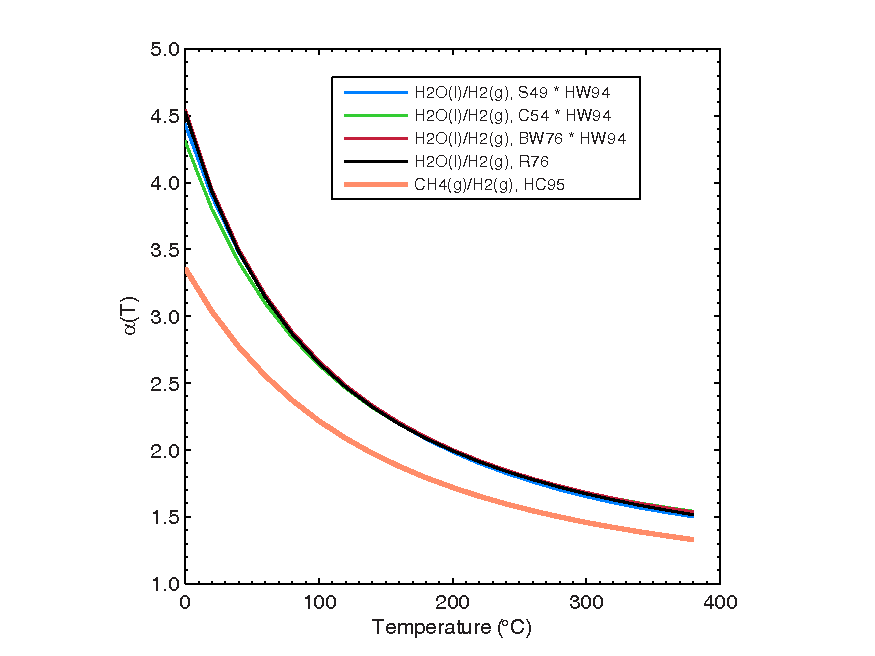
\includegraphics[width=0.8\linewidth]{figures/Fig2.S3}
	\caption[Equilibrium hydrogen isotopic fractionation factors
	for the system H\textsubscript{2}--H\textsubscript{2}O--CH\textsubscript{4}]{Equilibrium hydrogen isotopic fractionation factors
		compiled from experimental and theoretical calibrations. When
	appropriate, calibrations for
	H\textsubscript{2}O(g)/H\textsubscript{2}(g) have been converted using
	the H\textsubscript{2}O(l)/H\textsubscript{2}O(g) calibration from
	\textcite{Horita+Wesolowski_1994_GCA} to derive
	H\textsubscript{2}O(l)/H\textsubscript{2}(g) calibrations. 
	HW94, \textcite{Horita+Wesolowski_1994_GCA}; 
	S49, \textcite{Suess_1949}; 
	C54, \textcite{Cerrai++_1954}; 
	BW76, \textcite{Bardo+Wolfsberg_1976_JPC}; 
	R76, \textcite{Rolston++_1976_JPC};
	HC95, \textcite{Horibe+Craig_1995_GCA}. For any temperature,
	the CH\textsubscript{4}(g)/H\textsubscript{2}O(l) equilibrium
	composition is the ratio of the
	CH\textsubscript{4}(g)/H\textsubscript{2}(g) line (HC95) to a
	H\textsubscript{2}O(l)/H\textsubscript{2}(g) line.}
	\label{fig:2:S3}
\end{figure*}

To enable analysis of small (ca.\ 1~cm\textsuperscript{3} STP) methane
samples, we have developed a cold trap system to recover and recycle
methane samples for re-analysis. In the current study, the only sample
for which this recycling method was used was ``Sally-1'', a sample from
a bovine rumen (\autoref{tab:2:S1}).


\begin{table}\centering
	
	\caption[Isotope fractionation factors used
in model calculations for microbial methane]{Isotope fractionation factors (input parameters) used
		in model calculations for microbial methane generated at 20~°C. A
		detailed description of the model setup and explanation of choices of
		fractionation factors is given in \autoref{model-of-isotopologue-systematics-during-microbial-methanogenesis}.}
	\label{tab:2:S3}
	
	\begin{threeparttable}

		
		\small
		\begin{tabular}{llll}
			\toprule
			& forward & backward & equilibrium\tabularnewline
			\midrule
			\textsuperscript{13}C/\textsuperscript{12}C isotope effect
			(\textsuperscript{13}$\alpha$) & 0.9600* & 0.9771\textsuperscript{†} &
			0.9824\textsuperscript{‡}\tabularnewline
			D/H primary isotope effect (\textsuperscript{2}$\alpha$\textsubscript{p}) &
			0.600 to 0.750\textsuperscript{§} & 0.751 to 0.939\textsuperscript{\#} &
			0.7989\textsuperscript{\textbar{}\textbar{}}\tabularnewline
			D/H secondary isotope effect (\textsuperscript{2}$\alpha$\textsubscript{s}) &
			0.8400\textsuperscript{¶} & 0.8400\textsuperscript{¶} &
			1.0000\textsuperscript{¶}\tabularnewline
			\textsuperscript{13}C-D clumped isotope effect ($\gamma$) & 0.9987 or 0.9965**
			& 0.9928 or 0.9907\textsuperscript{††} &
			1.0059\textsuperscript{‡‡}\tabularnewline
			\bottomrule
		\end{tabular}
		
		\begin{tablenotes}
			\item * From \textcite{Scheller++_2013_JACS_KIE} for the reduction of methyl-coenzyme
			M.
			
			\item † Internally-consistent value. For comparison, \textcite{Hermes++_1984_Bc}
			 reported 0.96 for formate dehydrogenase, and \textcite{Scharschmidt++_1984_Bc} reported 0.979 for alcohol dehydrogenase.
			
			\item ‡ From \textcite{Horita_2001_GCA}, who determined
			\textsuperscript{13}$\alpha$\textsubscript{\ce{CH4}/\ce{CO2}} = 0.932 at 20~°C; this
			reported value is equal to 0.9824 taken to the power of 4.
			
			\item § Free parameter. The range of values used here are similar to those
			reported for \emph{in vitro} studies of methyl-coenzyme M reductase
			(0.63 to 1.0) \parencite{Scheller++_2013_JACS_KIE} and from experimental cultures of methanogens
			(0.70 to 0.86) \parencite{Valentine++_2004_GCA}.
			
			\item \# Internally-consistent value. For comparison, \textcite{Scheller++_2013_JACS_KIE} 
			determined a value of 0.41 ± 0.04 (they reported a primary isotope effect of $k_\mathrm{H}/k_\mathrm{D}$ = 2.44 ± 0.22 for the activation of methane; the reciprocal of this value is \textsuperscript{2}$\alpha$\textsubscript{p}).
			
			\item \textbar{}\textbar{} From the value given by
			\textcite{Horibe+Craig_1995_GCA} for the equilibrium D/H fractionation factor between
			H\textsubscript{2}O(l) and CH\textsubscript{4}(g) at 20~°C.
			
			\item ¶ From \textcite{Scheller++_2013_JACS_KIE} for the reduction of methyl-CoM.  For comparison, \textcite{Roston+Kohen_2010_PNAS} 
			reported secondary D/H isotope effects associated with the reduction of an aldehyde by alcohol dehydrogenase of 0.94 for the forward reaction and 0.81 for the reverse reaction. 
			
			\item ** To fit the lowest Δ\textsuperscript{13}CH\textsubscript{3}D values we
			have observed in methanogen culture experiments (0.9987, corresponding
			to Δ\textsuperscript{13}CH\textsubscript{3}D = $-$1.3‰, \autoref{tab:2:S2}) or in
			nature (0.9965, corresponding to
			Δ\textsuperscript{13}CH\textsubscript{3}D = $-$3.5‰, \autoref{tab:2:S1}).
			Calculations for the fields shown in \mrefs[]{Figs.}{fig:2:2} and~\ref{fig:2:4} use the latter
			values. See \autoref{model-of-isotopologue-systematics-during-microbial-methanogenesis} for explanation of choice, and
			\autoref{fig:2:S5} for comparison of model results using the two different values.
			
			\item †† Internally-consistent value. For comparison, \textcite{Hermes++_1984_Bc}
			reported 0.999 for formate dehydrogenase, and \textcite{Scharschmidt++_1984_Bc} reported 0.995 for alcohol dehydrogenase.
			
			\item ‡‡ Computed equilibrium Δ\textsuperscript{13}CH\textsubscript{3}D value
			at 20~°C (\autoref{fig:2:S1}).
		\end{tablenotes}

	\end{threeparttable}
\end{table}

\begin{table}\centering
	\begin{threeparttable}
		\caption[C\textsubscript{1}/C\textsubscript{2}, δD\textsubscript{water}, current environmental temperatures, and {[}H\textsubscript{2}{]} for sites studied]{Methane/ethane ratio, hydrogen isotopic composition of
			water, current environmental temperatures, and concentration of
			dissolved H\textsubscript{2} for sites studied. References are provided
			for previously-published descriptions of the field site; n.d., not
			determined.}
		\label{tab:2:S4}
		
		\begin{tabular}{l r r@{\hspace{0.2em}}l r@{\hspace{0.2em}}l r l}
			\toprule
			Location & C\textsubscript{1}/C\textsubscript{2}
			\textsuperscript{\textbar{}\textbar{}} & \multicolumn{2}{c}{δD\textsubscript{water}
			(‰)\textsuperscript{¶}} & \multicolumn{2}{c}{\textit{T} (°C)\textsuperscript{\#}} & {[}H\textsubscript{2}{]}** & 
			Data Sources\tabularnewline
			\midrule
			Bovine rumen, Pennsylvania, USA & n.d. & \textbf{$-$32} & ±
			10 & \textbf{39} & ± 2 & \emph{0.1--50 µM} & this
			study*\textsuperscript{,‡}, {[}1{]}\tabularnewline
			Northern Cascadia Margin sediments & \textgreater{}1000 &
			\emph{\textbf{+5}} & \emph{± 10} & \textbf{3--17} & & \emph{2--60 nM} &
			{[}2{]}\tabularnewline
			Powder River Basin, Montana, USA & \textgreater{}1000 & \textbf{$-$136} &
			± 5 & \textbf{18} & ± 2 & n.d. & this
			study\textsuperscript{§}\tabularnewline
			Cedar swamp, Massachusetts, USA & n.d. &
			\textbf{$-$21} & ± 10 & \emph{\textbf{16}} & \emph{± 5} & n.d. & this
			study\textsuperscript{‡}\tabularnewline
			Upper Mystic Lake, Mass., USA & n.d. & \textbf{$-$39} & ± 10 &
			\textbf{4} & ± 2 & n.d. & this study\textsuperscript{‡}\tabularnewline
			Lower Mystic Lake, Mass., USA & \textgreater{}1000 &
			\textbf{$-$41} & ± 10\textsuperscript{††} & \textbf{6} & ± 2 & n.d. & this
			study\textsuperscript{‡}\tabularnewline
			The Cedars, California, USA & \textgreater{}350 & \emph{\textbf{$-$37}} &
			\emph{± 10} & \emph{\textbf{17}} & \emph{± 1} & \emph{120, 310 µM} &
			{[}3{]}\tabularnewline
			CROMO, California, USA &
			\textgreater{}350 & \textbf{$-$33} & ± 10\textsuperscript{††} & \textbf{16} & ± 4 & 60--130 nM
			& this study\textsuperscript{†,‡}\tabularnewline
			Kidd Creek Mine, Ontario, Canada & 5.9--14 & \textbf{$-$34} & ± 6
			& \textbf{30} & ± 2 & \emph{0.8--8 mM} & {[}4{]}\tabularnewline
			Rebecca's Roost vent, Guaymas Basin & 140 &
			\emph{\textbf{+4}} & \emph{± 2} & \textbf{299} & ± 5 & 3.3 mM &
			{[}5{]}\tabularnewline
			Marcellus Fm., Penn., USA & 45 & \emph{\textbf{$-$44}} &
			\emph{± 10} & \textbf{51} & ± 10 & n.d. & {[}6{]}\tabularnewline
			Utica Fm., Penn., USA & 84 & \emph{\textbf{$-$40}} &
			\emph{± 15} & \textbf{93} & ± 10 & n.d. & {[}7{]}\tabularnewline
			\bottomrule
		\end{tabular}

		\begin{tablenotes}\small

			\item * H\textsubscript{2} concentrations were determined using gas
			chromatography with thermal conductivity detection at MIT. Analytical
			reproducibility is typically ±5\%.
			
			\item † H\textsubscript{2} concentrations were determined using a reduced
			gas analyzer gas chromatograph at NASA Ames \parencite{Crespo-Medina++_2014_FMicro}.
			
			\item ‡ The δD\textsubscript{water} was measured at the Boston
			University Stable Isotope Laboratory using high-temperature conversion
			gas chromatography isotope-ratio mass spectrometry. External
			reproducibility on replicate analyses of samples was ± 1--3‰ (1\emph{s},
			\emph{n} = 3--4), with the exception of cow rumen fluid (±8‰,
			1\emph{s}).
			
			\item § The δD\textsubscript{water} values were measured at the University of
			Arizona Environmental Geochemistry Laboratory via isotope-ratio mass
			spectrometry.
			
			\item \textbar{}\textbar{} Unless otherwise indicated, the
			C\textsubscript{1}/C\textsubscript{2} ratio (i.e., the ratio of the
			concentration of methane to that of ethane in a gas sample) was
			determined using gas chromatography with flame-ionization detection at
			MIT.
			
			\item ¶ The δD\textsubscript{water} values are reported with respect to the
			VSMOW scale.
			
			\item \# At some sites ambient temperatures were not directly measured
			(\emph{in italics}) and therefore were estimated; reasonable
			uncertainties on those estimates are given. At all other sites
			temperatures were measured \emph{in situ}.
			
			\item ** Dissolved \ce{H2} concentrations estimated from the literature are \emph{in italics}.
			
			\item †† At Lower Mystic Lake and CROMO, the waters in which methane was generated may have δD\textsubscript{water} values different from those in the water samples measured because of migration (see \autoref{field-notes-and-thoughts-on-selected-localities}).
			
			\item {[}1{]} Range of {[}H\textsubscript{2}{]} from \textcite{Janssen_2010_AFST}.
			
			\item {[}2{]} For the Northern Cascadia Margin samples, an average D/H ratio
			of marine sediment porewater \parencite[+5‰,][]{Friedman+Hardcastle_1988_JGR} is assumed. The
			natural variability of ±10‰ is taken as the uncertainty of this
			estimate. Downhole temperature measurements from Expedition 311 have
			been reported \parencite{IODP_x311_Proceedings}. Concentrations of H\textsubscript{2} were
			assumed to be within the range of 2--60 nM, which is typical of marine
			sediments \parencite{Lin++_2012_GCA}. The C\textsubscript{1}/C\textsubscript{2} data
			are from \textcite{Pohlman++_2009_EPSL}.
			
			\item {[}3{]} The {[}H\textsubscript{2}{]}, δD­\textsubscript{water} and
			temperature data are from \textcite{Morrill++_2013_GCA}. An uncertainty of
			±10‰ is applied to δD\textsubscript{water} to account for potential
			interannual variability. Dissolved {[}H\textsubscript{2}{]} was
			estimated from the H\textsubscript{2} mole \% in the gas phase,
			assuming equilibrium between gas bubbles and water at atmospheric pressure.
			
			\item {[}4{]} Dissolved {[}H\textsubscript{2}{]} for Kidd Creek fluids was
			estimated using gas/water flow rate data from \textcite{Holland++_2013_N}
			and gas-phase H\textsubscript{2} concentrations from \textcite{SherwoodLollar++_2008_GCA}, and assuming that all dissolved H\textsubscript{2} had
			completely partitioned into the gas phase prior to sampling. The
			C\textsubscript{1}/C\textsubscript{2} data are from \textcite{SherwoodLollar++_2002_N}.
			
			\item {[}5{]} Measured vent temperature and {[}H\textsubscript{2}{]} are from \textcite{Reeves++_2014_PNAS}, and δD\textsubscript{water} was assumed based on \textcite{Shanks++_1995_AGU-GM}.
			
			\item {[}6{]} The δD\textsubscript{water} values for formation water from the
			Marcellus Fm.\ in Pennsylvania are estimated from \textcite{Rowan++_2014_AAPGB}. Uncertainty on reservoir temperature is estimated at ±10~°C.
			
			\item {[}7{]} The δD\textsubscript{water} values for formation water from the
			Utica Fm.\ are estimated using data for Appalachian Basin brines from
			pre-Middle Devonian units presented in \textcite{Warner++_2012_PNAS}.
			Uncertainty on reservoir temperature is estimated at ±10~°C.


		\end{tablenotes}

	\end{threeparttable}
\end{table}




\subsection{Model of isotopologue systematics during microbial
	methanogenesis
}\label{model-of-isotopologue-systematics-during-microbial-methanogenesis}



\begin{figure*}
	\centering
	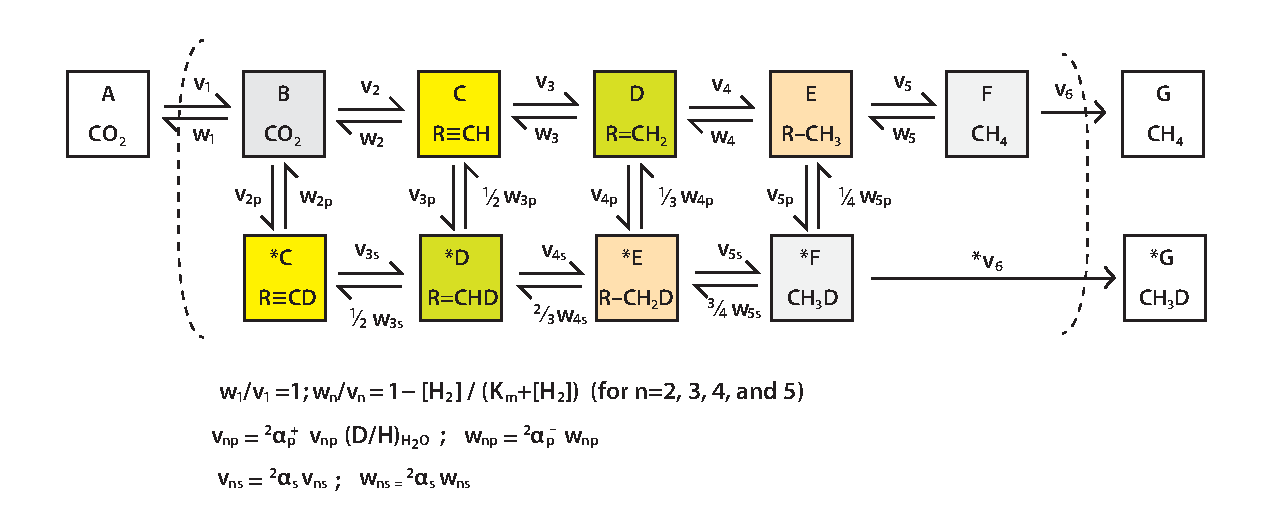
\includegraphics[width=0.9\linewidth]{figures/Fig2.S4}
	\caption[Schematic of the model of deuterium substitution during
	microbial methanogenesis from CO\textsubscript{2}]{Schematic of the model of deuterium substitution during
		microbial methanogenesis from CO\textsubscript{2}. Boxes represent
	pools of cellular carbon involved in the methanogenic pathway, and the
	asterisk represents a compound containing a deuterium substitution.
	Forward flows are represented by \emph{v}, and backwards flows are
	represented by \emph{w}. The model setup is similar in concept to
	previously published models for microbial sulfate reduction \parencite{Rees_1973_GCA,Brunner+Bernasconi_2005_GCA,Farquhar++_2007_GCA}.}
	\label{fig:2:S4}
\end{figure*}



\begin{SCfigure*}
	\centering
	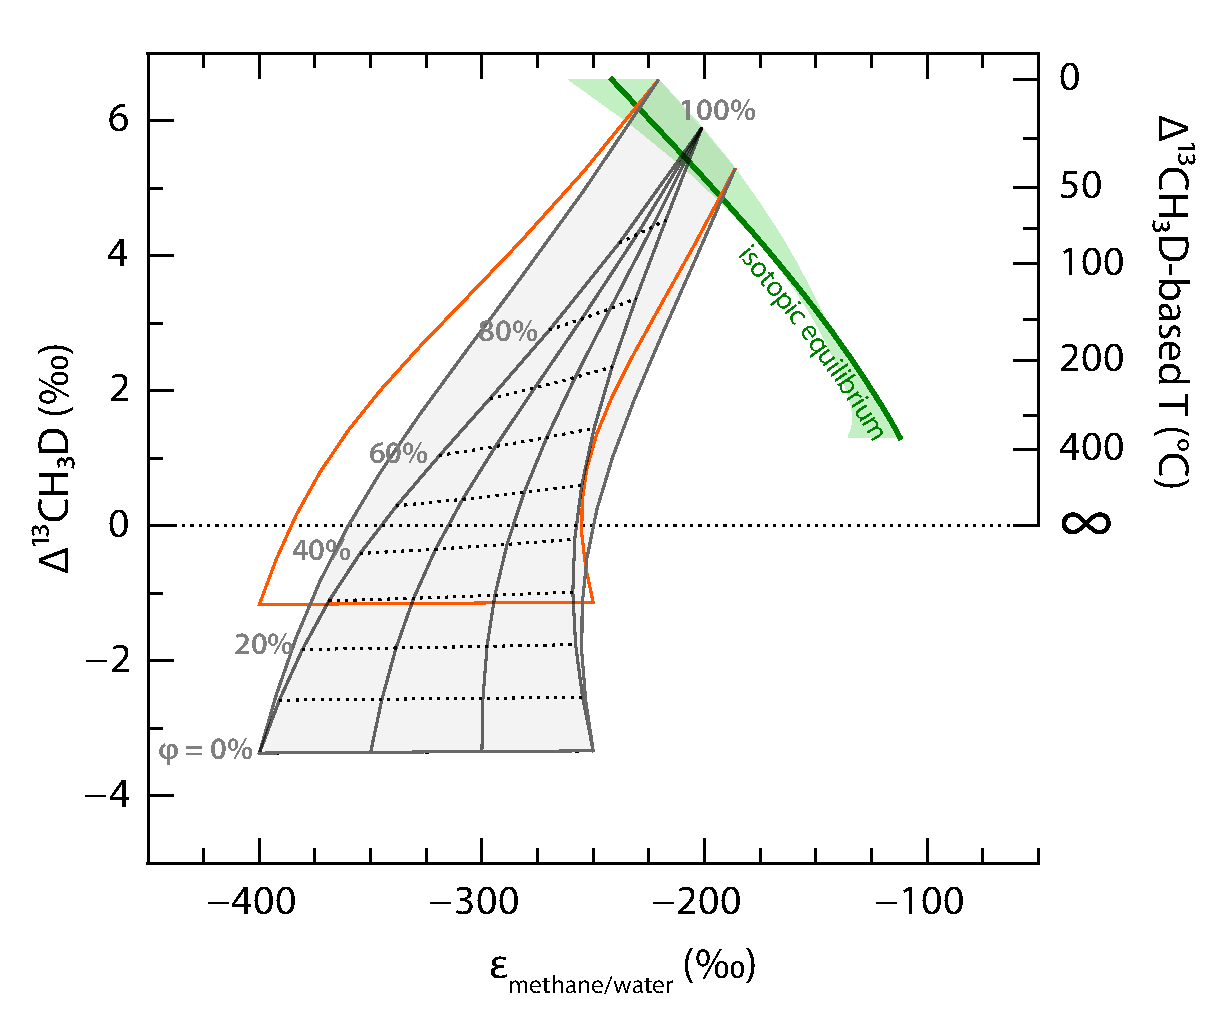
\includegraphics[width=0.5\linewidth]{figures/Fig2.S5}
	\caption[Dependence of model predictions on reversibility and fractionation
	factors]{Dependence of the modeled isotopic composition of microbial
		methane on the degree of reversibility and isotope fractionation
		factors. Orange and gray fields represent model output assuming a
		kinetic endmembers of $-$1.3‰ and $-$3.5‰, respectively (\autoref{tab:2:S3}). Inner
		solid gray lines represent model trajectories for 20~°C assuming
		different values for the D/H primary intrinsic isotope effect (\autoref{tab:2:S3}). Subhorizontal tie lines connect points of equal reversibility ($\varphi$).
		Outer solid lines represent bounding model trajectories calculated for 0
		and 40~°C.}
	\label{fig:2:S5}
\end{SCfigure*}

A mathematical model was constructed to describe isotopologue
compositions of methane produced from microbial methanogenesis (\autoref{fig:2:S4}). To allow for the use of data from studies on experimental and
natural systems as input parameters, our model simplifies the
representation of the biochemistry involved in the microbial generation
of methane, and only considers the production of methane via reduction
of CO\textsubscript{2}.

The model describes methanogenesis in six steps, and using an assumption
of steady-state intermediate compositions, solves for the abundances of
\textsuperscript{13}C- and D-substituted isotopologues of product
CH\textsubscript{4} and of four intermediate species (\autoref{fig:2:S4}). The
first step (1) is the uptake of CO\textsubscript{2} into the cell, and
the last step (6) is export of CH\textsubscript{4} out of the cell; we
assume that neither of these steps discriminates against isotopes or
between isotopologues. Inside the cell, the reduction of
CO\textsubscript{2} to CH\textsubscript{4} is treated in four steps
(steps \#2--5), where each step corresponds to the addition of one
hydrogen \parencite{Thauer_1998_M}.

The main variable input in our model is metabolic reversibility, which
is defined as the ratio of backwards to forwards fluxes
($\varphi_n = w_n \big/ v_n$) through an enzymatically-mediated reaction
sequence \parencite{Rees_1973_GCA,Hayes_2001_RiMG}. The reversibility is constrained by two
end-members, which represent fully-irreversible ($\varphi$ = 0; fully-kinetic)
and fully-reversible ($\varphi$ → 1; equilibrium) conditions. We parameterize the
reversibility as a simple function of H\textsubscript{2} concentration
by assuming Michaelis-Menten kinetics for each H-addition step:
\begin{equation}\label{eqn:phirevH2}
\varphi_n = 1 - \frac{[\ce{H2}]}{K_\text{M}+[\ce{H2}]}
\end{equation}
where \emph{n} represents the step number and \emph{K}\textsubscript{M}
is the effective half-saturation constant for H\textsubscript{2}
(assumed identical for steps 2--5). In our model, $\varphi$\textsubscript{1} is
set at 1 (i.e., CO\textsubscript{2} uptake is fully reversible).

Under an assumption of steady-state concentrations of intermediates, all
fluxes for the \textsuperscript{12}CH isotopologues are dependent upon
the methane formation rate (\emph{v}\textsubscript{6}, in e.g., mol
cell\textsuperscript{$-1$} s\textsuperscript{$-1$}) by:
\begin{equation}\label{eqn:methaneformationrate}
v_n=v_6/(1-\varphi_n ) \text{, and } w_n= \varphi_n v_6/(1-\varphi_n )
\end{equation}

A series of continuity equations can be written for each \textsuperscript{13}C-substituted isotopologue.  For example: 
%\begin{widetext}
\begin{equation}\label{eqn:continuityequations}
\frac{d^{13}\mathbf{D}}{dt} = {}_{\ }^{13}\alpha_{3}^{+} \cdot  v_{3} \cdot  {_{\ }^{13}r}_{\mathbf{C}} - \left(_{\ }^{13}\alpha_{4}^{+} \cdot v_{4} + {}_{\ }^{13}\alpha_{3}^{-} \cdot  w_{3} \right) \cdot  {_{\ }^{13}r}_{\mathbf{D}} + {}_{\ }^{13}\alpha_{4}^{-} \cdot  w_{4} \cdot {}_{\ }^{13}r_{\mathbf{E}}
\end{equation}
%\end{widetext}

Here, \textsuperscript{13}\textbf{D} is the abundance of
\textsuperscript{13}C-substituted isotopologues for the pool \textbf{D}
(i.e., R=CH\textsubscript{2}; \autoref{fig:2:S4}), and
\textsuperscript{13}\emph{r}\textbf{\textsubscript{X}} is the
isotopologue ratio of the pool \textbf{X} (where \textbf{X} =
\textbf{A}, \textbf{B}, \ldots{}, \textbf{F}), and
\textsuperscript{13}$\alpha$\emph{\textsubscript{n}}\textsuperscript{+} and
\textsuperscript{13}$\alpha$\emph{\textsubscript{n}}\textsuperscript{$-$} are the
\textsuperscript{13}C/\textsuperscript{12}C kinetic isotope effects
associated with the forward and backward reactions, respectively. There
are a total of five continuity equations for pools
\textsuperscript{13}\textbf{B}, \textsuperscript{13}\textbf{C},
\textsuperscript{13}\textbf{D}, \textsuperscript{13}\textbf{E}, and
\textsuperscript{13}\textbf{F}. Under an assumption of steady-state
concentrations of intermediate species (i.e.,
\emph{d}\textsuperscript{13}\textbf{X}/\emph{dt} = 0), we solve for the
ratios of \textsuperscript{13}C-containing to
\textsuperscript{12}C-containing isotopologues in the product methane
(\textbf{F}; i.e.,
\textsuperscript{13}CH\textsubscript{4}/\textsuperscript{12}CH\textsubscript{4})
and in the intermediates (\textbf{B}, \textbf{C}, \textbf{D}, and
\textbf{E}). The \textsuperscript{13}C/\textsuperscript{12}C ratio of
CO\textsubscript{2} (i.e., \emph{r}\textbf{\textsubscript{A}}) is
assigned.

For the deuterated isotopologues, the continuity equations account for
both primary isotope effects (describing the rates at which C--D bonds
are formed or broken relative to C--\textsuperscript{1}H bonds; fluxes
shown vertically in \autoref{fig:2:S4}) and secondary isotope effects (describing
the change in reaction rate resulting from D substitution at a site
\emph{adjacent} to that which is site of an
\textsuperscript{1}H-addition or abstraction reaction; fluxes shown
horizontally in \autoref{fig:2:S4}). For example for reservoir \textbf{D}, the continuity
equation for the D-substituted isotopologue (i.e., R=CH\textsubscript{2}
or R=CHD) is:
%\begin{widetext}
\begin{equation}\label{eqn:continuityeqnexampledeuterated}
\begin{split}
\frac{d^{2}\mathbf{D}}{{dt}} = {}_{\ }^{\ }{_{\ }^{2}\alpha_{3p}^{+} \cdot v_{3} \cdot {_{\ }^{2}r}_{\mathbf{H}} &+ {}_{\ }^{2}\alpha_{3s}^{+} \cdot v_{3} \cdot {_{\ }^{2}r}_{\mathbf{C}} \\
	&- \left( \tfrac{1}{2} \cdot {_{\ }^{2}\alpha}_{3s}^{-} \cdot w_{3} + \tfrac{1}{2} \cdot {}_{\ }^{2}\alpha_{3p}^{-} \cdot w_{3} + {}_{\ }^{2}\alpha_{4s}^{-} \cdot v_{4} \right) \cdot {_{\ }^{2}r}_{\mathbf{D}} \\&+ \tfrac{2}{3} \cdot {}_{\ }^{2}\alpha_{4s}^{-} \cdot w_{4} \cdot {_{\ }^{2}r_{\mathbf{E}}}_{\ }}
\end{split}
\end{equation}
%\end{widetext}

Here, \textsuperscript{2}$\alpha$\textsubscript{\emph{n}p} and
\textsuperscript{2}$\alpha$\textsubscript{\emph{n}s} are primary and secondary
deuterium isotope effects, 
\textsuperscript{2}\emph{r}\textsubscript{\textbf{X}} are D-isotopologue
ratios for reservoir \textbf{X}, and 
\textsuperscript{2}\emph{r}\textsubscript{\textbf{H}} is the D/H ratio of the
hydrogen source (i.e., cellular water). The stoichiometric factor
corresponds to the probability of a primary versus secondary
isotope-sensitive reaction occurring (in this case, there is a $\sfrac{2}{3}$ chance
of removing H from R--CH\textsubscript{2}D). Again, there are five linear
equations to be solved simultaneously. Conversion between isotopologue
ratios and isotope ratios requires consideration of reaction
stoichiometry. For example,
\begin{equation}
{}_{\ }^{2}r_\mathbf{D} = \frac{\left\lbrack \mathrm{R}{=}\mathrm{\text{CHD}} \right\rbrack}{\left\lbrack \mathrm{R}{=}\mathrm{C}\mathrm{H}_{\mathrm{2}} \right\rbrack} = 2\left( \frac{\mathrm{D}}{\mathrm{H}} \right)_{\mathrm{R}{=}\mathrm{C}\mathrm{H}_{\mathrm{2}}}\ 
\end{equation}

Clumped isotopologue ratios (e.g.,
{[}R=\textsuperscript{13}CHD{]}/{[}R=\textsuperscript{12}CH\textsubscript{2}{]})
can be solved for in a manner similar to that used for D-substituted
isotopologues above.

For simplicity, primary ($\alpha$\textsubscript{p}) and secondary
($\alpha$\textsubscript{s}) kinetic isotope fractionation factors for the four
H-addition steps are assumed to be identical at a given temperature
(fractionation factors calculated for a model temperature of 20~°C are
shown in \autoref{tab:2:S3}). The intrinsic (kinetic/forward)
\textsuperscript{13}C/\textsuperscript{12}C and D/H fractionation
factors are estimated from \emph{in vitro} and culture studies \parencite{Valentine++_2004_GCA,Hermes++_1984_Bc,Roston+Kohen_2010_PNAS,Scharschmidt++_1984_Bc,Scheller++_2013_JACS_KIE}. The intrinsic \textsuperscript{13}CD
fractionation factor ($\gamma$, where \textsuperscript{13D}$\alpha$ = $\gamma$ ·
\textsuperscript{13}$\alpha$ · \textsuperscript{2}$\alpha$) is taken to have the value
required to generate a Δ\textsuperscript{13}CH\textsubscript{3}D
signature of either $-$1.3‰ or $-$3.5‰ under fully-kinetic conditions (\nameref{main-text} and \autoref{tab:2:S3}). The \textsuperscript{13}C/\textsuperscript{12}C,
D/H, and \textsuperscript{13}CH\textsubscript{3}D equilibrium isotope
fractionation factors are based on experimental and/or theoretical
calibrations (\mrefs[]{Figs.}{fig:2:2}, \ref{fig:2:S1}, and \ref{fig:2:S3}) \parencite{Ono++_2014_AC,Horibe+Craig_1995_GCA,Cerrai++_1954,Horita_2001_GCA}. The intrinsic fractionation factors for the
reverse reactions ($\alpha$\textsuperscript{$-$}, \autoref{tab:2:S3}) are constrained by
the requirement for consistency among equilibrium ($\alpha$\textsubscript{eq}),
forward ($\alpha$\textsuperscript{+}), and reverse reactions (i.e.,
$\alpha$\textsubscript{eq} = $\alpha$\textsuperscript{$-$}/$\alpha$\textsuperscript{+}). We
note that varying the secondary isotope effect ($\alpha$\textsubscript{s},
assumed to be 0.84 in either direction, for all steps) changes the
curvature of the modeled microbial trajectories, but does not change the
endmember $\varepsilon$\textsubscript{methane/water} values (which are set by the
primary D/H isotope effect).

We initiated the model calculations at temperatures of 0, 20, and 40~°C.
These temperatures bracket the range of known or inferred environmental
temperatures at which the microbial methane samples we studied were
generated (\autoref{tab:2:S4}). The predicted isotopic compositions for microbial
methane generated between 0 and 40~°C are shown in \mrefs[]{Figs.}{fig:2:2} and \ref{fig:2:4}.

\begin{table}\centering
	
	\caption[Results of isotopic measurements of methane
	in samples of natural gas standards]{Results of isotopic measurements of methane
		in samples of natural gas standards NGS-1 and NGS-3. Uncertainties
		reported are 95\% confidence intervals over all measurement cycles for a
		single analysis as described in \autoref{spectroscopic-procedures}. Values for
		δ\textsuperscript{13}C, δD, and
		Δ\textsuperscript{13}CH\textsubscript{3}D are reported relative to PDB,
		SMOW, and the stochastic distribution, respectively.}
	\label{tab:2:S5}

	\begin{threeparttable}
		
		\begin{tabular}{l r@{\hspace{0.2em}}l r@{\hspace{0.2em}}l >{\raggedleft\arraybackslash}p{2.5em}@{\hspace{0.2em}}l r@{\hspace{0.2em}}l}
			% This notation >{\raggedleft\arraybackslash}p{5em} is for padding the left side so that multicolumn doesn't expand extra space on the right column of the multicolumn{2}{c}. http://stackoverflow.com/a/25690685
			\toprule
			Sample Name & \multicolumn{2}{c}{δ\textsuperscript{13}C (‰)} & \multicolumn{2}{c}{δD (‰)} &
			\multicolumn{2}{c}{Δ\textsuperscript{13}CH\textsubscript{3}D (‰)} & \multicolumn{2}{c}{\textit{T}\textsubscript{13D}
				(°C)}\tabularnewline
			\midrule
			NGS-1 & \textbf{$-$28.73} & ± 0.05  & \textbf{$-$137.47} & ± 0.05  &
			 \textbf{2.61} & ± 0.29  & \textbf{186} & +28/$-$24 \tabularnewline
			& \textbf{$-$28.79} & ± 0.07  & \textbf{$-$137.69} & ± 0.07  &
			\textbf{2.53} & ± 0.29  & \textbf{193} & +29/$-$25 \tabularnewline
			& \textbf{$-$28.91} & ± 0.05  & \textbf{$-$138.07} & ± 0.05  &
			\textbf{2.62} & ± 0.24  & \textbf{185} & +22/$-$19 \tabularnewline
			\midrule
			NGS-3 & \textbf{$-$72.82} & ± 0.06  & \textbf{$-$176.09} & ± 0.06  &
			\textbf{5.08} & ± 0.26  & \textbf{48} & +10/$-$9 \tabularnewline
			& \textbf{$-$72.71} & ± 0.05  & \textbf{$-$175.82} & ± 0.05  &
			\textbf{5.18} & ± 0.26  & \textbf{44} & +10/$-$9 \tabularnewline
			NGS-3 + 150ml air * & \textbf{$-$72.99} & ± 0.06  & \textbf{$-$176.21} & ±
			0.06  & \textbf{5.14} & ± 0.49  & \textbf{45} & +19/$-$17
			\tabularnewline
			\bottomrule
		\end{tabular}
	
		\begin{tablenotes}
			\item * This sample was a subsample of NGS-3 that was
			intentionally-contaminated with 150 ml of air, to check for artifacts
			introduced from sample preparation and analysis of samples containing
			large quantities of air. No significant difference was found compared to
			subsamples of NGS-3 that were not contaminated with air.	
		\end{tablenotes}
	
	\end{threeparttable}
\end{table}





\section{Supplementary Text}\label{supplementary-text}

\subsection{Evaluation of alternative mechanisms for isotopic
	disequilibria in microbial methane
}\label{evaluation-of-alternative-mechanisms-for-isotopic-disequilibria-in-microbial-methane}

There are several potential alternative mechanisms for the observed
isotopic disequilibria in microbial methane shown in \autoref{fig:2:2}. It is
conceivable that these signals are due to mixing of multiple methane
sources with differing δ\textsuperscript{13}C and δD values, as
Δ\textsuperscript{13}CH\textsubscript{3}D changes non-linearly upon
mixing. The magnitude of non-linearity in the mixing depends on the
difference in both δ\textsuperscript{13}C and δD values of the
endmembers. It can be shown, using a Taylor-series expansion
\parencite{Ono++_2006_GCA}, that two-component mixing of endmembers (A \& B) produces a
mixture with a Δ\textsuperscript{13}CH\textsubscript{3}D value of:
%\begin{widetext}
\begin{equation}\label{eqn:2:mixing}
\begin{split}
{{\Delta}^{{13}}\mathrm{\text{CH}}_{{3}}\mathrm{D}}_{\mathrm{\text{mixture}}} \approx {f}_{\mathrm{A}} \cdot {\Delta}^{{13}}\mathrm{\text{CH}}_{{3}}\mathrm{D}_{\mathrm{A}} &+ \left( {1 -}{f}_{\mathrm{A}} \right)\cdot{\Delta}^{{13}}\mathrm{\text{CH}}_{{3}}\mathrm{D}_{\mathrm{B}} \\
&+ {f}_{\mathrm{A}}\cdot\left( {1 -}{f}_{\mathrm{A}} \right)\cdot\left( {\updelta}^{{13}}\mathrm{C}_{\mathrm{A}}{-}{\updelta}^{{13}}\mathrm{C}_{\mathrm{B}} \right)\cdot\left( {\updelta}\mathrm{D}_{\mathrm{A}}{-}{\updelta}\mathrm{D}_{\mathrm{B}} \right)
\end{split}
\end{equation}
%\end{widetext}
where $f_\text{A}$ represents the fractional contribution
from endmember A. Accordingly, the observed \textasciitilde{}6‰ negative
bias in Δ\textsuperscript{13}CH\textsubscript{3}D values (from that
expected for equilibrium at 0--40~°C, \autoref{fig:2:1}) requires mixing of two
methane sources with δ\textsuperscript{13}C and δD values that differ by
±60‰ and $\mp$400‰, respectively; gases with these isotopic compositions are
unlikely to co-occur in the environments we studied \parencite{Whiticar_1990_OG}.

Alternatively, under a commonly-used classification based on
δ\textsuperscript{13}C and δD values \parencite{Whiticar_1999_CG}, methane from these
sites could be interpreted as derived from methyl-type fermentation
(\autoref{fig:2:1}). If so, the low Δ\textsuperscript{13}CD values could be
inherited from those of the C--H bonds in methyl groups of the organic
substrate(s). However, theoretical calculations predict consistent
Δ\textsuperscript{13}CD clumping effects of +6.2 ± 0.3‰ at 25~°C for the
C--H bond of simple organic compounds (\autoref{tab:2:S6}), which is not
significantly different from the equilibrium value for
Δ\textsuperscript{13}CH\textsubscript{3}D at 25~°C (+6.4‰). Thus,
inheritance of equilibrium Δ\textsuperscript{13}CD values from organic
precursors during methyl-type fermentation does not explain the observed
disequilibrium Δ\textsuperscript{13}CH\textsubscript{3}D signatures.
While inheritance of kinetically-influenced Δ\textsuperscript{13}CD
values from organic precursors is possible, the Δ\textsuperscript{13}CD
values of acetate and other methyl-bearing methanogenic substrates are
not currently known.

Furthermore, oxidation of methane can also be ruled out because the
substantial deuterium enrichment associated with methane oxidation
\parencite{Whiticar_1999_CG} is not observed in the samples we studied.

\begin{table}\centering
	
	\caption[Partition function ratios for
	simple organic compounds calculated at 25~°C]{Partition function ratios (\emph{β}-factors) for
		simple organic compounds calculated at 25~°C. Partition function ratios
	were calculated using the method of \textcite{Bigeleisen+Mayer_1947_JCP}.
	Vibrational frequencies were calculated using the Hartree-Fock method
	with the 6-31G* basis set. The partition function ratios listed below
	have been corrected with symmetry factors to account for changes in
	symmetry upon isotope substitution \parencite{Bigeleisen+Mayer_1947_JCP,Urey_1947_JChS}. The average
	Δ\textsuperscript{13}CD value calculated for methanol, formaldehyde,
	formate, methanethiol, and acetate is +6.2~±~0.3‰ (1\emph{s}).}
	\label{tab:2:S6}

	\begin{threeparttable}
		
		\begin{tabular}{ll cccc}
			\toprule
			Species & Formula* & \textsuperscript{13}C/\textsuperscript{12}C & D/H &
			\textsuperscript{13}CD/\textsuperscript{12}CH & Δ\textsuperscript{13}CD
			(‰)\tabularnewline
			\midrule
			Methane & C\textbf{H}\textsubscript{4} & 0.123 & 2.647 & 2.777 &
			6.4\tabularnewline
			Methanol & C\textbf{H}\textsubscript{3}OH & 0.150 & 2.812 & 2.968 &
			6.3\tabularnewline
			Formaldehyde & C\textbf{H}\textsubscript{2}O & 0.165 & 2.591 & 2.763 &
			6.7\tabularnewline
			Formate & \textbf{H}COOH & 0.200 & 2.834 & 3.040 & 5.9\tabularnewline
			Methanethiol & C\textbf{H}\textsubscript{3}SH & 0.128 & 2.759 & 2.893 &
			6.2\tabularnewline
			Acetate & C\textbf{H}\textsubscript{3}COOH & 0.147 & 2.775 & 2.927 &
			6.0\tabularnewline
			\bottomrule
		\end{tabular}
	
		\begin{tablenotes}
			\item * D/H and \textsuperscript{13}CD/\textsuperscript{12}CH \emph{β}-factors
			were calculated for D substitution at H sites shown in bold letters.
		\end{tablenotes}
	
	\end{threeparttable}

\end{table}

\subsection{The equilibrium hydrogen-isotopic fractionation between
	water and methane
}\label{the-equilibrium-hydrogen-isotopic-fractionation-between-water-and-methane}

We compiled previously-published equilibrium hydrogen-isotopic
fractionation factors calibrated at various temperatures, either
experimentally or theoretically, for the system
CH\textsubscript{4}(\emph{g})-H\textsubscript{2}(\emph{g})-H\textsubscript{2}O(\emph{g})-H\textsubscript{2}O(\emph{l}).
The H\textsubscript{2}O(\emph{l})/H\textsubscript{2}(\emph{g})
fractionation factor is very large ($\alpha$ is \textasciitilde{}4 at room
temperature), and calibrations diverge substantially at lower
temperatures (\textless{}100~°C, \autoref{fig:2:S3}); this is the main source of
uncertainty in estimates of
CH\textsubscript{4}(\emph{g})/H\textsubscript{2}O(\emph{l}) equilibrium
D/H fractionation, which is derived by combination of
H\textsubscript{2}O(\emph{l})/H\textsubscript{2}(\emph{g}),
H\textsubscript{2}(\emph{g})/H\textsubscript{2}O(\emph{g}), and
CH\textsubscript{4}(\emph{g})/H\textsubscript{2}(\emph{g}) calibration
curves. We used the \textcite{Cerrai++_1954} calibration for
H\textsubscript{2}O(\emph{l})\slash H\textsubscript{2}(\emph{g}) in the
calculation of $\varepsilon$\textsubscript{methane/water} of the equilibrium
endmember of our model for isotope effects accompanying microbial
methanogenesis (see \autoref{model-of-isotopologue-systematics-during-microbial-methanogenesis}) because amongst the published
calibrations, this is likely most accurate at lower temperatures \parencite{Horibe+Craig_1995_GCA,Roston+Kohen_2010_PNAS,Suess_1949}. The uncertainty in calibration, as
well as salt and pressure effects \parencite{Horita_2005_GcJ}, could explain small
apparent offsets from the equilibrium line (\autoref{fig:2:2}) for some samples of
thermogenic methane.

\subsection{Field site descriptions and sampling
	methods}\label{field-site-descriptions-and-sampling-methods}

\emph{Bovine rumen, State College, Pennsylvania, USA.} The bovine rumen
gas samples obtained for this study were collected from cannulated,
lactating Holstein dairy cows at The Pennsylvania State University using
methods described previously \parencite{Tekippe++_2011_JoDS}. The samples were stored at
room temperature in glass serum vials stoppered with blue butyl septa.
Bovine rumen fluid was also sampled for water isotope analysis (\autoref{tab:2:S4}). The fluid was centrifuged to remove large particulate material,
filtered with a 0.2~µm filter, and distilled to remove dissolved organic
matter prior to isotope-ratio analysis. We note that the rumen fluid and
gas samples were not taken from the same animal at the same time.
However, the temporal variation of δD of tap water in the U.S. is
expected to be small (generally \textless{}10‰ in any particular region
over multiple seasons) \parencite{Bowen++_2007_WRR}.

\emph{Northern Cascadia Margin.} Gas samples were collected from gas
voids and hydrates in sediment cores drilled during IODP (Integrated
Ocean Drilling Program) Expedition 311 \parencite{IODP_x311_Proceedings}. These gases were
interpreted to be dominantly microbial based on isotopic and
compositional analyses (e.g., C\textsubscript{1}/C\textsubscript{2}
\textgreater{} 1000) \parencite{Pohlman++_2009_EPSL}. The gas samples were subsampled for
previous analyses, and have remained in archive since. Samples were
contained either in serum vials sealed with blue butyl stoppers, or in
Vacutainers® (Becton Dickinson) sealed with orange septa and an
additional silicone plug (in \autoref{tab:2:S1}, these are denoted ``SB'' or
``Vac'', respectively); these methods are standard IODP procedures. The
sample ID's for the samples from the Northern Cascadia Margin listed in
\autoref{tab:2:S1} are the same as those reported in \textcite{Pohlman++_2009_EPSL}.

\emph{Powder River Basin, Montana, USA.} The Powder River Basin is a
major source of coal and coalbed methane. Gas samples were collected
from multiple gas wells producing from the methane-rich Wall and Canyon
coal seams using a wellhead gas sampler and IsoTubes (from Isotech
Laboratories, Champaign, Illinois, USA). Water samples were collected
concurrently from the same wells, filtered through 0.45~µm nylon
filters, transported to the lab on ice in deionized water-washed glass
bottles with no headspace, and kept at 4 \textsuperscript{o}C prior to
analysis.

\emph{Atlantic White Cedar swamp, Cape Cod, Massachusetts, USA.}
Atlantic White Cedar swamps are wetlands found throughout the coastal
northeastern United States \parencite{Laderman++_1989}. We collected gases and water
from a swamp (``Swamp Y'', approximate coordinates \ang[minimum-integer-digits=2]{41;31;38.2}N,
\ang[minimum-integer-digits=2]{70;39;15.5}W) on the campus of the Marine Biological Lab (MBL) in Woods
Hole, MA in May 2014. Gases were collected by trapping the bubbles
released when sediment on the bottom of the swamp was gently disturbed.
The collected gases were transferred via syringes to serum vials (either
pre-evacuated or pre-filled with NaCl brine that was displaced to make
room for the gas sample) sealed with blue butyl septa, and stored at
room temperature until analysis. One sample (``SwampY-5'', \autoref{tab:2:S1}) was
subsampled and analyzed 3 days after sample collection, and again 3
weeks later. The measured Δ\textsuperscript{13}CH\textsubscript{3}D
values were indistinguishable within the precision of the measurements
(0.36 ± 0.34‰ and 0.27 ± 0.52‰, respectively).

\emph{Upper Mystic Lake, Arlington, Massachusetts, USA.} Upper Mystic
Lake is a freshwater lake in the Boston metropolitan area. Ebullition of
methane from this lake has been previously documented \parencite{Varadharajan+Hemond_2012_JGR,Scandella++_2011_GRL}. We collected gas bubbles using inverted funnel-shaped bubble
traps {[}modified from an inverted-funnel design described previously
\parencite{Varadharajan+Hemond_2012_JGR,Varadharajan++_2010_LOM}{]} deployed \textasciitilde{}2 m above the lake
floor (\textasciitilde{}18 m water depth) using a custom rope and buoy
structure.\footnote{A description of the apparatus appears in \textcite{Delwiche++_2015_LOM}.} The deep deployment depth was chosen to minimize dissolution
and/or oxidation of bubbles during their transit from the sediment to
the lake surface. The collected gases were transferred via syringes to
serum vials (either pre-evacuated or pre-filled with deionized water
that was displaced to make room for the gas sample) sealed with blue
butyl septa, fixed with either saturated NaCl solution or 1~M NaOH, and
stored at either 4~°C or room temperature until analysis. The water
sample from Upper Mystic Lake listed in \autoref{tab:2:S4} was collected in
September 2014.

\emph{Lower Mystic Lake, Arlington, Massachusetts, USA.} Lower Mystic
Lake (elevation 1 m above sea level, maximum depth 24~m) is a meromictic
glacial kettle lake. The sample of methane reported in \autoref{tab:2:S1} was
extracted from water we collected from 20~m water depth (mbll, meters
below lake level) in August 2014. The water sample was transferred into
a 2~L media bottle, taking care to minimize bubbles, immediately
stoppered with a black rubber septum (Glasgerätebau Ochs, Germany), and
transported to the laboratory. A headspace was created using helium, and
the sample was then stored at 4~°C until extraction and analysis. The
concentration of dissolved methane at 20 mbll was determined to be
4.2~mM (±5\%). Field measurements indicated that the water at 20 mbll
was oxygen-depleted and had elevated conductivity relative to surface
water. The water sample listed in \autoref{tab:2:S4} was collected from 18 mbll,
which is below the chemocline.

\emph{The Cedars, Cazadero, California, USA.} Samples of bubbling gases
were collected in June 2013 and July 2014 from sites in The Cedars as
described in \textcite{Morrill++_2013_GCA}; the sites studied here were
Barnes Spring Complex (BSC), and Nipple Spring (NS). Gas samples were
collected in inverted-bucket traps positioned over seeps, and collected
gases were transferred to serum bottles stoppered with blue butyl rubber
septa. Samples were fixed with HgCl\textsubscript{2} or HCl to prevent
microbial alteration of the methane.

\emph{Coast Range Ophiolite Microbial Observatory, Lower Lake,
	California, USA.} The Coast Range Ophiolite Microbial Observatory,
located at the McLaughlin Natural Reserve (UC Davis), was established in
2011 with the completion of eight ultramafic-hosted groundwater
monitoring wells drilled using a mud-free technique \parencite{Cardace++_2013_SD,Crespo-Medina++_2014_FMicro}. Water was sampled from well ``N-08A'' in December 2013 using
a bladder pump into 1--2 L bottles, stoppered immediately as described
above for the Lower Mystic Lake sample, transported to the laboratory,
and stored at 4~°C until extraction and analysis. We also collected
water in July 2014 from an electrically-pumped non-potable groundwater
well in the Core Shed area (``CSWold'', approximate coordinates
\ang[minimum-integer-digits=2]{38;51;42.53}N, \ang[minimum-integer-digits=2]{122;24;53.05}W). For this sample, dissolved gases were
extracted on-site via equilibration with a helium headspace and stored
in a stoppered serum vial fixed with 0.5~ml 1~M HCl. The water sample
for which the δD\textsubscript{water} value is reported in \autoref{tab:2:S4} was
collected from CSWold in December 2013. The range of H\textsubscript{2}
concentrations reported in \autoref{tab:2:S4} from CROMO are minimum and maximum
values of {[}H\textsubscript{2}{]} observed over multiple sampling trips
during a long-term (\textasciitilde{}3 years) sampling campaign.

\emph{Kidd Creek Mine, Timmins, Ontario, Canada.} In subsurface mines in
the Canadian Shield, exploration boreholes intersecting extensive
fracture networks release waters rich in reduced gases
(H\textsubscript{2}, CH\textsubscript{4}, C\textsubscript{2+}) and noble
gases, which exsolve upon depressurization. Sampling and
characterization of fracture fluids from Kidd Creek have been described
in previous studies \parencite{SherwoodLollar++_2008_GCA,SherwoodLollar++_2002_N,Holland++_2013_N,SherwoodLollar++_2007_Ab,Sherwood++_1988_CG}. We analyzed methane sampled from boreholes at the 7850$'$- and
9500$'$-levels (\autoref{tab:2:S1}). These samples were taken between 2007 and 2014,
and stored in glass serum vials stoppered with blue butyl rubber septa.
The δ\textsuperscript{13}C values of these gases were previously
measured by GC-IRMS at the University of Toronto. No evidence of any
effects of long-term storage on the δ\textsuperscript{13}C of methane in
these samples has been observed; the average difference between
δ\textsuperscript{13}C determined via TILDAS compared to GC-IRMS was
0.09 ± 0.60‰ (1\emph{s}, \emph{n} = 9), and shows no correlation with
the length of time the sample had been stored.

\emph{Guaymas Basin hydrothermal system (Rebecca's Roost vent), Gulf of
	California.} Guaymas Basin in the Gulf of California hosts an active
sediment-hosted mid-ocean ridge hydrothermal
system \parencite{Didyk+Simoneit_1989_N,Simoneit_1985_CJES,Simoneit_Lonsdale_1982_N}. We analyzed methane from a sample
of a 299~°C vent fluid emanating from Rebecca's Roost, a
flange-like vent structure. The sample was taken in 2008 using a
isobaric gas-tight sampler (\autoref{tab:2:S1}) and poisoned with mercuric
chloride \parencite{Seewald++_2002_DSR}. Fluid properties and geochemical data associated
with this sample have been previously published \parencite{Reeves++_2014_PNAS}. We assumed
a value of +4 ± 2‰ for the δD\textsubscript{water} of the vent fluid
based on previous observations of Guaymas Basin hydrothermal fluids \parencite{Shanks++_1995_AGU-GM}.

\emph{Northern Appalachian Basin, Central Pennsylvania, USA.} Gases were
sampled from gas wells producing from the Marcellus Formation (Middle
Devonian) and Utica Formation (Upper Ordovician) in central Pennsylvania
using standard wellhead sampling techniques. Gases produced from these
geologic units are dry (\textless{}5\%
C\textsubscript{2+}/$\big\sum\!$C\textsubscript{1--5}) thermogenic gases of high
thermal maturity \parencite{Baldassare++_2014_AAPGB,Stolper++_2014_S}. The
C\textsubscript{1}/C\textsubscript{2} ratios of the gas samples from the
Marcellus and Utica Shales we analyzed were \textless{}100 (\autoref{tab:2:S4}),
which is within the range expected for thermogenic gases \parencite{Bernard++_1978_JGR,Bernard++_1976_EPSL}.






	\chapter{Temperatures and timescales of methane synthesis and hydrogen exchange at oceanic spreading centers} \label{ch:3}
%\chaptermark{Methane synthesis and hydrogen exchange at oceanic spreading centers}
\chaptermark{Mid-ocean ridge hydrothermal systems}

\begin{abstract}
\noindent Hot-spring fluids emanating from deep-sea hydrothermal systems hosted in
unsedimented mafic and ultramafic rock commonly contain high
concentrations of methane. Multiple hypotheses have been proposed for
the origin(s) of this methane, ranging from synthesis via reduction of
aqueous inorganic carbon ($\big\sum\!$CO\textsubscript{2}) during active fluid circulation to leaching of
methane-rich fluid inclusions formed in plutonic rocks at depth. To
further resolve the mechanism(s) responsible for methane generation in
these systems, we determined the relative abundances of several methane
isotopologues (including \textsuperscript{13}CH\textsubscript{3}D, a
``clumped'' isotopologue containing two rare isotope substitutions) in
geochemically diverse fluids sampled at the Rainbow, Von Damm, Lost
City, and Lucky Strike hydrothermal vent fields.

The methane clumped isotopologue data indicate relatively uniform
apparent equilibrium temperatures (averaging \(310_{- 42}^{+ 53}\)~°C)
across the suite of endmember fluids, with no apparent relation to the wide range
of fluid temperatures (96 to 370~°C), chemical compositions (pH,
{[}H\textsubscript{2}{]}, {[}$\big\sum\!$CO\textsubscript{2}{]},
{[}CH\textsubscript{4}{]}), and geologic settings represented. Combined
with similar stable isotope ratio
(\textsuperscript{13}C/\textsuperscript{12}C and D/H) of methane, all
available geochemical and isotopic data suggest a common mechanism of
methane generation at depth, independent of actively-circulating
hydrothermal fluids. Apparent isotopologue equilibrium at temperatures
of ca.\ 270 to 360~°C indicates that hydrogen-isotope exchange
is sluggish for methane at temperatures below 270~°C here.  The isotopologue data are
compatible with the thermodynamically-favorable reduction of
CO\textsubscript{2}(\emph{g}) to CH\textsubscript{4}(\emph{g}) at
temperatures below ca.\ 500~°C under redox conditions characterizing
intrusive rocks derived from subridge melts. These results provide
further evidence that low temperature (\textless{}200~°C) water rock
reaction does not contribute significantly to the quantities of methane
venting at the seafloor in mid-ocean ridge hot springs, and suggest that
 methane forms from respeciation of
magmatic volatiles occluded in plutonic rocks of the oceanic crust, and
are later leached during convective hydrothermal circulation.
\end{abstract}

\vspace*{\fill}

\noindent \rule{\textwidth}{0.4pt}\\

{\small
	
	\noindent A version of this chapter is being prepared as a manuscript by the following authors:\\
	
	\noindent David T. Wang\textsuperscript{a,b,}*, Eoghan P.
	Reeves\textsuperscript{a,b,c}, Jeffrey S. Seewald\textsuperscript{b},
	Jill M. McDermott\textsuperscript{a,b,d}, and Shuhei
	Ono\textsuperscript{a}\\
	
	\begin{itemize}[labelsep*=1pt, leftmargin=10pt]
		\item[\tss a] Department of Earth, Atmospheric and Planetary Sciences, Massachusetts Institute of Technology, Cambridge, Massachusetts 02139, USA.
		\item[\tss b] Marine Chemistry and Geochemistry Department, Woods Hole Oceanographic Institution, Woods Hole, Massa\-chu\-setts 02543, USA.
		\item[\tss c] Department of Earth Science and Centre for Geobiology, University of Bergen, Bergen N-5020, Norway.
		\item[\tss d] Earth and Environmental Sciences Department, Lehigh University, Bethlehem, Pennsylvania 18015, USA.
		\item[*] To whom correspondence should be addressed. {\itshape E-mail}: \href{mailto:dtw@alum.mit.edu}{\nolinkurl{dtw@alum.mit.edu}} (D.T.W.)
	\end{itemize}

}

\clearpage

\section{Introduction} \label{sec:3:intro}

Dissolved methane (CH\textsubscript{4}) is ubiquitous in hot spring
fluids emanating from submarine hydrothermal vents, and is a potential
carbon source for microbial communities living at and below the seafloor
and in the water column. Constraining the sources of carbon (C) and
hydrogen (H) for the production of CH\textsubscript{4}, as well as the
depths and temperatures at which CH\textsubscript{4} is generated in
these hydrothermal systems, is critical for understanding the origin of
methane \parencite{Welhan_1988_CG,Charlou++_2002_CG,Proskurowski++_2008_S,McDermott++_2015_PNAS}. The abundance and isotopic composition of
methane venting from submarine hydrothermal fields that are relatively
free of sediment cover has been described at oceanic spreading centers
characterized by a range of spreading rates \parencite[e.g.,][]{Welhan_1988_CG,Charlou++_2002_CG,McCollom+Seewald_2007_CR,Proskurowski++_2008_S,Cannat++_2010,Charlou++_2010,Proskurowski_2010,McDermott++_2015_PNAS,McDermott_2015_thesis}. In general, fluids that
have interacted with ultramafic rocks are substantially enriched in
CH\textsubscript{4} relative to fluids that have reacted with mafic
rocks \parencite{Keir_2010_GRL}, although there are exceptions in which high-CH\textsubscript{4} fluids are associated with apparent mafic substrates (e.g., basalt)
\parencite{Charlou++_2000_CG}.

Several distinct geochemical processes have been proposed to account for
the presence of abiotic CH\textsubscript{4} in submarine hydrothermal
fluids. Some have proposed that CH\textsubscript{4} is formed by
reduction of aqueous inorganic carbon (i.e., $\big\sum\!$CO\textsubscript{2}) in
subsurface reaction zones during convective circulation of
seawater-derived hydrothermal vent fluids in response to the highly
reducing (H\textsubscript{2}-rich) conditions that result from extensive
fluid-mineral interactions during serpentinization of ultramafic rock
\parencite{Charlou++_2002_CG,Proskurowski++_2008_S}. Experimental studies
showed, however, that aqueous reduction of $\big\sum\!$CO\textsubscript{2} to
CH\textsubscript{4} is slow under conditions thought to occur naturally
in ultramafic hydrothermal systems \parencite{McCollom+Seewald_2001_GCA,McCollom_2016_PNAS}.

Earlier studies have shown that plutonic (gabbroic) rocks from the ocean floor
contain copious amounts of methane \parencite{Kelley_1996_JGR,Kelley_1997,Kelley+FruhGreen_1999_JGR}. These authors suggested a model
involving entrapment and respeciation of fluids that contained
mantle-derived CO\textsubscript{2} into fluids rich in CH\textsubscript{4}
(±~graphite) within gabbros, and subsequent extraction of the
CH\textsubscript{4} during hydrothermal circulation \parencite{McDermott++_2015_PNAS}. Leaching of basalt-hosted gas vesicles that contain
CH\textsubscript{4} may also be a source of CH\textsubscript{4} in
fluids venting at fast-spreading ridges such as the East Pacific Rise \parencite{Welhan+Craig_1983,Welhan_1988_CJES}.

To constrain the origin of methane in unsedimented submarine
hydrothermal systems, we determined the relative abundance of four
stable isotopologues of methane
(\textsuperscript{12}CH\textsubscript{4},
\textsuperscript{13}CH\textsubscript{4},
\textsuperscript{12}CH\textsubscript{3}D, and
\textsuperscript{13}CH\textsubscript{3}D, a doubly-substituted or
``clumped'' isotopologue) in a diverse set of fluids collected from four
hydrothermal vent fields: Rainbow (\ang[minimum-integer-digits=2]{36;13;48}N, \ang[minimum-integer-digits=2]{33;54;09}W,
Mid-Atlantic Ridge), Von Damm (\ang[minimum-integer-digits=2]{18;22;36}N, \ang{81;47;54}W, Mid-Cayman
Rise), Lost City (\ang[minimum-integer-digits=2]{30;07;24}N, \ang[minimum-integer-digits=2]{42;07;12}W, Mid-Atlantic Ridge), and
Lucky Strike (\ang[minimum-integer-digits=2]{37;17;30}N, \ang[minimum-integer-digits=2]{32;16;42}W, Mid-Atlantic Ridge). Fluids
from these fields span a wide range of temperatures (96 to 370~°C) and
represent distinct geochemical regimes and geological settings.

Data presented in this study provide constraints on the sources of C and
H in methane, as well as temperature(s) associated with the formation or
equilibration of the C--H bonds. Carbon- and hydrogen-isotope ratios
encode signals related to the sources of C and H, respectively, as well
as isotopic fractionations incurred during the synthesis of methane.
Complementary to such information, measurement of methane clumped
isotopologues provides an independent estimate of the temperature at
which the C--H bonds in methane were formed or last equilibrated \parencite{Stolper++_2014_S,Wang++_2015_S}. Constraining the temperatures
at which methane synthesis occurs within oceanic crust has direct
implications for the distribution and availability of reduced carbon
substrates and energy sources that may support a deep biosphere, as well
as for the transfer of mantle-derived carbon to the Earth's surface.

Determination of temperatures from carbon or hydrogen isotope ratios of
methane alone requires knowledge of or assumptions regarding the
isotopic composition of other species with which methane has exchanged C
or H (e.g., CO\textsubscript{2} or H\textsubscript{2}O). In contrast,
temperatures determined from the abundance of
\textsuperscript{13}CH\textsubscript{3}D do not require information
regarding such coexisting species. Thus, clumped isotopologue data in
conjunction with carbon- and hydrogen-isotope ratios of methane can be
used to constrain the isotopic compositions of C- and H-bearing species
associated with the methane source when independent constraints are
unavailable. In the following discussion, we show how clumped
isotopologue temperatures of methane, together with bulk
\textsuperscript{13}C/\textsuperscript{12}C and D/H isotope ratios,
fluid chemistry, and thermodynamic considerations, collectively indicate
that methane in unsedimented hydrothermal systems originates at high
temperatures of (ca.\ 250 to 400~°C) and constrain possible environments
of methane generation.

\section{Methods}\label{methods}

\subsection{Vent fluid samples}\label{vent-fluid-samples}

The fluid samples studied herein were collected by ROV \emph{Jason II}
using isobaric gas-tight samplers \parencite{Seewald++_2002_DSR} during cruises
to the Mid-Atlantic Ridge in 2008 and Mid-Cayman Rise in 2012. During
subsampling of the vent fluids from the samplers, fluid samples were
stored in pre-evacuated serum vials and sealed with blue butyl rubber
stoppers that were boiled in 2 M NaOH for 2--4 hours and rinsed in
deionized water prior to use. When necessary, sample aliquots in
multiple serum vials were combined (``pooled'') prior to purification to
obtain enough CH\textsubscript{4} for clumped isotopologue analysis.
When possible, aliquots from the same fluid sampler were used. In some
cases, however, it was necessary to combine aliquots from duplicate
samples collected in separate samplers deployed in the same hydrothermal
fluid during a submersible dive (\autoref{tab:3:1}). Due to the exceedingly low
concentration of dissolved CH\textsubscript{4} in ambient bottom
seawater \parencite[\textless{}10\textsuperscript{$-$8}~M,][]{McDermott++_2015_PNAS,Reeves++_2014_PNAS} relative to concentrations in endmember vent fluids
(samples regressed to zero Mg content) (\autoref{tab:3:2}), inadvertent
entrainment of seawater during fluid collection has no effect on the
isotopic composition of vent-fluid derived methane measured during this
study.

\subsection{Analytical techniques}\label{analytical-techniques}

Samples of methane were purified via cryofocusing--preparative gas
chromatography \parencite{Wang++_2015_S}. The relative abundances of the
methane stable isotopologues \textsuperscript{12}CH\textsubscript{4},
\textsuperscript{13}CH\textsubscript{4},
\textsuperscript{12}CH\textsubscript{3}D, and
\textsuperscript{13}CH\textsubscript{3}D were measured using a tunable
infrared laser direct absorption spectroscopy technique described
previously \parencite{Ono++_2014_AC,Wang++_2015_S}. Due to the small
amounts of CH\textsubscript{4} (ca.\ 1~cm\textsuperscript{3} STP) in
samples analyzed as part of this study, a cold trap system was employed
to recover and recycle gas samples for re-analysis \parencite{Wang++_2015_S}.
A set of samples with previously-determined isotopologue ratios was also
re-measured using the recycling technique, to verify accuracy.

The abundance of \textsuperscript{13}CH\textsubscript{3}D relative to a
random distribution of isotopes among the isotopologues (stochastic
distribution) is tracked using the metric
Δ\textsuperscript{13}CH\textsubscript{3}D, which is defined as:
Δ\textsuperscript{13}CH\textsubscript{3}D = ln \emph{Q} (or nearly
equivalently, \emph{Q} -- 1), where \emph{Q} is the reaction quotient of
the isotope exchange reaction:
\begin{equation}\label{eqn:3:1}
{}^{13}\text{CH}_4+ {}^{12}{\text{CH}}_3\text{D}\rightleftharpoons {}^{13}{\text{CH}}_3\text{D}+ {}^{12}{\text{CH}}_4
\end{equation}

Values of Δ\textsuperscript{13}CH\textsubscript{3}D \textgreater{} 0‰
are used to calculate apparent equilibrium temperatures
(\emph{T}\textsubscript{13D}) using the calibration of \textcite{Wang++_2015_S}, which is based on quantum chemical predictions for methane
isotopologues in the gas phase and anchored by measurements of methane
samples heated in the presence of catalyst at temperatures between 150 and 400~°C.

\begin{table}

	\centering
	
	\caption[Isotopic and isotopologue ratios of methane in studied hydrothermal fluids]{Carbon and hydrogen isotope ratios and clumped isotopologue abundances
	of methane in studied hydrothermal fluids.}
	\label{tab:3:1}

	\begin{threeparttable}
	
		\begin{tabular}[]{@{} l l l @{} r r >{\raggedleft\arraybackslash}p{2.5em}@{\hspace{0.2em}}l r@{\hspace{0.2em}}l @{}}
			\toprule
			{Field} & Vent & Sample(s) & δ\textsuperscript{13}C (‰) & δD (‰)
			& \multicolumn{2}{c}{Δ\textsuperscript{13}CH\textsubscript{3}D (‰)} &
			\multicolumn{2}{c}{\emph{T}\textsubscript{13D} (°C)}\tabularnewline
			\midrule
		%	\endhead
			{Rainbow} & Guillaume & J2-352-IGT4 & $-$17.6 & $-$97.7 &
			\textbf{0.95} & ± 0.60 & \textbf{450} & +298/$-$136\tabularnewline
			& CMSP\&P & J2-354-IGT3 & $-$17.5 & $-$97.8 & \textbf{1.50} & ± 0.60 &
			\textbf{322} & +142/$-$85\tabularnewline
			& Auberge & J2-352-IGT3 & $-$17.4 & $-$97.9 & \textbf{1.73} & ± 0.60 &
			\textbf{285} & +114/$-$73\tabularnewline
			{Von Damm} & Old Man Tree\textsuperscript{a} & J2-612-IGT6/-IGT8
			& $-$16.2 & $-$107.4 & \textbf{1.71} & ± 0.35 & \textbf{288} &
			+60/$-$47\tabularnewline
			& Ravelin 1 & J2-617-IGT6 & $-$16.4 & $-$106.6 & \textbf{1.56} & ± 0.60 &
			\textbf{312} & +134/$-$82\tabularnewline
			& East Summit & J2-612-IGT2 & $-$16.4 & $-$106.5 & \textbf{1.35} & ± 0.60 &
			\textbf{350} & +167/$-$95\tabularnewline
			{Lost City} & Beehive & J2-361-IGT5/-CGTWu & $-$10.9 & $-$126.6 &
			\textbf{1.84} & ± 0.60 & \textbf{270} & +104/$-$68\tabularnewline
			{Lucky Strike} & Medea\textsuperscript{a} & J2-359-IGT2/-CGTY &
			$-$14.2 & $-$99.3 & \textbf{1.63} & ± 0.40 & \textbf{301} &
			+75/$-$55\tabularnewline
			& Isabel\textsuperscript{a} & J2-357-IGT5/-CGTY & $-$12.6 & $-$100.4 &
			\textbf{1.85} & ± 0.30 & \textbf{269} & +45/$-$37\tabularnewline
			\bottomrule
		\end{tabular}
		
		\begin{tablenotes}
			\item Values for δ\textsuperscript{13}C, δD, and
			Δ\textsuperscript{13}CH\textsubscript{3}D are reported relative to
			Vienna Pee Dee Belemnite (VPDB), Vienna Standard Mean Ocean Water
			(VSMOW), and the stochastic distribution, respectively. Analytical
			uncertainties for δ\textsuperscript{13}C and δD are both ca.\ ±0.1‰ (95\%
			confidence intervals). Uncertainties listed for
			Δ\textsuperscript{13}CH\textsubscript{3}D and
			\emph{T}\textsubscript{13D} are 95\% confidence intervals; the last
			digit in each (hundredths and ones places, respectively) is not
			significant.
			
			\item \textsuperscript{a} Samples analyzed in duplicate. Uncertainties listed
			are 2 s.e.m.\ (standard error of the mean) of the replicate measurements
			(\emph{n} = 2).
		
		\end{tablenotes}
	
	\end{threeparttable}

\end{table}

Isotope values are reported using standard delta-notation, i.e.,
δ\textsuperscript{13}C =
(\textsuperscript{13}C/\textsuperscript{12}C)\textsubscript{sample}/(\textsuperscript{13}C/\textsuperscript{12}C)\textsubscript{VPDB}
$-$ 1, and δD = (D/H)\textsubscript{sample}/(D/H)\textsubscript{VSMOW} --
1. The permil (‰) symbol represents multiplication by
10\textsuperscript{$-$3}; hence, we have omitted the factor of 1000
commonly seen in definitions of δ and other isotope values. The
δ\textsuperscript{13}C and δD values are calibrated against community
reference gases NGS-1 and NGS-3 \parencite{Wang++_2015_S}.

\section{Results}\label{sec:3:results}

Results of stable carbon (\textsuperscript{13}C/\textsuperscript{12}C)
and hydrogen (D/H) isotope ratio measurements are shown in \autoref{tab:3:1}.
These results are in general agreement with previously-published methane
isotopic data for these samples or systems \parencite{Proskurowski++_2008_S,Charlou++_2010,Pester++_2012_GCA,McDermott++_2015_PNAS}.
Similar values were observed across the different hydrothermal fields,
ranging from $-$18‰ to $-$11‰ in δ\textsuperscript{13}C and $-$127‰ to $-$98‰ in
δD. Variation between vents in the same field (generally \textless{}1‰
in both δ\textsuperscript{13}C and δD) is significantly smaller than
variation across different fields. The consistency of stable isotope
data within each field is added evidence for the interpretations
previously drawn of conservative mixing of CH\textsubscript{4} between
bottom seawater and a single CH\textsubscript{4}-bearing endmember fluid
at Rainbow \parencite{Charlou++_2002_CG} and Von Damm \parencite{McDermott++_2015_PNAS}.
A common source fluid has also been suggested for Lucky Strike \parencite{Pester++_2012_GCA} and Lost City \parencite{Seyfried++_2015_GCA} based on the
compositions of fluids there.


\begin{SCfigure*}
	\centering
	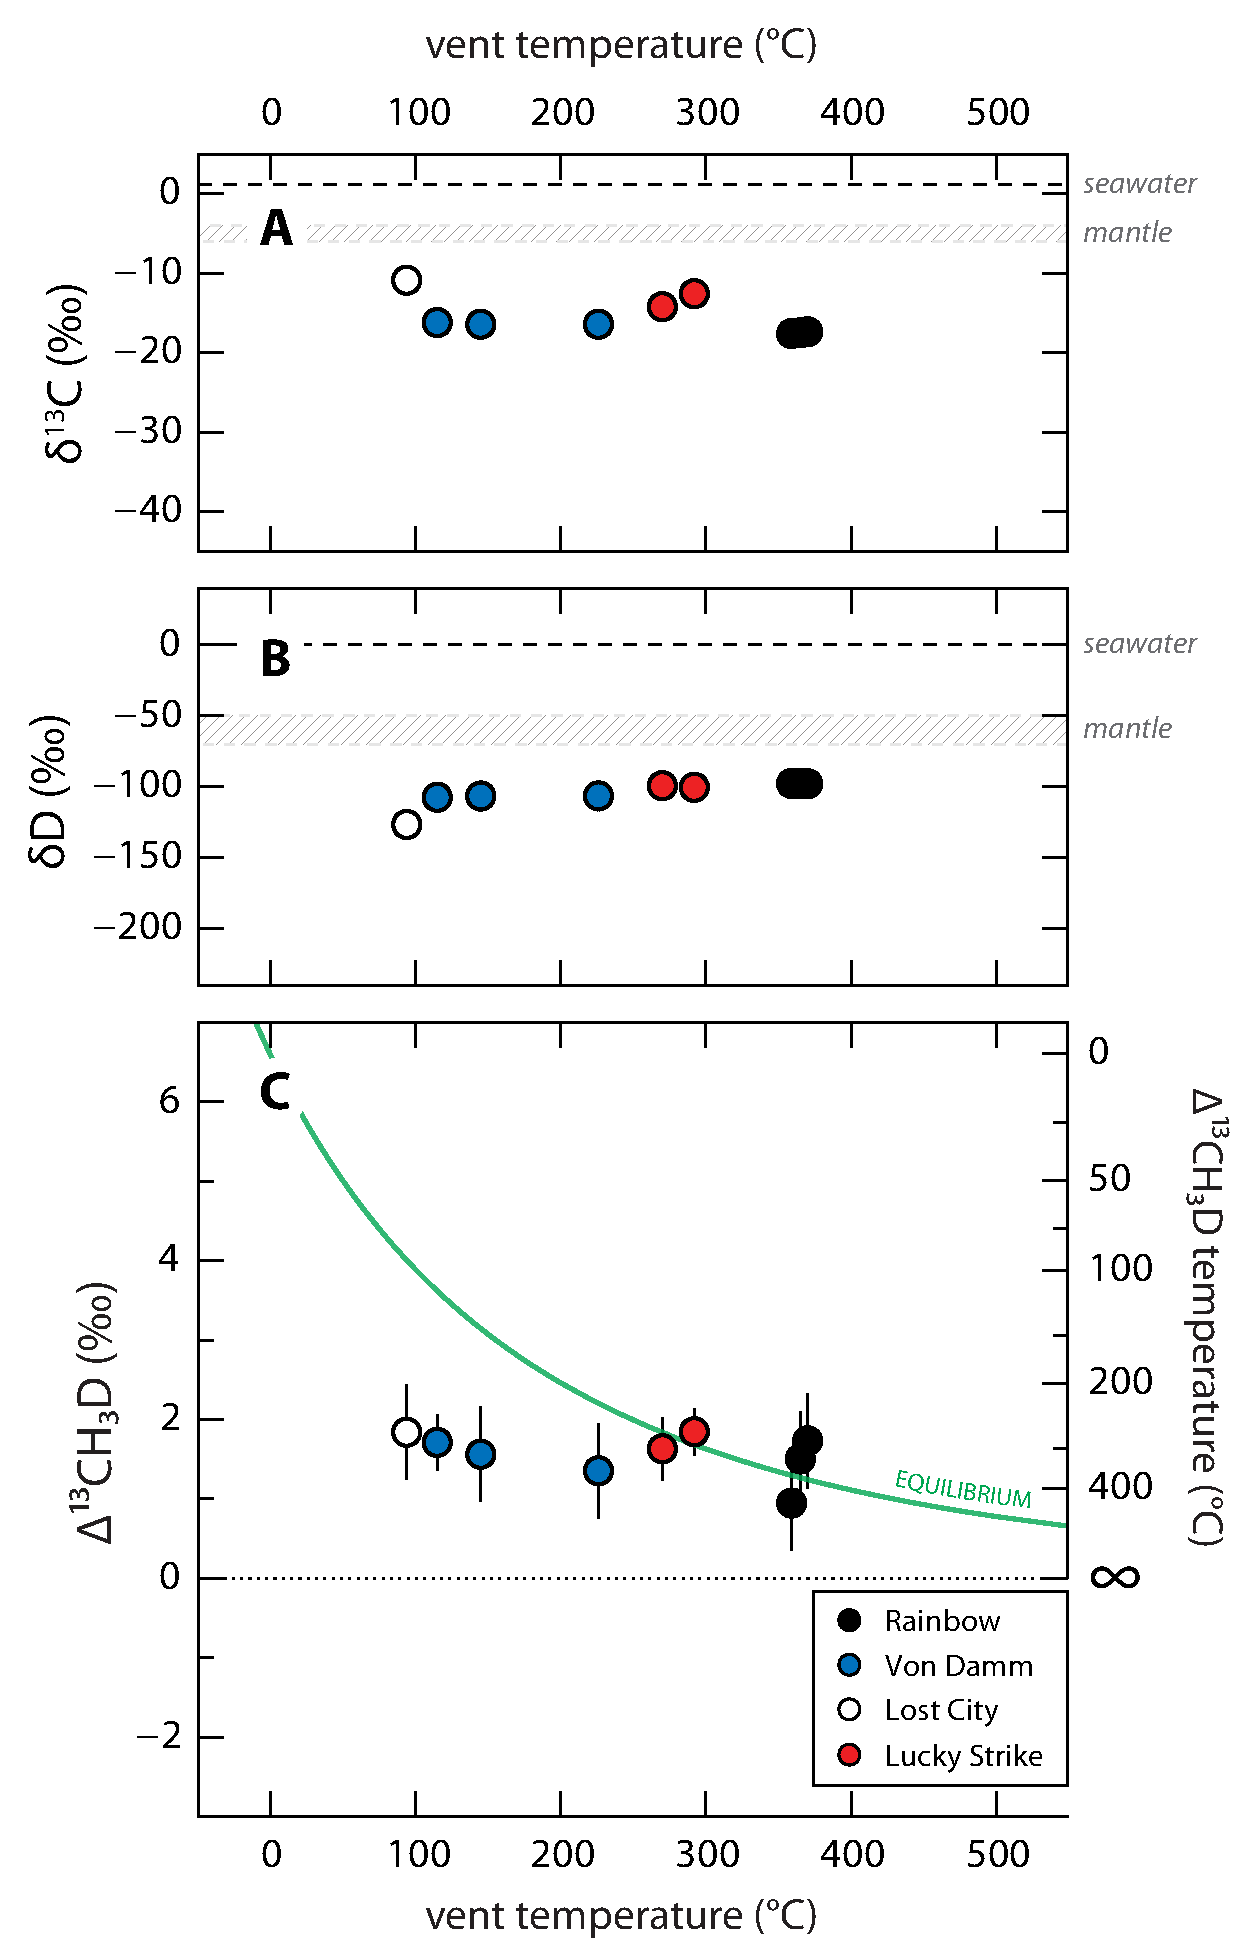
\includegraphics[width=0.6\linewidth]{figures/Fig3.1}
	\caption[Isotope and isotopologue ratios of methane at studied vent sites]{%
		Comparison of (\textbf{A}) δ\textsuperscript{13}C, (\textbf{B}) δD, and
		(\textbf{C}) Δ\textsuperscript{13}CH\textsubscript{3}D values of methane
		across vent sites. Data and error bars (95\% confidence interval) are
		from \autoref{tab:3:1}. In all panels, points are plotted against measured vent
		temperature (\autoref{tab:3:2}). The isotopic compositions of inorganic carbon (A)
		and hydrogen (B) in seawater and in the mantle are shown \parencite{Javoy++_1986_CG,Blank++_1993_GCA,Clog++_2013_EPSL}. In (C), the green line
		represents the clumped isotopologue composition at equilibrium. The
		Δ\textsuperscript{13}CH\textsubscript{3}D temperature scale corresponds
		to the calibration from \textcite{Wang++_2015_S}.
	}
	\label{fig:3:1}
\end{SCfigure*}


\begin{figure*}
	\centering
	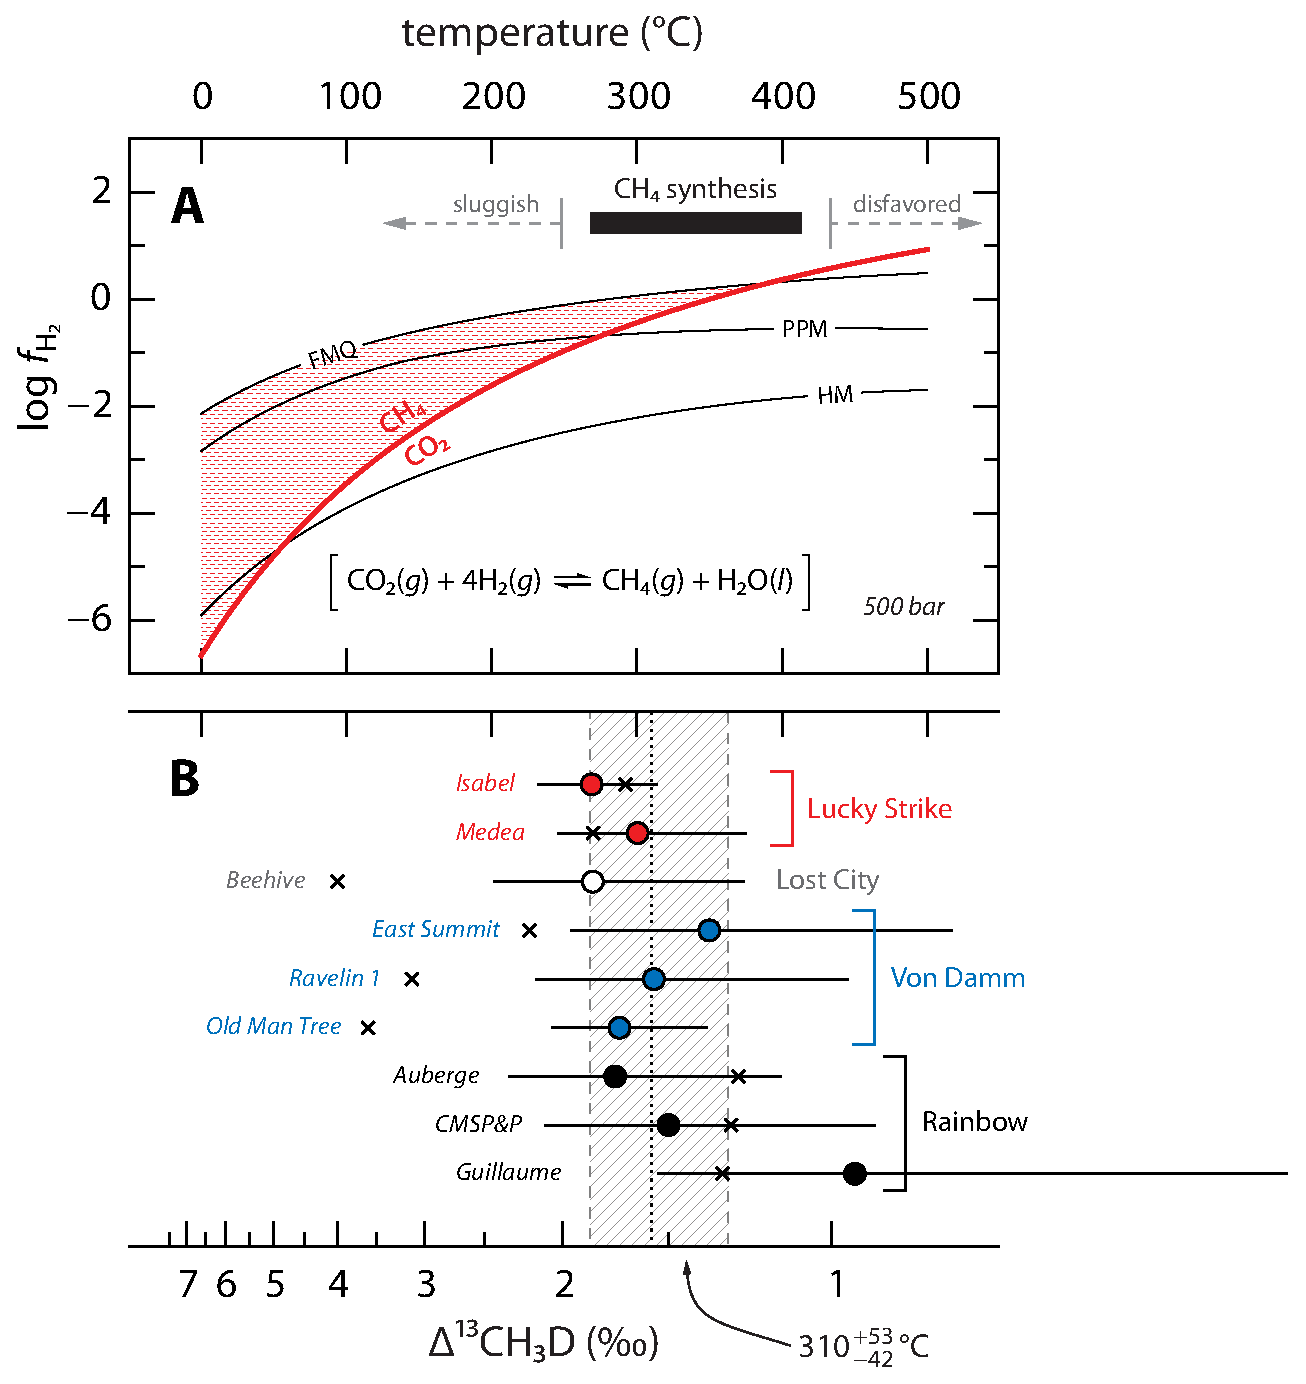
\includegraphics[width=0.75\linewidth]{figures/Fig3.2}
	\caption[Constraints on methane formation and stability from thermodynamics and
	clumped isotopologues]{%
		Constraints on methane formation and stability from thermodynamics and
		clumped isotopologue data. (\textbf{A}) Plot of fugacity of
		H\textsubscript{2} as a function of temperature at 500 bar, after \textcite{Shock_1992}. Red line represents the fugacity of H\textsubscript{2} at
		equilibrium, according to the reaction $ \ce{CO2\text{(\emph{g})}} + 4\ce{H2\text{(\emph{g})}} \leftrightharpoons
\ce{CH4\text{(\emph{g})}} + 2\ce{H2O\text{(\emph{l})}} $, when the fugacities of
		CH\textsubscript{4} and CO\textsubscript{2} are equal, and assuming unit
		activity for H\textsubscript{2}O(\emph{l}). Grey lines represent
		equilibrium H\textsubscript{2} fugacities buffered by the mineral
		assemblages fayalite-magnetite-quartz (FMQ), pyrite-pyrrhotite-magnetite
		(PPM), and hematite-magnetite (HM). Red shaded area represents the
		intersection of regions corresponding to geologically-relevant
		H\textsubscript{2} fugacity and where CH\textsubscript{4} is
		thermodynamically stable relative to CO\textsubscript{2}. The black bar
		represents the temperature range in which the evidence explored in this
		study suggests that methane synthesis is both favorable and facile on
		timescales of relevance to hydrothermal systems. (\textbf{B}) A
		``Caltech plot'' of the clumped isotopologue temperatures of methane
		from studied vents (data and error bars from \autoref{tab:3:1}). Equivalent
		Δ\textsuperscript{13}CH\textsubscript{3}D values are plotted on the
		bottom axis, and are derived from the calibration of \textcite{Wang++_2015_S}.
		The dotted line and gray hatching represent the mean ± 1\emph{s} of the
		Δ\textsuperscript{13}CH\textsubscript{3}D values across all studied
		vents (+1.57 ± 0.28‰, \emph{n} = 9). The × symbols mark measured vent
		temperatures (\autoref{tab:3:2}).
	}
	\label{fig:3:2}
\end{figure*}


Also shown in \autoref{tab:3:1} are results of methane clumped isotopologue
analyses. All samples yielded values of
Δ\textsuperscript{13}CH\textsubscript{3}D \textgreater{} 0‰, from which
apparent equilibrium temperatures can be derived (\mrefs[C]{Fig.}{fig:3:1} and \autoref{tab:3:1}).
The unweighted mean of the Δ\textsuperscript{13}CH\textsubscript{3}D
values across all nine vent fluids studied was 1.57 ± 0.28‰ (standard
deviation, 1\emph{s}), corresponding to a
Δ\textsuperscript{13}CH\textsubscript{3}D temperature of
\(310_{- 42}^{+ 53}\)~°C. Data for individual vent fluids were
analytically indistinguishable from this narrow range (\mrefs[B]{Fig.}{fig:3:2}).

\section{Discussion}\label{sec:3:discussion}

\subsection{\texorpdfstring{Decoupling of vent fluid chemistry and
		temperatures from conditions responsible for CH\textsubscript{4}
		synthesis}{Decoupling of vent fluid chemistry and temperatures from conditions responsible for CH4 synthesis}}\label{decoupling-of-vent-fluid-chemistry-and-temperatures-from-conditions-responsible-for-ch4-synthesis}

The four unsedimented submarine hydrothermal fields investigated in this
study include on- and off-axis vent fields at slow- to
ultraslow-spreading ridges, with host rock lithologies ranging from
mafic to ultramafic. Compositions of fluids from these sites partially
reflect this geological diversity. Supporting data for vent fluid
composition are shown in \autoref{tab:3:2}. Concentrations of CH\textsubscript{4}
in endmember fluids are high and lie within a range of 0.86 to 2.81 mM
(\mrefs[B]{Fig.}{fig:3:3}). Such high concentrations are typical of many
ultramafic-hosted mid-ocean ridge hydrothermal fields, whereas
basalt-hosted fields tend to have lower CH\textsubscript{4} contents \parencite[\textasciitilde{}0.1 mM;][]{McCollom+Seewald_2007_CR,Keir_2010_GRL}. In
this respect, concentrations of CH\textsubscript{4} in fluids at the
Lucky Strike field (\textasciitilde{}0.9 mM, \autoref{tab:3:2}), as well as at a
similar basalt-hosted field, Menez Gwen on the Mid-Atlantic Ridge \parencite[\textasciitilde{}1.7 mM,][]{Charlou++_2000_CG}, appear to be
anomalously elevated relative to those in other basalt-hosted settings
such as those on the fast-spreading East Pacific Rise, where
CH\textsubscript{4} concentrations of \textasciitilde{}0.1 mM are more
typical \parencite{McCollom+Seewald_2007_CR,Keir_2010_GRL}.


\begin{figure*}
	\centering
	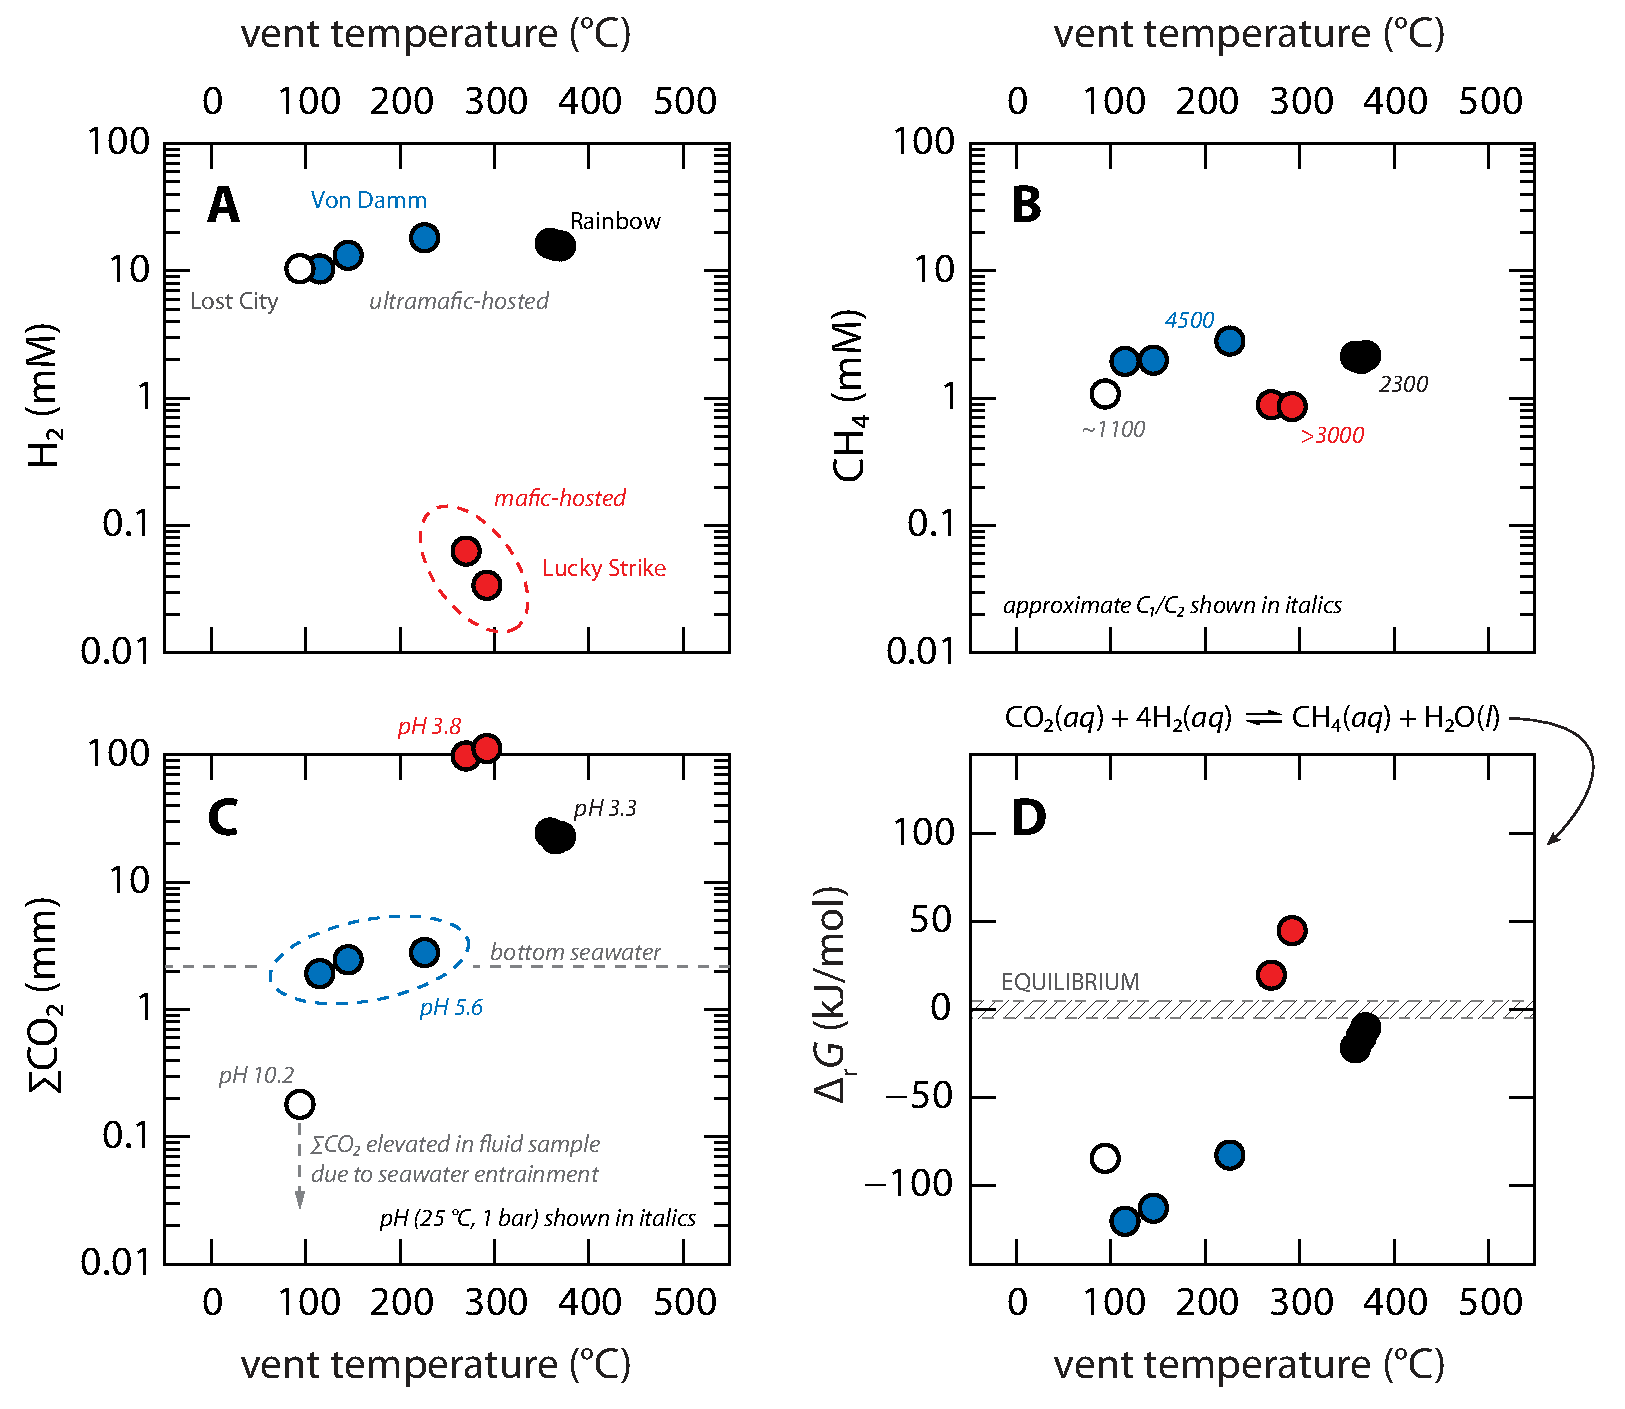
\includegraphics[width=0.95\linewidth]{figures/Fig3.3}
	\caption[Composition of vent fluids and energetics of methane synthesis in
		aqueous phase]{%
		Composition of vent fluids and energetics of methane synthesis in
		aqueous phase. Concentrations of (\textbf{A}) H\textsubscript{2},
		(\textbf{B}) CH\textsubscript{4}, and (\textbf{C}) $\big\sum\!$CO\textsubscript{2}
		are plotted against measured vent temperatures (data from \autoref{tab:3:2}). Also
		shown are molar ratios of methane to ethane
		(C\textsubscript{1}/C\textsubscript{2}, see \autoref{sec:3:results}) in (B), and pH
		values of endmember fluids in (C). (\textbf{D}) Gibbs energy of reaction
		for methane formation from CO\textsubscript{2} and H\textsubscript{2} in
		aqueous solution (\mrefs[]{Reaction}{eqn:3:2}), calculated at vent \emph{T} and \emph{P}
		conditions (Δ\textsubscript{r}\emph{G}, \autoref{tab:3:2}). Gray hatching
		represents thermodynamic equilibrium (taken as
		Δ\textsubscript{r}\emph{G} = 0 ± 5~kJ/mol). Methane formation in aqueous
		solution is thermodynamically favorable for points plotting below the
		hatched area. Symbol colors are the same as those in \mrefs[]{Figs.}{fig:3:1} and~\ref{fig:3:2}.
	}
	\label{fig:3:3}
\end{figure*}


Contents of low-molecular weight hydrocarbons are also similar between
the studied fields, with high C\textsubscript{1}/C\textsubscript{2}
ratios (\mrefs[B]{Fig.}{fig:3:3}) observed in fluids from Rainbow \parencite[\textasciitilde{}2300,][]{Charlou++_2002_CG}, Von Damm \parencite[\textasciitilde{}4500,][]{McDermott++_2015_PNAS}, Lost City \parencite[\textasciitilde{}1100,][]{Proskurowski++_2008_S}, and Lucky Strike \parencite[\textgreater{}3000,][]{Charlou++_2000_CG}. Such
high C\textsubscript{1}/C\textsubscript{2} ratios are typical of fluids
from unsedimented mid-ocean ridge hydrothermal systems \parencite{McCollom+Seewald_2007_CR}.

Except for the Lost City fluids, total dissolved inorganic carbon
($\big\sum\!$CO\textsubscript{2} = CO\textsubscript{2}(\emph{aq}) +
\(\mathrm{\text{HC}}\mathrm{O}_{\mathrm{3}}^{\mathrm{-}}\) +
\(\mathrm{C}\mathrm{O}_{\mathrm{3}}^{\mathrm{2 -}}\)) concentrations are comparable to or 
higher than CH\textsubscript{4} and are characterized by a wider range
of values (1.9 to 112.0 mmol/kg, \mrefs[C]{Fig.}{fig:3:3}). Endmember fluids from
Rainbow, Von Damm, and Lucky Strike contain 2 to 50 times as much total
carbon as is in bottom seawater \parencite[\textasciitilde{}2.2 mM;][]{McDermott++_2015_PNAS,Reeves++_2014_PNAS}, such that $\big\sum\!$CO\textsubscript{2} in
recharging seawater cannot be the sole source of carbon to venting
fluids. The Lost City fluid contains very low amounts of
$\big\sum\!$CO\textsubscript{2} (\textasciitilde{}0.18~mmol/kg), the majority of
which is likely derived from seawater entrainment during sample
collection \parencite{Reeves++_2014_PNAS}. Given the high pH (10.2), the
concentration of CO\textsubscript{2}(\emph{aq}) in endmember Lost City
fluids must be very low (see footnote~g in \autoref{tab:3:2}). At the relatively low
pH of the other fluids (3.33 to 5.81), the majority of $\big\sum\!$CO\textsubscript{2} is in the form of CO\textsubscript{2}(\emph{aq}).
%\begin{center}
\begin{table}[t]
	
	\centering
	
	\caption[Fluid compositions and Gibbs energy of reaction (Δ\textsubscript{r}\emph{G}) for
		abiotic methane formation at studied vent
		sites]{Fluid compositions\textsuperscript{a} used in thermodynamic calculations
		and calculated Gibbs energy of reaction (Δ\textsubscript{r}\emph{G}) for
		abiotic methane formation via \mrefs{Reaction}{eqn:3:2} at studied vent
		sites.\textsuperscript{b}}
	\label{tab:3:2}
	
	\begin{threeparttable}
		\small
		%\hspace*{-1ex}
		\begin{tabular}[]{@{} l l @{\!} r r r d{4} d{4} d{4} d{4} @{\!\!\!}}
			\toprule
%			{Field} & Vent & \emph{T} (°C)\textsuperscript{c} & \emph{P} (bar) & pH\textsuperscript{d} & $\big\sum\!$CO\textsubscript{2} (mm) & H\textsubscript{2} (mM) & CH\textsubscript{4} (mM) & Δ\textsubscript{r}\emph{G} (kJ/mol)\textsuperscript{e}\tabularnewline
			{Field} & Vent & \emph{T} (°C)\textsuperscript{c} & \emph{P} (bar) & pH\textsuperscript{d} & \multicolumn{1}{c}{$\big\sum\!$\ce{CO2} (mm)} & \multicolumn{1}{c}{\ce{H2} (mM)} & \multicolumn{1}{c}{\ce{CH4} (mM)} & \multicolumn{1}{c}{$\Delta_\text{r}G$ (kJ/mol)\textsuperscript{e}}\tabularnewline
			\midrule
			{Rainbow} & Guillaume & 361 & 230 & 3.33 & 24.3 & 16.5 & 2.13 & 
			-22\tabularnewline
			& CMSP\&P & 365 & 230 & 3.36 & 21.9 & 15.9 & 2.05 & -16\tabularnewline
			& Auberge & 370 & 230 & 3.35 & 22.8 & 15.7 & 2.16 & -11\tabularnewline
			{Von Damm} & Old Man Tree\textsuperscript{f} & 115 & 235 & 5.81 &
			1.80 & 10.5 & 1.97 & -121\tabularnewline
			& Ravelin 1\textsuperscript{f} & 145 & 235 & 5.83 & 2.52 & 13.4 & 2.02 &
			-113\tabularnewline
			& East Summit & 226 & 235 & 5.56 & 2.80 & 18.2 & 2.81 &
			-83\tabularnewline
			{Lost City} & Beehive & 96 & 70 & 10.20 & 0.18\textsuperscript{g}
			& 10.4 & 1.08 & -85\tabularnewline
			{Lucky Strike} & Medea & 270 & 170 & 3.81 & 98.0 & 0.063 & 0.89 &
			+20\tabularnewline
			& Isabel & 292 & 170 & 3.81 & 112.0 & 0.034 & 0.86 & +45\tabularnewline
			\bottomrule
		\end{tabular}
		%\hspace*{-1ex}	
		\begin{tablenotes}
			\item Analytical uncertainties (2\emph{s}) are ±2~°C for \emph{T}; ±5\% for
			H\textsubscript{2}, $\big\sum\!$CO\textsubscript{2}, and CH\textsubscript{4}; and
			±0.05 units for pH. Abbreviations: mm, mmol/kg fluid; mM, mmol/L fluid.
			
			\item \textsuperscript{a} All concentrations shown are extrapolated to
			endmember fluid composition (regressed to zero Mg content), except where
			noted. Data are from \textcite{McDermott++_2015_PNAS,Reeves++_2014_PNAS}.
			
			\item \textsuperscript{b} For each vent fluid, the energetic favorability of
			methane formation via this reaction was assessed by calculating the
			Gibbs energy of reaction (Δ\textsubscript{r}\emph{G}), defined by the
			relationship: Δ\textsubscript{r}\emph{G} = \emph{RT}
			ln(\emph{Q}/\emph{K}), where \emph{R} is the universal gas constant,
			\emph{T} is measured fluid temperature in kelvin, \emph{Q} is the
			reaction quotient, and \emph{K} is the equilibrium constant at \emph{T}
			and seafloor pressure \emph{P}. Equilibrium constants were calculated
			using thermodynamic data and standard states from \textcite{Johnson++_1992_CnG,Shock+Helgeson_1990_GCA}. For all calculations, the activity of
			H\textsubscript{2}O(\emph{l}) was assumed to be unity. Activity
			coefficients were assumed to be unity for neutral dissolved species. For
			all fluids except for that from Lost City,\textsuperscript{g} the
			concentration of CO\textsubscript{2}(\emph{aq}) was assumed to be equal
			to $\big\sum\!$CO\textsubscript{2}, a reasonable approximation given the low
			measured shipboard pH values and calculated equilibrium speciation of
			dissolved carbonate species at \emph{in situ} temperatures and seafloor
			pressures.
			
			\item \textsuperscript{c} Maximum measured vent temperature.
			
			\item \textsuperscript{d} Shipboard pH measurement (25~°C and 1 atm).
			
			\item \textsuperscript{e} A negative value of Δ\textsubscript{r}\emph{G}
			indicates a thermodynamic drive for the reaction to proceed as written
			from left to right (i.e., methane formation favored). Given
			uncertainties associated with chemical analyses and thermodynamic data,
			calculated Δ\textsubscript{r}\emph{G} values within ±5 kJ/mol of zero
			are interpreted to indicate that the reaction has approached or attained
			a state of thermodynamic equilibrium \parencite{Seewald_2001_GCA_minerals}.
			
			\item \textsuperscript{f} Concentrations for fluids from Old Man Tree and
			Ravelin 1 at Von Damm not extrapolated to zero Mg; Mg contents for these
			fluids are 14.0 and 15.0 mmol/kg fluid, respectively, indicating that
			endmember fluid has already mixed with seawater in the subsurface prior
			to discharge at the seafloor \parencite{McDermott++_2015_PNAS}.
			
			\item \textsuperscript{g} An arbitrary CO\textsubscript{2}(\emph{aq})
			concentration of 1 nmol/kg was used in thermodynamic calculations for
			the Lost City fluid, similar to \textcite{Reeves++_2014_PNAS}. The actual
			concentration value is subject to substantial uncertainty due to
			difficulties in determining the near-zero endmember $\big\sum\!$CO\textsubscript{2}
			content in vent fluids, given that some entrainment of
			$\big\sum\!$CO\textsubscript{2}-replete seawater always occurs during sampling
			\parencite{Proskurowski++_2008_S}. Varying this value by as much as ten orders
			of magnitude would not affect the conclusion that methane formation is
			thermodynamically favorable in the fluid, due to the high
			H\textsubscript{2} content and the power of 4 to which the activity of
			H\textsubscript{2}(\emph{aq}) is raised in the mass action expression.
	

		\end{tablenotes}

	\end{threeparttable}

\end{table}
%\end{center}

The concentration of dissolved H\textsubscript{2} is high and varies
from 10.4 to 18.2 mM in endmember and mixed fluids from the Rainbow, Von
Damm, and Lost City fields, whereas fluids from Lucky Strike have
approximately three orders of magnitude lower concentrations (34--63~µM,
\mrefs[A]{Fig.}{fig:3:3}). At Rainbow, Von Damm, and Lost City, serpentinization of
ultramafic rock in subsurface reaction zones with concomitant production
of H\textsubscript{2} is thought to be a major control on fluid
compositions \parencite{Kelley++_2001_N,Charlou++_2002_CG,McDermott++_2015_PNAS}. In contrast, the Lucky Strike field is hosted in basaltic
rock, and vent fluids there encounter much more oxidizing conditions \parencite{Charlou++_2000_CG,Pester++_2012_GCA}.

The stoichiometry of the reaction
\begin{equation}\label{eqn:3:2}
\ce{CO2\text{(\emph{aq})}} + 4\ce{H2\text{(\emph{aq})}} \leftrightharpoons
\ce{CH4\text{(\emph{aq})}} + 2\ce{H2O\text{(\emph{l})}}
\end{equation}
indicates that the abundance of CH\textsubscript{4}(\emph{aq}) at
thermodynamic equilibrium in vent fluids should be highly sensitive to
the concentration of H\textsubscript{2} because of the fourth-power
dependence on the activity of H\textsubscript{2}(\emph{aq}) in the
corresponding mass action expression. At Lucky Strike, formation of
CH\textsubscript{4}(\emph{aq}) in endmember fluids is thermodynamically
disfavored due to the low H\textsubscript{2} contents (\autoref{tab:3:2}). In all
other vent fluids studied, a thermodynamic drive for methane synthesis
is present at varying magnitudes (\mrefs[D]{Fig.}{fig:3:3}).

Methane \textsuperscript{13}C/\textsuperscript{12}C and D/H ratios are
similar across fluids from all four unsedimented hydrothermal fields
studied (\autoref{fig:3:1}). The δ\textsuperscript{13}C values ($-$18‰ to $-$11‰) are
within the range of those determined for methane at more than a dozen
other basalt- and ultramafic-hosted submarine hydrothermal systems
studied to date ($-$24‰ to $-$6‰), including Kairei on the Central Indian
Ridge, TAG, Broken Spur, and Logatchev on the Mid-Atlantic Ridge, and
17--19°S, 9°50$'$N, 13°N, and 21°N on the East Pacific Rise \parencite[see][and references therein]{Keir_2010_GRL,McCollom+Seewald_2007_CR}. Published
data for δD of methane are more limited; however, the δD values we
measured ($-$127‰ to $-$98‰) are similar to those determined at Logatchev \parencite[$-$109‰][]{Proskurowski++_2006_CG}  and 21°N on the East Pacific Rise \parencite[$-$126‰ to $-$102‰][]{Welhan+Craig_1983}.
\renewcommand{\textfraction}{0.1}  	% How much text there must be at bottom of float https://tex.stackexchange.com/a/39020
\renewcommand{\floatpagefraction}{0.9}	% only pages with more than 80% of floats, will become pure float-only pages. The default is 0.6

The data described above support the general consensus that the methane
in the studied hydrothermal fluids is of dominantly abiotic origin \parencite[e.g.,][]{Charlou++_2002_CG,McDermott++_2015_PNAS,Proskurowski++_2008_S,Welhan_1988_CG}, and that contributions of thermogenic or
microbial sources of methane are limited or insignificant. Because the
four sites studied lack substantial sediment burdens, organic carbon
from which thermogenic hydrocarbons or microbial methane can be
generated is in scarce supply \parencite{Welhan_1988_CG,Reeves++_2014_PNAS}.
Furthermore, high C\textsubscript{1}/C\textsubscript{2} ratios
(\textasciitilde{}1000 to 4000), along with high methane
δ\textsuperscript{13}C values ($-$18‰ to $-$11‰), are distinct from
thermogenic or microbial sources, which typically have lower
C\textsubscript{1}/C\textsubscript{2} ratios or lower
δ\textsuperscript{13}C values, respectively \parencite{McCollom+Seewald_2007_CR}.

The methane δ\textsuperscript{13}C data alone do not unambiguously
exclude contributions of microbial methanogenesis, because high methane
δ\textsuperscript{13}C values could be a result of near-quantitative
conversion of $\big\sum\!$CO\textsubscript{2} to CH\textsubscript{4}, particularly
under $\big\sum\!$CO\textsubscript{2}-limited and/or high-pressure conditions such as those present at
Lost City \parencite{Brazelton++_2006_AEM,Bradley+Summons_2010_EPSL,Takai++_2008_PNAS}. However,
radiocarbon (\textsuperscript{14}C) abundances for methane from Lost
City and Von Damm are very low {[}fraction modern
(\emph{F}\textsubscript{m}) averaging 0.004--0.006, near the limit of
detection (\emph{F}\textsubscript{m} \textasciitilde{} 0.003){]}
\parencite{Proskurowski++_2008_S,McDermott++_2015_PNAS}, whereas
\textsuperscript{14}C contents of endmember $\big\sum\!$CO\textsubscript{2} at Von
Damm are \textasciitilde{}5× higher \parencite{McDermott++_2015_PNAS}. Had
CH\textsubscript{4} been derived from reduction of $\big\sum\!$CO\textsubscript{2},
the younger \textsuperscript{14}C age of the $\big\sum\!$CO\textsubscript{2} would
have been transferred to CH\textsubscript{4}. \textcite{McDermott++_2015_PNAS}
further showed that $\big\sum\!$CO\textsubscript{2} in the vent fluids at Von Damm
is likely seawater-derived, because both concentrations and
δ\textsuperscript{13}C values of endmember $\big\sum\!$CO\textsubscript{2} match
those of local bottom seawater. The apparent conservation of
$\big\sum\!$CO\textsubscript{2} during convective circulation at Von Damm indicates
that $\big\sum\!$CO\textsubscript{2} in recharging seawater at Von Damm has not
been converted to CH\textsubscript{4} via any process---microbial or
otherwise---despite high energetic favorability for CH­\textsubscript{4}
synthesis (\mrefs[D]{Fig.}{fig:3:3}). Similar carbon isotopic compositions of
CH\textsubscript{4} and contents of C\textsubscript{2+} alkanes at Lost
City, Lucky Strike, and Rainbow (as well as at other unsedimented fields
studied to date), despite marked differences in geologic setting, fluid
composition, and thermodynamic drive for CH\textsubscript{4} synthesis,
are consistent with a common abiotic origin for methane at many, if not
all, sediment-poor seafloor hydrothermal systems.
\begin{SCfigure*}
	\centering
	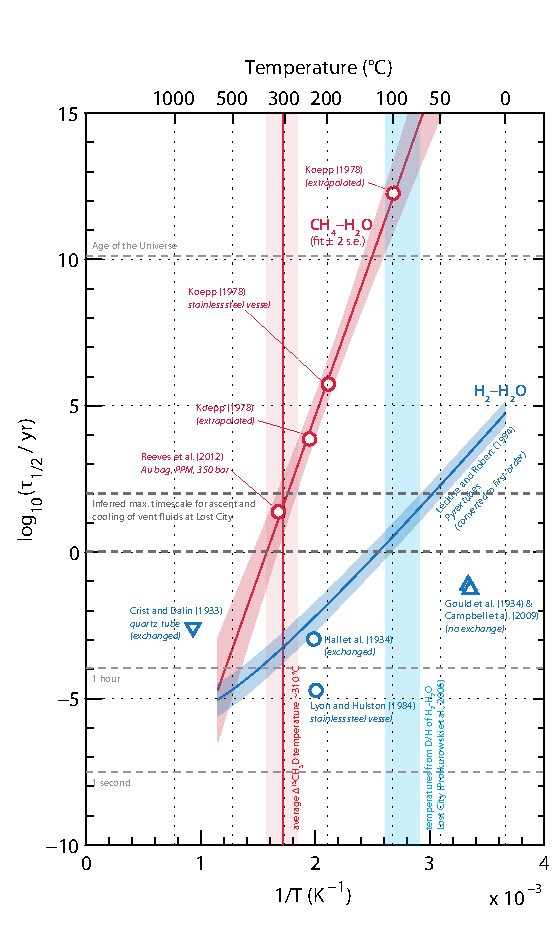
\includegraphics[width=0.625\linewidth]{figures/Fig3.4}
	\caption[Half-exchange timescales for hydrogen exchange between CH\textsubscript{4} \& H\textsubscript{2}O
 and H\textsubscript{2} \& H\textsubscript{2}O ]{%
		Half-exchange time\-scales ($\tau_{1/2} = \ln(2)/k$) for
		hydro\-gen exchange between CH\textsubscript{4} \& H\textsubscript{2}O
		(red sym\-bols) and H\textsubscript{2} \& H\textsubscript{2}O (blue) based
		on experiments done in the absence of added catalyst
		\parencite{Crist+Dalin_1933_JCP,Hall++_1934_JACS,Gould++_1934_JCP,Koepp_1978,Lyon+Hulston_1984_GCA,Lecluse+Robert_1994_GCA,Campbell++_2009_GCA,Reeves++_2012_GCA}.
	 	Reactions were assumed to be first order in
		CH\textsubscript{4} or H\textsubscript{2}. When rate constants were not
		provided by the authors or when exchange was not observed, the reported
		duration of the experiment was taken as an estimate of the timescale of
		exchange. Downward- and upward-pointing triangles are, respectively,
		maximum and minimum estimates of the exchange timescale. The
		$\tau_{1/2}$ for CH\textsubscript{4}--H\textsubscript{2}O
		exchange from \textcite{Reeves++_2012_GCA} comes from \autoref{fig:3:S2}.
		Second-order rate coefficients for
		H\textsubscript{2}--H\textsubscript{2}O exchange from \textcite{Lecluse+Robert_1994_GCA} were converted to first-order rate coefficients by multiplying by
		the equilibrium vapor pressure of H\textsubscript{2}O calculated at
		temperatures \emph{T} and a pressure of 1~kbar. Uncertainties in
		exchange rates are difficult to estimate, but are probably one order of
		magnitude or greater. Clumped isotopologue temperatures for
		CH\textsubscript{4} from the present study (red bar) and temperatures
		from D/H geothermometry of H\textsubscript{2}--H\textsubscript{2}O in
		endmember fluids at the Lost City site (blue bar) \parencite{Proskurowski++_2006_CG} are also shown. See text for interpretation of these data with
		respect to timescales of fluid circulation.
	}
	\label{fig:3:4}
\end{SCfigure*}

Measured Δ\textsuperscript{13}CH\textsubscript{3}D values (averaging
1.57 ± 0.28‰, 1\emph{s}) and corresponding apparent equilibrium
temperatures (\(310_{- 42}^{+ 53}\)~°C) are strikingly uniform in the
context of the large natural variations (up to ca.\ 10‰) previously
observed in Δ\textsuperscript{13}CH\textsubscript{3}D values carried by
methane sampled from different settings \parencite{Wang++_2015_S}.
Furthermore, the studied fluids vented at a wide range of temperatures,
ranging from 96 to 370~°C. Had the methane in these samples attained
isotopologue equilibrium at measured vent temperatures,
Δ\textsuperscript{13}CH\textsubscript{3}D values from 4.0 to 1.3‰,
respectively, would be expected. The observed range of clumped
isotopologue data is much smaller than this predicted range (\mrefs[C]{Fig.}{fig:3:1}),
with Δ\textsuperscript{13}CH\textsubscript{3}D temperatures generally
equal to or higher than fluid temperatures (\mrefs[B]{Fig.}{fig:3:2}). In
lower-temperature (\textless{}250~°C) fluids, including fluids that have
mixed in the subsurface (venting with non-zero Mg) such as those from
Ravelin 1 (145~°C) and Old Man Tree (115~°C) vents at Von Damm
\parencite{McDermott++_2015_PNAS}, Δ\textsuperscript{13}CH\textsubscript{3}D
temperatures higher than fluid temperatures indicate that
Δ\textsuperscript{13}CH\textsubscript{3}D values have not been affected
by cooling below \textasciitilde{}250~°C. In higher temperature fluids
(\textgreater{}270~°C) however,
Δ\textsuperscript{13}CH\textsubscript{3}D temperatures are analytically
indistinguishable from measured fluid temperatures. Experimental data
suggest that hydrogen exchange between methane and water in hydrothermal
fluids may be observable at temperatures of \textasciitilde{}325~°C on
relatively short timescales \parencite[years;][and \autoref{fig:3:S2}]{Reeves++_2012_GCA}
relevant to hydrothermal systems (\autoref{fig:3:4}). Hydrogen exchange between
CH\textsubscript{4} and H\textsubscript{2}O may explain the uniformity
of both δD and Δ\textsuperscript{13}CH\textsubscript{3}D values of
methane in high-temperature fluids (\autoref{fig:3:5}); the implications of this
are discussed below (\autoref{hydrogen-exchange-and-the-origin-of-hydrogen-in-ch4}). The
Δ\textsuperscript{13}CH\textsubscript{3}D values indicate that
CH\textsubscript{4} experienced temperatures of at least 300~°C during
its residence within the oceanic crust. Our methane clumped isotopologue
data indicate that temperatures and compositions of hot-spring fluids at
the time of venting are decoupled from the conditions responsible for
the formation of CH\textsubscript{4} in these fluids. The following
sections discuss how the 300~°C or greater inferred temperatures are
compatible with models invoking respeciation of magmatic volatiles at
those temperatures to form CH\textsubscript{4} in plutonic layers of the
oceanic crust.

\subsection{\texorpdfstring{Hydrogen exchange and the origin of
		hydrogen in
		CH\textsubscript{4}}{Hydrogen exchange and the origin of hydrogen in CH4}}\label{hydrogen-exchange-and-the-origin-of-hydrogen-in-ch4}

Hydrogen isotope ratio measurements provide constraints on the origin of
the major H-bearing species within vent fluids. Apparent temperatures
derived from D/H equilibria in the systems
H\textsubscript{2}--H\textsubscript{2}O and
H\textsubscript{2}--CH\textsubscript{4} were first used as
geothermometers in studies of geothermal or volcanic gases and waters
\parencite{Arnason_1977_Geothermics,Arnason+Sigurgeirsson_1968_GCA,Gunter+Musgrave_1971_GCA,Panichi++_1977_Geothermics,Panichi+Gonfiantini_1977_Geothermics,Kiyosu_1983_EPSL,Lyon+Hulston_1984_GCA}, and later examined with respect to data from
seafloor hydrothermal fluids \parencite{Welhan+Craig_1983,Horibe+Craig_1995_GCA,Proskurowski++_2006_CG,Bradley+Summons_2010_EPSL,Kawagucci++_2010_JGR,Kawagucci++_2011_GcJ,Kawagucci++_2013_CG}, shield-hosted groundwaters
\parencite{SherwoodLollar++_1993_GCA_abiogenic,SherwoodLollar++_2007_Ab,SherwoodLollar++_2008_GCA}, and continental
springs, seeps, and well fluids influenced by serpentinization \parencite{Fritz++_1992,Neal+Stanger_1983_EPSL,Coveney++_1987_AAPGB,Abrajano++_1988_CG,Etiope++_2011_CG,Suda++_2014_EPSL}. Temperatures returned from
H\textsubscript{2}--H\textsubscript{2}O and
H\textsubscript{2}--CH\textsubscript{4} equilibria often agree with each
other and with realistic geologic and hydrologic scenarios for
geothermal fluids exiting at high temperatures, but these relationships
do not necessarily hold for lower-temperature fluids. 

\textcite{Proskurowski++_2006_CG} showed that D/H-based temperatures derived
from H\textsubscript{2}--H\textsubscript{2}O and
H\textsubscript{2}--CH\textsubscript{4} in high-temperature vent fluids
(\textgreater{}270~°C) are concordant and match measured fluid
temperatures at discharge. At the low-temperature Lost City site,
however, H\textsubscript{2}--H\textsubscript{2}O and  
H\textsubscript{2}--CH\textsubscript{4} yielded discordant temperatures
of 70--110~°C and 110--150~°C, respectively. \textcite{Proskurowski++_2006_CG}
reconciled these data by suggesting that serpentinization of ultramafic
basement rocks beneath the Lost City vent field occurs at low
temperatures of 110--150~°C, concomitant with production of both
H\textsubscript{2} and CH\textsubscript{4}, and that H\textsubscript{2}
maintained isotopic equilibrium with H\textsubscript{2}O during slow
cooling of root-zone fluids to ca.\ 70--110~°C prior to rapid ascent to
seafloor while the higher temperature signal recorded by
H\textsubscript{2}--CH\textsubscript{4} was presumably not reset during
cooling. In contrast, the Δ\textsuperscript{13}CH\textsubscript{3}D
temperature of \(270_{- 68}^{+ 104}\)~°C we obtained for the Beehive
vent fluid argues for a much higher temperature of last exchange for the
C--H bonds in methane, and does not support suggestions of
CH\textsubscript{4} production at lower temperatures. The clumped
isotopologue temperature is consistent with estimates from heat balance
considerations, δ\textsuperscript{18}O values, and alkane-alkene and
mineral-fluid equilibria all suggesting that Lost City fluids
experienced temperatures as high as 250~°C at depth \parencite{Allen+Seyfried_2004_GCA,Foustoukos++_2008_GCA,Reeves++_2012_GCA,Seyfried++_2015_GCA}. Discrepancies between measured
Δ\textsuperscript{13}CH\textsubscript{3}D temperatures, temperatures
from D/H geothermometry, and fluid exit temperatures at Lost City
indicate that rather than directly recording the temperatures of
H\textsubscript{2} and CH\textsubscript{4} synthesis, each
geothermometer records a different portion of the time-temperature
history of the fluids.

\afterpage{%
	\clearpage
	
	\begin{landscape}
	
		\begin{figure*}[p]
			\centering
			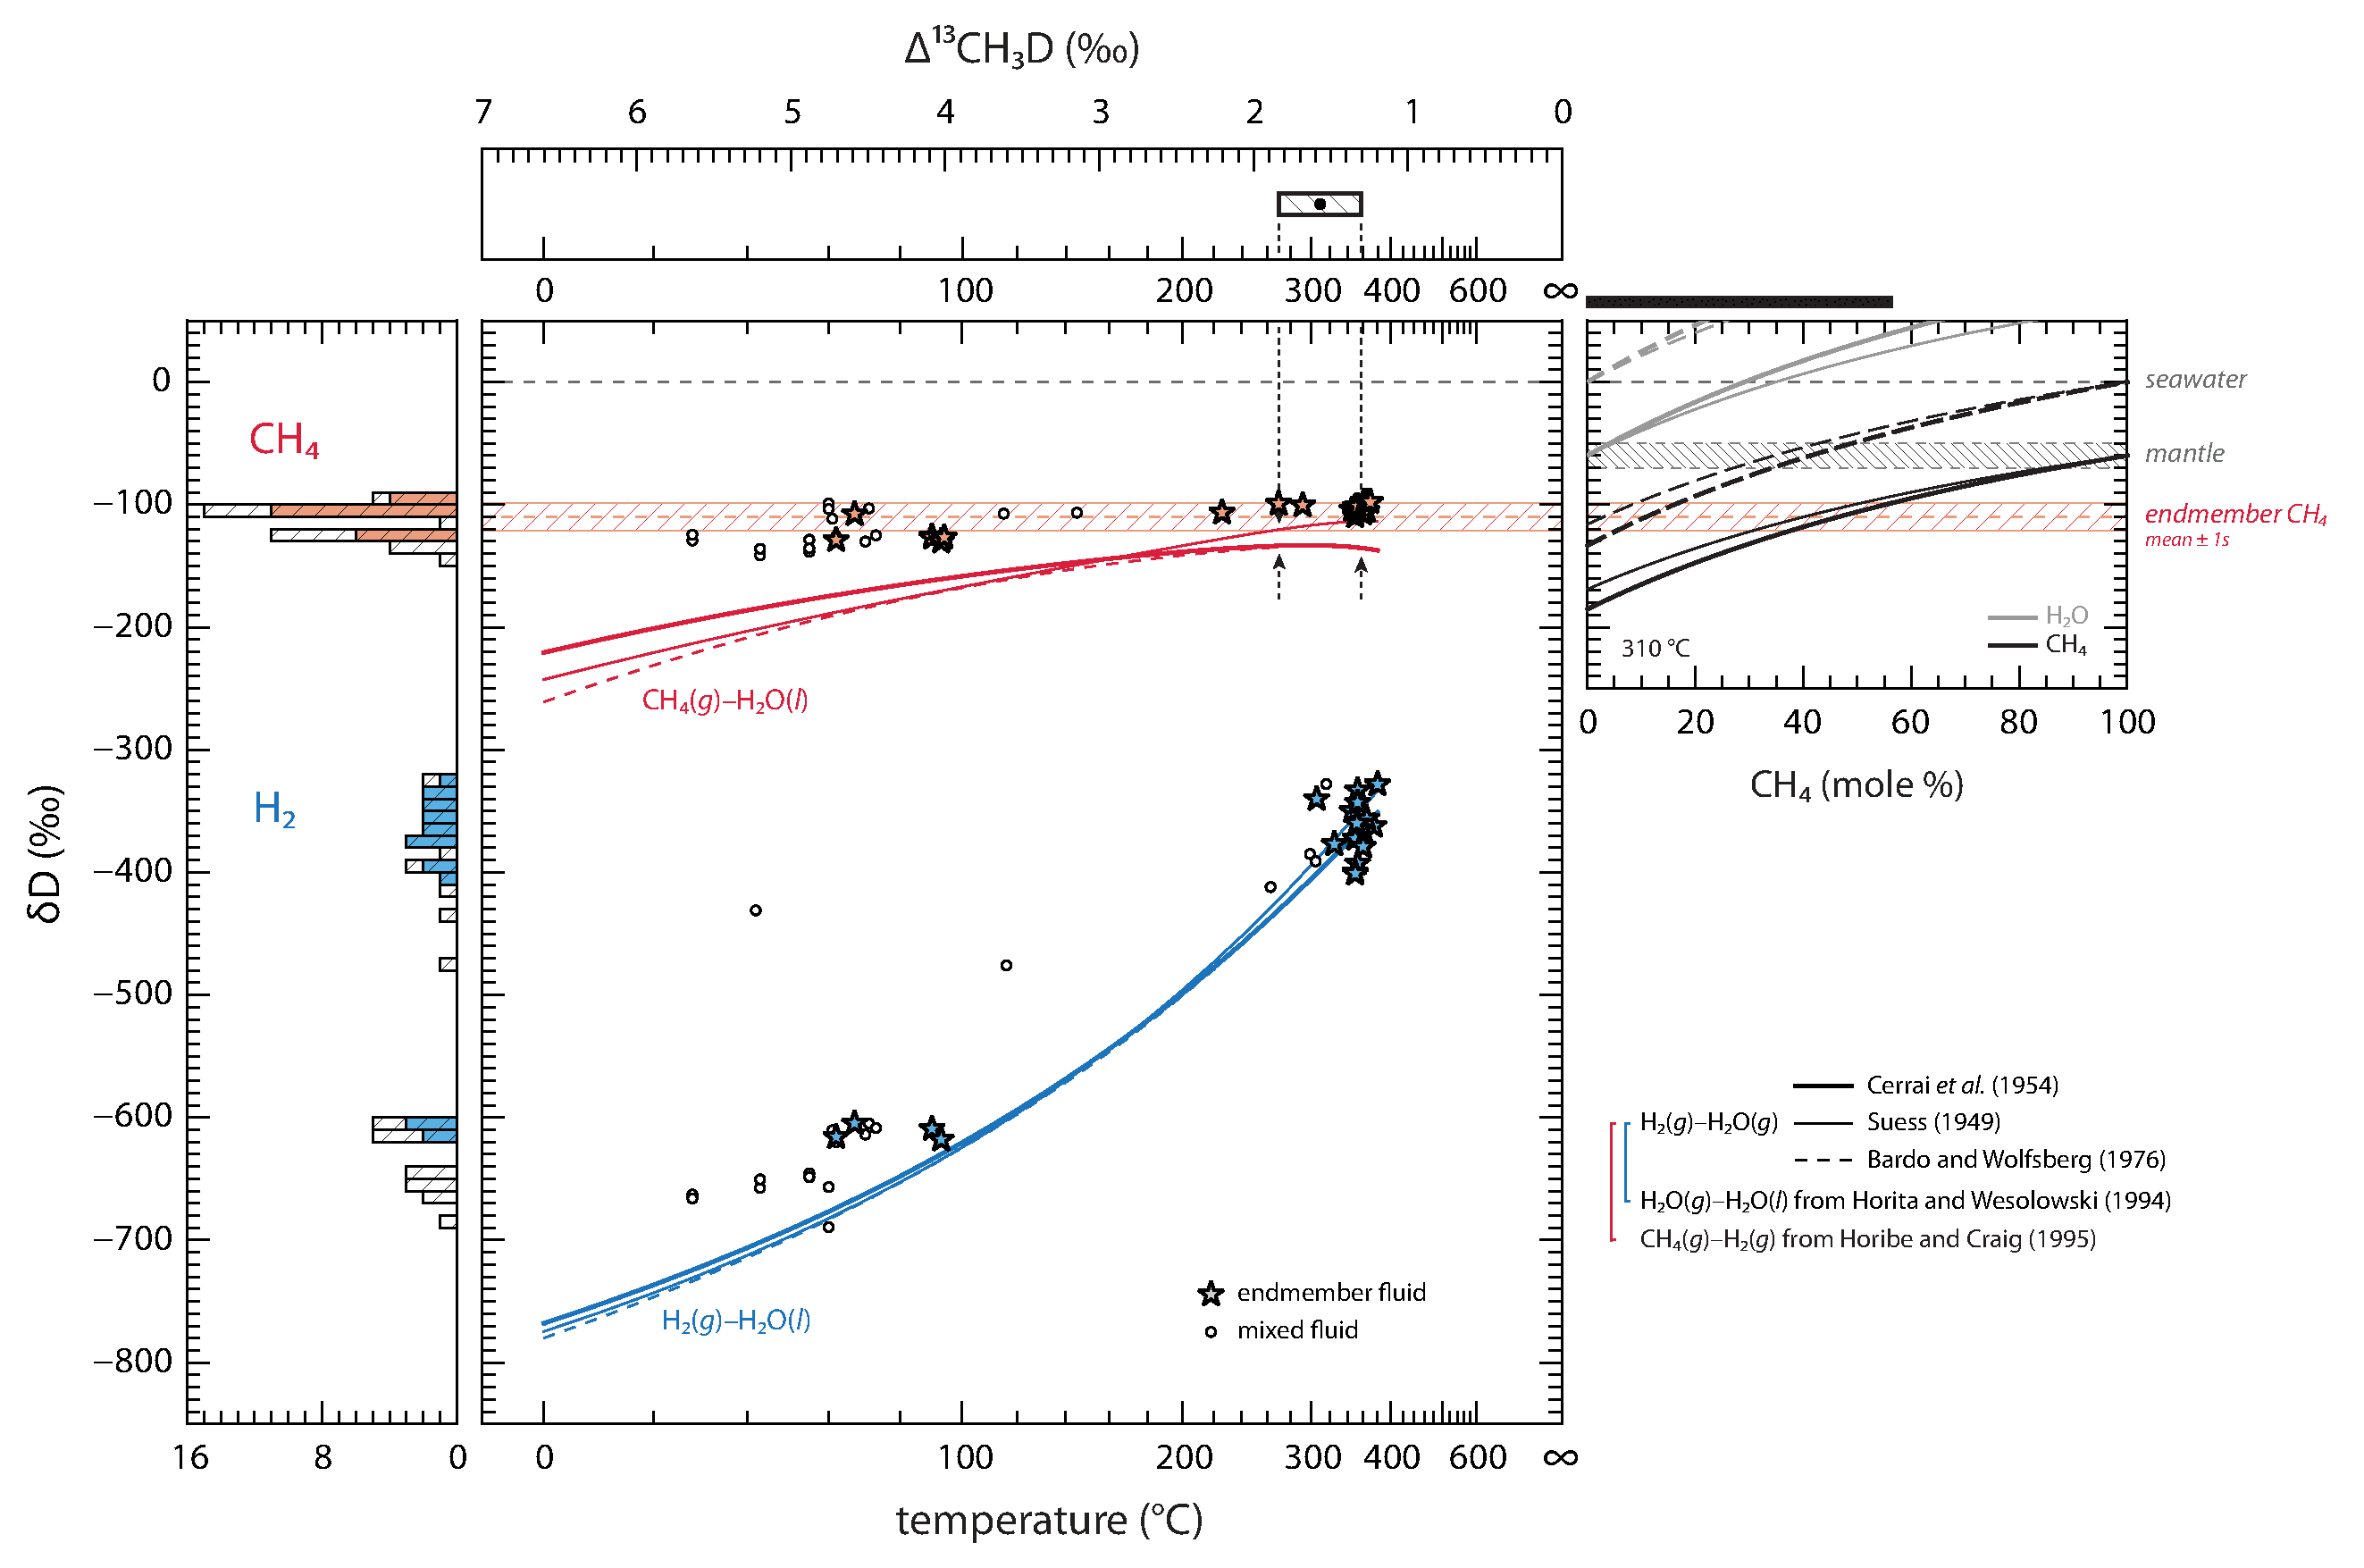
\includegraphics[width=\linewidth]{figures/Fig3.5}
			
			
			
		\end{figure*}
	
	\end{landscape}
	%\addtocounter{figure*}{-1}	% decrement counter because putting figure caption in next float
	
	\begin{landscape}
		
		\begin{figure*}[h!]
			\caption[Data and models of D/H of CH\textsubscript{4} and H\textsubscript{2} in seafloor hydrothermal fluids]{%
			Hydrogen
			isotopic composition of CH\textsubscript{4} (red) and H\textsubscript{2}
			(blue) in seafloor hydrothermal fluids plotted against measured vent
			temperatures. Data are from unsedimented fields studied in \textcite{Welhan+Craig_1983,Proskurowski++_2006_CG,Kawagucci++_2010_JGR,Charlou++_2010}, and in this study (see \mrefs[]{Tables}{tab:3:1} and~\ref{tab:3:1}), and are tabulated in
			\autoref{tab:3:S1}. Endmember fluids (identified by low Mg contents)
			are represented by stars, and vent fluids containing a mixture of
			hydrothermal endmember fluid and seawater are represented by circles.
			Data from sites exhibiting phase separation \parencite{Charlou++_2010} or
			with fluids diffusely effluxing through colonies of deep-sea snails or
			shrimp \parencite{Kawagucci++_2010_JGR} are excluded from this plot (see notes
			under \autoref{tab:3:S1}). Red hatching indicates the average δD of
			CH\textsubscript{4} in endmember fluids ($-$110 ± 12‰, 1\emph{s}) in the
			compiled dataset. Red and blue curves represent the δD values of
			CH\textsubscript{4} and H\textsubscript{2} (respectively) in D/H
			equilibrium with H\textsubscript{2}O of seawater-like isotopic
			composition (δD = 0‰, dashed gray line) predicted by combinations of
			published calibrations for
			H\textsubscript{2}(\emph{g})/H\textsubscript{2}O(\emph{g}) \parencite{Suess_1949,Cerrai++_1954,Bardo+Wolfsberg_1976_JPC},
			H\textsubscript{2}O(\emph{g})/H\textsubscript{2}O(\emph{l}) \parencite{Horita+Wesolowski_1994_GCA}, and
			CH\textsubscript{4}(\emph{g})/H\textsubscript{2}(\emph{g}) \parencite{Horibe+Craig_1995_GCA}. {[}High-temperature hydrothermal fluids generally have δD
			values of H\textsubscript{2}O close to 0‰ \parencite{Shanks++_1995_AGU-GM}. Note
			that measured values for δD of H\textsubscript{2}O in fluids from Lost
			City are +2 to +7‰ \parencite{Proskurowski++_2006_CG} and thus the equilibrium
			values for CH\textsubscript{4} and H\textsubscript{2} at Lost City are
			slightly (\textasciitilde{}5‰) higher than those indicated by the
			curves; this difference is small compared to the uncertainty in
			equilibrium fractionation factor calibrations at the temperatures of
			these fluids (\textasciitilde{}30 to 90~°C).{]} (\emph{\textbf{Left}})
			Histogram of δD values of CH\textsubscript{4} and H\textsubscript{2} in
			endmember (shaded) and mixed fluids (unshaded bars).
			(\emph{\textbf{Top}}) Mean ± 1\emph{s} of the
			Δ\textsuperscript{13}CH\textsubscript{3}D values and corresponding
			clumped isotopologue temperatures (\(310_{- 42}^{+ 53}\)~°C) of methane
			reported in \autoref{tab:3:1}. Dashed black arrows point to the range of δD values
			of CH\textsubscript{4}(\emph{g}) in equilibrium with seawater at the
			temperatures indicated by Δ\textsuperscript{13}CH\textsubscript{3}D
			data. (\emph{\textbf{Right}}) Modeled δD values of CH\textsubscript{4}
			(black curves) and H\textsubscript{2}O (gray curves) as a function of
			mole fraction of CH\textsubscript{4} in a hypothetical methane-rich
			fluid. All H was assumed to exist as H\textsubscript{2}O(\emph{l}) in
			isotopic equilibrium with CH\textsubscript{4}(\emph{g}) at the
			temperature indicated by the mean
			Δ\textsuperscript{13}CH\textsubscript{3}D value (310~°C). {[}At
			\textasciitilde{}270 to 360~°C, D/H fractionation between
			CH\textsubscript{4}(\emph{g}) and H\textsubscript{2}O(\emph{l}) is not
			very sensitive to temperature \parencite{Horibe+Craig_1995_GCA}. Uncertainty in
			the equilibrium D/H fractionation factor is dominated by the
			disagreement among
			H\textsubscript{2}(\emph{g})/H\textsubscript{2}O(\emph{g}) calibrations.
			Isotopic fractionation between CH\textsubscript{4}(\emph{g}) and
			CH\textsubscript{4}(\emph{aq}) is negligible \parencite{Bacsik++_2002_JCP}, and
			the fractionation between H\textsubscript{2}O(\emph{g}) and
			H\textsubscript{2}O(\emph{l}) is small (\textasciitilde{}5‰) \parencite{Horita+Wesolowski_1994_GCA}. The model neglects the effects of elevated pressure
			and salinity \parencite{Horita_2005_GcJ,Martineau++_2012_CG}, and ignores
			potential isotopic exchange with hydrous minerals \parencite{Horita++_1999_S,Saccocia++_2009_GCA,Meheut++_2010_GCA}.{]} The initial δD was taken
			to be 0‰ (dashed lines) for seawater-derived H, or $-$60‰ (solid lines)
			for mantle-derived H \parencite{Clog++_2013_EPSL}. Minimum and maximum values
			expected for δD of CH\textsubscript{4} are represented by the solid and
			dashed lines, respectively. Mixing of seawater with mantle-derived water
			prior to respeciation of H\textsubscript{2}O to CH\textsubscript{4} and
			re-equilibration of CH\textsubscript{4} initially formed in equilibrium
			with mantle-derived H\textsubscript{2}O (both resulting in δD values of
			CH\textsubscript{4} moving upwards towards the dashed lines) affect the
			predictions; effects of these processes are treated in \autoref{sec:3:discussion}. The black bar shows the range in CH\textsubscript{4}
			mole fraction that is compatible with the isotopic data from vent
			fluids.
		}
		\label{fig:3:5}
	\end{figure*}
	
	\clearpage
}

\end{landscape} 

Comparison of temperatures indicated by these
H\textsubscript{2}--H\textsubscript{2}O and
H\textsubscript{2}--CH\textsubscript{4} geothermometers are only
meaningful if H\textsubscript{2}--H\textsubscript{2}O,
H\textsubscript{2}--CH\textsubscript{4}, and
CH\textsubscript{4}--H\textsubscript{2}O have all attained equilibrium
at a single temperature, and no further isotopic exchange has occurred
during cooling. These temperatures cannot be considered in isolation
because a shift in the D/H ratio of one species induces disequilibrium
in two of the three reactions. Stated another way, the inferences drawn
by \textcite{Proskurowski++_2006_CG} implicitly required that hydrogen exchange
processes among H\textsubscript{2}O, H\textsubscript{2}, and
CH\textsubscript{4} have similar kinetics and closure temperatures.
This assumption may not hold at temperatures \textless{}300~°C. In
particular, H\textsubscript{2}--H\textsubscript{2}O exchange occurs at
substantially higher rates than does
CH\textsubscript{4}--H\textsubscript{2}O \parencite{Lyon+Hulston_1984_GCA,Lecluse+Robert_1994_GCA,Horibe+Craig_1995_GCA}. In \autoref{fig:3:4}, we show
timescales for exchange at temperatures between 0 and 600~°C, determined
from published data for experimental isotopic exchange in the systems
CH\textsubscript{4}--H\textsubscript{2}O and
H\textsubscript{2}--H\textsubscript{2}O. This compilation indicates that
although the exact rate of exchange is highly uncertain,
H\textsubscript{2}--H\textsubscript{2}O exchange occurs much faster than
CH\textsubscript{4}--H\textsubscript{2}O exchange. The rate coefficients
of \textcite{Lecluse+Robert_1994_GCA} were obtained in vapor-phase experiments
where H\textsubscript{2} was exchanged with D\textsubscript{2}O. They
observed no discernible difference in rates of exchange when several
different catalysts were added to increase available surface area for
reaction. The plotted blue curve shows their data converted to rates
that are first-order in {[}H\textsubscript{2}{]}; whether the converted
rate coefficients accurately reflect real kinetics of
H\textsubscript{2}--H\textsubscript{2}O exchange where
H\textsubscript{2} is dissolved in liquid H\textsubscript{2}O remains to
be evaluated. \textcite{Lyon+Hulston_1984_GCA} reported D/H exchange of
H\textsubscript{2} with liquid H\textsubscript{2}O on timescales of
\textasciitilde{}10 minutes at 225~°C in a stainless steel reaction
vessel. Their rate is faster than those we calculated from the data of
\textcite{Lecluse+Robert_1994_GCA}, suggesting either that rates of
H\textsubscript{2}--H\textsubscript{2}O exchange may be faster than
projected by the blue curve, or that catalytic effects of stainless
steel enhanced rates of exchange in \citeauthor{Lyon+Hulston_1984_GCA}'s experiment. In
comparison to the H\textsubscript{2}--H\textsubscript{2}O data, the
experimental data for CH\textsubscript{4}--H\textsubscript{2}O exchange
(red symbols in \autoref{fig:3:4}) provide a surprisingly good fit, though
alignment of the limited data could be fortuitous. However, the
experiments of \textcite{Reeves++_2012_GCA} were conducted in a gold-titanium
reaction cell in the presence of mineral phases typical of those found
in hydrothermal deposits, and may simulate natural conditions fairly
well. It is not known if factors such as pH, redox state, minerals, or
concentrations of sulfur, H\textsubscript{2}, or carbon species affect
hydrogen exchange rates. Regardless,
CH\textsubscript{4}--H\textsubscript{2}O exchange is at least several
orders of magnitude slower than H\textsubscript{2}--H\textsubscript{2}O
exchange.
\renewcommand{\textfraction}{0.2}
\renewcommand{\floatpagefraction}{0.6}

Across many low- and high-temperature hydrothermal systems globally, δD
of H\textsubscript{2} varies systematically (between $-$700‰ and $-$330‰)
with measured fluid temperature (40 to 370~°C, respectively), whereas δD
of CH\textsubscript{4} falls within a much narrower range ($-$140‰ to
$-$95‰) and shows no correlation with fluid temperature (\autoref{fig:3:5}). Within
the Lost City site, δD of H\textsubscript{2} varies by up to 80‰ while
δD of CH\textsubscript{4} shows much less variation (a 40‰ range)
\parencite{Proskurowski++_2006_CG}.\footnotemark{} 
\footnotetext{At lower-temperature vents,
	isotopic compositions of CH\textsubscript{4} may reflect admixture or
	removal of minor amounts of CH\textsubscript{4} due to biological
	activity \parencite{Brazelton++_2006_AEM,Proskurowski++_2006_CG,Bradley+Summons_2010_EPSL}.}
Hydrogen-isotope ratio data of H\textsubscript{2}--CH\textsubscript{4} here 
indicate spurious temperatures that do not reflect recent exchange 
between these two species.\footnotemark{} 
\footnotetext{While rates of D/H exchange between dissolved
	H\textsubscript{2} and CH\textsubscript{4} have not been
	experimentally studied, the discordant temperatures from D/H
	geothermometry in low-temperature fluids (described above) strongly
	suggest that direct H\textsubscript{2}--CH\textsubscript{4} exchange
	is also much slower than H\textsubscript{2}--H\textsubscript{2}O
	exchange.}
Part of the problem is that H\textsubscript{2}--CH\textsubscript{4} will always give a temperature
that is close to H\textsubscript{2}--H\textsubscript{2}O if δD of
H\textsubscript{2}O and CH\textsubscript{4} are within a few hundred
permil because the δD of H\textsubscript{2} directly controls the
calculated temperature for both. This means that temperatures derived
from H\textsubscript{2}--CH\textsubscript{4} may not be meaningful
unless they can be confirmed by something else such as clumped isotopes.
Decoupling of D/H data of CH\textsubscript{4} from H\textsubscript{2} at
Lost City suggests that these species have not recently interacted with
each other, and are more appropriately interpreted as recording separate
temperatures at which these species independently equilibrated with
water (H\textsubscript{2} at \textasciitilde{}110~°C in endmember
fluids, and CH\textsubscript{4} at much higher temperatures of
\textgreater{}240~°C). An origin of CH\textsubscript{4} that is
separated in time, space and/or temperature from that of
H\textsubscript{2} is compatible with the fluid inclusion-leaching
hypothesis (\autoref{magmatic-volatiles-in-the-oceanic-crust-and-the-origin-of-carbon-in-ch4}) and is corroborated by our
Δ\textsuperscript{13}CH\textsubscript{3}D data.

 \addtocounter{footnote}{-2} 	% n = 2
 \stepcounter{footnote}
 \stepcounter{footnote}

Given the rate of CH\textsubscript{4}--H\textsubscript{2}O isotope
exchange of 10 to 100~years at 300~°C (\autoref{fig:3:4}), it is likely that the
clumped methane isotopologue temperatures represent closure
temperatures below which exchange becomes sluggish relative to cooling
rate. The δD values of methane might constrain the source of water with
which CH\textsubscript{4} equilibrated at that temperature. Measured δD values of
CH\textsubscript{4} ($-$149 to $-$99‰) and H\textsubscript{2}O ($-$104 to $-$6‰)
in the gabbro-hosted inclusions from the Southwest Indian Ridge \parencite{Kelley+FruhGreen_1999_JGR} are consistent with predictions from a model of a
fluid containing mantle-derived H that partitioned into
CH\textsubscript{4} and H\textsubscript{2}O at \textasciitilde{}310~°C
(\autoref{fig:3:5}). The δD values of CH\textsubscript{4} in the inclusions overlap
the observed ranges in vent fluids shown in \autoref{fig:3:5} and \autoref{tab:3:S1} ($-$141 to $-$93‰). Partial or total re-equilibration of C--H bonds
in CH\textsubscript{4} during extraction by seawater heated to
\textgreater{}300~°C during active hydrothermal circulation would pull
the δD values of CH\textsubscript{4} towards an equilibrium value of
$-$130 to $-$110‰ (depending on the calibration), consistent with the narrow
range of data from high-temperature endmember fluids (\autoref{fig:3:5}).

It is worth noting that while serpentinization of olivine and
orthopyroxene in oceanic peridotites generates large quantities of
H\textsubscript{2} \parencite{Klein++_2009_GCA,McCollom+Bach_2009_GCA,Klein++_2013_L}, methane synthesis does not necessarily require
serpentinization of peridotite. At temperatures of
\textasciitilde{}400~°C, oxygen fugacities at or below FMQ are
sufficiently reducing for CH\textsubscript{4} to be stable relative to
CO\textsubscript{2} (\mrefs[]{Figs.}{fig:3:2} and~\ref{fig:3:S1}). Rocks derived
from the partial melting of the suboceanic upper mantle, including
gabbros and mid-ocean ridge basalts, are typically characterized by
\(f_{\mathrm{O}_{\mathrm{2}}}\) within ±1 log unit of FMQ at
temperatures and pressures of the upper mantle \parencite{Bryndzia+Wood_1990_AJS,Cottrell+Kelley_2011_EPSL}. Cooling of these rocks along an
\(f_{\mathrm{O}_{\mathrm{2}}}\) trajectory parallel to those of typical
oxygen buffers may allow for respeciation of mantle-derived
CO\textsubscript{2} to CH\textsubscript{4} to occur in the presence of
mafic minerals (olivine and orthopyroxene) deep within the oceanic crust
\parencite{Mathez++_1989_JPetrol,Kelley+FruhGreen_1999_JGR}. Serpentinization
occurring distal to the rocks from which CH\textsubscript{4}-rich fluids
are extracted may explain why CH\textsubscript{4} and H\textsubscript{2}
concentrations are not tightly correlated across seafloor hydrothermal
systems \parencite{Keir_2010_GRL,Kawagucci++_2013_CG}.

Models of convective hydrothermal circulation at Lost City indicate that
the bulk of actively-venting fluids have migrated along a narrow range
of flow paths that are surrounded by already fully-serpentinized rock
with little additional potential for H\textsubscript{2} generation,
suggesting that H\textsubscript{2} in vent fluids may have instead
formed by serpentinization occurring in meandering flow paths away from
the main flow channels, and later diffused or mixed into the ascending
fluid \parencite{Titarenko+McCaig_2016_Gf}. Assuming that equilibration of the
methane isotopologues proceeds through
CH\textsubscript{4}--H\textsubscript{2}O exchange,
Δ\textsuperscript{13}CH\textsubscript{3}D temperatures for
CH\textsubscript{4} from the present study (red bar in \autoref{fig:3:4}) suggest
that the time taken by actively-circulating hydrothermal fluids (after
extracting CH\textsubscript{4} from plutonic rocks) during ascent from
the \textasciitilde{}270~°C isotherm to temperatures below
\textasciitilde{}200~°C (at which further equilibration is no longer
possible on any relevant timescale) is
\textasciitilde{}10\textsuperscript{2}~years or less. This compares
favorably with estimates for fluid residence times in hydrothermal
systems, which generally suggest that the bulk of vent fluids in several
high-temperature systems resided in the reaction zone
(\textgreater{}200~°C) for years to decades prior to venting \parencite{Kadko_1996,Fisher_2003}. Projection onto the blue bar in \autoref{fig:3:4} showing
temperatures from D/H geothermometry of
H\textsubscript{2}--H\textsubscript{2}O in endmember fluids at Lost City
\parencite{Proskurowski++_2006_CG} shows that these timescales for fluid
transit are also consistent with estimated kinetics of D/H exchange
between H\textsubscript{2} and H\textsubscript{2}O. Timescales inferred
here may also be compared with constraints on upflow velocities from 1D
reactive transport models of fluids ascending from
\textasciitilde{}750~mbsf and cooling via conduction \parencite{Seyfried++_2015_GCA}. Actual timescales of circulating
fluid may vary widely due to significant contributions of both on- and
off-axis recharge and circulation \parencite{Hasenclever++_2014_N}.

This study emphasizes that the use of bulk and position-specific D/H
ratios and clumped isotopologues abundances of small organic molecules
as geothermometers or geospeedometers requires an understanding of the
factors controlling hydrogen exchange rates \parencite{Eiler_2013_AREarth}. Rigorous
exchange experiments under simulated natural conditions may yield
broadly-applicable insights into interactions of CH\textsubscript{4} or
other hydrocarbons with minerals or water. Substantial hydrogen isotopic
exchange of C\textsubscript{2} to C\textsubscript{5­} alkanes with
D-enriched and D-depleted water occurs during hydrothermal experiments
lasting several months at 323~°C \parencite{Reeves++_2012_GCA}. In contrast,
hydrogen exchange between CH\textsubscript{4} and H\textsubscript{2}O
proceeds much more slowly than hydrogen exchange between
C\textsubscript{2+} hydrocarbons and H\textsubscript{2}O, likely because
double-bond formation---which leads to metastable equilibrium between
alkanes and alkenes \parencite{Seewald_1994_N}---cannot occur for
CH\textsubscript{4}. Timescales determined for
CH\textsubscript{4}--H\textsubscript{2}O exchange provide a maximum
estimate of the stability of C--H bonds of organic molecules in nature,
which in turn sets bounds on the integrity of interpretations that
require δD values to be primary in origin \parencite{Sessions++_2004_GCA,Schimmelmann++_2006_AREarth}.

\subsection{\texorpdfstring{Magmatic volatiles in the oceanic crust
		and the origin of carbon in CH\textsubscript{4}
	}{Magmatic volatiles in the oceanic crust and the origin of carbon in CH4 }}\label{magmatic-volatiles-in-the-oceanic-crust-and-the-origin-of-carbon-in-ch4}

At Von Damm, constraints from δ\textsuperscript{13}C and
\textsuperscript{14}C data of $\big\sum\!$CO\textsubscript{2} and
CH\textsubscript{4} indicate that reduction of seawater-derived
$\big\sum\!$CO\textsubscript{2} to CH\textsubscript{4} is not occurring to an
appreciable extent in the actively convecting hydrothermal fluids (see
\autoref{decoupling-of-vent-fluid-chemistry-and-temperatures-from-conditions-responsible-for-ch4-synthesis}), despite the energetic favorability of reduction of
CO\textsubscript{2}(\emph{aq}) to CH\textsubscript{4}(\emph{aq})
(\mrefs[D]{Fig.}{fig:3:3}). Instead, metastable equilibrium is established between $\big\sum\!$HCOOH
(= formate + formic acid) and $\big\sum\!$CO\textsubscript{2} as a result of
kinetic limitations on CH\textsubscript{4} production \parencite{McDermott++_2015_PNAS}. \citeauthor{McDermott++_2015_PNAS} suggested that hydrocarbons here might instead
be derived from leaching of fluids occluded in plutonic rocks of the
Mount Dent oceanic core complex that originally contained magmatic
CO\textsubscript{2} and which respeciated to form hydrocarbons at
temperatures at or below 400~°C, as suggested by several studies of
gabbros from the Southwest Indian Ridge \parencite{Kelley_1996_JGR,Kelley+FruhGreen_1999_JGR}. The Δ\textsuperscript{13}CH\textsubscript{3}D
temperatures we obtained for fluids from three vents in the Von Damm
field (averaging between 288 and 350~°C, \autoref{tab:3:1}) are significantly
higher than the fluid temperatures measured at discharge (115 to 226~°C,
\mrefs[B]{Fig.}{fig:3:2}), but lower than 400~°C. The data presented here are compatible
with the inclusion-leaching hypothesis of \textcite{McDermott++_2015_PNAS}.


\begin{SCfigure*}
	\centering
	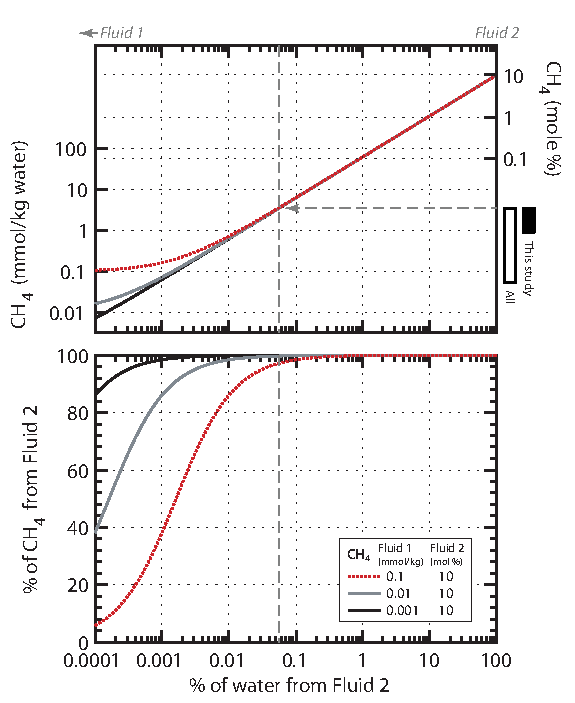
\includegraphics[width=0.65\linewidth]{figures/Fig3.6}
	\caption[Concentration of CH\textsubscript{4} in hydrothermal fluids upon mixing of a CH\textsubscript{4}-rich crustal fluid with a circulating, CH\textsubscript{4}-poor fluid]{%
		Composition
		of fluids formed by mixing of a CH\textsubscript{4}-poor
		actively-circulating seawater-derived hydrothermal fluid
		(\emph{Fluid~1}) with a CH\textsubscript{4}-rich fluid such as those
		observed in inclusions in plutonic rocks on the Southwest Indian Ridge
		and on the Mid-Atlantic Ridge (\emph{Fluid~2}) \parencite{Kelley_1996_JGR,Kelley_1997,Kelley+FruhGreen_1999_JGR}. Mixing curves are plotted for
		CH\textsubscript{4} concentrations in the \emph{Fluid~1} endmember
		ranging from 1 to 100~µmol/kg. Calculations assume that molalities of
		species other than CH\textsubscript{4} have a negligible effect on mole
		fractions in the high-CH\textsubscript{4} fluid. The black and white
		bars show CH\textsubscript{4} concentrations in vent fluids from this
		study (\autoref{tab:3:2}) and from mid-ocean ridge hydrothermal systems globally
		\parencite{Keir_2010_GRL}.
	}
	\label{fig:3:6}
\end{SCfigure*}









\textcite{Proskurowski++_2008_S} invoked abiotic reduction of aqueous
$\big\sum\!$CO\textsubscript{2} to explain the presence of high
(\textasciitilde{}1~mmol/kg) concentrations of CH\textsubscript{4} and
minor quantities (\textasciitilde{}1~µmol/kg or lower) of
C\textsubscript{2+} alkanes in vent fluids from the Lost City
hydrothermal field. They postulated a scenario that involves leaching of
primordial inorganic carbon from mantle host rocks, and subsequent
reduction of $\big\sum\!$CO\textsubscript{2} to CH\textsubscript{4} and
C\textsubscript{2+} in circulating fluids at relatively low temperature \parencite[\textless{}150~°C;][]{Proskurowski++_2006_CG}. However, Lost City
fluids contain vanishingly small amounts of $\big\sum\!$CO\textsubscript{2} because
the highly alkaline pH and high concentrations of Ca\textsuperscript{2+}
favor precipitation of carbonates, a process that proceeds rapidly at
temperatures experienced by the circulating fluids \parencite{Kelemen++_2011_AREarth,Grozeva++_2017_GCA}. The production of methane via
CO\textsubscript{2} reduction in an aqueous fluid depleted of
$\big\sum\!$CO\textsubscript{2} is therefore problematic in that it requires the addition of
mantle-derived CO\textsubscript{2} that is quickly reduced to form
CH\textsubscript{4} \parencite[up to 56\% conversion based on magmatic C/\textsuperscript{3}He ratios;][]{Proskurowski++_2008_S}, and the
remainder of which is then subsequently scavenged (presumably by
carbonate precipitation), leaving no evidence of its addition. Rates of
$\big\sum\!$CO\textsubscript{2} reduction must be comparable to or faster than
carbonate precipitation in order for CH\textsubscript{4} synthesis to
proceed in alkaline, $\big\sum\!$CO\textsubscript{2}-poor fluids such as those at
Lost City. Carbonate precipitation occurs rapidly during alteration of
peridotite \parencite{Grozeva++_2017_GCA}. In contrast, laboratory studies
consistently find sluggish reaction kinetics for the reduction of
$\big\sum\!$CO\textsubscript{2} to CH\textsubscript{4} in the presence and absence
of powdered peridotite or mafic mineral phases \parencite{McCollom+Seewald_2001_GCA,McCollom+Seewald_2003_GCA_formate,Seewald++_2006_GCA,Reeves_2010_thesis,McCollom_2016_PNAS,Grozeva++_2017_GCA}. Certain transition metal
catalysts can enhance rates of CH\textsubscript{4} production \parencite{Horita+Berndt_1999_S,Foustoukos+Seyfried_2004_S}, but H\textsubscript{2}
concentrations several orders of magnitude higher than those found in
vent fluids are required to render native Fe-Ni alloys stable \parencite{Frost_1985_JPet,Charlou++_2002_CG,Sleep++_2004_PNAS,McCollom+Bach_2009_GCA}. Furthermore, rates of CH\textsubscript{4} synthesis in fluids
deprived of $\big\sum\!$CO\textsubscript{2} are poorly-constrained, but generally
too low to be reliably detected on timescales of laboratory experiments \parencite{Fu++_2007_GCA,McCollom_2012_PNAS_comment,McCollom_2013_RiMG}.

Data from other vent fields are also inconsistent with synthesis of
CH\textsubscript{4} on timescales associated with actively-circulating
fluids. At the basalt-hosted Lucky Strike field, synthesis of methane
within the low-H\textsubscript{2} fluids discharging at the Medea and
Isabel vents is thermodynamically disfavored at \emph{in situ}
temperatures (270--292~°C; \autoref{tab:3:2} and \mrefs[D]{Fig.}{fig:3:3}). With increasing
temperature, methane formation becomes even more unfavorable (\mrefs[A]{Fig.}{fig:3:2}),
and thus aqueous CO\textsubscript{2} reduction at the higher
temperatures (possibly as high as 475~°C) the fluids have experienced
here \parencite{Pester++_2012_GCA} is also unsupported. Concentrations of
CH\textsubscript{4} shows no relation to either $\big\sum\!$CO\textsubscript{2} or
H\textsubscript{2} in the Lucky Strike fluids here \parencite[see discussion and Fig.~2 in][]{Pester++_2012_GCA}. These data indicate that
CH\textsubscript{4} did not form from reduction of $\big\sum\!$CO\textsubscript{2}
during migration of magmatic CO\textsubscript{2} between degassing from
the magma chamber at \textasciitilde{}3000~mbsf (meters below seafloor)
and venting at the seafloor. Taken together, this evidence suggests that
CH\textsubscript{4} originates not within an actively-convecting
hydrothermal fluid, but is produced elsewhere and entrained into the
circulating fluid.

The magmatic volatiles from which CH\textsubscript{4} forms may be
sourced from gabbroic rocks formed from cooling of volatile-bearing
melts beneath mid-ocean ridges. Oxidized carbon (as CO\textsubscript{2})
is generally considered to exhibit near-perfect incompatibility, such
that during decompression melting, nearly all carbon originally in the
suboceanic mantle partitions into the melt fraction, leaving very little
behind in residual peridotite. Estimates of the amount of carbon in the
mantle suffer from large uncertainties, but are typically in the range
of 20 to 300~ppm carbon \parencite{Dasgupta+Hirschmann_2010_EPSL}. Serpentinitized
oceanic peridotites from several mid-ocean ridges contain up to 1500~ppm
carbon, and are therefore a sink for carbon \parencite{Alt++_2013_L}. Carbon
in these rocks is thought to exist mostly as condensed phases \parencite{FruhGreen++_2004}, consistent with more recent observational and
theoretical considerations \parencite{Menez++_2012_NG,Pasini++_2013_L,Milesi++_2016_GCA}. In contrast, gabbros from the same areas contain
less carbon (up to 300~ppm), primarily hosted in inclusions bearing
CO\textsubscript{2}, CH\textsubscript{4} and/or graphite \parencite{FruhGreen++_1996_ODP-SR,Kelley+FruhGreen_1999_JGR,Kelley+FruhGreen_2001_GCA}.
These petrological constraints suggest that magmatic volatiles entrapped
in gabbros, but probably not fresh peridotites, are a potential source
for carbon in CH\textsubscript{4} at oceanic spreading centers.
Additionally, migration of magmatic volatiles out of melts directly into
layers of gabbro or peridotite may also enable carbon to come in contact
with reducing conditions conducive to methane synthesis.

The occurrence and composition of methane-rich aqueous fluids within the
sub-oceanic ridge lithosphere is recorded by secondary fluid inclusions
hosted in plutonic rocks. \textcite{Kelley_1996_JGR,Kelley_1997,Kelley+FruhGreen_1999_JGR} documented several types of abundant volatile-rich inclusions in
gabbros recovered from the slow-spreading Southwest Indian and
Mid-Atlantic Ridges by several Ocean Drilling Program (ODP) expeditions.
A common type of inclusion occurring along healed microcracks in
plagioclase grains contained up to 47\% CH\textsubscript{4} (with
balance of H\textsubscript{2}O). Temperatures indicated by
CO\textsubscript{2}--CH\textsubscript{4} carbon isotope geothermometry
(300--600~°C) and homogenization temperatures of the Southwest Indian
Ridge fluid inclusions (350--370~°C, corresponding to entrapment at
\emph{in situ} temperatures of ca.\ 400~°C) \parencite{Kelley+FruhGreen_1999_JGR}
agree with clumped isotopologue temperatures, and are compatible with
formation of CH\textsubscript{4} during re-speciation of occluded
magmatic volatiles as the host gabbros cooled to below 400~°C (\mrefs[A]{Fig.}{fig:3:2}).
While δ\textsuperscript{13}C values of CH\textsubscript{4} measured in
fluid inclusions are somewhat lower \parencite[$-$34 to $-$20‰;][]{Kelley+FruhGreen_1999_JGR} than observed values in vent fluids ($-$18 to $-$9‰; \autoref{tab:3:S1}), carbon isotopic data for inclusions may be affected by
potential background sources either endogenous to the crushed mineral
separates, introduced during sample handling, or formed during the
stepped heating experiments. These background sources of carbon typically
have relatively low δ\textsuperscript{13}C values of $-$25 to $-$30‰ \parencite{DesMarais_1986_EPSL,Miller+Pillinger_1997_GCA}.

Graphite is stable under conditions characterizing many hydrothermal
settings \parencite{Luque++_2009_G,Rumble_2014_E}. At isotopic equilibrium,
graphite is \textasciitilde{}10‰ enriched in \textsuperscript{13}C relative to
CH\textsubscript{4} at temperatures of 300 to 400~°C \parencite{Bottinga_1969_GCA}.
It is worth noting that in all mid-ocean ridge hydrothermal fluids,
δ\textsuperscript{13}C values of CH\textsubscript{4} are lower than
mantle-derived CO\textsubscript{2} ($-$5‰, \mrefs[A]{Fig.}{fig:3:1}). Relatively uniform
δ\textsuperscript{13}C values ($-$19‰ to $-$9‰) are observed in vent fluids
with high (millimolar) CH\textsubscript{4} contents \parencite{McCollom+Seewald_2007_CR,Keir_2010_GRL}. Furthermore,
CH\textsubscript{4}/\textsuperscript{3}He ratios in vent fluids \parencite[see][]{Keir_2010_GRL} indicate less-than-quantitative conversion
(\textasciitilde{}0.2\% to 50\%) of mantle carbon to CH\textsubscript{4}
 \parencite[C/\textsuperscript{3}He \textasciitilde{} 1×10\textsuperscript{9},][]{Marty+Tolstikhin_1998_CG}. Precipitation of graphite from a
CH\textsubscript{4}-rich fluid entrapped in plutonic rocks may explain
both the missing carbon \parencite{McDermott++_2015_PNAS} and the observed
δ\textsuperscript{13}C values \parencite{Luque++_2012_GFront}.

\autoref{fig:3:S1} shows predictions from a thermodynamic model of an
ideal graphite-saturated C--O--H vapor with oxygen fugacity given by the
fayalite-magnetite-quartz (FMQ) mineral buffer assemblage and a total
pressure of 1~kbar. Calculations show that precipitation of graphite
concomitant with methane formation is favored at ca.\ 400~°C and under
water-poor conditions, consistent with many previous investigations \parencite{French_1966_RG,Eugster+Skippen_1967,Ohmoto+Kerrick_1977_AJS,Holloway_1984_G,FruhGreen++_2004}. Predicted
C\textsubscript{1}/C\textsubscript{2} ratios are also consistent with
measured values in vent fluids \parencite[][and \autoref{fig:3:S1}]{McDermott_2015_thesis}.
Propane (C\textsubscript{3}) is in excess by two orders of magnitude
compared with thermodynamic equilibrium at \textasciitilde{}300~°C
\parencite[][and \autoref{fig:3:S1}]{McDermott_2015_thesis}. To explain the relative
proportions of ethane and propane (and butanes) at this temperature
requires both a high CH\textsubscript{4} fugacity and (paradoxically) a
low H\textsubscript{2} fugacity of several log units below (more
oxidized than) FMQ. Generation of small amounts of C\textsubscript{2+}
hydrocarbons (\textasciitilde{}1~µM or less) from the thermal breakdown
of dissolved organic matter carried in recharging seawater
(\textasciitilde{}40~µM) may account for the excess propane and butanes
relative to ethane and methane. Alternatively, the C\textsubscript{2+}
hydrocarbons may not have equilibrated at a uniform temperature
\parencite{McDermott_2015_thesis}, or may be formed via low-yield, kinetically-throttled
reactions occurring in circulating fluids \parencite{Foustoukos+Seyfried_2004_S}. Regardless of their specific origins, similarities in the
abundances and isotopic compositions of low molecular weight
hydrocarbons in vent fluids at Von Damm and other hot-spring systems at
slow-spreading ridges suggest that they may share common origins.

Concentrations of CH\textsubscript{4} in the gabbro-hosted inclusions
from the Southwest Indian Ridge and from other slow-spreading areas can
be several orders of magnitude greater than those observed in
corresponding vent fluids \parencite{Kelley_1996_JGR,Kelley_1997}. Mass-balance
considerations suggest that extraction of CH\textsubscript{4}-rich
fluids occluded in gabbros can explain CH\textsubscript{4}
concentrations at all known sediment-free mid-ocean ridge hydrothermal
fields. Mixing curves plotted in \autoref{fig:3:6} show that addition of less than
0.1\% of a CH\textsubscript{4}--H\textsubscript{2}O fluid of similar
composition to those indicated by the inclusions (\emph{Fluid 2} in the
figure) to a CH\textsubscript{4}-poor circulating hydrothermal fluid
(\emph{Fluid 1}) is sufficient to match even the highest
CH\textsubscript{4} concentrations seen in vent fluids. Assuming carbon
contents ranging from 30 to 300~ppm in the gabbro \parencite{Kelley+FruhGreen_1999_JGR}, water-to-rock ratios between 0.8 and 8 are required
to explain CH\textsubscript{4} concentrations of up to 3~mmol/kg in vent
fluids assuming all carbon in gabbro existed as leachable
CH\textsubscript{4}. Lower water-to-rock ratios are necessary if
conversion efficiency is less than 100\% (e.g., due to graphite
precipitation) or if lower initial carbon contents are assumed.
Constraints from mobile inorganic elements (e.g., Li, Rb, Sr) generally
indicate that water/rock ratios are substantially lower than
\textasciitilde{}10 in many mid-ocean ridge hydrothermal systems \parencite{VonDamm++_1985_GCA_EPR,Berndt++_1989_GCA} with values of 0.4 to 6
calculated for the subsurface at Von Damm \parencite{McDermott_2015_thesis} and 2 to 4
at Lost City  \parencite{Foustoukos++_2008_GCA} for example.


While only slow-spreading environments were investigated in this study,
we hypothesize that the same origin of methane applies at sites on the
fast-spreading East Pacific Rise, particularly given the similar
δ\textsuperscript{13}C values of methane there \parencite{Welhan+Craig_1983}.
The fact that these hydrothermal fluids contain low C\textsubscript{2+}
along with low CH\textsubscript{4} concentrations \parencite{Keir_2010_GRL,Welhan_1988_CG} suggests a genetic link between CH\textsubscript{4} and the
C\textsubscript{2+} hydrocarbons. Differences in axial structure and
tectonism may account for the difference in hydrocarbon content of vent
fluids at fast- and slow-spreading ridges. At magma-poor slow-spreading
ridges, extension is accommodated primarily by detachment faulting, as
opposed to magmatic emplacement of new crust that characterizes
fast-spreading ridges \parencite{Buck++_2005_N,Dunn_2007_TiG}. Low-angle,
large-offset, and long-lived (\textgreater{}1 Myr) normal faults near
vent fields at slow-spreading ridges allow for fluid penetration deep
into plutonic rocks of layer 3, enabling access to fresh gabbroic
material and/or inclusions to be leached \parencite{Kelley_1996_JGR,Schroeder++_2002_G,Schlindwein+Schmid_2016_N}. In contrast, in fast spreading
environments such as the East Pacific Rise, shallow melt lenses at 1 to
2~km below seafloor may limit the depth of circulation \parencites(e.g.,)()[][]{Hasenclever++_2014_N}[and references in][]{Alt_1995_AGU-GM}.

\section{Conclusions}\label{conclusions}

Methane clumped isotopologue data obtained for fluids venting from
diverse unsedimented mid-ocean ridge hydrothermal systems uniformly
indicate temperatures of last equilibration of ca.\ 300~°C. Taken in
combination with geochemical and geologic observations and reaction
rates determined in experiments, the
Δ\textsuperscript{13}CH\textsubscript{3}D data provide evidence that
abiotic reduction of $\big\sum\!$CO\textsubscript{2} at
low temperatures (\textless{}200~°C) is not a significant source of
methane over timescales characterizing convective hydrothermal
circulation at oceanic spreading centers. Furthermore, consideration of
volatile contents and C--O--H speciation in melt-derived plutonic rocks
and residual peridotites suggests that temperature, pressure,
\(f_{\mathrm{O}_{\mathrm{2}}}\), and
\(f_{\mathrm{H}_{\mathrm{2}}\mathrm{O}}\) conditions conducive to
methane synthesis may be widespread in the oceanic crust.

Two hypotheses were considered for explaining the origin of
CH\textsubscript{4} in hydrothermal fluids: (\emph{i}) aqueous synthesis
of CH\textsubscript{4} during active circulation and (\emph{ii})
extraction of CH\textsubscript{4}-rich fluids occluded in plutonic
rocks. While both are conceivably compatible with the methane
isotopologue data when taken in isolation, clumped isotopologue
temperatures indicate that formation of CH\textsubscript{4} from
$\big\sum\!$CO\textsubscript{2} at Lost City does not occur at temperatures
\textless{}200~°C in the upflow. Furthermore, the former scenario is not
compatible with thermodynamic, radioisotopic, and mass balance
constraints at several sites. These lines of evidence lead us to favor
the latter hypothesis, which invokes a more straightforward scenario
wherein vent fluids with millimolar quantities of CH\textsubscript{4}
represent mixtures of a minute amount of a CH\textsubscript{4}-rich
fluid (of hypogene origin) with a large volume of an
actively-circulating, CH\textsubscript{4}-poor fluid. Proportions of
mixing may be determined by the relative access that circulating fluids
have to magmatic volatile-bearing rocks of the plutonic foundation. This
could also explain apparent relationships of CH\textsubscript{4}
concentration in vent fluids to tectonic setting and host rock
lithology. Efforts to distinguish between the CH\textsubscript{4}
contributed via these pathways will benefit from rigorous interrogation
of factors governing fluid flow and chemical kinetics in
hydrothermally-influenced settings.

The new data also provide constraints on the closure temperature of
hydrogen exchange between methane and water. The observation of sluggish
or indiscernible exchange of H among methane isotopologues below ca.
270~°C on timescales of \textasciitilde{}10\textsuperscript{2}~years is
relevant not only to the application of clumped isotope measurements as
a novel geothermometer, but also provides information about the
stability of the C--H bond in hydrocarbons in nature. Given the
increasing appreciation of hydrocarbon-water-mineral interactions in
economically important settings \parencite{Seewald_2003_N}, insights of this nature
may find utility in studies of the origin and composition of aqueous and
organic fluids in the Earth's subsurface.

\section*{Acknowledgments}\label{acknowledgments-1}

We thank Frieder Klein, Wolfgang Bach, and Grant Garven for helpful
discussions regarding the petrology and plumbing of hydrothermal
systems. Grants from the National Science Foundation (NSF EAR-1250394 to
S.O.), NASA Astrobiology Institute (NAI \#024461), N. R. Braunsdorf and D. J. H.
Smit of Shell PTI/EG and the Deep Carbon Observatory (to S.O.) supported
this work. S.O. thanks the Kerr-McGee Professorship at MIT. This
research was conducted with Government support under and awarded by U.S.
Department of Defense, Office of Naval Research, National Defense
Science and Engineering Graduate (NDSEG) Fellowship (to D.T.W.), 32 CFR
168a. D.T.W. was also supported via a Shell-MITEI fellowship.


\begin{figure*}
	\centering
	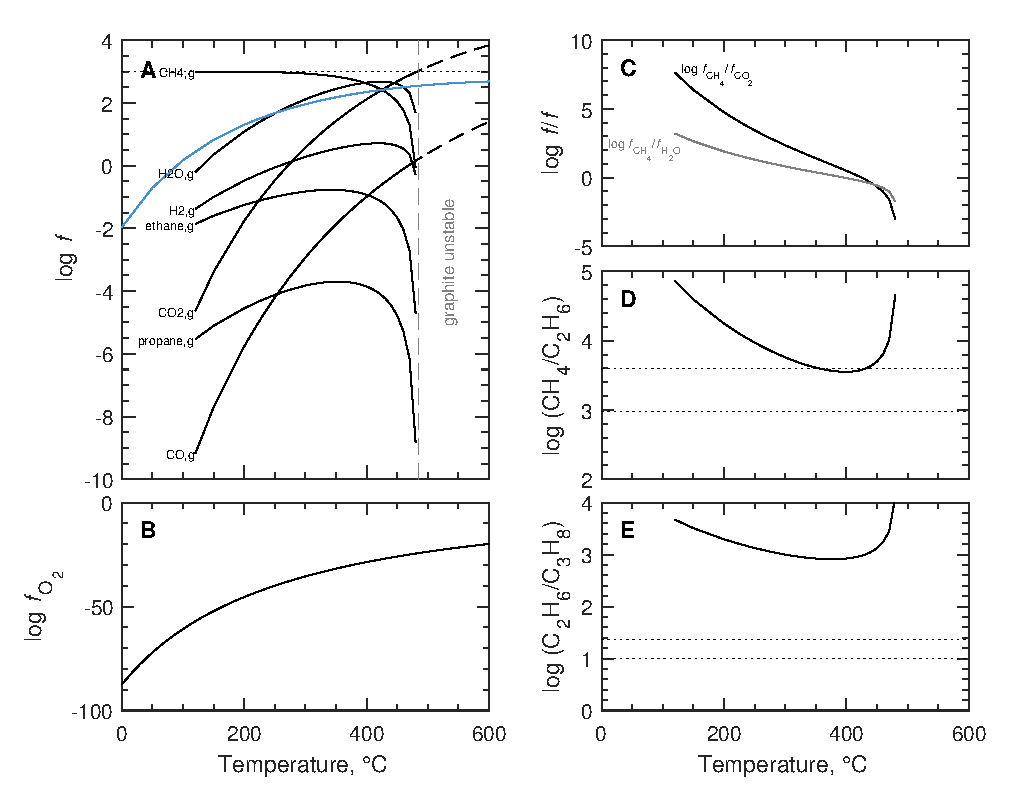
\includegraphics[width=0.95\linewidth]{figures/Fig3.S1}
	\caption[Equilibrium composition of a graphite-saturated C--O--H fluid at 1000~bar with \(f_{\mathrm{O}_{\mathrm{2}}}\) = FMQ]{Equilibrium composition of a
		graphite-saturated C--O--H fluid at 1000~bar (\textbf{A}) with oxygen
		fugacity (\(f_{\mathrm{O}_{\mathrm{2}}}\)) given by the
		fayalite-magnetite-quartz (FMQ) redox buffer (\textbf{B}). The modeled
		fluid is an ideal gas consisting of CO, CO\textsubscript{2},
		H\textsubscript{2}, H\textsubscript{2}O, O\textsubscript{2}, ethane, and
		propane. The model is essentially that of \textcite{French_1966_RG}, with the addition of C\textsubscript{2+} compounds (as also considered by \textcite{Kawagucci++_2013_CG,McDermott_2015_thesis}, with different assumptions regarding redox, water activity, and total mass of carbon). To calculate the
		composition of the fluid, equilibrium constants were computed at various
		temperatures using CHNOSZ \parencite{Dick_2008_GT} from tabulated standard molal
		thermodynamic properties and equation of state parameters \parencite{CHNOSZ_Kel60,CHNOSZ_HDN+78,CHNOSZ_HOK+98,CHNOSZ_WEP+82,Johnson++_1992_CnG,CHNOSZ_Sho93}, the fugacities of CO and CO\textsubscript{2} were
		calculated, and then the fugacities of all other gaseous species were
		solved iteratively under the constraint that $\big\sum\!$\emph{f} = 1000~bar \parencite[a
		pressure typical of those indicated by fluid inclusion studies;][]{Vanko_1988_JGR}. Graphite is unstable above \textasciitilde{}500~°C, as shown
		by the equilibrium fugacities of CO+CO\textsubscript{2} exceeding the
		pressure of the system (dashed lines in A). Ratios of fugacities of
		selected species show that CH\textsubscript{4} is the dominant gas-phase
		species below \textasciitilde{}400~°C (\textbf{C}), and that predicted
		ratios of C\textsubscript{1}/C\textsubscript{2} and
		C\textsubscript{2}/C\textsubscript{3} are
		\textasciitilde{}10\textsuperscript{3} to 10\textsuperscript{4} between
		200 and 400~°C (\textbf{D}, \textbf{E}). Dotted lines in (D) and (E)
		mark the range of C\textsubscript{1}/C\textsubscript{2} and
		C\textsubscript{2}/C\textsubscript{3} measured in hydrothermal fluids
		from the four vent fields we studied \parencite{Charlou++_2000_CG,Charlou++_2002_CG,Proskurowski++_2008_S,McDermott++_2015_PNAS}. The vapor pressure
		curve of water at 1000~bar is shown in blue in (A). Values of
		\(\log f_{\mathrm{H}_{\mathrm{2}}\mathrm{O}}\) that plot above this
		curve are inaccessible because the presence of liquid water sets the
		fugacity of H\textsubscript{2}O and causes the fugacities of
		O\textsubscript{2} and all other species to adjust accordingly.
		Therefore, values of
		\(\log\left({f_{\mathrm{C}\mathrm{H}_{\mathrm{4}}}}\middle/{f_{\mathrm{H}_{\mathrm{2}}\mathrm{O}}}\right) > 0\)
		do not necessarily indicate that total CH\textsubscript{4} content
		exceeds total water content when multiple fluid phases coexist. Liquid
		water has been neglected in our model, but calculations in which
		H\textsubscript{2}O(\emph{l}) is explicitly considered show that
		graphite, an H\textsubscript{2}O-dominated liquid, and a
		CH\textsubscript{4}-rich gas phase can coexist at
		\textasciitilde{}400~°C and \(f_{\mathrm{O}_{\mathrm{2}}}\) close to FMQ
		\parencite{Holloway_1984_G}.}
	\label{fig:3:S1}
\end{figure*}





\begin{figure*}
	\centering
	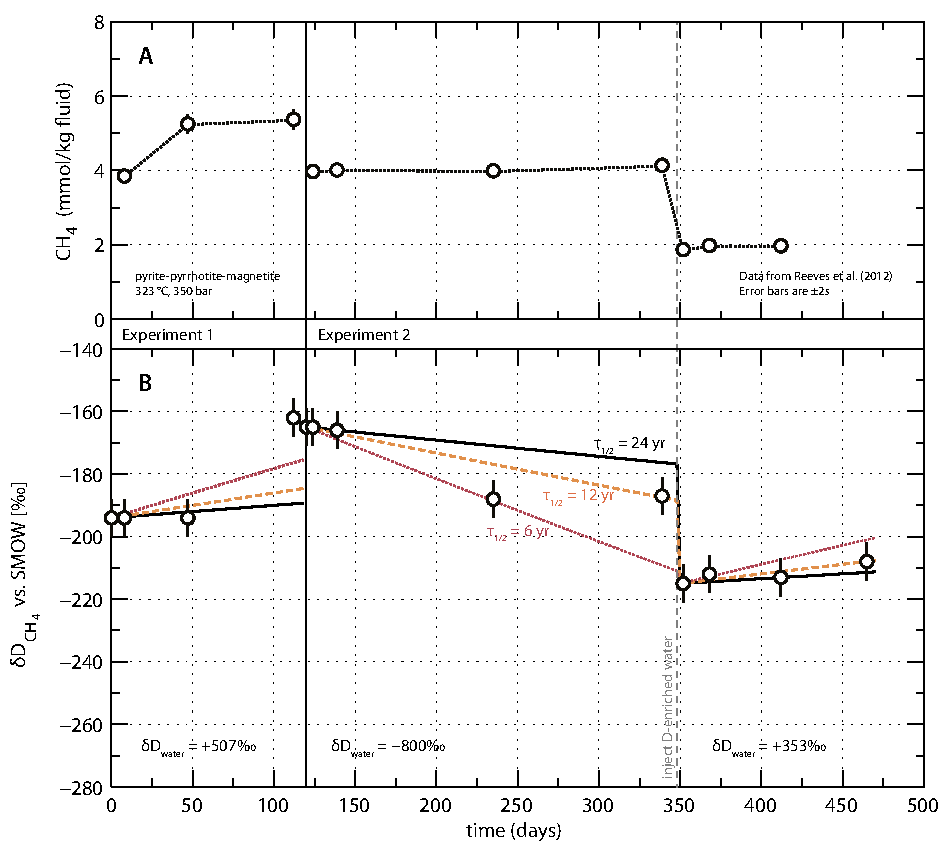
\includegraphics[width=0.95\linewidth]{figures/Fig3.S2}
	\caption[Rates of hydrogen exchange between CH\textsubscript{4}(\emph{aq}) and
	H\textsubscript{2}O(\emph{l}) from data of \textcite{Reeves++_2012_GCA} ]{%
		Experimental constraints on hydrogen
		exchange between CH\textsubscript{4}(\emph{aq}) and
		H\textsubscript{2}O(\emph{l}) from two experiments conducted by \textcite{Reeves++_2012_GCA} in a flexible cell hydrothermal apparatus at 323~°C and
		350~bar. Concentrations of CH\textsubscript{4} (\textbf{A}) remain
		indistinguishable within analytical error (±5\%, 2\emph{s}) in
		Experiment~2, but not in Experiment~1, perhaps due to calibration or operator error as noted by those authors. Measured
		pH was \textasciitilde{}4.2, and concentrations of H\textsubscript{2}
		and $\big\sum\!$H\textsubscript{2}S were 0.26--0.7 mmol/kg fluid and
		\textasciitilde{}11~mmol/kg fluid, respectively, consistent with
		predictions for a Fe--S--O--H fluid buffered by PPM at experimental
		conditions \parencite{Reeves++_2012_GCA}. Panel (\textbf{B}) shows measurements
		of D/H of CH\textsubscript{4} compared against modeled kinetics for D/H
		exchange with varying half-exchange time ($\tau_{1/2} = \ln(2)/k$). The modeled kinetics assume that CH\textsubscript{4}
		concentration is constant, the rate of isotopic exchange is first order
		in CH\textsubscript{4}, and the equilibrium D/H fractionation factor
		{[}$\varepsilon = $ (D/H)\textsubscript{methane}/(D/H)\textsubscript{water} -- 1{]} is
		$-$130‰ (see \autoref{fig:3:5}). We take $\tau_{1/2}$ = 24~yr (black curve)
		as a best-guess estimate of the rate of true isotopic exchange; this
		value is shown in \autoref{fig:3:4}.
	}
	\label{fig:3:S2}
\end{figure*}






\begin{landscape}	
	
	\centering
	
	\begin{ThreePartTable}	
			
		\begin{TableNotes}
			\item Abbreviations: mm, mmol/kg fluid; mM, mmol/L fluid.
			
			\item Data sources: (1) this study; (2) \textcite{Reeves++_2014_PNAS}; (3) \textcite{Charlou++_2010}; (4) \textcite{Proskurowski++_2006_CG}; (5) \textcite{Welhan+Craig_1983};
			(6) \textcite{Horibe+Craig_1995_GCA}; (7) \textcite{Kawagucci++_2010_JGR}; (8) \textcite{Kumagai++_2008_Gf}; (9) \textcite{McDermott++_2015_PNAS}.
			
			\item Notes: † cf. \emph{T}\textsubscript{max} 96~°C in ref.~2; ‡ phase-separated; § snail colony; ¶ shrimp colony
			
			\item \textsuperscript{a} Dash (---) indicates that data were not reported or
			that samples were unable to be matched across multiple references.
			
			\item \textsuperscript{b} Maximum measured vent temperature.
			
			\item \textsuperscript{c} Asterisk (*) indicates near-endmember fluid sample
			(represented by stars in \autoref{fig:3:5}). For these samples, concentrations of
			$\big\sum\!$CO\textsubscript{2}, H\textsubscript{2}, and CH\textsubscript{4} and
			δ\textsuperscript{13}C values of $\big\sum\!$CO\textsubscript{2} have been
			extrapolated to endmember fluid composition (regressed to zero Mg
			content) assuming entrainment of seawater containing \textasciitilde{}53~mM Mg.
			
			\item \textsuperscript{d} Endmember vent fluids typically have δD values of
			H\textsubscript{2}O between $-$2 and +4‰ \parencite{Shanks++_1995_AGU-GM}. A value of
			0‰ was assumed when no data could be found (see text and \autoref{fig:3:5}).
			
			\item \textsuperscript{e} Values are as reported; it is not known whether
			correction for $\big\sum\!$CO\textsubscript{2} in seawater was applied.
			
		\end{TableNotes}
		
		\setlength{\tabcolsep}{10pt}
		\setlength{\abovetopsep}{9pt}
		\small
		
		\begin{longtable}[]{@{} ll d{0}l lll ll @{\hskip 0.2em} p{0.01em} lll l @{}}
			
			\tabularnewline  % adds padding!
			\tabularnewline
			\caption[Compilation of δD values of \ce{CH4} \& \ce{H2} and associated data]{Compilation of hydrogen isotope ratios of CH\textsubscript{4} and
				H\textsubscript{2} and associated data on vent fluids from sediment-poor
				hydrothermal systems.}\label{tab:3:S1}\\ 	% this \\ is very important !!
			\toprule
			\multirow{2}{*}{Field} & \multirow{2}{*}{Vent}  & \multirow{2}{*}{\shortstack[l]{\emph{T}\textsubscript{max}\\ (°C)\textsuperscript{b}}}  & \multirow{2}{*}{\shortstack[l]{Mg\\ (mM)}}  & \multirow{2}{*}{\shortstack[l]{$\big\sum\!$\ce{CO2}\\ (mm)}}  & \multirow{2}{*}{\shortstack[l]{\ce{H2}\\ (mM)}}  & \multirow{2}{*}{\shortstack[l]{\ce{CH4}\\ (mM)}} & \multicolumn{2}{c}{δ\textsuperscript{13}C (‰)} & & \multicolumn{3}{c}{δD (‰)} & \multirow{2}{*}{Notes}\tabularnewline
			\cmidrule{8-9} \cmidrule{11-13}
			 &  &  &   &   &   &   & $\big\sum\!$CO\textsubscript{2} & CH\textsubscript{4} & &
			CH\textsubscript{4} & H\textsubscript{2} &
			H\textsubscript{2}O\textsuperscript{d} &\tabularnewline
			\midrule
			\endfirsthead
%
			\tabularnewline
			\tabularnewline			
			\caption[]{Compilation of hydrogen isotope ratios of CH\textsubscript{4} and
				H\textsubscript{2} and associated data (\textit{continued}).}\\ 	% this \\ is very important !!
			\toprule
			\multirow{2}{*}{Field} & \multirow{2}{*}{Vent}  & \multirow{2}{*}{\shortstack[l]{\emph{T}\textsubscript{max}\\ (°C)\textsuperscript{b}}}  & \multirow{2}{*}{\shortstack[l]{Mg\\ (mM)}}  & \multirow{2}{*}{\shortstack[l]{$\big\sum\!$\ce{CO2}\\ (mm)}}  & \multirow{2}{*}{\shortstack[l]{\ce{H2}\\ (mM)}}  & \multirow{2}{*}{\shortstack[l]{\ce{CH4}\\ (mM)}} & \multicolumn{2}{c}{δ\textsuperscript{13}C (‰)} & & \multicolumn{3}{c}{δD (‰)} & \multirow{2}{*}{Notes}\tabularnewline
			\cmidrule{8-9} \cmidrule{11-13}
			 &  &  &   &   &   &   & $\big\sum\!$CO\textsubscript{2} & CH\textsubscript{4} & &
			CH\textsubscript{4} & H\textsubscript{2} &
			H\textsubscript{2}O\textsuperscript{d} &\tabularnewline
			\midrule
			\endhead
			
			\midrule
			\multicolumn{14}{r}{\textit{Continued on next page}}
			\tabularnewline
			\tabularnewline
			\endfoot
%			\begin{minipage}[b]{0.07\columnwidth}\raggedright\strut
%				Field\strut
%			\end{minipage} & \begin{minipage}[b]{0.07\columnwidth}\raggedright\strut
%				Vent\textsuperscript{a}\strut
%			\end{minipage} & \begin{minipage}[b]{0.07\columnwidth}\raggedright\strut
%				\emph{T}\textsubscript{max}
%				
%				(°C)\textsuperscript{b}\strut
%			\end{minipage} & \begin{minipage}[b]{0.07\columnwidth}\raggedright\strut
%				Mg
%				
%				(mM)\textsuperscript{c}\strut
%			\end{minipage} & \begin{minipage}[b]{0.07\columnwidth}\raggedright\strut
%				$\big\sum\!$CO\textsubscript{2}
%				
%				(mm)\strut
%			\end{minipage} & \begin{minipage}[b]{0.07\columnwidth}\raggedright\strut
%				H\textsubscript{2}
%				
%				(mM)\strut
%			\end{minipage} & \begin{minipage}[b]{0.07\columnwidth}\raggedright\strut
%				CH\textsubscript{4}
%				
%				(mM)\strut
%			\end{minipage} & \begin{minipage}[b]{0.07\columnwidth}\raggedright\strut
%				δ\textsuperscript{13}C (‰)\strut
%			\end{minipage} & \begin{minipage}[b]{0.07\columnwidth}\raggedright\strut
%				\strut
%			\end{minipage} & \begin{minipage}[b]{0.07\columnwidth}\raggedright\strut
%				δD (‰)\strut
%			\end{minipage} & \begin{minipage}[b]{0.07\columnwidth}\raggedright\strut
%				Notes\strut
%			\end{minipage}\tabularnewline
%			
%			& & & & & & & $\big\sum\!$CO\textsubscript{2} & CH\textsubscript{4} & &
%			CH\textsubscript{4} & H\textsubscript{2} &
%			H\textsubscript{2}O\textsuperscript{d} &\tabularnewline
%			& & & & & & & & & & & & &\tabularnewline
			
			\insertTableNotes\\
			\endlastfoot
			
			&\tabularnewline
			\multicolumn{5}{@{}l}{\textit{Mid-Atlantic Ridge}}  & & & &\tabularnewline
			Rainbow & Guillaume (X4) & 361 & 0* & 24.3 & 16.5 & 2.13 & --- & $-$17.6 &
			& $-$98 & --- & --- & (1, 2)\tabularnewline
			& CMSP\&P & 365 & 0* & 21.9 & 15.9 & 2.05 & --- & $-$17.5 & & $-$98 & --- &
			--- & (1, 2)\tabularnewline
			& Auberge (X3) & 370 & 0* & 22.8 & 15.7 & 2.16 & --- & $-$17.4 & & $-$98 &
			--- & --- & (1, 2)\tabularnewline
			& --- & 365 & 0* & 16 & 16 & 2.5 & $-$3.2\textsuperscript{e} & $-$17.7 & &
			$-$105 & $-$356 & --- & (3)\tabularnewline
			& --- & 360 & 0* & 17 & 13 & 1.6 & $-$2.5\textsuperscript{e} & $-$17.8 & &
			$-$107 & $-$379 & --- & (3)\tabularnewline
			Lost City & Beehive & 94 & 0* & 0.18 & 10.4 & 1.08 & --- & $-$10.9 & &
			$-$127 & --- & --- & (1, 2)\tabularnewline
			& & 90 & 0* & --- & --- & --- & --- & --- & & $-$127 & $-$609 & +2 to 7 &
			(4)\tabularnewline
			& & 90 & 0* & --- & --- & --- & --- & --- & & $-$126 & $-$609 & +2 to 7 &
			(4)\tabularnewline
			& Marker 6 & 67 & 0* & --- & --- & --- & --- & --- & & $-$108 & $-$605 & +2
			to 7 & (4) {†}\tabularnewline
			& & 62 & 0* & --- & --- & --- & --- & --- & & $-$129 & $-$616 & +2 to 7 &
			(4) {†}\tabularnewline
			& IMAX (IF) & 55 & --- & --- & --- & --- & --- & --- & & $-$129 & $-$649 &
			+2 to 7 & (4)\tabularnewline
			& & 55 & --- & --- & --- & --- & --- & --- & & $-$139 & $-$646 & +2 to 7 &
			(4)\tabularnewline
			& & 55 & --- & --- & --- & --- & --- & --- & & $-$136 & $-$648 & +2 to 7 &
			(4)\tabularnewline
			& Marker 7 & 28 & --- & --- & --- & --- & --- & --- & & $-$129 & $-$663 & +2
			to 7 & (4)\tabularnewline
			& & 28 & --- & --- & --- & --- & --- & --- & & $-$125 & $-$666 & +2 to 7 &
			(4)\tabularnewline
			& Marker 8 & 43 & --- & --- & --- & --- & --- & --- & & $-$141 & $-$658 & +2
			to 7 & (4)\tabularnewline
			& & 43 & --- & --- & --- & --- & --- & --- & & $-$136 & $-$651 & +2 to 7 &
			(4)\tabularnewline
			& Marker C & 62 & --- & --- & --- & --- & --- & --- & & $-$126 & $-$620 & +2
			to 7 & (4)\tabularnewline
			& & 70 & --- & --- & --- & --- & --- & --- & & $-$130 & $-$614 & +2 to 7 &
			(4)\tabularnewline
			& Marker H & 60 & --- & --- & --- & --- & --- & --- & & $-$99 & $-$657 & +2
			to 7 & (4)\tabularnewline
			& & 60 & --- & --- & --- & --- & --- & --- & & $-$104 & $-$689 & +2 to 7 &
			(4)\tabularnewline
			& Marker 3 & 61 & --- & --- & --- & --- & --- & --- & & $-$112 & $-$610 & +2
			to 7 & (4)\tabularnewline
			& & 71 & --- & --- & --- & --- & --- & --- & & $-$103 & $-$605 & +2 to 7 &
			(4)\tabularnewline
			& & 73 & --- & --- & --- & --- & --- & --- & & $-$125 & $-$609 & +2 to 7 &
			(4)\tabularnewline
			& --- & 93 & 0* & --- & --- & --- & --- & $-$11.9 & & $-$130 & $-$618 & --- &
			(3)\tabularnewline
			
%			&\tabularnewline
			Broken Spur & --- & 353 & 0* & --- & --- & --- & --- & --- & & --- &
			$-$393 & --- & (4)\tabularnewline
			\tabularnewline
			Logatchev (1?) & --- & 350 & 0* & --- & --- & --- & --- & --- & & $-$109 & $-$372
			& --- & (4)\tabularnewline
			Logatchev 1 & --- & 346 & 0* & 3.6 & 9 & 2.0 & +4.1\textsuperscript{e} &
			$-$10.2 & & $-$104 & $-$350 & --- & (3)\tabularnewline
			& --- & 352 & 0* & 4.4 & 13 & 2.6 & +7.4\textsuperscript{e} & $-$10.3 & &
			$-$104 & $-$360 & --- & (3)\tabularnewline
			Logatchev 2 & --- & 320 & 0* & 6.2 & 11 & 1.2 & +9.5\textsuperscript{e}
			& $-$6.1 & & $-$93 & $-$231 & --- & (3) {‡}\tabularnewline
			Ashadze 1 & --- & 353 & 0* & 3.7 & 8 & 0.5 & +2.1\textsuperscript{e} &
			$-$12.3 & & $-$104 & $-$333 & --- & (3)\tabularnewline
			& --- & 353 & 0* & --- & 19 & 1.2 & +4.6\textsuperscript{e} & $-$14.1 & &
			$-$101 & $-$343 & --- & (3)\tabularnewline
			Ashadze 2 & --- & 296 & 0* & --- & 26 & 0.8 & +0.2\textsuperscript{e} &
			$-$8.7 & & $-$107 & $-$270 & --- & (3) {‡}\tabularnewline
			Lucky Strike & Medea & 270 & 0* & 98 & 0.063 & 0.89 & --- & $-$14.2 & &
			$-$99 & --- & --- & (1, 2)\tabularnewline
			& Isabel & 292 & 0* & 112 & 0.034 & 0.86 & --- & $-$12.6 & & $-$100 & --- &
			--- & (1, 2)\tabularnewline
			& & & & & & & & & & & & &\tabularnewline
			\multicolumn{5}{@{}l}{\textit{East Pacific Rise}} & &  & & &\tabularnewline
			9° N & --- & 380 & 0* & --- & --- & --- & --- & --- & & --- & $-$328 & ---
			& (4)\tabularnewline
			21° N & Nat. Geo. Soc. & 350 & 0* & --- & 30.5 & 1.4 & $-$7.0 & $-$15.0 & &
			$-$102 & $-$401 & +0.5 & (5, 6)\tabularnewline
			& & & & & & & & & & & & &\tabularnewline
			\multicolumn{5}{@{}l}{\textit{Central Indian Ridge}}  & & & &\tabularnewline
			Kairei & Kali & 362 & 0* & 8.0 & 3.3 & 0.12 & $-$5.3 & $-$9.8 & & --- & $-$368
			& --- & (7, 8)\tabularnewline
			& & 316 & 8.4 & 12.1 & 3.6 & --- & --- & --- & & --- & $-$328 & --- & (7,
			8)\tabularnewline
			& Monju & 299 & 5.2 & 7.9 & 2.1 & --- & --- & --- & & --- & $-$385 & --- &
			(7, 8)\tabularnewline
			& & 42 & 50.9 & 9.3 & 8×10\textsuperscript{$-$4} & --- & --- & --- & & ---
			& $-$431 & --- & (7, 8)\tabularnewline
			& & 87 & 43.7 & 6.0 & 0.69 & --- & --- & --- & & --- & $-$361 & --- & (7,
			8) {§} \tabularnewline
			& & 22 & 48.3 & 12.6 & 0.13 & --- & --- & --- & & --- & $-$493 & --- & (7,
			8) {§}\tabularnewline
			& Fugen & 305 & 4.5 & 9.5 & 2.7 & --- & --- & --- & & --- & $-$391 & --- &
			(7, 8)\tabularnewline
			& Daikoku  & 306 & 0* & --- & 2.2 & --- & --- & --- & & --- &
			$-$340 & --- & (7)\tabularnewline
			& --- & 350 & 0* & --- & --- & --- & --- & --- & & --- & $-$400 & --- &
			(4)\tabularnewline
			Edmond & Nura Nura & 375 & 0* & 12.8 & 0.11 & 0.31 & $-$5.5 & $-$13.5 & &
			--- & $-$362 & --- & (7, 8)\tabularnewline
			& Marker 27 & 325 & 0* & 12.3 & 0.10 & --- & --- & --- & & --- & $-$377 &
			--- & (7, 8)\tabularnewline
			& White Head & 263 & 12.4 & 8.1 & 0.04 & --- & --- & --- & & --- & $-$412
			& --- & (7, 8)\tabularnewline
			& Gr.\ Shrimp V.\ & 281 & 13.4 & 12.1 & 0.48 & --- & --- & --- & &
			--- & $-$681 & --- & (7, 8) {¶} \tabularnewline
			& Marker 24 & 116 & 40.6 & 8.7 & 0.07 & --- & --- & --- & & --- & $-$476 &
			--- & (7, 8)\tabularnewline
			& & & & & & & & & & & & &\tabularnewline
			\multicolumn{5}{@{}l}{\textit{Mid-Cayman Rise}}  & & & & &\tabularnewline
			Von Damm & Old Man Tree & 115 & 14.0 & 1.80 & 10.5 & 1.97 & --- & $-$16.2
			& & $-$107 & --- & --- & (1, 9)\tabularnewline
			& Ravelin 1 & 145 & 15.0 & 2.52 & 13.4 & 2.02 & --- & $-$16.4 & & $-$107 &
			--- & --- & (1, 9)\tabularnewline
			& East Summit & 226 & 0* & 2.80 & 18.2 & 2.81 & --- & $-$16.4 & & $-$107 &
			--- & --- & (1, 9)\tabularnewline
			& & & & & & & & & & & & &\tabularnewline
			\bottomrule
		\end{longtable}
	
	\end{ThreePartTable}

\end{landscape}






	\chapter{\texorpdfstring{Fractionation of the methane isotopologues
		\textsuperscript{13}CH\textsubscript{4},
		\textsuperscript{12}CH\textsubscript{3}D, and
		\textsuperscript{13}CH\textsubscript{3}D during aerobic oxidation of
		methane by \emph{Methylococcus capsulatus} (Bath)
	}{Fractionation of the methane isotopologues 13CH4, 12CH3D, and 13CH3D during aerobic oxidation of methane by Methylococcus capsulatus (Bath) }}\label{ch:4}
%\chaptermark{Fractionation of methane isotopologues by {\protect\textit{M.\ capsulatus}}}
\chaptermark{Aerobic oxidation of methane}

\begin{abstract}

\noindent Aerobic oxidation of methane plays a major role in reducing the amount
of methane emitted to the atmosphere from freshwater and marine
settings. We cultured an aerobic methanotroph, \emph{Methylococcus
	capsulatus} (Bath) at 30 and 37~°C, and determined the relative
abundance of \textsuperscript{12}CH\textsubscript{4},
\textsuperscript{13}CH\textsubscript{4},
\textsuperscript{12}CH\textsubscript{3}D, and
\textsuperscript{13}CH\textsubscript{3}D (a doubly-substituted, or
``clumped'' isotopologue of methane) to characterize the clumped
isotopologue effect associated with aerobic methane oxidation. In batch
culture, the residual methane became enriched in \textsuperscript{13}C
and D relative to starting methane, with D/H fractionation a factor of
9.14 (\textsuperscript{D}$\varepsilon$/\textsuperscript{13}$\varepsilon$) larger than that of
\textsuperscript{13}C/\textsuperscript{12}C. As oxidation progressed,
the Δ\textsuperscript{13}CH\textsubscript{3}D value (a measure of the
excess in abundance of \textsuperscript{13}CH\textsubscript{3}D relative
to a random distribution of isotopes among isotopologues) of residual
methane decreased. The isotopologue fractionation factor for
\textsuperscript{13}CH\textsubscript{3}D/\textsuperscript{12}CH\textsubscript{4}
was found to closely approximate the product of the measured
fractionation factors for
\textsuperscript{13}CH\textsubscript{4}/\textsuperscript{12}CH\textsubscript{4}
and
\textsuperscript{12}CH\textsubscript{3}D/\textsuperscript{12}CH\textsubscript{4}
(i.e., \textsuperscript{13}C/\textsuperscript{12}C and D/H). The results
give insight into enzymatic reversibility in the aerobic methane
oxidation pathway. Based on the experimental data, a mathematical model
was developed to predict isotopologue signatures expected for methane in
the environment that has been partially-oxidized by aerobic
methanotrophy. Measurement of methane clumped isotopologue abundances
can be used to distinguish between aerobic methane oxidation and
alternative methane-cycling processes.

\end{abstract}

\vspace*{\fill}

\noindent \rule{\textwidth}{0.4pt}\\

{\small
	
	\noindent A version of this chapter has been published as:\\
	
	\noindent Wang, D. T.; Welander, P. V. \& Ono, S. (2016) Fractionation of the
	methane isotopologues \textsuperscript{13}CH\textsubscript{4},
	\textsuperscript{12}CH\textsubscript{3}D, and
	\textsuperscript{13}CH\textsubscript{3}D during aerobic oxidation of
	methane by \emph{Methylococcus capsulatus} (Bath). \emph{Geochim.
		Cosmochim. Acta}, \textbf{192}, 186--202. 
	\href{http://dx.doi.org/10.1016/j.gca.2016.07.031}{\nolinkurl{doi: 10.1016/j.gca.2016.07.031}}\\
	
	\noindent Copyright © 2016, Elsevier Ltd. Reproduction here is authorized under
	the journal's Publishing Agreement.
	
}

\clearpage

\section{Introduction}\label{sec:4:intro}

Methane is an important long lived (well-mixed) greenhouse gas whose
atmospheric concentration has more than doubled (\textasciitilde{}720
ppb to \textgreater{}1800 ppb) since pre-industrial time \parencite{Wahlen_1993_AREarth,IPCC_AR5_WG1}. Important sources of atmospheric methane include natural
wetlands (up to one-third of emissions), agriculture (including paddy
rice fields and ruminant animals), and fossil fuel usage \parencite{Bousquet++_2006_N,Dlugokencky++_2011_PTRSA}. Methanogenic archaea are
responsible for the majority of emissions, with thermogenic sources
accounting for most of the remainder. The primary methane sink in the
atmosphere is reaction with tropospheric hydroxyl radicals (OH). Despite
rigorous bottom-up accounting and top-down estimates based on remote
sensing data and high-frequency measurements, the flux of methane from
sources and to sinks remains poorly constrained \parencite[e.g.,][]{Kirschke++_2013_NG}.

Emissions from natural and human-made wetlands and other aquatic
environments account for nearly two-thirds of all methane sources,
though substantial uncertainty is associated with source strength
estimates \parencite{Kirschke++_2013_NG}. Methanotrophic processes consume over
half of the methane produced in aquatic environments prior to emission
into the atmosphere \parencite{Reeburgh_2007_CR}. It is estimated that a large
fraction of methane produced in freshwater sediments, as much as 90\% at
some sites \parencite{Oremland+Culbertson_1992_N}, is removed via the aerobic
oxidation of methane. In addition, soil-dwelling aerobic methanotrophs
are responsible for oxidation of a small fraction (\textasciitilde{}2\%)
of methane from the atmosphere \parencite{Kirschke++_2013_NG}. Furthermore,
activity of methanotrophic bacteria with high affinity for atmospheric
methane in Arctic soils has been reported \parencite{Lau++_2015_ISMEJ}. Thus,
understanding the magnitude and dynamics of methanotrophic sinks is
important for global methane cycle budgets and constraining inputs to
climate simulations.

The bacterium \emph{Methylococcus capsulatus} (Bath), an obligate
aerobic methanotroph, is a model organism for studies of the genetics,
physiology, and geomicrobiology of aerobic methane oxidation in
sediments and water columns \parencite{Whittenbury++_1970_JGM,Bowman_2014}.
This organism uses the enzymes soluble methane monooxygenase (sMMO) and
particulate methane monooxygenase (pMMO) to oxidize methane to methanol,
which is further oxidized to CO\textsubscript{2} as an end product
\parencite{Hanson+Hanson_1996_MMBR}. Carbon derived from methane can also be
assimilated into cellular biomass. The overall reaction is thus
described by the stoichiometry:
\begin{equation}\label{eqn:4:1}
{\text{CH}}_4+2{\text{O}}_2 \longrightarrow b\,{\text{C}}_\text{cell}+(1-b)\,{\text{CO}}_2+2{\text{H}}_2\text{O}
\end{equation}
where C\textsubscript{cell} represents cellular carbon and \emph{b} is
the fraction of carbon assimilated into biomass.

In experiments with pure and enrichment cultures, microbes utilizing
this pathway have been shown to generate large and correlated carbon
(\textsuperscript{13}C/\textsuperscript{12}C) and hydrogen (D/H) isotope
fractionations during aerobic methane oxidation \parencite{Coleman++_1981_GCA,Kinnaman++_2007_GCA,Powelson++_2007_EST,Feisthauer++_2011_GCA}.
Measurements of \textsuperscript{13}C/\textsuperscript{12}C and D/H
ratios in environmental methane samples can be used to assess whether
they have experienced partial oxidation \parencite{Hornibrook++_1997_GCA,Chanton++_2005}.

Recently, methods were developed to determine the abundance of
multiply-substituted ``clumped'' isotopologues (e.g.,
\textsuperscript{13}CH\textsubscript{3}D) in methane samples to
sub-permille precision \parencite{Ono++_2014_AC,Stolper++_2014_GCA,Young++_2016_IJMS}. Measurements of the abundance of multiply-substituted
isotopologues are of geochemical interest because of their potential for
use as an isotopic geothermometer that can be accessed via analyses of a
single compound \parencite{Wang++_2004_GCA,Eiler_2007_EPSL}. Furthermore, clumped
isotopologue data provide another dimension for probing kinetic and
equilibrium isotope effects and for constraining isotope exchange
processes in natural settings \parencite[e.g.,][]{Eiler+Schauble_2004_GCA,Yeung++_2012_JGR,Yeung_2016_GCA}. For example, the isotope exchange reaction
\begin{equation}\label{eqn:4:2}
{}^{13}\text{CH}_4+ {}^{12}{\text{CH}}_3\text{D}\rightleftharpoons {}^{13}{\text{CH}}_3\text{D}+ {}^{12}{\text{CH}}_4
\end{equation}
has an equilibrium constant \emph{K} that varies between
\textasciitilde{}1.007 at 0~°C to 1.000 at temperatures approaching
infinity (at which isotopes are randomly distributed amongst all
possible isotopologues, i.e., the stochastic distribution) \parencite[see][and references therein for details regarding calculations from which \emph{K} is obtained]{Wang++_2015_S}.

Subsequent surveys of methane in the environment revealed that in
methane of microbial origin produced in both natural settings and pure
cultures, the reaction quotient (\emph{Q}, see also \autoref{sec:4:analytical-techniques}) of
\mrefs[]{Reaction}{eqn:4:2} varies between 0.997 and 1.007 \parencite{Stolper++_2014_S,Inagaki++_2015_S,Stolper++_2015_GCA,Wang++_2015_S,Douglas++_2016_GCA}, a range that is much larger than that expected for
thermodynamic equilibrium (ca.\ 1.004 to 1.007) at temperatures at which
microbial life is possible \parencite[\textasciitilde{}0 to 120~°C;][]{Takai++_2008_PNAS} \parencite{Wang++_2015_S}. The nonequilibrium isotope signatures were
attributed to intrinsic clumped isotopologue effects expressed during
biological methanogenesis under conditions of low reversibility \parencite{Stolper++_2015_GCA,Wang++_2015_S}. Using inferences based on
δ\textsuperscript{13}C and δD data, methane oxidation was excluded as a
significant origin of the nonequilibrium isotope signals \parencite{Wang++_2015_S}. However, experimental constraints on the fractionation of
\textsuperscript{13}CH\textsubscript{3}D during biological methane
oxidation are lacking in the clumped isotope literature.

In this paper, we report experimental measurements of the fractionation
of \textsuperscript{13}CH\textsubscript{3}D during aerobic me\-thane
oxidation by cultures of the bacterium \emph{Methylococcus capsulatus}
(Bath). It is demonstrated that aerobic methanotrophy affects the
abundance of \textsuperscript{13}CH\textsubscript{3}D in a predictable
fashion relative to δ\textsuperscript{13}C and δD; the directionality
and magnitude of these effects depend on whether oxidation occurs in a
closed or open system. We present simple models to illustrate the
expected shifts in \textsuperscript{13}CH\textsubscript{3}D abundance
under different scenarios, and review available environmental clumped
isotopologue data in light of the new experimental constraints.

\section{Methods}\label{sec:4:methods}

\subsection{Cultures}\label{sec:4:cultures}


\begin{figure*}
	\centering
	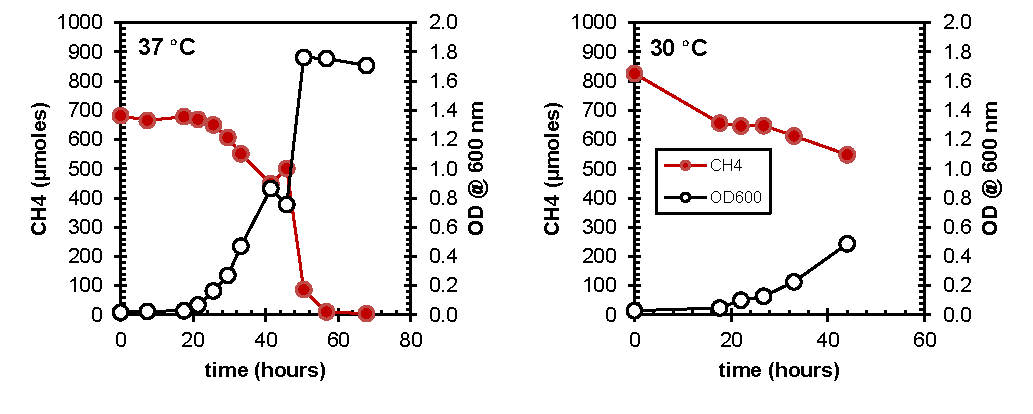
\includegraphics[width=0.95\textwidth]{figures/Fig4.S1}
	\caption[Preliminary growth curves of \emph{M. capsulatus} Bath]{Measured CH\textsubscript{4}
		concentrations and optical densities (OD) during preliminary experiments
		at 37~°C (left) and 30~°C (right) with starter cultures of \emph{M.}
		\emph{capsulatus} (Bath).}
	\label{fig:4:S1}
\end{figure*}

\emph{Methylococcus capsulatus} strain Bath cultures were grown in 10 ml
of nitrate mineral salts medium supplemented with 5~µM
CuSO\textsubscript{4} \parencite{Welander+Summons_2012_PNAS}. Serum bottles (160
cm\textsuperscript{3}) were inoculated with 2\%(v/v) inoculum from a
starter culture that had grown for ca.\ 30 hours, stoppered and sealed
without removing ambient air, and injected with 20 cm\textsuperscript{3}
SATP (\textasciitilde{}810~µmol) of methane from commercially-sourced
cylinders using a gas-tight syringe. Tests indicated that the starting
gas compositions were consistent within analytical error (±5\%) between
serum bottles. Multiple serum bottles were inoculated for each of the
two experimental temperatures (\autoref{tab:4:1}). Cultures were incubated at 30
or 37~°C while shaking at 225 rpm and sacrificed at given times by
adding 1 ml of 1 M hydrochloric acid. Each row in \autoref{tab:4:1} shows the
composition of one serum bottle at the time at which the experiment was
stopped. Experimental timepoints were selected based on monitoring of
growth during preliminary incubations of starter cultures (by tracking
optical density, see \autoref{fig:4:S1}). However, to minimize
puncturing of the serum bottles during the isotopic fractionation
experiments, optical densities were not measured for the samples
analyzed for isotopologues shown in \autoref{tab:4:1}. The combination of constant
agitation, a large headspace volume relative to liquid volume, and high
initial CH\textsubscript{4} partial pressures (\textgreater{}0.1 atm)
ensures that diffusion into the liquid from the headspace does not limit
the rate of methane consumption \parencite{Templeton++_2006_GCA,Nihous_2008_GCA}.

\subsection{Analytical techniques}\label{sec:4:analytical-techniques}

Concentrations of headspace gases, including CH\textsubscript{4} and
CO\textsubscript{2}, were determined via gas chromatography (GC) using a
Shimadzu GC-2014 gas chromatograph configured with a packed column
(Carboxen-1000, 5$'$ × 1/8$''$, Supelco, Bellefonte, Pennsylvania, USA) held
at 140~°C and argon carrier gas, and thermal conductivity and
methanizer-flame ionization detectors. Subsamples of the headspace (0.20
cm\textsuperscript{3} at laboratory temperature, \textasciitilde{}23~°C)
from each serum bottle were taken via a gas-tight syringe and injected
onto the column. Gas concentrations were determined directly as partial
pressures. Accuracy of the analyses, evaluated from standards, was ±5\%.
The fraction of initial methane remaining, \emph{f}, in each batch
culture was calculated from these measurements (\autoref{tab:4:1}), with
uncertainties propagated following \textcite{Ku_1969_JResNBS}.

Samples of methane were purified via cryofocusing--preparative gas
chromatography through a packed column (Carboxen-1000, 5$'$ × 1/8$''$,
Supelco) held at 30~°C with helium carrier gas, and cryotrapping of the
eluted methane on activated charcoal at liquid nitrogen temperature
\parencite{Wang++_2015_S}. The relative abundances of the methane stable
isotopologues \textsuperscript{12}CH\textsubscript{4},
\textsuperscript{13}CH\textsubscript{4},
\textsuperscript{12}CH\textsubscript{3}D, and
\textsuperscript{13}CH\textsubscript{3}D were measured using a tunable
infrared laser direct absorption spectroscopy technique described
previously \parencite{Ono++_2014_AC,Wang++_2015_S}.

Isotope values are reported herein using standard
delta-notation.\footnote{Definitions: δ\textsuperscript{13}C =
	(\textsuperscript{13}C/\textsuperscript{12}C)\textsubscript{sample}/(\textsuperscript{13}C/\textsuperscript{12}C)\textsubscript{PDB}
	$-$ 1, and δD = (D/H)\textsubscript{sample}/(D/H)\textsubscript{SMOW} $-$
	1 {[}for natural samples of methane, δ\textsuperscript{13}C~$\approx$~	(\textsuperscript{13}CH\textsubscript{4}/\textsuperscript{12}CH\textsubscript{4})\textsubscript{sample}/(\textsuperscript{13}CH\textsubscript{4}/\textsuperscript{12}CH\textsubscript{4})\textsubscript{PDB}
	$-$ 1 and δD $\approx$ ¼
	(\textsuperscript{12}CH\textsubscript{3}D/\textsuperscript{12}CH\textsubscript{4})\textsubscript{sample}/(D/H)\textsubscript{SMOW}
	$-$ 1{]}.} In accordance with IUPAC recommendations \parencite{Coplen_2011_RCM}, we
have omitted the factor of 1000‰ from the definition of δ and other
isotope values (including Δ\textsuperscript{13}CH\textsubscript{3}D,
below). Carbon and hydrogen isotope values were calibrated against
community reference materials NGS-1 and NGS-3 \parencite{Wang++_2015_S}.

The abundance of \textsuperscript{13}CH\textsubscript{3}D is tracked via
the Δ\textsuperscript{13}CH\textsubscript{3}D value, defined according
to \textcite{Ono++_2014_AC} as:
\begin{equation}\label{eqn:4:3}
\mathrm\Delta^{13}{\text{CH}}_3\text{D}=\ln Q\text{,\; where\ }Q=\frac{\bigl\lbrack{}^{13}{\text{CH}}_3\text{D}\bigr\rbrack\bigl\lbrack{}^{12}{\text{CH}}_4\bigr\rbrack}{\bigl\lbrack{}^{13}{\text{CH}}_4\bigr\rbrack\bigl\lbrack{}^{12}{\text{CH}}_3\text{D}\bigr\rbrack}
\end{equation}
Here, \emph{Q} is the reaction quotient for \mrefs[]{Reaction}{eqn:4:2}, and
Δ\textsuperscript{13}CH\textsubscript{3}D $ \approx $ \emph{Q} $-$ 1 because
\emph{Q} is close to unity in the natural and experimental systems
studied herein.\footnote{From the approximation
	\(\ln{\left( 1 + x \right) \approx x}\) for values of \emph{x} close
	to zero.} For a methane sample that has attained a distribution of
isotopes among all isotopologues consistent with equilibrium at a given
temperature, \emph{Q} = \emph{K}. The temperature dependence of the
equilibrium Δ\textsuperscript{13}CH\textsubscript{3}D value was
theoretically estimated and experimentally calibrated previously \parencite{Wang++_2015_S}.

Methane samples with a wide range of δD values ($-$480‰ to +500‰ vs.\ SMOW) were prepared and thermally-equilibrated over platinum catalyst at
300~°C to correct for the nonlinearity in the spectroscopic analysis
described by \textcite{Ono++_2014_AC}.

\subsection{Calculation of isotope and isotopologue fractionation
	factors}\label{sec:4:calculation-of-isotope-and-isotopologue-fractionation-factors}

The MMO-catalyzed reaction between methane and O\textsubscript{2} to
produce the intermediate product methanol is the first in a sequence of
enzymatic reactions involved in aerobic methanotrophy \parencite{Sirajuddin+Rosenzweig_2015_Bc}. We focus on this reaction because it is the most
important isotopically-fractionating step in this sequence as it is
considered to be both rate-limiting and isotope-sensitive \parencite{Nesheim+Lipscomb_1996_Bc} under the studied experimental conditions. Limitation of
the rate of methane consumption by this step requires that methane
diffusion into and out of the cells be rapid relative to MMO catalysis.
Following \textcite{Nihous_2010_IEHS}, we assume that isotopic fractionation
associated with transfer of methane across cell membranes is negligible.

The reaction scheme for the first step of the aerobic oxidation of the
methane isotopologues \textsuperscript{12}CH\textsubscript{4},
\textsuperscript{13}CH\textsubscript{4},
\textsuperscript{12}CH\textsubscript{3}D, and
\textsuperscript{13}CH\textsubscript{3}D can be described by the
following six chemical reactions:
\begin{align}
{}^{12}{\text{CH}}_4&\longrightarrow{}^{12}{\text{CH}}_3\text{OH} \label{eqn:4:4}\\
{}^{13}{\text{CH}}_4&\longrightarrow{}^{13}{\text{CH}}_3\text{OH} \label{eqn:4:5}\\
{}^{12}{\text{CH}}_3\text{D}&\longrightarrow{}^{12}{\text{CH}}_3\text{OH} \label{eqn:4:6}\\
{}^{12}{\text{CH}}_3\text{D}&\longrightarrow{}^{12}{\text{CH}}_2\text{DOH} \label{eqn:4:7}\\
{}^{13}{\text{CH}}_3\text{D}&\longrightarrow{}^{13}{\text{CH}}_3\text{OH} \label{eqn:4:8}\\
{}^{13}{\text{CH}}_3\text{D}&\longrightarrow{}^{13}{\text{CH}}_2\text{DOH} \label{eqn:4:9}
\end{align}

\subsubsection{Carbon isotope
	fractionation}\label{sec:4:carbon-isotope-fractionation}

Assuming that the reaction is irreversible, follows first-order
kinetics, and occurs in a closed system, the following differential
equations can be written for \textsuperscript{12}CH\textsubscript{4} and
\textsuperscript{13}CH\textsubscript{4}:
\begin{align}
\frac{d_{}^{\mathrm{12}}{\mathrm{C}\mathrm{H}_{\mathrm{4}}}}{{dt}} &= - k \cdot \bigl\lbrack{}_{}^{\mathrm{12}}{\mathrm{C}\mathrm{H}_{\mathrm{4}}} \bigr\rbrack \label{eqn:4:10} \\
\frac{d_{}^{\mathrm{13}}{\mathrm{C}\mathrm{H}_{\mathrm{4}}}}{{dt}} &= -_{}^{13}\alpha \cdot k \cdot \bigl\lbrack{}_{}^{\mathrm{13}}{\mathrm{C}\mathrm{H}_{\mathrm{4}}} \bigr\rbrack \label{eqn:4:11}
\end{align}
where \emph{k} is the rate constant for
\textsuperscript{12}CH\textsubscript{4} consumption (\mrefs[]{Reaction}{eqn:4:4}), and
\textsuperscript{13}$\alpha$ is the fractionation factor for
\textsuperscript{13}C/\textsuperscript{12}C (ratio of rate constants for
\mrefs[]{Reactions}{eqn:4:5} and \ref{eqn:4:4}).

Combining \mrefs[]{Eqns.}{eqn:4:10} and \ref{eqn:4:11}, eliminating \emph{dt}, and integrating from
\emph{f} = 1 (initial) to \emph{f} yields the equation:
\begin{equation}\label{eqn:4:12}
\ln\left( \frac{\bigl\lbrack{}_{}^{\mathrm{13}}{\mathrm{C}\mathrm{H}_{\mathrm{4}}} \bigr\rbrack_{f}}{\bigl\lbrack{}_{}^{\mathrm{13}}{\mathrm{C}\mathrm{H}_{\mathrm{4}}} \bigr\rbrack_{\mathrm{\text{init}}}} \right) = {}_{}^{13}\alpha \cdot \ln\left( \frac{\bigl\lbrack{}_{}^{\mathrm{12}}{\mathrm{C}\mathrm{H}_{\mathrm{4}}} \bigr\rbrack_{f}}{\bigl\lbrack{}_{}^{\mathrm{12}}{\mathrm{C}\mathrm{H}_{\mathrm{4}}} \bigr\rbrack_{\mathrm{\text{init}}}} \right)
\end{equation}

By subtracting
\(\ln\left( {\bigl\lbrack{}_{}^{\mathrm{12}}{\mathrm{C}\mathrm{H}_{\mathrm{4}}} \bigr\rbrack_{f}}\middle/{\bigl\lbrack{}_{}^{\mathrm{12}}{\mathrm{C}\mathrm{H}_{\mathrm{4}}} \bigr\rbrack_{\mathrm{\text{init}}}} \right)\)
from each side of \autoref{eqn:4:12}, and applying the approximations
\(f \approx \allowbreak \left.{\bigl\lbrack{}_{}^{\mathrm{12}}{\mathrm{C}\mathrm{H}_{\mathrm{4}}} \bigr\rbrack_{f}}\middle/{\bigl\lbrack{}_{}^{\mathrm{12}}{\mathrm{C}\mathrm{H}_{\mathrm{4}}} \bigr\rbrack_{\mathrm{\text{init}}}}\right.\)
and
{[}\textsuperscript{13}CH\textsubscript{4}{]}$\big/${[}\textsuperscript{12}CH\textsubscript{4}{]}
$ \approx $ {[}\textsuperscript{13}C{]}$\big/${[}\textsuperscript{12}C{]}, we obtain a form of the
classic ``Rayleigh equation'' \parencite{Mariotti++_1981}:
\begin{equation}\label{eqn:4:13}
\ln\frac{\mathrm{\updelta}^{13}\mathrm{C} + 1}{{\mathrm{\updelta}^{13}\mathrm{C}}_{\mathrm{\text{init}}} + 1} = \left({}_{}^{13}\alpha - 1 \right)\,\ln f
\end{equation}

\subsubsection{Hydrogen isotope
	fractionation}\label{sec:4:hydrogen-isotope-fractionation}

For the D-substituted isotopologue
\textsuperscript{12}CH\textsubscript{3}D, there are two ways to break a
carbon-hydrogen bond. These two pathways are described by \mrefs[]{Reactions}{eqn:4:6} and \ref{eqn:4:7}. The former involves the breakage of the C--D bond (accompanied by
a primary isotope effect, described by the fractionation factor
\textsuperscript{D}$\alpha$\textsubscript{p}), while the latter involves the
breakage of any of the three C--H bonds \emph{adjacent} to the C--D bond
(incurring a secondary isotope effect,
\textsuperscript{D}$\alpha$\textsubscript{s}). Thus, the overall rate of the
oxidation of \textsuperscript{12}CH\textsubscript{3}D to methanol can be
described by:
\begin{equation}\label{eqn:4:14} 
\frac{d_{}^{\mathrm{12}}{\mathrm{C}\mathrm{H}_{\mathrm{3}}\mathrm{D}}}{{dt}} = \textstyle - \frac{1}{4} \cdot{}_{}^{\mathrm{D}}\alpha_{\mathrm{p}} \cdot k \cdot \bigl\lbrack{}_{}^{\mathrm{12}}{\mathrm{C}\mathrm{H}_{\mathrm{3}}\mathrm{D}} \bigr\rbrack - \frac{3}{4} \cdot{}_{}^{\mathrm{D}}\alpha_{\mathrm{s}} \cdot k \cdot \bigl\lbrack{}_{}^{\mathrm{12}}{\mathrm{C}\mathrm{H}_{\mathrm{3}}\mathrm{D}} \bigr\rbrack
\end{equation}

By lumping together \textsuperscript{D}$\alpha$\textsubscript{p} and
\textsuperscript{D}$\alpha$\textsubscript{s}, the rate equation can be
simplified to:
\begin{equation}\label{eqn:4:15}
\frac{d_{}^{\mathrm{12}}{\mathrm{C}\mathrm{H}_{\mathrm{3}}\mathrm{D}}}{{dt}} = \textstyle -_{}^{\mathrm{D}}\alpha \cdot k \cdot \bigl\lbrack{}_{}^{\mathrm{12}}{\mathrm{C}\mathrm{H}_{\mathrm{3}}\mathrm{D}} \bigr\rbrack
\end{equation}
where
\(_{}^{\mathrm{D}}\alpha = \frac{1}{4}{}_{}^{\mathrm{D}}\alpha_{\mathrm{p}} + \frac{3}{4}{}_{}^{\mathrm{D}}\alpha_{\mathrm{s}}\).

This parameterization of D/H fractionation is attractive in that it
allows for apparent overall isotopic fractionation factors to be
constrained by cell culture experiments and measurement with
conventional geochemical techniques (e.g., isotope ratio mass
spectrometry), without measurement of the individual reaction products.
Applying the same logic used in \autoref{sec:4:carbon-isotope-fractionation}, the following expression is
obtained:
\begin{equation}\label{eqn:4:16}
\ln\frac{\mathrm{\text{δD}} + 1}{\mathrm{\text{δD}}_{\mathrm{\text{init}}} + 1} = \left(_{}^{\mathrm{D}}\alpha - 1 \right)\,\ln f
\end{equation}

Combining \mrefs{Eqns.}{eqn:4:13} and~\ref{eqn:4:16} yields an equation describing the correlation
between carbon and hydrogen isotope fractionation:

\begin{equation}\label{eqn:4:17}
\ln\frac{\mathrm{\text{δD}} + 1}{\mathrm{\text{δD}}_{\mathrm{\text{init}}} + 1} = \left( \frac{{}_{}^{\mathrm{D}}\alpha - 1}{{}_{}^{13}\alpha - 1} \right)\ln\frac{\mathrm{\updelta}^{13}\mathrm{C} + 1}{{\mathrm{\updelta}^{13}\mathrm{C}}_{\mathrm{\text{init}}} + 1}
\end{equation}

\subsubsection{\texorpdfstring{\textsuperscript{13}CH\textsubscript{3}D
		fractionation}{13CH3D fractionation}}\label{sec:4:13ch3d-fractionation}

The rate of oxidation of \textsuperscript{13}CH\textsubscript{3}D can be
described by:
\begin{equation}\label{eqn:4:18}
\frac{d_{}^{\mathrm{13}}{\mathrm{C}\mathrm{H}_{\mathrm{3}}\mathrm{D}}}{{dt}} = \textstyle - \frac{1}{4} \cdot \gamma_{\mathrm{p}} \cdot{}_{}^{13}\alpha \cdot{}_{}^{\mathrm{D}}\alpha_{\mathrm{p}} \cdot k \cdot \bigl\lbrack{}_{}^{\mathrm{13}}{\mathrm{C}\mathrm{H}_{\mathrm{3}}\mathrm{D}} \bigr\rbrack - \frac{3}{4} \cdot \gamma_{\mathrm{s}} \cdot{}_{}^{13}\alpha \cdot{}_{}^{\mathrm{D}}\alpha_{\mathrm{s}} \cdot k \cdot \bigl\lbrack{}_{}^{\mathrm{13}}{\mathrm{C}\mathrm{H}_{\mathrm{3}}\mathrm{D}} \bigr\rbrack
\end{equation}

Here, we have introduced the terms $\gamma$\textsubscript{p} and
$\gamma$\textsubscript{s} to characterize deviations of the clumped
isotopologue fractionation factor from the product of the
\textsuperscript{13}C/\textsuperscript{12}C and D/H fractionation
factors ($\alpha$ values). When there is no deviation from this product (i.e.,
primary and secondary isotope fractionation factors for bond breakage in
\textsuperscript{13}CH\textsubscript{3}D follow what is referred to
hereafter as the ``product rule''), both $\gamma$\textsubscript{p} and
$\gamma$\textsubscript{s} are unity. Deviations from the product rule represent
a ``clumped isotopologue effect'' on bond breakage that arises from the
substitution of both \textsuperscript{13}C and D in the substrate
methane. To simplify the treatment of clumped isotopologue effects in
the absence of literature data for $\gamma$\textsubscript{p} and
$\gamma$\textsubscript{s}, we adopt the following form of the rate equation:
\begin{equation}\label{eqn:4:19}
\frac{d_{}^{\mathrm{13}}{\mathrm{C}\mathrm{H}_{\mathrm{3}}\mathrm{D}}}{{dt}} = - \gamma \cdot{}_{}^{13}\alpha \cdot{}_{}^{\mathrm{D}}\alpha \cdot k \cdot \bigl\lbrack{}_{}^{\mathrm{13}}{\mathrm{C}\mathrm{H}_{\mathrm{3}}\mathrm{D}} \bigr\rbrack
\end{equation}

Here, the ``gamma-factor'' ($\gamma$) is an empirically-constrained term that
describes an \emph{effective} clumped isotopologue fractionation factor.
Implicit in the use of \autoref{eqn:4:19} is that
\(\gamma \cdot{}_{}^{\mathrm{D}}\alpha = \frac{1}{4} \cdot \gamma_{\mathrm{p}} \cdot{}_{}^{\mathrm{D}}\alpha_{\mathrm{p}} + \frac{3}{4} \cdot \gamma_{\mathrm{s}} \cdot{}_{}^{\mathrm{D}}\alpha_{\mathrm{s}}\)
(from the definition of \textsuperscript{D}$\alpha$ in \autoref{sec:4:hydrogen-isotope-fractionation}; also see
discussion in \autoref{sec:4:fractionation-of-13ch3d}). This condition is satisfied, although not
uniquely, when $\gamma$ is equal to both $\gamma$\textsubscript{p} and
$\gamma$\textsubscript{s}.

\mrefs[]{Equation}{eqn:4:19} is convenient because it allows for $\gamma$ to be constrained by
measurements of the methane isotopologues in experiments conducted at
natural abundance without the use of isotopically labeled substrates or
measurement of individual isotopically-substituted products. Integration
of \autoref{eqn:4:19} combined with \autoref{eqn:4:10}, subtraction of the isotopologue-ratio
forms of \mrefs[]{Eqns.}{eqn:4:13} and \autoref{eqn:4:16} from the result, and substitution of the
definition of Δ\textsuperscript{13}CH\textsubscript{3}D (\autoref{eqn:4:3}) yields:
\begin{equation}\label{eqn:4:20}
\Delta_{}^{\mathrm{13}}{\mathrm{C}\mathrm{H}_{\mathrm{3}}\mathrm{D}} = {\Delta_{}^{\mathrm{13}}{\mathrm{C}\mathrm{H}_{\mathrm{3}}\mathrm{D}}}_{\mathrm{\text{initial}}} + \left( \gamma \cdot{}_{}^{13}\alpha \cdot{}_{}^{\mathrm{D}}\alpha -{}_{}^{13}\alpha -{}_{}^{\mathrm{D}}\alpha + 1 \right) \cdot \ln f\
\end{equation}

Adopting this greatly simplified treatment necessarily means that
differences in primary and secondary isotope effects for different forms
of the enzyme in different methanotroph species are masked and lumped
into an ``effective'' fractionation factor. A similar line of reasoning
was used by \textcite{Stolper++_2015_GCA} to simplify the representation of a
model methanogenic system.

\section{Results }\label{sec:4:results}


\begin{SCfigure}
	\centering
	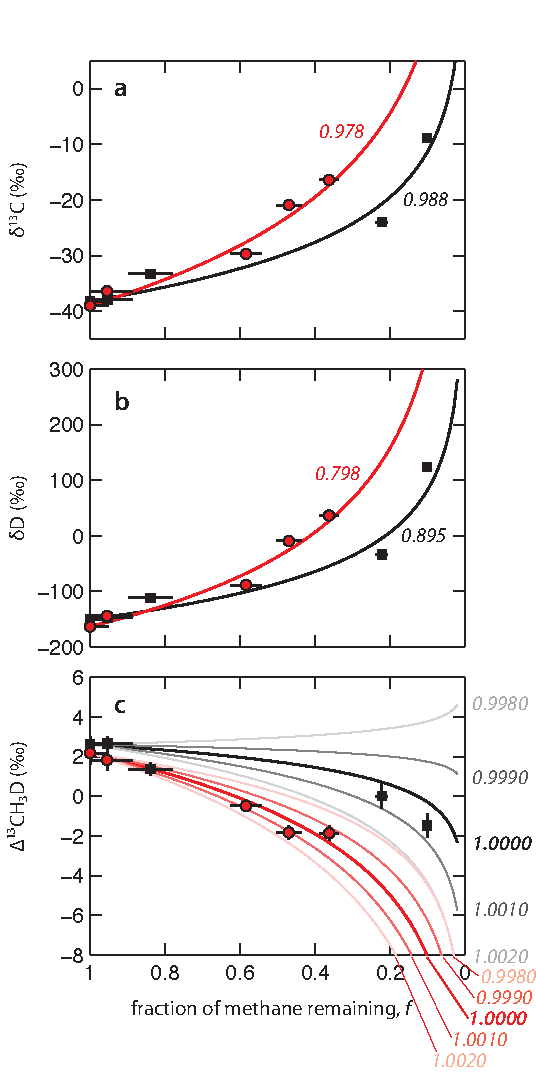
\includegraphics[width=0.5\textwidth]{figures/Fig4.1}
	\caption[Measured and modeled δ\textsuperscript{13}C, δD, and Δ\textsuperscript{13}CH\textsubscript{3}D values in batch cultures]{Measured and modeled changes in \textbf{(a)}
		δ\textsuperscript{13}C, \textbf{(b)} δD, and \textbf{(c)}
		Δ\textsuperscript{13}CH\textsubscript{3}D of residual methane as a
		function of \emph{f}, the fraction of initial methane remaining. Data
		points from the 30 and 37~°C experiments (\autoref{tab:4:1}) are shown with black
		and red symbols, respectively. Horizontal error bars represent
		propagated ±1$\sigma$ uncertainties from GC measurements, and vertical error
		bars represent 95\% confidence intervals from isotopologue ratio
		analyses. Solid lines represent the modeled values (from \mrefs[]{Eqns.}{eqn:4:13}, \ref{eqn:4:16},
		and \ref{eqn:4:20}) based on the calculated weighted-average carbon- and
		hydrogen-isotope fractionation factors for each set of experiments as
		listed in \autoref{tab:4:1}. Labels in \emph{italics} represent
		\textsuperscript{13}$\alpha$, \textsuperscript{D}$\alpha$, \& $\gamma$, respectively, in
		panels (a), (b), \& (c). Panel (c) shows model results calculated
		assuming different values of $\gamma$ varying between 0.9980 and 1.0020.}
	\label{fig:4:1}
\end{SCfigure}


\begin{sidewaystable}\centering
	\begin{threeparttable}
		\caption[Experimental results and calculated fractionation
		factors for batch cultures of \emph{M.\ capsulatus}]{Experimental results and calculated fractionation
		factors for batch cultures of \emph{Methylococcus capsulatus} Bath.
		Uncertainties (±1$\sigma$) listed for \emph{f}, \textsuperscript{13}$\alpha$,
		\textsuperscript{D}$\alpha$, and $\gamma$ are propagated from those associated with
		individual measurements according to standard formulas \parencite{Ku_1969_JResNBS}.}
		\label{tab:4:1}
		\begin{tabular}{lc r@{\;}c@{\;}l r r r r@{\;}c@{\;}l r@{\;}c@{\;}l r@{\;}c@{\;}l r@{\;}c@{\;}l}
			\toprule
			& time (h) & \multicolumn{3}{c}{\emph{f}} & CO\textsubscript{2}
			(cm\textsuperscript{3})\tnote{a} & δ\textsuperscript{13}C
			(‰)\tnote{c} & δD (‰)\tnote{c} & \multicolumn{3}{c}{
			Δ\textsuperscript{13}CH\textsubscript{3}D (‰)\tnote{c} } &
			\multicolumn{3}{c}{ \textsuperscript{13}$\alpha$ } & \multicolumn{3}{c}{ \textsuperscript{D}$\alpha$ } & \multicolumn{3}{c}{ $\gamma$ }\tabularnewline
			\midrule
			& & & & & & & & & & & & & & & & & & &\tabularnewline
			\emph{30~°C} & 0 & 1.00 & ± & 0.05\tnote{b} & \textless{}0.2 &
			$-$38.27 & $-$150.12 & 2.61 & ± & 0.43 & & & & & & & & &\tabularnewline
			& 12 & 0.95 & ± & 0.07 & 0.6 & $-$37.94 & $-$147.20 & 2.66 & ± & 0.34 &
			0.993 & ± & 0.011 & 0.928 & ± & 0.107 & 0.9983 & ± &
			0.0130\tabularnewline
			& 36 & 0.84 & ± & 0.06 & 1.9 & $-$33.31 & $-$111.79 & 1.36 & ± & 0.34 &
			0.971 & ± & 0.012 & 0.749 & ± & 0.101 & 0.9997 & ± &
			0.0060\tabularnewline
			& --\tnote{d} & 0.22 & ± & 0.02 & 10.3 & $-$24.00 & $-$33.36 &
			$-$0.01 & ± & 0.60 & 0.990 & ± & 0.0005 & 0.915 & ± & 0.004 & 1.0010 & ± &
			0.0005\tabularnewline
			& 60 & 0.10 & ± & 0.01 & 9.8 & $-$8.81 & 123.90 & $-$1.48 & ± & 0.60 & 0.987
			& ± & 0.0004 & 0.878 & ± & 0.004 & 1.0002 & ± & 0.0004\tabularnewline \cmidrule{12-20} 
			& & & & & & & \multicolumn{4}{r}{weighted average\tnote{e}} & 0.988 & ± & 0.0003 &
			0.895 & ± & 0.003 & 1.0005 & ± & 0.0003\tabularnewline
			& & & & & & & & & & & & & & & & & & &\tabularnewline
			\emph{37~°C} & 0 & 1.00 & ± & 0.05\tnote{b} & n.d. & $-$39.06 &
			$-$163.57 & 2.17 & ± & 0.59 & & & & & & & & &\tabularnewline
			& 41 & 0.95 & ± & 0.07 & n.d. & $-$36.45 & $-$144.23 & 1.82 & ± & 0.53 &
			0.943 & ± & 0.086 & 0.516 & ± & 0.726 & 0.9585 & ± &
			0.2130\tabularnewline
			& 44 & 0.58 & ± & 0.04 & 2.5 & $-$29.68 & $-$88.51 & $-$0.48 & ± & 0.30 &
			0.982 & ± & 0.002 & 0.840 & ± & 0.021 & 1.0025 & ± &
			0.0015\tabularnewline
			& 48 & 0.47 & ± & 0.03 & 4.8 & $-$20.95 & $-$9.20 & $-$1.82 & ± & 0.36 & 0.975
			& ± & 0.002 & 0.776 & ± & 0.021 & 0.9997 & ± & 0.0014\tabularnewline
			& 51 & 0.36 & ± & 0.03 & 6.3 & $-$16.39 & 36.83 & $-$1.87 & ± & 0.38 & 0.977
			& ± & 0.002 & 0.788 & ± & 0.015 & 0.9989 & ± & 0.0011\tabularnewline \cmidrule{12-20} 
			& & & & & & & \multicolumn{4}{r}{weighted average\tnote{e}} & 0.978 & ± & 0.001 &
			0.798 & ± & 0.010 & 1.0000 & ± & 0.0007\tabularnewline
			& & & & & & & & & & & & & & & & & & &\tabularnewline
			\bottomrule
		\end{tabular}
		{\small n.d., not determined}
		\begin{tablenotes}
				\item[a] Total inorganic carbon in the bottle (including
				gaseous CO\textsubscript{2} and dissolved inorganic carbon), reported as
				cm\textsuperscript{3}-equivalent of CO\textsubscript{2} at standard
				ambient temperature and pressure (SATP; 25~°C, 1 bar), was estimated
				from headspace CO\textsubscript{2} concentration (determined via GC),
				the Henry's law constant for CO\textsubscript{2} at room temperature,
				and the volume of headspace and of HCl-spiked medium. Uncertainty is
				estimated at ±10\%. Quantitative conversion of initial
				CH\textsubscript{4} (see \autoref{sec:4:cultures}) into CO\textsubscript{2} (i.e., 100\%
				oxidation with no incorporation of CH\textsubscript{4}-derived carbon
				into biomass) would yield 20~cm\textsuperscript{3} SATP of
				CO\textsubscript{2}.
				
				\item[b] An uncertainty of ±5\% was assigned to the initial
				value of \emph{f} to account for variability in starting amounts of
				methane between bottles (see \autoref{sec:4:cultures}). This uncertainty is propagated
				throughout the calculations for later timepoints.
				
				\item[c] Values for δ\textsuperscript{13}C, δD, and
				Δ\textsuperscript{13}CH\textsubscript{3}D are reported relative to PDB,
				SMOW, and the stochastic distribution, respectively. Uncertainties for
				δ\textsuperscript{13}C, δD (both ca.\ 0.1‰), and
				Δ\textsuperscript{13}CH\textsubscript{3}D (listed) are 95\% confidence
				intervals over all cycles in a single analysis \parencite[e.g.,][]{Wang++_2015_S},
				but are conservatively treated as 1$\sigma$ for purposes of error propagation.
				
				\item[d] Time not recorded.
				
				\item[e] Weighted means of each set of \textsuperscript{13}$\alpha$,
				\textsuperscript{D}$\alpha$, and $\gamma$ values, weighted by 1/$\sigma$\textsuperscript{2}.
				Uncertainty (1$\sigma$) in weighted means was estimated following \textcite{Bevington+Robinson_3e}.
		\end{tablenotes}
	\end{threeparttable}
\end{sidewaystable}


During the course of the experiments at 30 and 37~°C, the concentration
of methane in the headspace decreased and the concentration of
CO\textsubscript{2} increased (\autoref{tab:4:1}). The bottles incubated at 37~°C
exhibited a lag phase (observed in preliminary experiments with starter
cultures, \autoref{fig:4:S1}), with a rapid transition into active
methane consumption around 41 hours after inoculation (\autoref{tab:4:1}), whereas
in the 30~°C experiments, methane consumption began immediately after
inoculation, but at an apparently lower rate. Based on mass balance of
measured CO\textsubscript{2} and CH\textsubscript{4} concentrations
relative to initial CH\textsubscript{4} (\autoref{tab:4:1}), \textasciitilde{}7\%
to 41\% of carbon was not accounted for; this fraction of carbon was
likely incorporated into cellular biomass (\emph{b} in \autoref{eqn:4:1}). This
range of \emph{b} values is similar to ranges observed in previous
studies \parencite[e.g., 0.1$-$0.5 in][]{Templeton++_2006_GCA}.

The initial isotopic composition of the methane used was different
between the two sets of experiments (\autoref{tab:4:1}). As methane was consumed,
the δ\textsuperscript{13}C and δD values of the residual methane
increased (\autoref{fig:4:1}), indicating a preferential consumption of the lighter
\textsuperscript{12}C and \textsuperscript{1}H by the bacteria.
Conversely, Δ\textsuperscript{13}CH\textsubscript{3}D values of the
residual methane decreased as methane was consumed, starting from
initial values of ca.\ +2.6‰ and +2.2‰, and decreasing to ``anticlumped''
(\textless{}0‰) values of ca.\ $-$1.5‰ and $-$1.9‰, respectively, at the last
time points sampled in the 30 and 37~°C experiments (\autoref{tab:4:1}).

Using \mrefs{Eqns.}{eqn:4:13}, \ref{eqn:4:16}, and \ref{eqn:4:20}, values of the fractionation factors
\textsuperscript{13}$\alpha$, \textsuperscript{D}$\alpha$, and $\gamma$ were calculated for
each time point after the initial (\autoref{tab:4:1}). All calculations used the
initial timepoint as the reference starting point; thus, the
fractionation factors reported are averaged over the entire reaction
occurring in the bottle, and contain correlated errors linked to the
uncertainty in data from the initial timepoint. Fractionation factors
were calculated for each timepoint, rather than over all bottles in an
experiment, to avoid artifacts from variable growth between bottles,
particularly at the lower temperature of 30~°C (see \autoref{fig:4:S1}). In the earlier time points, the error in the calculated
fractionation factors is large because of uncertainties in \emph{f} and
in Δ\textsuperscript{13}CH\textsubscript{3}D. For each set of
experiments, the weighted-averages of the fractionation factors were
determined, and are listed in \autoref{tab:4:1}, and the corresponding
trajectories (using experimental \textsuperscript{13}$\alpha$ and
\textsuperscript{D}$\alpha$ values, and variable $\gamma$) are depicted in \autoref{fig:4:1}.

Isotopic fractionation of D/H was substantially greater in magnitude
than that of \textsuperscript{13}C/\textsuperscript{12}C (\mrefs[a]{Fig.}{fig:4:2}). In
general, a greater degree of both carbon- and hydrogen-isotope
fractionation was observed in the bottles incubated at 37~°C than at 30
°C (\mrefs[b]{Fig.}{fig:4:2}). No systematic changes in the magnitude of isotope
fractionation were observed over the course of the experiments (\autoref{tab:4:1}). A similar, tight correlation of D/H and
\textsuperscript{13}C/\textsuperscript{12}C fractionation is observed
between the two sets of experiments (\mrefs[a]{Fig.}{fig:4:2}).

Calculated $\gamma$ values for each experimental timepoint are shown in \autoref{tab:4:1}. All values were close to unity, and showed no systematic changes over
the course of incubation. The weighted-average $\gamma$ values for the
experiments were identical to unity within 2$\sigma$ error (1.0005 ± 0.0006 and
1.0000 ± 0.0014 for the 30 and 37~°C experiments, respectively).

\section{Discussion}\label{sec:4:discussion}

\subsection{Isotope and isotopologue fractionation during aerobic
	methanotrophy}\label{sec:4:isotope-and-isotopologue-fractionation-during-aerobic-methanotrophy}

\subsubsection{\texorpdfstring{Fractionation of methane
		\textsuperscript{13}C/\textsuperscript{12}C and D/H
		ratios}{Fractionation of methane 13C/12C and D/H ratios}}\label{sec:4:fractionation-of-methane-13c12c-and-dh-ratios}

A wide range of carbon isotope fractionation factors
{[}\textsuperscript{13}$\varepsilon$ (= \textsuperscript{13}$\alpha$ $-$ 1) ranging from $-$38‰
to $-$3‰{]} have been reported in culture- and field-based studies \parencite[see][and references therein]{Templeton++_2006_GCA}. The variable nature
of the magnitude of observed carbon isotope effects complicates
application of measurements of individual carbon isotope ratios in
diagnosing the presence and extent of methanotrophy in the environment.
As such, the use of paired δ\textsuperscript{13}C and δD data has been
suggested as a possible method of removing some levels of ambiguity
associated with the sole use of carbon isotopes \parencite{Elsner++_2005_EST}.
Although the absolute magnitudes of isotope fractionation may vary due
to ``masking effects'' from preceding isotopically-insensitive steps
such as transport across membranes or binding to an enzyme \parencite{Feisthauer++_2011_GCA}, a correlation between the fractionation of the carbon and
hydrogen isotopes can be expected because both are principally
influenced by the breakage of the C--H bond. Such a correlation was
first noted by \textcite{Coleman++_1981_GCA}, with later studies by \textcite{Kinnaman++_2007_GCA,Powelson++_2007_EST,Feisthauer++_2011_GCA} corroborating
the observations in pure culture and in enrichments from other
environments. The published values of
\textsuperscript{D}$\varepsilon$/\textsuperscript{13}$\varepsilon$, corresponding to the slope
of the gray lines in \mrefs[a]{Fig.}{fig:4:2}, range from 5.9 to 14.9, with a mean of 8.9
± 2.3 {[}standard deviation (1$\sigma$), \emph{n} = 15{]}. The best-fit value
of \textsuperscript{D}$\varepsilon$/\textsuperscript{13}$\varepsilon$ for the data shown in
\autoref{tab:4:1} is 9.14, a value which appears independent of the two growth
temperatures tested, and which falls near the middle of the published
range.


\begin{figure*}
	\centering
	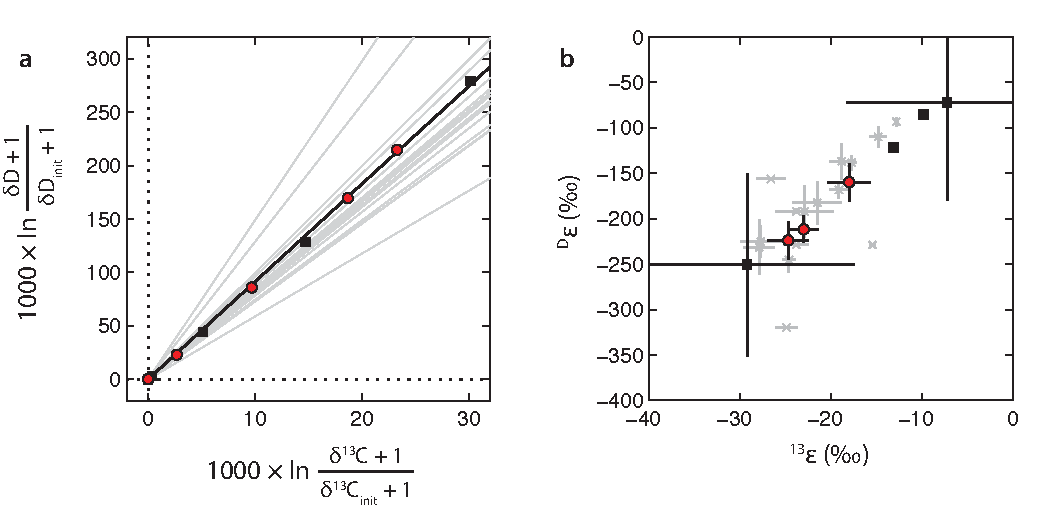
\includegraphics[width=0.95\textwidth]{figures/Fig4.2}
	\caption[\textsuperscript{13}C/\textsuperscript{12}C and D/H fractionation by aerobic methanotrophs]{Relationship between fractionation of carbon and
		hydrogen isotopes. \textbf{(a)} Data from the 30 and 37~°C experiments (\autoref{tab:4:1})
		are shown with black and red symbols, respectively. Black line (\emph{y}
		= 9.14 \emph{x}) represents the best-fit regression through the data.
		From \autoref{eqn:4:17}, the slope of this line is (\textsuperscript{D}$\alpha$ $-$
		1)/(\textsuperscript{13}$\alpha$ $-$ 1), or
		\textsuperscript{D}$\varepsilon$/\textsuperscript{13}$\varepsilon$. Near the origin, the
		\emph{x}- and \emph{y}-axes are approximately equal to
		δ\textsuperscript{13}C $-$ δ\textsuperscript{13}C\textsubscript{init} and
		δD $-$ δD\textsubscript{init}, respectively; this approximation becomes
		less accurate with increasing distance from the origin, particularly for
		hydrogen \parencite{Sessions+Hayes_2005_GCA}. Gray lines represent
		previously-reported correlations between fractionation of carbon and
		hydrogen isotopes by aerobic methanotrophs determined from experiments
		with pure cultures \parencite{Feisthauer++_2011_GCA} and enrichment cultures
		\parencite{Coleman++_1981_GCA,Kinnaman++_2007_GCA,Powelson++_2007_EST}.
		\textbf{(b)} Fractionation factors ($\varepsilon$, defined as $\alpha$ $-$ 1) calculated for
		individual bottle incubations from this study (\autoref{tab:4:1}) plotted against
		fractionation factors reported in the cited studies (gray). One point
		from the 37~°C experiment (41 h) was not plotted because of large
		uncertainties arising from a minimal extent of reaction.}
	\label{fig:4:2}
\end{figure*}


The consistency of the determined
\textsuperscript{D}$\varepsilon$/\textsuperscript{13}$\varepsilon$ ratios with those in the
literature provides confidence that results regarding the behavior of
Δ\textsuperscript{13}CH\textsubscript{3}D (discussed below) during
aerobic methane oxidation by \emph{M.~capsulatus} (Bath) can be
generalizable to other strains grown under other conditions. Further
experiments with these strains grown under different conditions to
examine clumped isotopologue fractionation will help to determine if
this hypothesis is valid. In a previous study, various strains of
bacteria \parencite[including \emph{M.~capsulatus}, which has two pMMOs and one
sMMO;][]{Ward++_2004_PLOSBiol} grown in batch cultures under different
copper (Cu) concentrations (with pMMO expressed under Cu-rich conditions
and sMMO under low Cu) demonstrated consistently correlated
fractionations of carbon and hydrogen isotopes, without apparent
correlation to physiology or growth condition \parencite{Feisthauer++_2011_GCA}.
Values of \textsuperscript{D}$\varepsilon$/\textsuperscript{13}$\varepsilon$ derived from that
study range from 7.3 to 8.8, and are close to the average
\textsuperscript{D}$\varepsilon$/\textsuperscript{13}$\varepsilon$ ratio from our dataset (9.14, \mrefs[a]{Fig.}{fig:4:2}). In particular, \emph{M.~cap\-su\-la\-tus} grown at 45~°C induced
isotopic fractionations of \textsuperscript{13}$\alpha$ = 0.972 ± 0.002 and
\textsuperscript{D}$\alpha$ = 0.769 ± 0.030 (published uncertainties were
listed as 95\% confidence interval, approximately 2$\sigma$) under Cu-rich
conditions, and under Cu-poor conditions, similar values of
\textsuperscript{13}$\alpha$ = 0.977 ± 0.003 and \textsuperscript{D}$\alpha$ = 0.808 ±
0.029 \parencite{Feisthauer++_2011_GCA}. The corresponding
\textsuperscript{D}$\varepsilon$/\textsuperscript{13}$\varepsilon$ ratios (with propagated
\textasciitilde{}2$\sigma$ uncertainties) indicated by their data are 8.3 ± 1.1
and 8.4 ± 1.7 under Cu-rich and Cu-poor conditions, respectively. These
values are indistinguishable from the
\textsuperscript{D}$\varepsilon$/\textsuperscript{13}$\varepsilon$ ratio derived from regression
through our experimental data (9.14 ± 0.14, 2$\sigma$; see \autoref{tab:4:2}). This
correspondence of \textsuperscript{D}$\varepsilon$/\textsuperscript{13}$\varepsilon$ ratios
suggests that the proposed product rule for $\gamma$ values (see \autoref{sec:4:fractionation-of-13ch3d})
could be valid for \emph{M. capsulatus} expressing either pMMO or sMMO,
and may hold for many other methanotrophic strains cultured under
various conditions.

Insights into the origin of D/H fractionation during methane oxidation
have been obtained from studies which separately constrain the primary
and secondary hydrogen isotope effects. Using molecular dynamics
simulations, \textcite{Pudzianowski+Loew_1983_JPC} calculated the isotope effects
associated with the abstraction of H or D from CH\textsubscript{4} or
CH\textsubscript{3}D by atomic oxygen, O(\textsuperscript{3}P), as an
analog for the methane monooxygenase reaction. Their results, expressed
as fractionation factors, are \textsuperscript{D}$\alpha$\textsubscript{p} =
0.0296 and \textsuperscript{D}$\alpha$\textsubscript{s} = 0.763 (or 0.0179 and
0.759 when tunneling corrections were applied). Thus, the overall
isotope fractionation, \textsuperscript{D}$\alpha$ (see \autoref{eqn:4:15}), would be
0.580. This fractionation factor reflects a much larger magnitude of D/H
fractionation than is observed in either our experiments
(\textsuperscript{D}$\alpha$ as low as 0.718) or those reported in other
studies (plotted in \mrefs[b]{Fig.}{fig:4:2}). \textcite{Pudzianowski+Loew_1983_JPC} note,
however, that the transition state of the
CH\textsubscript{4}/CH\textsubscript{3}D + O(\textsuperscript{3}P)
reaction they modeled has only qualitative similarity to the transition
state of the methane hydrogen abstraction/hydroxylation reaction
performed by methane monooxygenase. Such fundamental differences between
the two processes may explain the difference between their calculated
fractionation and the experimental observations.

Multiple experimental determinations of the kinetic isotope effects for
H or D abstraction have been reported \parencite[e.g.,][and references therein]{Green+Dalton_1989_JBC,Rataj++_1991_JBC,Wilkins++_1994_EJB}. Values for the primary isotope effect (corresponding to
\textsuperscript{D}$\alpha$\textsubscript{p} = 0.73) and secondary isotope
effect (\textsuperscript{D}$\alpha$\textsubscript{s} = 0.93) have been reported
for methane oxidation by sMMO \parencite{Wilkins++_1994_EJB}. The overall
\textsuperscript{D}$\alpha$ calculated from these values (0.88 via \autoref{eqn:4:15}) is
not low enough to explain the observed D/H fractionations in culture
(\mrefs[b]{Fig.}{fig:4:2}). More recently, in experiments with a series of
multiply-deuterated isotopologues of methane, \textcite{Nesheim+Lipscomb_1996_Bc} determined that the isotopically-selective reaction of compound Q
(the key intermediate that oxidizes CH\textsubscript{4}) of the MMO
hydroxylase (MMOH\textsubscript{Q}) has very large primary and much
smaller secondary kinetic isotope effects corresponding to
\textsuperscript{D}$\alpha$\textsubscript{p} = 0.01--0.02 and
\textsuperscript{D}$\alpha$\textsubscript{s} = 0.9--1.0. Via \autoref{eqn:4:15}, the
corresponding overall hydrogen isotope fractionation,
\textsuperscript{D}$\alpha$, is then between \textasciitilde{}0.68 and
\textasciitilde{}0.76, a range which overlaps with the largest D/H
fractionation observed in our experiments (0.718, \autoref{tab:4:1}). Note that
such a direct quantitative comparison between isotope effects determined
from pure cultures and those from \emph{in vitro} experiments with
labeled substrates may not be meaningful, as in culture experiments the
fractionation induced by MMO is not necessarily the only factor
determining isotopic fractionation. Regardless, the very large primary
kinetic isotope effect implies that nearly all of the
\textsuperscript{12}CH\textsubscript{3}D reacts via the abstraction of
H, with only a minor fraction reacting via the abstraction of D. This
inference has potential implications for the interpretation of $\gamma$ factors
constrained by clumped isotopologue measurements (see \autoref{sec:4:fractionation-of-13ch3d}).

Generally larger bulk carbon and hydrogen isotopic fractionations were
observed in the 37~°C cultures, compared to those grown at 30~°C (\autoref{tab:4:1}). This trend is an apparent reversal of the normally-expected decrease
of kinetic isotope effects with increasing temperature. Such an inverse
temperature effect was previously observed by \textcite{Coleman++_1981_GCA} on
enrichment cultures grown at 11.5 and 26~°C. They excluded species
differences as the source of the apparent trend, and speculated that the
partial and differential expression of a combination of kinetic and
equilibrium isotope effects could explain their results.

In our experiments, only one strain of bacterium was cultured, thus also
excluding species differences as a reason for the observed inverse
temperature trend. If some D/H exchange with cellular water occurs
during C--H bond breakage and re-forming, the overall
\textsuperscript{D}$\varepsilon$ fractionation factor should be of smaller magnitude
than would otherwise be expected given the observed
\textsuperscript{13}$\varepsilon$ value (as the carbon does not exchange). {[}The δD
of water used in the cultures was not measured, but is estimated to be
between $-$95‰ and $-$32‰ based on tap water data from \textcite{Bowen++_2007_WRR}.
Based on the calibration of \textcite{Horibe+Craig_1995_GCA},\footnote{Comparisons
	of the fractionation factor for D/H equilibrium between
	CH\textsubscript{4}(\emph{g}) and H\textsubscript{2}O(\emph{l})
	derived from the calibrations of different studies reveal a
	substantial range in estimates \parencite[up to 30‰ at 30--37~°C, see][]{Wang++_2015_S}. This is mainly due to uncertainty in extrapolations of
	experimental calibrations of
	H\textsubscript{2}(\emph{g})/H\textsubscript{2}O(\emph{g}) at
	\textgreater{}200~°C to lower temperatures. However, this level of
	uncertainty does not impact the interpretation developed here.}
methane at D/H equilibrium with water at 30--37~°C would be expected to
have δD \textless{} $-$200‰, which is lower than the initial δD of methane
in both sets of experiments.{]} The observation that the ratio
\textsuperscript{D}$\varepsilon$/\textsuperscript{13}$\varepsilon$ is nearly identical between
the two temperatures (\mrefs[a]{Fig.}{fig:4:2}) therefore argues against C--H bond
re-equilibration as an explanation for smaller magnitudes of isotopic
fractionation in the 30~°C experiments. Furthermore, our additional
measurements of Δ\textsuperscript{13}CH\textsubscript{3}D indicate that
$\gamma$ values are indistinguishable (within 2$\sigma$, \autoref{tab:4:1}) between the two
experiments, lending additional support to the conclusion that kinetic
isotope fractionation dominates the observed isotope and isotopologue
signals.

Given the above analysis, an alternate explanation must be sought to
explain the observed apparent inverse temperature trend. According to
the theory of kinetic isotope fractionation \parencite[e.g.,][]{Bigeleisen_1949_JCP},
predictions of decreasing kinetic isotope effects with increasing
temperature are generally valid only for elementary reactions. The
aerobic oxidation of methane by \emph{M. capsulatus} consists of
multiple enzymatic steps, and thus expression of intrinsic kinetic
isotope effects may not be complete if the isotopically-sensitive
methane monooxygenase reaction is not fully rate-limiting. In
particular, models proposed to explain previously published experimental
data point to the depletion of soluble methane concentrations below
threshold levels required to maintain rates of mass transfer into the
cell as a control on the degree to which kinetic isotope effects are
expressed in culture \parencite{Nihous_2008_GCA,Nihous_2010_IEHS,Vavilin++_2015_IEHS}.
This behavior is analogous to that observed for
\textsuperscript{34}S/\textsuperscript{32}S ratios during microbial
sulfate reduction, where under low sulfate conditions, sulfur isotope
fractionation is suppressed due to rate limitation by the
isotopically-insensitive initial transport of sulfate into the cell
\parencite{Harrison+Thode_1958_TFS,Rees_1973_GCA}. Substrate limitation has also
been considered to explain trends associated with
\textsuperscript{13}C/\textsuperscript{12}C fractionation during
methanogenesis under low intracellular CO\textsubscript{2} levels \parencite[e.g.,][]{Valentine++_2004_GCA}, and has been extensively studied in relation to
CO\textsubscript{2} levels during photosynthesis \parencite[e.g.,][]{Farquhar++_1982_AJPP}. Thus, the apparent inverse temperature trend in the data is
possibly a result of masking of intrinsic isotope effects of MMO due to
limitation from mass transport into the cell, although other
explanations cannot be discounted. Experimental setups that allow
rigorous accounting of carbon budgets and biomass density may allow for
quantitative models of isotopologue systematics, similar to those
created for δ\textsuperscript{13}C \parencite{Templeton++_2006_GCA,Nihous_2008_GCA,Nihous_2010_IEHS}, to be used in evaluating the potential effects of
diffusion of methane to and through cells. Our data thus also encourages
consideration of mass transport and bioavailable methane levels when
evaluating methane isotope data in field settings where oxidation may be
occurring. Despite the particular mechanisms underlying apparent inverse
temperature trends remaining unclear, the general observation that the
fractionation of \textsuperscript{13}C/\textsuperscript{12}C and D/H
ratios observed in our study is consistent with previously reported
experiments is key, as it suggests that the discussion below regarding
patterns of fractionation of \textsuperscript{13}CH\textsubscript{3}D
may be generally applicable to experimental cultures of aerobic
methanotrophic bacteria.

\subsubsection{\texorpdfstring{Fractionation of
		\textsuperscript{13}CH\textsubscript{3}D}{Fractionation of 13CH3D}}\label{sec:4:fractionation-of-13ch3d}


\begin{SCfigure*}
	\centering
	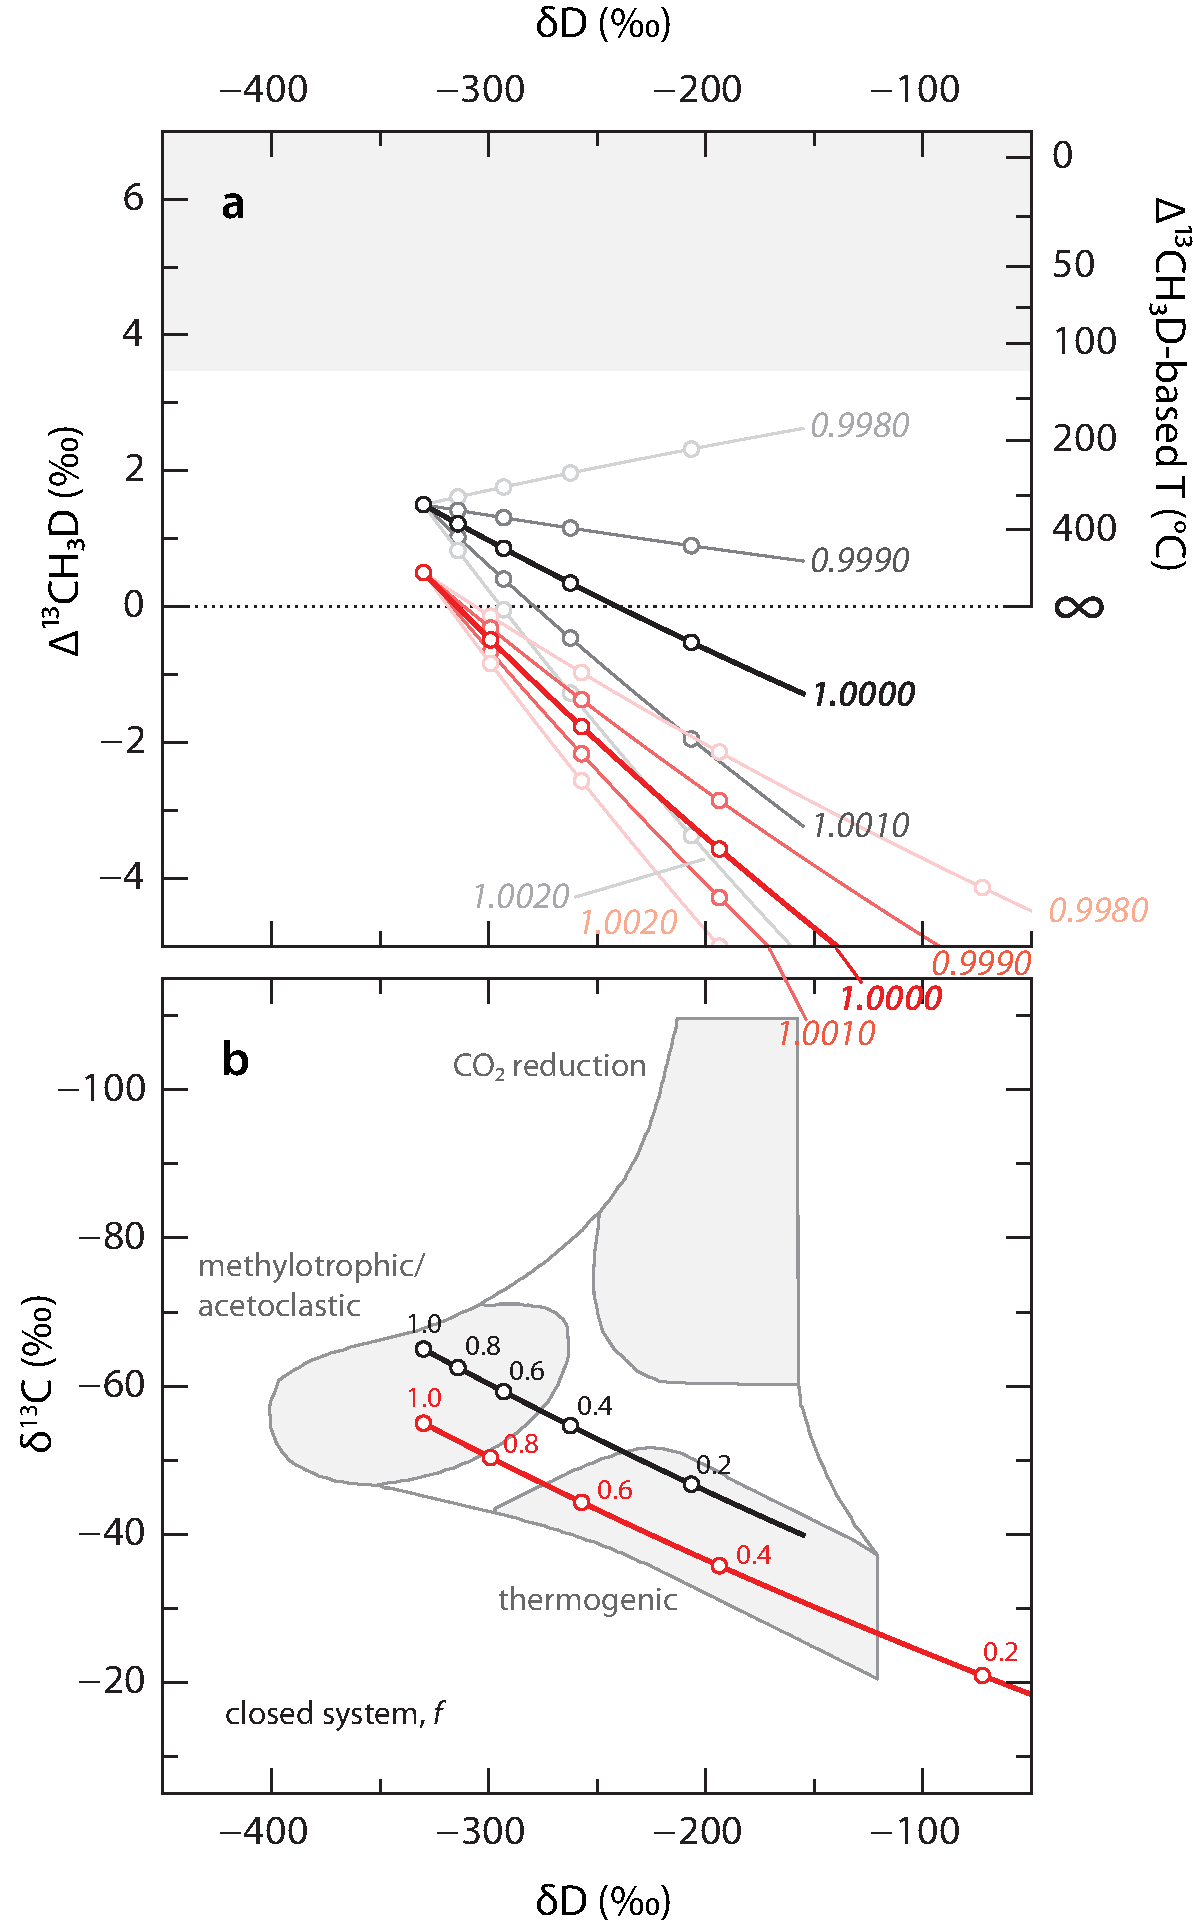
\includegraphics[width=0.5\textwidth]{figures/Fig4.3}
	\caption[Trajectories for isotope/isotopologue ratios of methane oxidized in a closed system]{Modeled changes in \textbf{(a)}
		Δ\textsuperscript{13}CH\textsubscript{3}D vs.\ δD and \textbf{(b)}
		δ\textsuperscript{13}C vs.\ δD of residual methane during aerobic methane
		oxidation under closed system conditions. Solid lines represent model
		predictions (from \mrefs[]{Eqns.}{eqn:4:13}, \ref{eqn:4:16}, and~\ref{eqn:4:20}) based on the calculated
		weighted-average carbon- and hydrogen-isotope fractionation factors for
		each set of experiments (black, 30~°C; red, 37~°C) as listed in \autoref{tab:4:1}
		and shown in \autoref{fig:4:1}. Labels in \emph{italics} in panel (a) represent $\gamma$
		values. Circles are marked at intervals of 0.2 in \emph{f}, the fraction
		of initial methane remaining, and labeled in panel (b). For visual
		clarity, the models were initialized at slightly different
		δ\textsuperscript{13}C and Δ\textsuperscript{13}CH\textsubscript{3}D
		values. The initial isotope values were chosen for illustrative purposes
		only and do not represent any particular natural sample; however, the
		chosen values are typical of modern microbial methane generated in
		wetland and lake sediments. Following \textcite{Wang++_2015_S}, the gray field
		in panel (a) represents the temperature range within which microbial
		life has been shown to occur \parencite{Takai++_2008_PNAS}, and the gray fields
		in panel (b) represent empirical methane source fields suggested by
		\textcite{Whiticar_1999_CG}.}
	\label{fig:4:3}
\end{SCfigure*}


In our batch culture experiments, the
Δ\textsuperscript{13}CH\textsubscript{3}D value of residual methane
decreased with progressive oxidation (\autoref{tab:4:1}). The weighted average $\gamma$
values determined for the both the 30~°C experiment (1.0005 ± 0.0006,
2$\sigma$) and the 37~°C experiment (1.0000 ± 0.0014) are indistinguishable
from unity. Thus, the results of this study indicate that the overall
kinetic fractionation factor for
\textsuperscript{13}CH\textsubscript{3}D/\textsuperscript{12}CH\textsubscript{4}
can be closely approximated as the product of the carbon and hydrogen
isotopic fractionation factors (i.e., \textsuperscript{13--D}$\alpha$ $\approx$
\textsuperscript{13}$\alpha$ $\cdot$ \textsuperscript{D}$\alpha$). This product rule can be
used to model the Δ\textsuperscript{13}CH\textsubscript{3}D value
resulting from aerobic methane oxidation. If a higher level of
prediction is necessary, precise constraints on primary and secondary $\alpha$
and $\gamma$ values are required (see \autoref{sec:4:13ch3d-fractionation} and discussion below).

Given low enough $\gamma$ values (depending on \textsuperscript{13}$\alpha$ and
\textsuperscript{D}$\alpha$), the Δ\textsuperscript{13}CH\textsubscript{3}D
value may actually \emph{increase} over the course of the reaction in a
closed system such as a batch culture. The break-even condition, under
which Δ\textsuperscript{13}CH\textsubscript{3}D does not change during a closed system process, occurs when
\(\gamma = \left.{\left({}_{}^{13}\alpha +{}_{}^{\mathrm{D}}\alpha - 1 \right)}\middle/{\left({}_{}^{13}\alpha \cdot{}_{}^{\mathrm{D}}\alpha \right)}\right.\).
For the 30 and 37~°C experiments, the break-even $\gamma$ values are 0.9986 and
0.9943, respectively. These values are substantially less than those
determined experimentally above (the latter by a considerable $-$0.0057 or
$-$5.7‰). Therefore, it should not be assumed that
Δ\textsuperscript{13}CH\textsubscript{3}D values are unaffected by
closed system methane oxidation. Otherwise, the apparent
Δ\textsuperscript{13}CH\textsubscript{3}D temperature may be
substantially overestimated or become imaginary, as shown in \mrefs[a]{Fig.}{fig:4:3}.

There is no \emph{a priori} reason that $\gamma$ must be close to
unity.\footnote{For example, when methane effuses through a small
	orifice, $\gamma$ (when defined as the ratio of the isotopologue
	fractionation factor for
	\textsuperscript{13}CH\textsubscript{3}D/\textsuperscript{12}CH\textsubscript{4}
	to the product of those for
	\textsuperscript{13}CH\textsubscript{4}/\textsuperscript{12}CH\textsubscript{4}
	and
	\textsuperscript{12}CH\textsubscript{3}D/\textsuperscript{12}CH\textsubscript{4})
	will not be unity. From the kinetic theory of gases, the rate of
	effusion of an isotopologue is proportional to
	(mass)\textsuperscript{$-$1/2}, such that $\gamma$ = 1.00174. Escaping methane
	will have lower (lighter) δ\textsuperscript{13}C and δD, but
	\emph{higher} Δ\textsuperscript{13}CH\textsubscript{3}D, than the
	residual methane. For a more thorough discussion, readers are referred
	to \textcite{Eiler+Schauble_2004_GCA}.} The $\gamma$ factor as defined in \autoref{sec:4:13ch3d-fractionation}
is empirically useful in that it is a single number that expresses the
reactivity of \textsuperscript{13}CH\textsubscript{3}D relative to the
other isotopologues. Because \textsuperscript{13}CH\textsubscript{3}D
can react by two nonidentical hydrogen-abstraction reactions (\mrefs[]{Reactions}{eqn:4:8} and \ref{eqn:4:9}), the $\gamma$ value expresses the summation of the products of the
hydrogen-isotope effects (\textsuperscript{D}$\alpha$\textsubscript{p} and
\textsuperscript{D}$\alpha$\textsubscript{s}) and the ``clumped isotopologue
effects'' ($\gamma$\textsubscript{p} and $\gamma$\textsubscript{s}) for D in both
primary and secondary sites:
\(\gamma \cdot{}_{}^{\mathrm{D}}\alpha = \frac{1}{4} \cdot \gamma_{\mathrm{p}} \cdot{}_{}^{\mathrm{D}}\alpha_{\mathrm{p}} + \frac{3}{4} \cdot \gamma_{\mathrm{s}} \cdot{}_{}^{\mathrm{D}}\alpha_{\mathrm{s}}\).
A conceptual exercise helpfully illustrates the relative weighting of D-
vs.\ H-abstraction reactions expressed in the $\gamma$ factor. Assuming
\textsuperscript{D}$\alpha$\textsubscript{p} = 0.02 and
\textsuperscript{D}$\alpha$\textsubscript{s} = 0.9 (from \autoref{sec:4:fractionation-of-methane-13c12c-and-dh-ratios}), and $\gamma$ =
0.9990 (i.e., $-$1‰ from unity, which is at the lower edge of 2$\sigma$
uncertainty on the weighted average $\gamma$ values for the experiments shown
in \autoref{tab:4:1}), then \textsuperscript{D}$\alpha$ = 0.68 and
\(0.6786 = 0.0050 \cdot \gamma_{\mathrm{p}} + 0.6750 \cdot \gamma_{\mathrm{s}}\).
Assigning a value to either $\gamma$\textsubscript{p} or $\gamma$\textsubscript{s}
would constrain the other; hence, two extreme cases can be considered:
(\emph{i}) if $\gamma$\textsubscript{s} = 1, then $\gamma$\textsubscript{p} = 0.86; or
alternatively (\emph{ii}) if $\gamma$\textsubscript{p} = 1, then
$\gamma$\textsubscript{s} = 0.9990. The former case requires a large primary
clumped isotopologue effect because proportionally very few
\textsuperscript{13}CH\textsubscript{3}D (and
\textsuperscript{12}CH\textsubscript{3}D) molecules react through direct
D-abstraction rather than H-abstraction (see \autoref{sec:4:fractionation-of-methane-13c12c-and-dh-ratios}), whereas the
latter requires only a much smaller secondary clumped isotopologue
effect on H-abstraction from \textsuperscript{13}CH\textsubscript{3}D to
explain a $\gamma$ value that deviates slightly from unity. Although
insufficient constraints on either $\gamma$\textsubscript{p} or
$\gamma$\textsubscript{s} are currently available, this exercise indicates that
a small secondary clumped isotopologue effect (i.e., $\gamma$\textsubscript{s}
$\neq$ 1 but is very close) could exist, but may be hardly detectable. Given
the uncertainties surrounding experimental determinations of
\textsuperscript{D}$\alpha$\textsubscript{p} and
\textsuperscript{D}$\alpha$\textsubscript{s} (discussed in \autoref{sec:4:fractionation-of-methane-13c12c-and-dh-ratios}),
accurate values of $\gamma$\textsubscript{p} and $\gamma$\textsubscript{s} cannot yet
be assigned. For geochemical applications, the $\gamma$ factor is at present
best used as an empirically-fitted parameter, similar to the manner in
which the overall D/H fractionation factor \textsuperscript{D}$\alpha$ is
typically treated.

Irrespective of the exact magnitude of the $\gamma$ factor, it is clear that
Δ\textsuperscript{13}CH\textsubscript{3}D becomes less clumped with
progressive oxidation in a closed system under the growth conditions
tested in this study. Because of the consistency of our
\textsuperscript{D}$\varepsilon$/\textsuperscript{13}$\varepsilon$ results with previous
experiments with organisms also using pMMO and/or sMMO (\mrefs[a]{Fig.}{fig:4:2}), it is
not unreasonable to expect similar results on
Δ\textsuperscript{13}CH\textsubscript{3}D values for methane oxidation
by other strains of aerobic methanotrophic bacteria.

As mentioned above (\autoref{sec:4:fractionation-of-methane-13c12c-and-dh-ratios}), a possible explanation for the
differences in the hydrogen isotopic fractionation factor for the
experiments at the two temperatures relates to partial expression of
equilibrium isotope effects in one or both experiments. Evidence against
this explanation derives from the observation that
Δ\textsuperscript{13}CH\textsubscript{3}D values of residual methane in
both experiments follow the predictions of the product rule (i.e., $\gamma$
values are \textasciitilde{}1); therefore it is unlikely that there is a
greater degree of C--H bond re-equilibration during the course of
reaction in one experiment over another. Thus, clumped isotopologue data
also assist in diagnosing presence or absence of isotope exchange during
enzymatic abstraction of H from methane by MMO, and are consistent with
a minor (not detectable) degree of reversibility for this process. The
minor degree of reversibility indicated by the data for aerobic methane
oxidation here contrasts sharply with the anaerobic oxidation of methane
(AOM), an oxidation process in which much greater degrees of
reversibility have been demonstrated using carbon and hydrogen isotopes
\parencite{Holler++_2011_PNAS,Yoshinaga++_2014_NG}. The environmental
implications are discussed in \autoref{sec:4:13ch3d-as-an-environmental-tracer-of-methane-sink-processes}.

\subsection{Implications for biogeochemical systems
}\label{sec:4:implications-for-biogeochemical-systems}

\subsubsection{Methane isotope and isotopologue fractionation in open
	systems}\label{sec:4:methane-isotope-and-isotopologue-fractionation-in-open-systems}


\begin{SCfigure*}
	\centering
	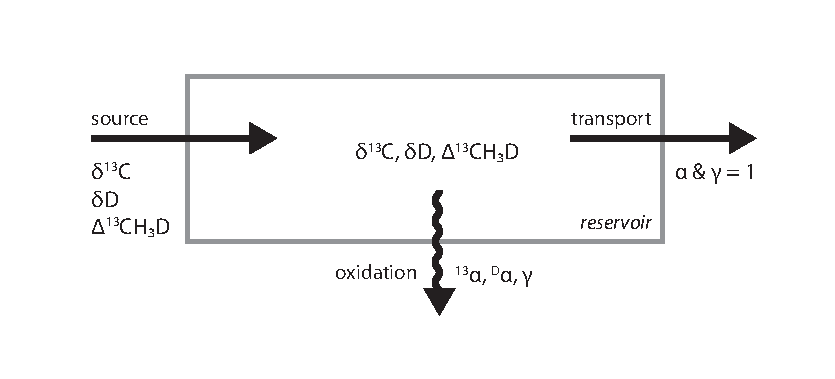
\includegraphics[width=0.7\textwidth]{figures/Fig4.4}
	\caption[Box model for a methane reservoir with transport and oxidation]{Representation of a model open system in which methane
		is transported in and out via advection, and in which aerobic methane
		oxidation is also occurring. The fractional contribution of oxidation to
		the total sinks is $\varphi$\textsubscript{ox}. See \autoref{fig:4:5} and discussion in
		\autoref{sec:4:methane-isotope-and-isotopologue-fractionation-in-open-systems}.}
	\label{fig:4:4}
\end{SCfigure*}


In closed systems, e.g., batch cultures, no steady state is obtained
because of the lack of mass transfer to replenish the methane consumed
by methane oxidation. However, in natural systems operating close to
steady state, there is replenishment of methane from lateral transport
or diffusion, as well as methanogenesis, and there may be multiple
sinks, including methane oxidation and mass transport (\autoref{fig:4:4}).

Experimental alternatives to batch cultures, namely flow-through
bioreactors (chemostats), have been used to more directly approach the
calibration of isotopic fractionation factors due to microbial
metabolism in natural settings. For example, \textcite{Templeton++_2006_GCA}
grew pure and mixed cultures of aerobic methanotrophs in chemostats to
determine the carbon isotope fractionation between methane and product
methanol as a function of environmental and physiological conditions. In
such an open system, there is a constant influx of reactant methane,
which at steady state is balanced by the sum of methane oxidation and
methane carried in the effluent out of the bioreactor (i.e., dilution).


\begin{SCfigure*}
	\centering
	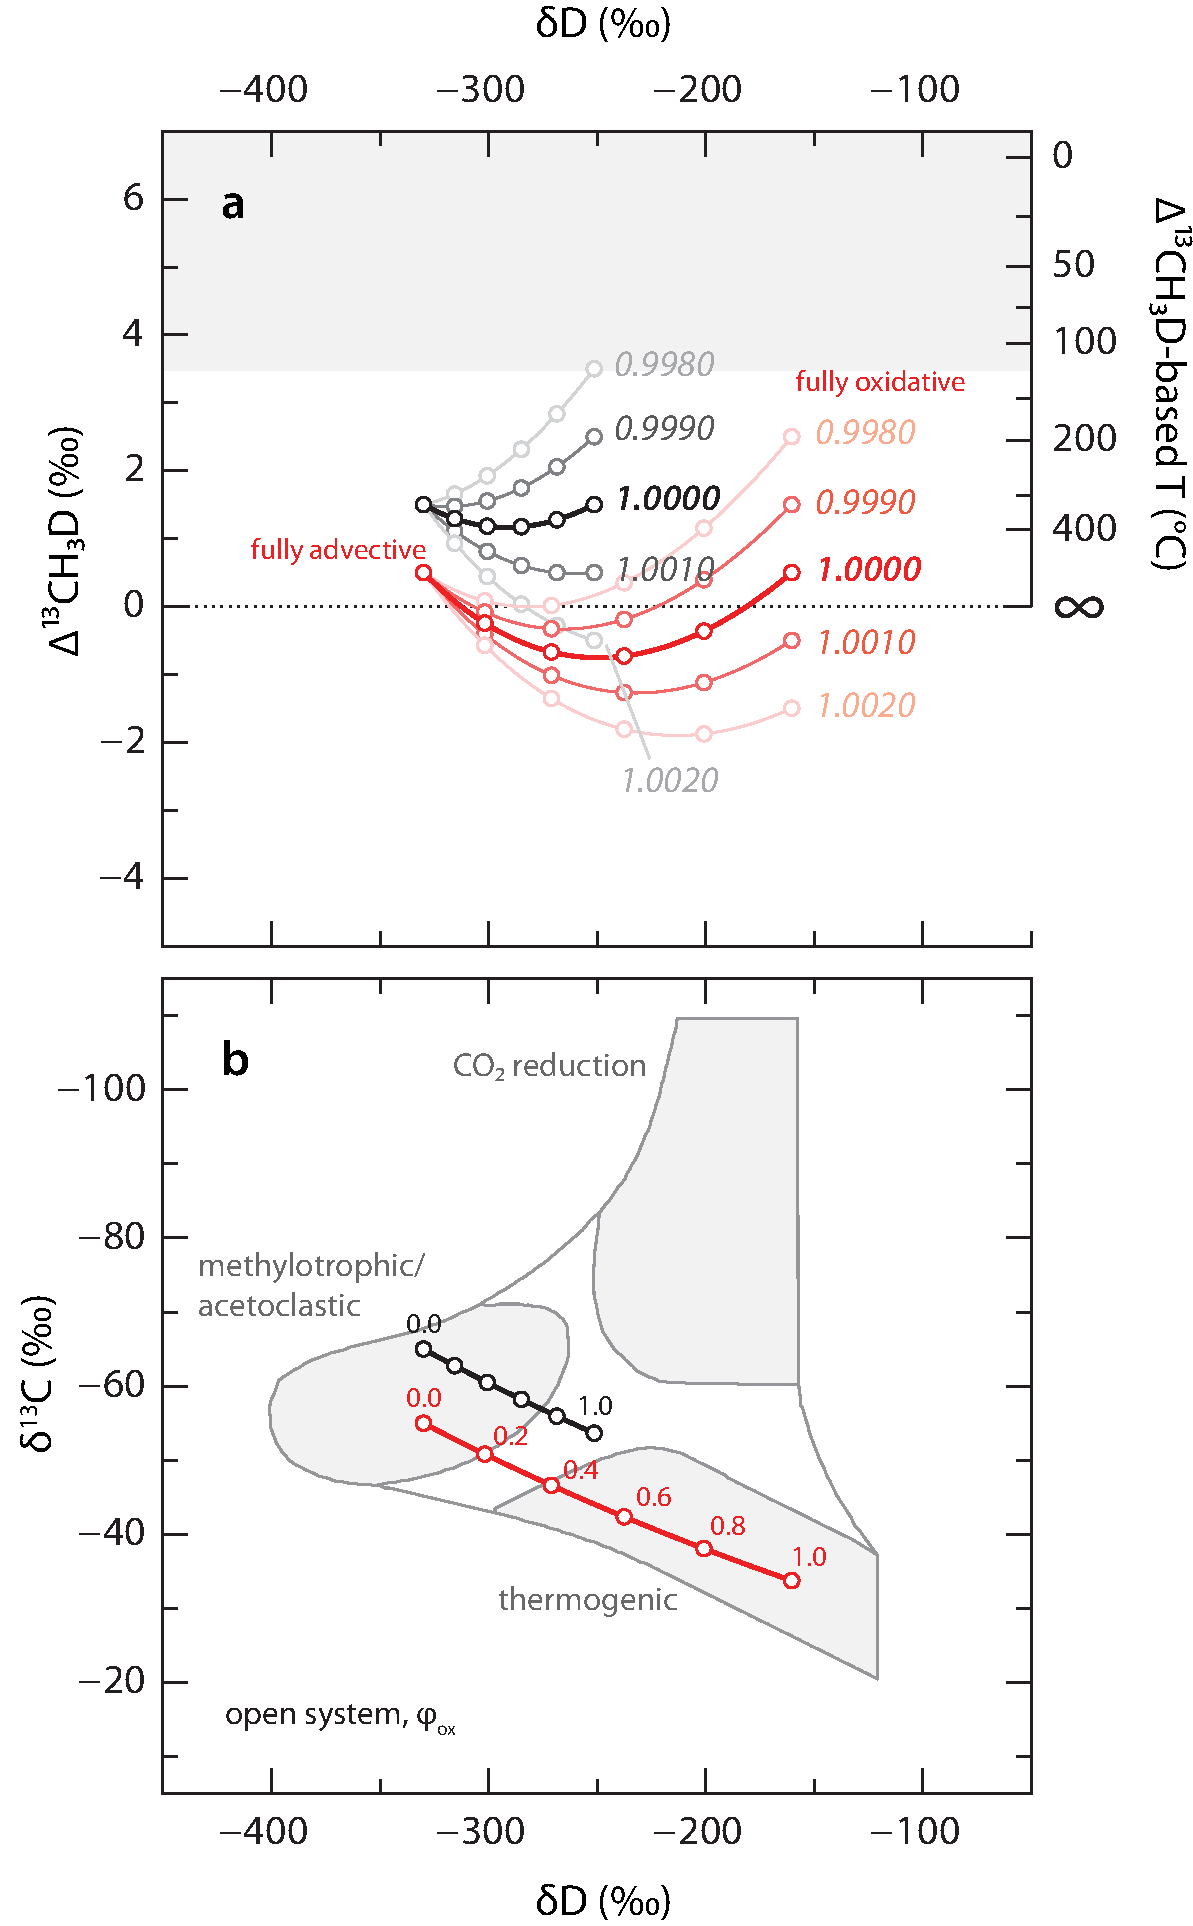
\includegraphics[width=0.5\textwidth]{figures/Fig4.5}
	\caption[Trajectories for isotope/isotopologue ratios of methane oxidized in an open system]{Modeled steady-state values of \textbf{(a)}
		Δ\textsuperscript{13}CH\textsubscript{3}D vs.\ δD and \textbf{(b)}
		δ\textsuperscript{13}C vs.\ δD of methane in an open system (\autoref{fig:4:4})
		consisting of a single source and two sinks (aerobic methane oxidation
		and advection). Advection is assumed to be non-fractionating. Lines were
		modeled using \mrefs[]{Eqns.}{eqn:4:22} and \ref{eqn:4:23}, and the same fractionation factors for
		aerobic methane oxidation as for those shown with the same line style in
		\autoref{fig:4:2}. Labels in \emph{italics} in panel (a) represent $\gamma$ values
		associated with aerobic methane oxidation. Circles are marked at
		intervals of 0.2 in $\varphi$\textsubscript{ox}, the fraction of methane removed
		via oxidation, ranging from fully advective ($\varphi$\textsubscript{ox} = 0) to
		fully oxidative ($\varphi$\textsubscript{ox} = 1), and labeled in panel (b).
		When $\varphi$\textsubscript{ox} = 0, the isotopic composition of methane in the
		reservoir is identical to that of the source. For visual clarity, the
		calculations were performed for slightly different
		δ\textsuperscript{13}C and Δ\textsuperscript{13}CH\textsubscript{3}D
		values of input methane. For description of shaded fields, see the
		caption for \autoref{fig:4:3}.}
	\label{fig:4:5}
\end{SCfigure*}

In the simple limiting case where the fraction of methane removed by
oxidation approaches 100\% (i.e., no methane escapes the system intact),
there is effectively one sink of methane, with fractionation factors
\textsuperscript{13}$\alpha$, \textsuperscript{D}$\alpha$, and $\gamma$ accompanying the
removal process. At steady state, the isotopic values of methane in the
bioreactor would be δ\textsuperscript{13}C =
(δ\textsuperscript{13}C\textsubscript{in} + 1) \big/ \textsuperscript{13}$\alpha$ $-$
1 and δD = (δD\textsubscript{in} + 1) \big/ \textsuperscript{D}$\alpha$ $-$ 1, where
δ\textsubscript{in} represents the isotopic composition of the influent
methane. For \textsuperscript{13}CH\textsubscript{3}D, it can be shown
that
\begin{equation}\label{eqn:4:21}
\Delta_{}^{\mathrm{13}}{\mathrm{C}\mathrm{H}_{\mathrm{3}}\mathrm{D}} = {\Delta_{}^{\mathrm{13}}{\mathrm{C}\mathrm{H}_{\mathrm{3}}\mathrm{D}}}_{\mathrm{\text{in}}} - \ln\gamma\
\end{equation}
as presented in \textcite{Joelsson++_2015_ACPD}. Since $\gamma$ $\approx$ 1, this expression can
be approximated by Δ\textsuperscript{13}CH\textsubscript{3}D~= Δ\textsuperscript{13}CH\textsubscript{3}D\textsubscript{in}~$- (\gamma - 1$).
In our batch culture experiments at 30 and 37~°C, respectively,
weighted-average values for ($\gamma - 1$) of +0.5 ± 0.3‰ and 0.0 ± 0.7‰ (1$\sigma$)
were obtained (\autoref{tab:4:1}). Although steady-state experiments were not
conducted in the current study, if it is assumed that these values are
also characteristic of true open-system isotopologue fractionation
factors, then the above expression can be used to place bounds on the
isotopologue composition of methane in the limiting case outlined above.
Examples of the calculated methane isotopic/isotopologue compositions
are shown for model scenarios in \mrefs[a]{Fig.}{fig:4:5} (corresponding to the endmember
labeled ``fully oxidative'' on each curve).

\mrefs[]{Equation}{eqn:4:21} also shows that in a system at steady state where methane is
solely removed by one process (here, oxidation), the
Δ\textsuperscript{13}CH\textsubscript{3}D value is determined solely by
the Δ\textsuperscript{13}CH\textsubscript{3}D value of the methane
source and the $\gamma$ factor, in contrast to closed systems where
Δ\textsuperscript{13}CH\textsubscript{3}D of residual methane is
influenced also by the isotopic fractionations for bulk
\textsuperscript{13}C/\textsuperscript{12}C and D/H. However, in more
complex systems with multiple removal processes and associated
fractionation factors, the partitioning of flows among the removal
processes must be considered \parencite{Hayes_2001_RiMG}.

One example of such an open system is shown in \autoref{fig:4:4}. Here, methane is
carried into the system via advection, and removed by both advection and
oxidation. Oxidation of methane has associated fractionation factors
\textsuperscript{13}$\alpha$, \textsuperscript{D}$\alpha$, and $\gamma$, whereas transport
processes are assumed to cause no fractionation \parencite{Alperin++_1988_GBC},
i.e., values of $\alpha$ and $\gamma$ are unity. The fraction of methane removed via
oxidation, $\varphi$\textsubscript{ox}, describes the partitioning of flows
among the two methane sinks. It can be shown that at steady state, the
hydrogen isotopic composition of the methane in the reservoir is \parencite{Hayes_2001_RiMG}:
\begin{equation}\label{eqn:4:22}
\mathrm{\text{δD}} = \ \frac{\mathrm{\text{δD}}_{\mathrm{\text{in}}} + 1}{1 + \varphi_{\mathrm{\text{ox}}}\left({}_{}^{\mathrm{D}}\alpha - 1 \right)} - 1
\end{equation}

An analogous equation (not shown) describes the carbon isotopic
composition of methane in this system at steady state. When the
δ\textsuperscript{13}C and δD values are plotted against each other, it
can be seen that the trajectory describing the continuum between the
fully-advective ($\varphi$\textsubscript{ox} = 0) and fully-oxidative
($\varphi$\textsubscript{ox} = 1) endmembers is slightly curved (though
approximately linear at most scales of interest, \mrefs[b]{Fig.}{fig:4:5}).

For this system, unlike in the simple fully-oxidative case described by \autoref{eqn:4:21}, the abundance of \textsuperscript{13}CH\textsubscript{3}D is affected not only by the $\gamma$ value, but also by
the \textsuperscript{13}$\alpha$ and \textsuperscript{D}$\alpha$ values:
\begin{equation}\label{eqn:4:23}
\Delta_{}^{\mathrm{13}}{\mathrm{C}\mathrm{H}_{\mathrm{3}}\mathrm{D}} = {\Delta_{}^{\mathrm{13}}{\mathrm{C}\mathrm{H}_{\mathrm{3}}\mathrm{D}}}_{\mathrm{\text{in}}} - \ln\frac{1 + \varphi_{\mathrm{\text{ox}}}\left( \gamma \cdot{}_{}^{13}\alpha \cdot{}_{}^{\mathrm{D}}\alpha - 1 \right)}{\left( 1 + \varphi_{\mathrm{\text{ox}}}\left({}_{}^{13}\alpha - 1 \right) \right)\left( 1 + \varphi_{\mathrm{\text{ox}}}\left({}_{}^{\mathrm{D}}\alpha - 1 \right) \right)}\ 
\end{equation}

This results in a parabolic curve connecting the fully-advective and
fully-oxidative endmembers (\mrefs[a]{Fig.}{fig:4:5}). For aerobic methane oxidation, the
curvature on \mrefs[a]{Fig.}{fig:4:5} is always expected to be concave up, because both
the \textsuperscript{13}$\alpha$ and \textsuperscript{D}$\alpha$ values are less than
unity. The relative position of the endmembers in
Δ\textsuperscript{13}CH\textsubscript{3}D space is determined by the $\gamma$
value. When $\varphi$\textsubscript{ox} = 1, \autoref{eqn:4:23} reduces to \autoref{eqn:4:21}.

\subsubsection{\texorpdfstring{Δ\textsuperscript{13}CH\textsubscript{3}D as
		an environmental tracer of methane sink
		processes}{Δ13CH3D as an environmental tracer of methane sink processes}}\label{sec:4:13ch3d-as-an-environmental-tracer-of-methane-sink-processes}

Both biological and chemical processes are important sinks in the
methane budget. In terrestrial ecosystems and oxygenated marine water
columns, aerobic methanotrophy dominates, whereas in sulfate-rich marine
sediments and gas seeps, anaerobic consumption of methane becomes
important \parencite{Cicerone+Oremland_1988_GBC,Reeburgh_2007_CR,Valentine_2011_ARMar,Boetius+Wenzhoefer_2013_NG}. In the atmosphere, the primary sink
(\textasciitilde{}90\%) is the reaction with tropospheric OH, with small
contributions from microbial oxidation in soils, loss to stratosphere,
and reaction with tropospheric Cl \parencite{Kirschke++_2013_NG}.

These methane-consuming processes impart distinct carbon- and
hydrogen-isotopic fractionations. In general, biological processes
(including aerobic methane oxidation, anaerobic oxidation of methane,
and nitrite-dependent anaerobic methane oxidation) have
\textsuperscript{D}$\varepsilon$/\textsuperscript{13}$\varepsilon$ ratios between 6 and 15,
whereas the atmospheric sinks, CH\textsubscript{4} + OH and
CH\textsubscript{4} + Cl, have
\textsuperscript{D}$\varepsilon$/\textsuperscript{13}$\varepsilon$ ratios \textasciitilde{}58
and \textasciitilde{}5.5, respectively (\autoref{tab:4:2}). The consistent and
sizable differences in isotopic behavior among the two atmospheric
processes vs.\ biological processes is useful for constraining the
balance of different sources and sinks of methane \parencite[e.g.,][]{Kai++_2011_N,Rigby++_2012_JGR,Whiticar+Schaefer_2007_PTRSA}.

The behavior of methane clumped isotopologues in atmospheric reactions
has also been studied. Recently, \textcite{Joelsson++_2014_CPL} and \textcite{Joelsson++_2016_ACP} reported the fractionation factor for
\textsuperscript{13}CH\textsubscript{3}D in relative-rate experiments on
the reactions of Cl and OH, respectively. Their experiments were
conducted with mixtures of \textsuperscript{12}CH\textsubscript{4} and
\textsuperscript{13}CH\textsubscript{3}D (and also
\textsuperscript{12}CH\textsubscript{3}D in the OH study). Based on
their measurements, the $\gamma$ value associated with methane oxidation by Cl
was 0.980 ± 0.019, and by OH was 0.978 ± 0.028 (2$\sigma$, \autoref{tab:4:2}). The $\gamma$
value for Cl oxidation is slightly less than unity, implying that less
of the \textsuperscript{13}CH\textsubscript{3}D is oxidized than would
be predicted by the product rule, whereas the $\gamma$ value for OH oxidation
is within error of unity. However, the uncertainty on calculated $\gamma$
values is large (ca.\ 20 to 30‰) due to limitations associated with the
experimental setup and detection technique. Because
Δ\textsuperscript{13}CH\textsubscript{3}D in the environment has a ca.
10‰ range \parencite{Wang++_2015_S}, more precise isotopologue-specific
measurements of methane in experiments conducted at natural abundance
will be necessary in order to constrain clumped isotopologue
fractionations in atmospheric contexts. These experiments have been
conducted, and the results are reported in a companion article
\parencite{Whitehill++_2017_GCA}; a summary of their results are shown in \autoref{tab:4:1}.%\hyperref[tab:4:1]{Tables \ref*{tab:4:1}} and \ref{tab:4:2}.

\begin{table}[t]
		\caption[Comparison of \textsuperscript{D}$\varepsilon$/\textsuperscript{13}$\varepsilon$ and $\gamma$ values for various methane sinks]{Comparison of experimentally-determined ratios of carbon- and
			hydrogen-isotope fractionation factors
			(\textsuperscript{D}$\varepsilon$/\textsuperscript{13}$\varepsilon$) and
			\textsuperscript{13}CH\textsubscript{3}D fractionation factors ($\gamma$) for
			different methane sink processes. Uncertainties quoted are ±2$\sigma$ or 95\%
			confidence interval.}
		\label{tab:4:2}
	\centering
	\begin{threeparttable}
		\begin{tabular}{lll}
			\toprule
			& \textsuperscript{D}$\varepsilon$/\textsuperscript{13}$\varepsilon$ & $\gamma$\tabularnewline
			\midrule
			& &\tabularnewline
			\multicolumn{3}{l}{\emph{Aerobic methane oxidation}}\tabularnewline
			Previous work\tnote{a} & 5.9 to 14.9 &\tabularnewline
			This study\tnote{b} & 9.14 ± 0.14 & 1.0004 ±
			0.0006\tabularnewline
			& &\tabularnewline
			\multicolumn{3}{l}{\emph{Anaerobic oxidation of methane (AOM)}}\tabularnewline
			\textcite{Holler++_2009_EMR} & 6.4 to 8.5 &\tabularnewline
			& &\tabularnewline
			\multicolumn{3}{l}{\emph{Nitrite-dependent anaerobic methane oxidation}}\tabularnewline
			\textcite{Rasigraf++_2012_GCA} & 7.8 ± 0.8 &\tabularnewline
			& &\tabularnewline
			\multicolumn{3}{l}{\emph{CH\textsubscript{4} + OH}} \tabularnewline
			\textcite{Saueressig++_2001_JGR} & 58.5 ± 6.6 &\tabularnewline
			\citeauthor{Joelsson++_2016_ACP} (\cite*{Joelsson++_2015_ACPD,Joelsson++_2016_ACP}) & & 0.980 ± 0.038\tabularnewline
			\textcite{Whitehill++_2017_GCA} & 41.3 ± 8.3 & 0.9997 ± 0.0012\tabularnewline
			& &\tabularnewline
			\multicolumn{3}{l}{\emph{CH\textsubscript{4} + Cl}}\tabularnewline
			\textcite{Tyler++_2000_GRL} & 5.51 &\tabularnewline
			\citeauthor{Saueressig++_1995_GRL} (\cite*{Saueressig++_1995_GRL,Saueressig++_1996_GRL}) & 5.50 &\tabularnewline
			\textcite{Feilberg++_2005_IJChemKin} & 5.65 &\tabularnewline
			\textcite{Joelsson++_2014_CPL} & & 0.978 ± 0.051\tabularnewline
			\textcite{Whitehill++_2017_GCA} & 5.56 & 0.9965 ± 0.0007\tabularnewline
			& &\tabularnewline
			\bottomrule
		\end{tabular}
		\begin{tablenotes}
			\item[a] See caption of \mrefs[a]{Fig.}{fig:4:2} for references. Also see
			\textcite{Rasigraf++_2012_GCA} for a compilation of \textsuperscript{13}$\varepsilon$ and
			\textsuperscript{D}$\varepsilon$ values determined for biological methane oxidation
			in cultures and in the environment.
			\item[b] Derived from linear regression
			(\textsuperscript{D}$\varepsilon$/\textsuperscript{13}$\varepsilon$, \mrefs[a]{Fig.}{fig:4:2}) or weighted
			average ($\gamma$) of all timepoints in both experiments in \autoref{tab:4:1}.
		\end{tablenotes}
	\end{threeparttable}

\end{table}


In the present study, $\gamma$ values for aerobic methane oxidation were
determined (1.0004 ± 0.0006, 2$\sigma$, \autoref{tab:4:2}). These values indicate that
the abstraction of H from methane by methane monooxygenase is associated
with little to no reversibility (see discussion in \autoref{sec:4:fractionation-of-13ch3d}). This
interpretation is consistent with the strong energetic favorability of
methane oxidation to methanol and downstream products in the presence of
abundant O\textsubscript{2}, a strong electron acceptor \parencite{Cicerone+Oremland_1988_GBC,Hanson+Hanson_1996_MMBR}.

The new experimental constraints on clumped isotopologue fractionation
during aerobic methane oxidation also afford an opportunity to briefly
evaluate whether aerobic methane oxidation has influenced methane
clumped isotopologue data available in the literature from various
environments. In particular, because methane oxidation demonstrably
produces nonequilibrium clumped isotopologue signatures in both closed
and open systems considered in this study (\mrefs{Figs.}{fig:4:3} and \ref{fig:4:5}, respectively),
the out-of-equilibrium clumped isotopologue signatures in samples from
Upper and Lower Mystic Lakes (Massachusetts, USA), Swamp Y
(Massachusetts, USA), and The Cedars (California, USA) are considered
again here \parencite{Wang++_2015_S}, as well as a sample from a pond at
Caltech for which a related parameter, the Δ\textsubscript{18} value,
was found to be in disequilibrium \parencite{Stolper++_2015_GCA}. At Upper
Mystic Lake (a 20-m deep seasonally-stratified freshwater lake), bubble
traps were deployed \textasciitilde{}2 m above the lake floor; the
deployment of traps at such deep depths, into the oxygen-depleted
hypolimnion \parencite{Peterson_2005_thesis}, was designed to minimize the possibility
of aerobic methane oxidation \parencite{Wang++_2015_S}. At Lower Mystic Lake
(a 24-m deep meromictic density-stratified lake), the monimolimnion
(from which the reported sample was taken) is anoxic \parencite{Wang++_2015_S}, rendering aerobic methane oxidation unlikely. For Swamp Y and the
Caltech pond, the redox state of the sediments from which the methane
bubbles were stirred and extracted is unknown. At The Cedars, the
extremely high levels of H\textsubscript{2} in gases exsolving from the
springs maintains O\textsubscript{2} at vanishingly low levels \parencite[near the
lower bound of H\textsubscript{2}O stability;][]{Morrill++_2013_GCA}.
Taken together, all methane samples from these four sites exhibit narrow
ranges of δ\textsuperscript{13}C values between $-$59‰ and $-$71‰ and δD
values between $-$265‰ and $-$342‰, but carry a wide range of nonequilibrium
Δ\textsuperscript{13}CH\textsubscript{3}D values (from $-$3.4‰ to +3.2‰)
that are consistent within sites but significantly different between
sites \parencite{Wang++_2015_S}, and exhibit isotopologue patterns that do not
discernably resemble those depicted in \mrefs[]{Figs.}{fig:4:3} and \ref{fig:4:5}. Thus, although
aerobic methane oxidation cannot be fully discounted at these four
sites, the experimental constraints provided in the current study do not
contraindicate the assumptions made by \textcite{Wang++_2015_S} and are
consistent with the hypothesis that nonequilibrium
Δ\textsuperscript{13}CH\textsubscript{3}D values in microbial methane in
the environment and in methanogenic cultures studied to date originate
primarily from intrinsic isotopologue effects during the assembly of
C--H bonds during methanogenesis \parencite{Stolper++_2015_GCA,Wang++_2015_S}.

Alternative biological mechanisms for methane oxidation are also
important in the environment. Of particular interest is the
sulfate-dependent anaerobic oxidation of methane (AOM), which is a major
sink of methane in anoxic marine sediments \parencite{Reeburgh_1976_EPSL}. This
process operates via a very different biochemical pathway from that used
by aerobic methanotrophs. While the biochemistry of AOM has not been
fully characterized, it is likely that the enzymatic pathway of AOM is
the reverse of methanogenesis, and involves the same or similar key
enzymes (e.g., methyl-coenzyme M reductase) for addition or removal of H
from single-carbon compounds \parencite{Scheller++_2010_N}. Previously, it was
found that as the reversibility of methanogenesis decreased (controlled
in part by levels of bioavailable H\textsubscript{2}), both the δD and
Δ\textsuperscript{13}CH\textsubscript{3}D values of the generated
methane became lower or more negative \parencite{Wang++_2015_S}; similar
behavior was found in Δ\textsubscript{18} \parencite{Stolper++_2014_S,Stolper++_2015_GCA}. From incubations of enrichment cultures of
microbial consortia performing AOM, \textcite{Holler++_2009_EMR} determined
substantial kinetic isotope fractionations associated with this process
(\textsuperscript{13}$\varepsilon$ = $-$12‰ to $-$36‰ and \textsuperscript{D}$\varepsilon$ = $-$100‰
to $-$230‰). The negative D/H fractionation factor results in the residual
methane becoming enriched in D. Because of the demonstrated high levels
of reversibility of AOM \parencite{Holler++_2011_PNAS} and the re-equilibration
of \textsuperscript{13}C/\textsuperscript{12}C ratios between methane
and inorganic carbon at the sulfate-methane transition zone \parencite{Yoshinaga++_2014_NG}, it seems reasonable to speculate that AOM may produce
clumped isotope signatures distinct from those of methanogenesis
\parencite{Stolper++_2015_GCA}. In particular, the expression of a combination
of kinetic and equilibrium isotope effects may be observed, such that
the observed Δ\textsuperscript{13}CH\textsubscript{3}D value may lie
between that predicted by the product rule and that predicted for
thermodynamic equilibrium. If so, then measurement of
Δ\textsuperscript{13}CH\textsubscript{3}D may provide a way to
differentiate between AOM and aerobic methanotrophy. Alternatively, if
AOM also generates Δ\textsuperscript{13}CH\textsubscript{3}D
approximating the product rule, then the agreement of
\textsuperscript{D}$\varepsilon$/\textsuperscript{13}$\varepsilon$ between AOM \parencite{Holler++_2009_EMR} and aerobic methanotrophs (\autoref{tab:4:2}) suggests that potentially,
microbially-mediated oxidation of methane produces only a small and
predictable range of clumped isotopologue fractionations.

Another process, the recently-identified nitrite-dependent anaerobic
methane oxidation \parencite{Ettwig++_2010_N}, may also be
environmentally-relevant, though its global prevalence has yet to be
established. The bacterium Candidatus \emph{Methylomirabilis oxyfera}
produces molecular oxygen intracellularly from the reduction of nitrite
to nitric oxide \parencite{Ettwig++_2010_N}, in the absence of environmental
O\textsubscript{2}; the generated oxygen is then consumed along with
methane by membrane-bound pMMO through the aerobic pathway. Because of
the biochemical homology of the bond-breaking enzymatic step to that of
aerobic methanotrophy, it is not unreasonable to expect that
nitrite-dependent anaerobic methane oxidation would produce isotopic and
clumped isotopologue patterns similar to those observed in this study.
Indeed, carbon and hydrogen isotope fractionation factors for this
process, as determined from culture experiments \parencite{Rasigraf++_2012_GCA},
correlate in a manner that overlaps with aerobic methane oxidation
(\autoref{tab:4:2}), lending support to this hypothesis.

\section{Conclusions}\label{sec:4:conclusions}

Experimental investigation of the abundance of four methane stable
isotopologues (\textsuperscript{12}CH\textsubscript{4},
\textsuperscript{13}CH\textsubscript{4},
\textsuperscript{12}CH\textsubscript{3}D, and a clumped isotopologue,
\textsuperscript{13}CH\textsubscript{3}D) during oxidation of methane
with O\textsubscript{2} by \emph{Methylococcus capsulatus} (Bath) grown
at 30 and 37~°C indicates that Δ\textsuperscript{13}CH\textsubscript{3}D
values of residual methane decrease systematically over the course of
reaction in batch culture. The isotopologue fractionation factor for
\textsuperscript{13}CH\textsubscript{3}D/\textsuperscript{12}CH\textsubscript{4}
is closely approximated by the product of those for
\textsuperscript{13}CH\textsubscript{4}/\textsuperscript{12}CH\textsubscript{4}
and
\textsuperscript{12}CH\textsubscript{3}D/\textsuperscript{12}CH\textsubscript{4}.
Based on the isotopologue data, no significant degree of
re-equilibration of C--H bonds in methane was detected.

Models were developed for simple scenarios involving variable fluxes of
methane removed due to advection and oxidation. In open systems
operating at steady state, Δ\textsuperscript{13}CH\textsubscript{3}D
values depend on the ratio of methane removed via different processes,
as well as the isotoplogue fractionation factors associated with those
processes, whereas in closed systems,
Δ\textsuperscript{13}CH\textsubscript{3}D values depend also on the
fraction of methane remaining. Qualitative comparisons of model
predictions with available environmental
Δ\textsuperscript{13}CH\textsubscript{3}D data indicate that aerobic
methane oxidation has only minor, if any, influence on microbial methane
samples reported to date to carry nonequilibrium
Δ\textsuperscript{13}CH\textsubscript{3}D values. In combination with
recent experimental and theoretical work on clumped isotopologue
fractionation associated with other methane sinks, the results of this
study provide necessary constraints for the development of
\textsuperscript{13}CH\textsubscript{3}D as a tracer of the
biogeochemical and atmospheric cycling of methane.

\section*{Acknowledgments}
% \addcontentsline{toc}{section}{Acknowledgments}

We thank J.H-C. Wei and W.J. Olszewski for technical assistance, and
D.S. Gruen, R.E. Summons, J.W. Pohl\-man, J.S. Seewald, and A.R. Whitehill
for discussions. D.L. Valentine and two anonymous referees are thanked
for helpful and constructive reviews. Grants from the National Science
Foundation (NSF EAR-1250394 to S.O. and EAR-1451767 to P.V.W.), and the
Deep Carbon Observatory (to S.O.) supported this study. S.O. thanks the
Kerr-McGee Professorship at MIT. This research was conducted with
Government support under and awarded by U.S. Department of Defense,
Office of Naval Research, National Defense Science and Engineering
Graduate (NDSEG) Fellowship (to D.T.W.), 32 CFR 168a.







	\chapter{Summary and Outlook}\label{ch:5}

\begin{figure*}
	\centering
	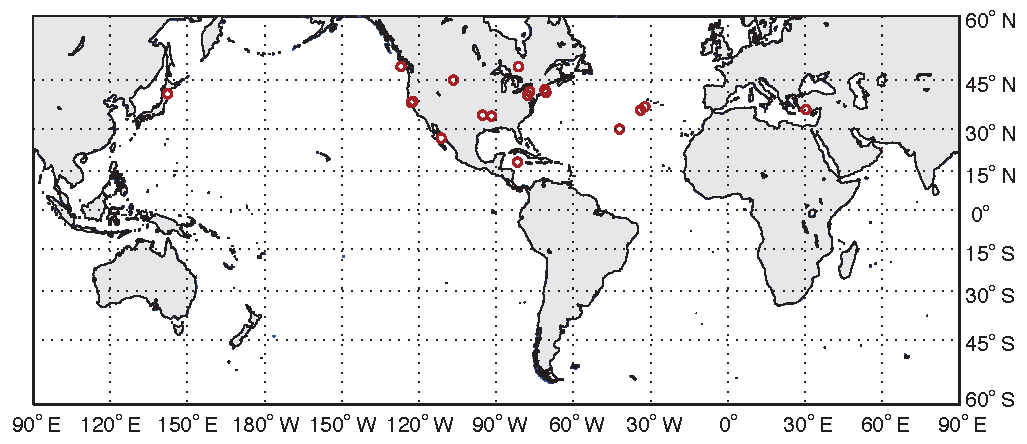
\includegraphics[width=\textwidth]{figures/Fig5.1.pdf}
	\captionsetup{format=myformat}	% hrule beneath caption
	\caption[Map of sample sites investigated by the MIT team]{Map showing locations of sites at which
		Δ\textsuperscript{13}CH\textsubscript{3}D measurements on samples have
		been published or presented from MIT.}
	\label{fig:5:1}
\end{figure*}

The preceding chapters presented a set of data (\autoref{fig:5:1}) that shows
several insights into the origin and fate of the methane stable
isotopologues in the environment. As of the time of writing, methane
clumped isotoplogue data have appeared in at least a dozen articles \parencite{Douglas++_2016_GCA,Stolper++_2014_GCA,Stolper++_2014_S,Stolper++_2015_GCA,Wang++_2015_S,Whitehill++_2017_GCA,Ono++_2014_AC,Wang++_2016_GCA,Lopes++_2016_JoDS,Inagaki++_2015_S,Young++_2016_IJMS,Young++_2017_GCA}.


\begin{SCfigure*}
	\centering
	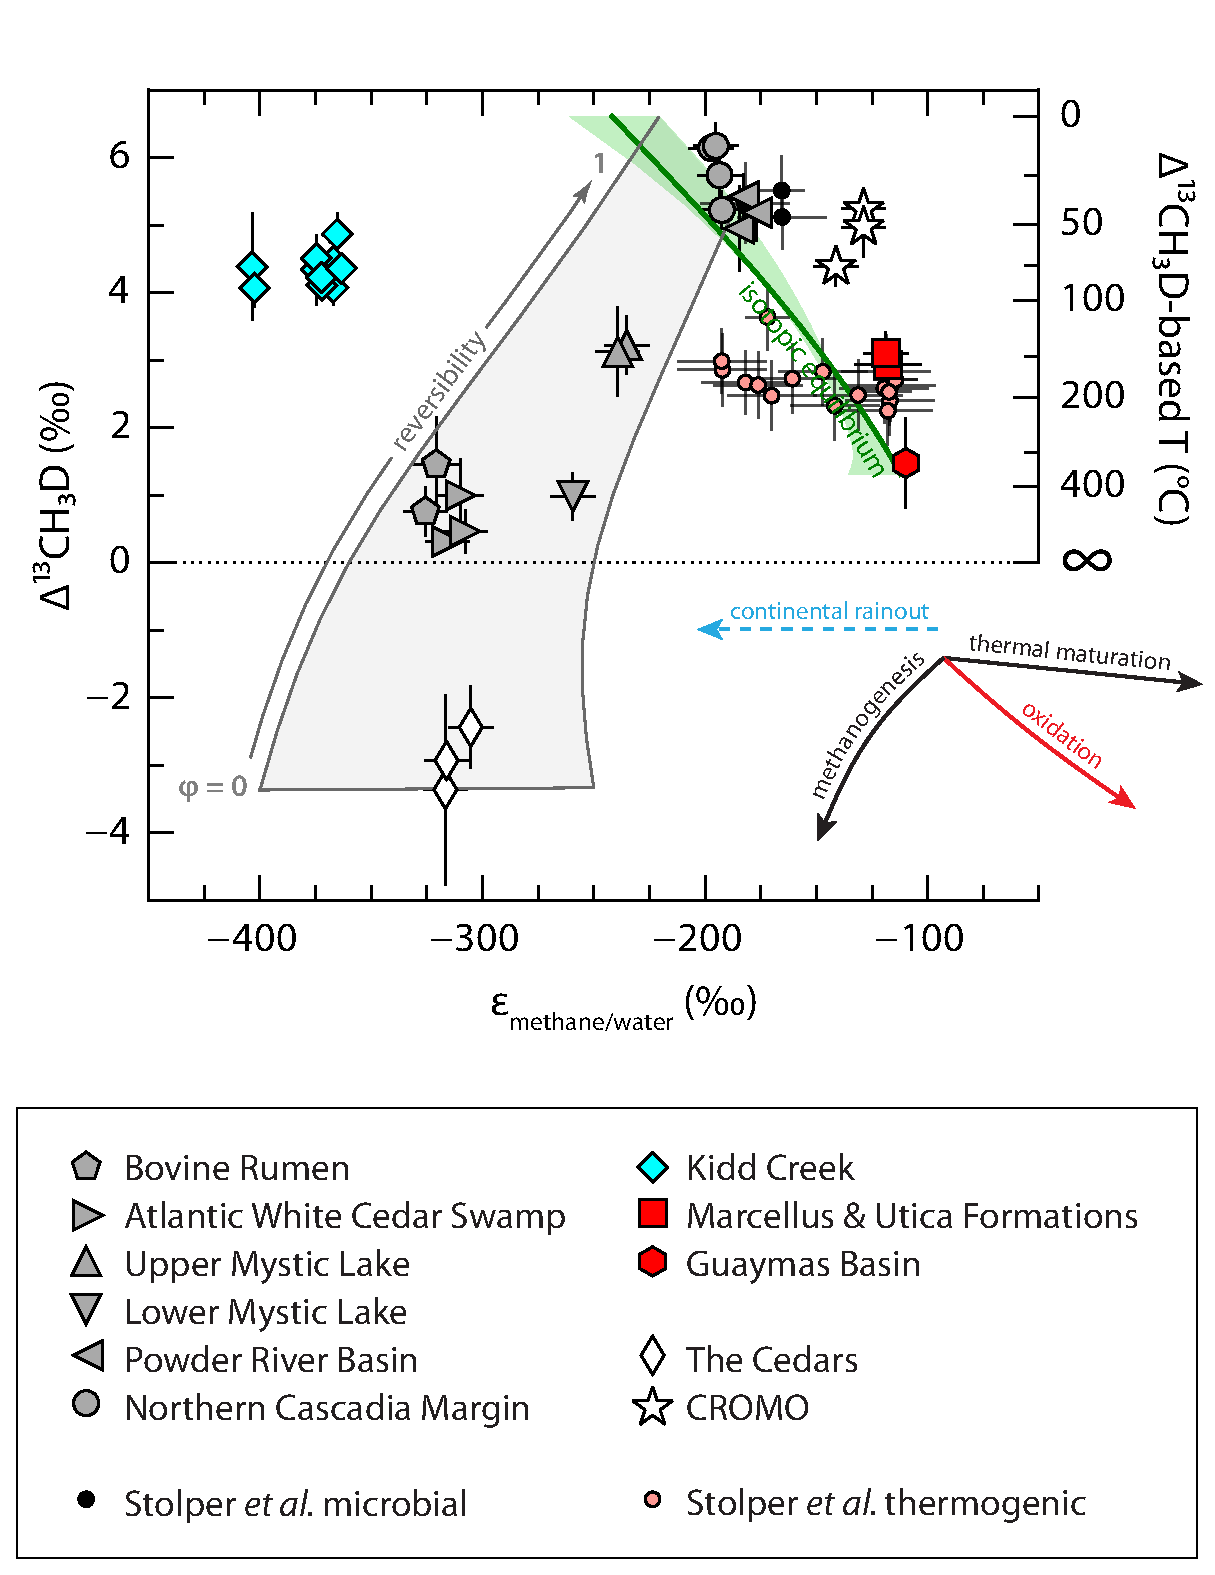
\includegraphics[width=0.57\textwidth]{figures/Fig5.2.pdf}
	\captionsetup{format=myformat}	% hrule beneath caption
	\caption[A survey of \textsuperscript{13}CH\textsubscript{3}D in the environment]{A survey of \textsuperscript{13}CH\textsubscript{3}D in
		the environment. This figure is the same as \autoref{fig:2:2}, with
		the addition of schematic vectors showing basic controls on the isotopic
		signatures of CH\textsubscript{4}, and data from \textcite{Stolper++_2014_S}.
		The position of their data along the \emph{x}-axis was calculated from
		estimated δD of formation waters, and for the \emph{y}-axis,
		Δ\textsubscript{18} values were converted to
		Δ\textsuperscript{13}CH\textsubscript{3}D by assuming equilibrium and
		applying the conversion shown in \mrefs[A]{Fig.}{fig:C:2}.}
	\label{fig:5:2}
\end{SCfigure*}

The Δ\textsuperscript{13}CH\textsubscript{3}D data were shown to be
independent of and complementary to δ\textsuperscript{13}C and δD. A
case was built for why hydrogen (or free energy) exerts a major control
on Δ\textsuperscript{13}CH\textsubscript{3}D and D/H of methane; this
and several other controls are shown in \autoref{fig:5:2}. And several
opportunities for advancement on the technical and theoretical sides of
the problem of methane origin have been highlighted (\autoref{fig:5:3}), including:
\begin{itemize}
	\item
	refining the calibration at low temperatures \parencite{Larson+Hall_1965_JPC,Naito++_2005_ApCat,Golden++_2001_JACS,Robertson++_1975_TFS};
	\item
	experiments to retrieve kinetics associated with the breaking and
	reforming of C--H bonds \parencite{Reeves++_2012_GCA,Lyon+Hulston_1984_GCA,Koepp_1978};
	\item
	construction of numerical models to test hypotheses regarding
	biophysical controls on isotopologue abundances.
\end{itemize}


\begin{figure*}
	\centering
	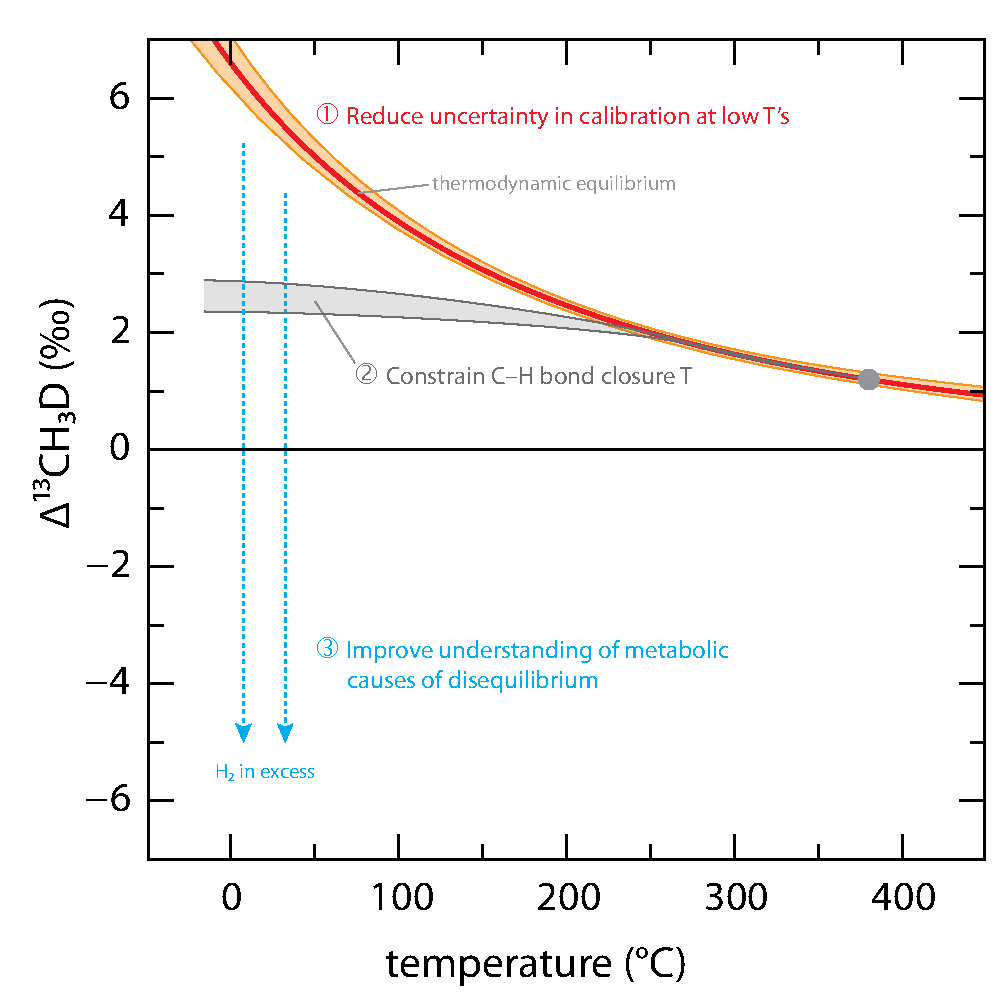
\includegraphics[width=0.5\textwidth]{figures/Fig5.3.pdf}
%	\captionsetup{format=myformat}	% hrule beneath caption
	\caption{Challenges and opportunities in understanding Δ\textsuperscript{13}CH\textsubscript{3}D}
	\label{fig:5:3}
\end{figure*}


Through this work, we have also realized that there is much more
information to be extracted from simple gas chemistry and conventional
stable isotope data than has perhaps been widely appreciated; or that
has been somewhat overlooked in the rush to develop and deploy new
technologies. Measurements of clumped isotopologues provide more
dimensions of data to characterize methane samples, which, as this
thesis shows, does provide additional constraints on certain Earth
systems. However, instruments to measure the doubly-substituted
isotopologues will likely remain a novelty for the foreseeable future.

I suspect that the most significant advances for our understanding of
the origins, transport, and fate of methane are still yet to come. The
biggest steps forward will come with moving away from straightforward
but often restrictive phenomenological representations of legacy data
and towards predictive and quantitative approaches to testing of
well-defined and geologically-plausible hypotheses. Isotopologue data
will certainly play a large role in helping narrow the solution space of
problems of geochemical nature. \mrefs[]{Figures}{fig:5:4} and \ref{fig:5:5} show some attempts at
making such data more easily accessible.


\begin{SCfigure*}
	\centering
	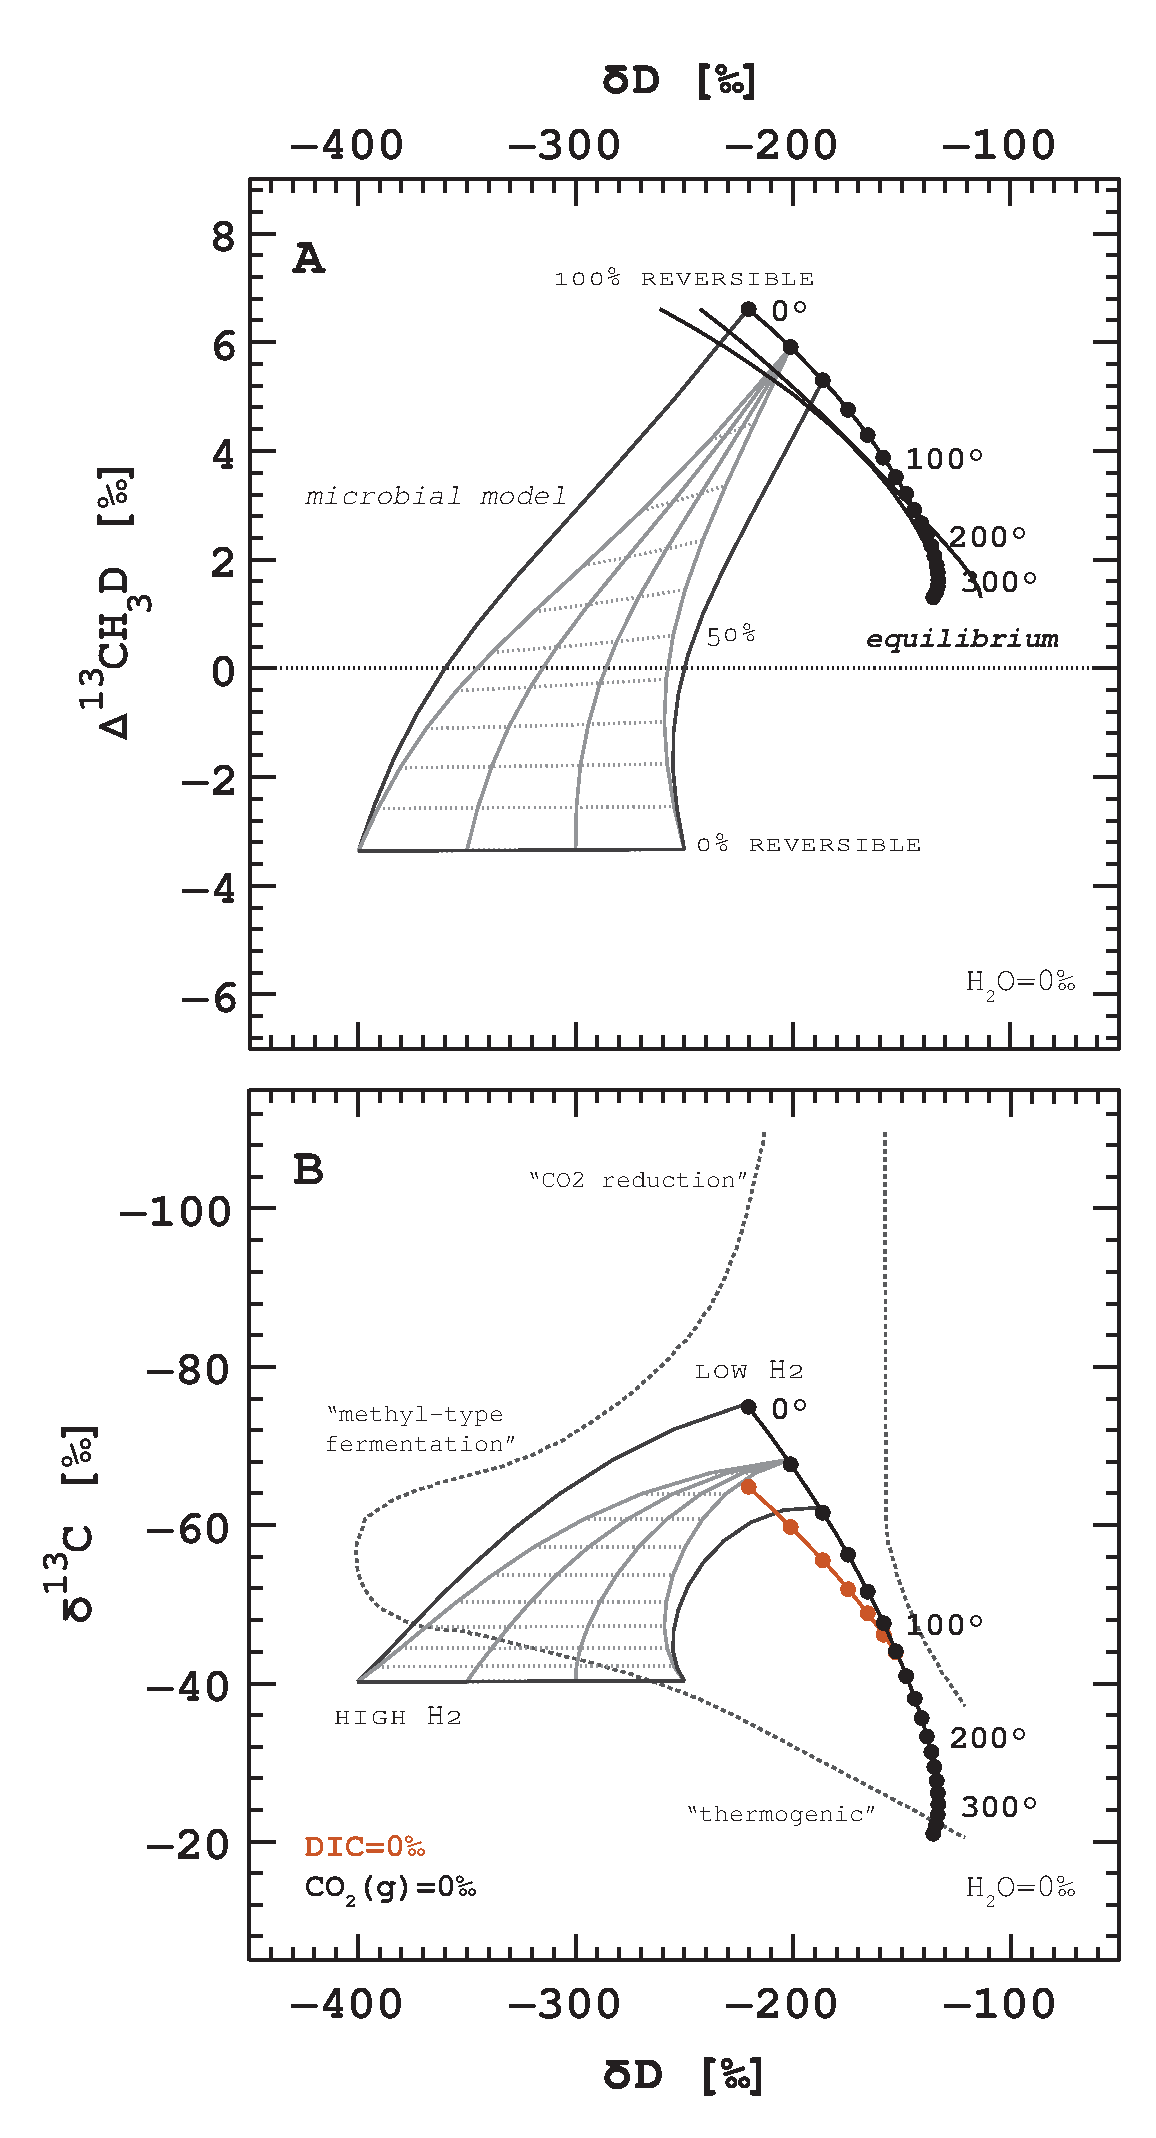
\includegraphics[scale=0.42]{figures/Fig5.4.pdf}
%	\captionsetup{format=myregular}	% no hrule beneath caption
	\caption[Predicted ratios of CH\textsubscript{4} isotopologues
	produced during hydrogenotrophic methanogenesis]{Model of isotopologue abundances in CH\textsubscript{4}
		produced during microbial methanogenesis from
		CO\textsubscript{2}+H\textsubscript{2} \parencite{Wang++_2015_S}. The model
		trajectories begin from a fully-reversible (equilibrium) line whose
		position is determined by assuming δ\textsuperscript{13}C of DIC or
		CO\textsubscript{2} are 0‰ vs.\ PDB. (This assumption is easily changed
		if, for example CO\textsubscript{2} has a higher
		\textsuperscript{13}C/\textsuperscript{12}C ratio than PDB.) The
		underlay in (B) is the outline of the frequently-used plot from \textcite{Whiticar_1990_OG}.
		
		\quad The plot indicates that modeled isotopic compositions for the
		fully-kinetic endmember are enriched in \textsuperscript{13}C and
		depleted in D relative to the equilibrium endmember. The fully-kinetic
		endmember is related to high H\textsubscript{2} concentrations (which
		yield a very large (negative) Δ\textsubscript{r}\emph{G}) \parencite{Burke_1993_Chemosphere}.
		Therefore, hydrogenotrophic methanogens could produce
		CH\textsubscript{4} with isotopic signatures indistinguishable from
		those typically attributed to methylotrophic or acetoclastic
		methanogenesis \parencite{Whiticar_1990_OG,Vinson++_2017_CG}. Whether this is
		true will require evaluation by experiments under low H\textsubscript{2}
		conditions \parencite{Valentine++_2004_GCA,Kawagucci++_2014_GCA,Okumura++_2016_ProgEPS} or \emph{in vitro} \parencite{Scheller++_2013_JACS_KIE}. Caveats to this
		model include (\emph{i}) the assumed fractionation factors may not
		approximate reality well, and (\emph{ii}) the possibility that the
		H-addition steps involved in methanogenesis may be differentially
		reversible in nature.}
	\label{fig:5:4}
\end{SCfigure*}



\begin{figure*}
	\centering
	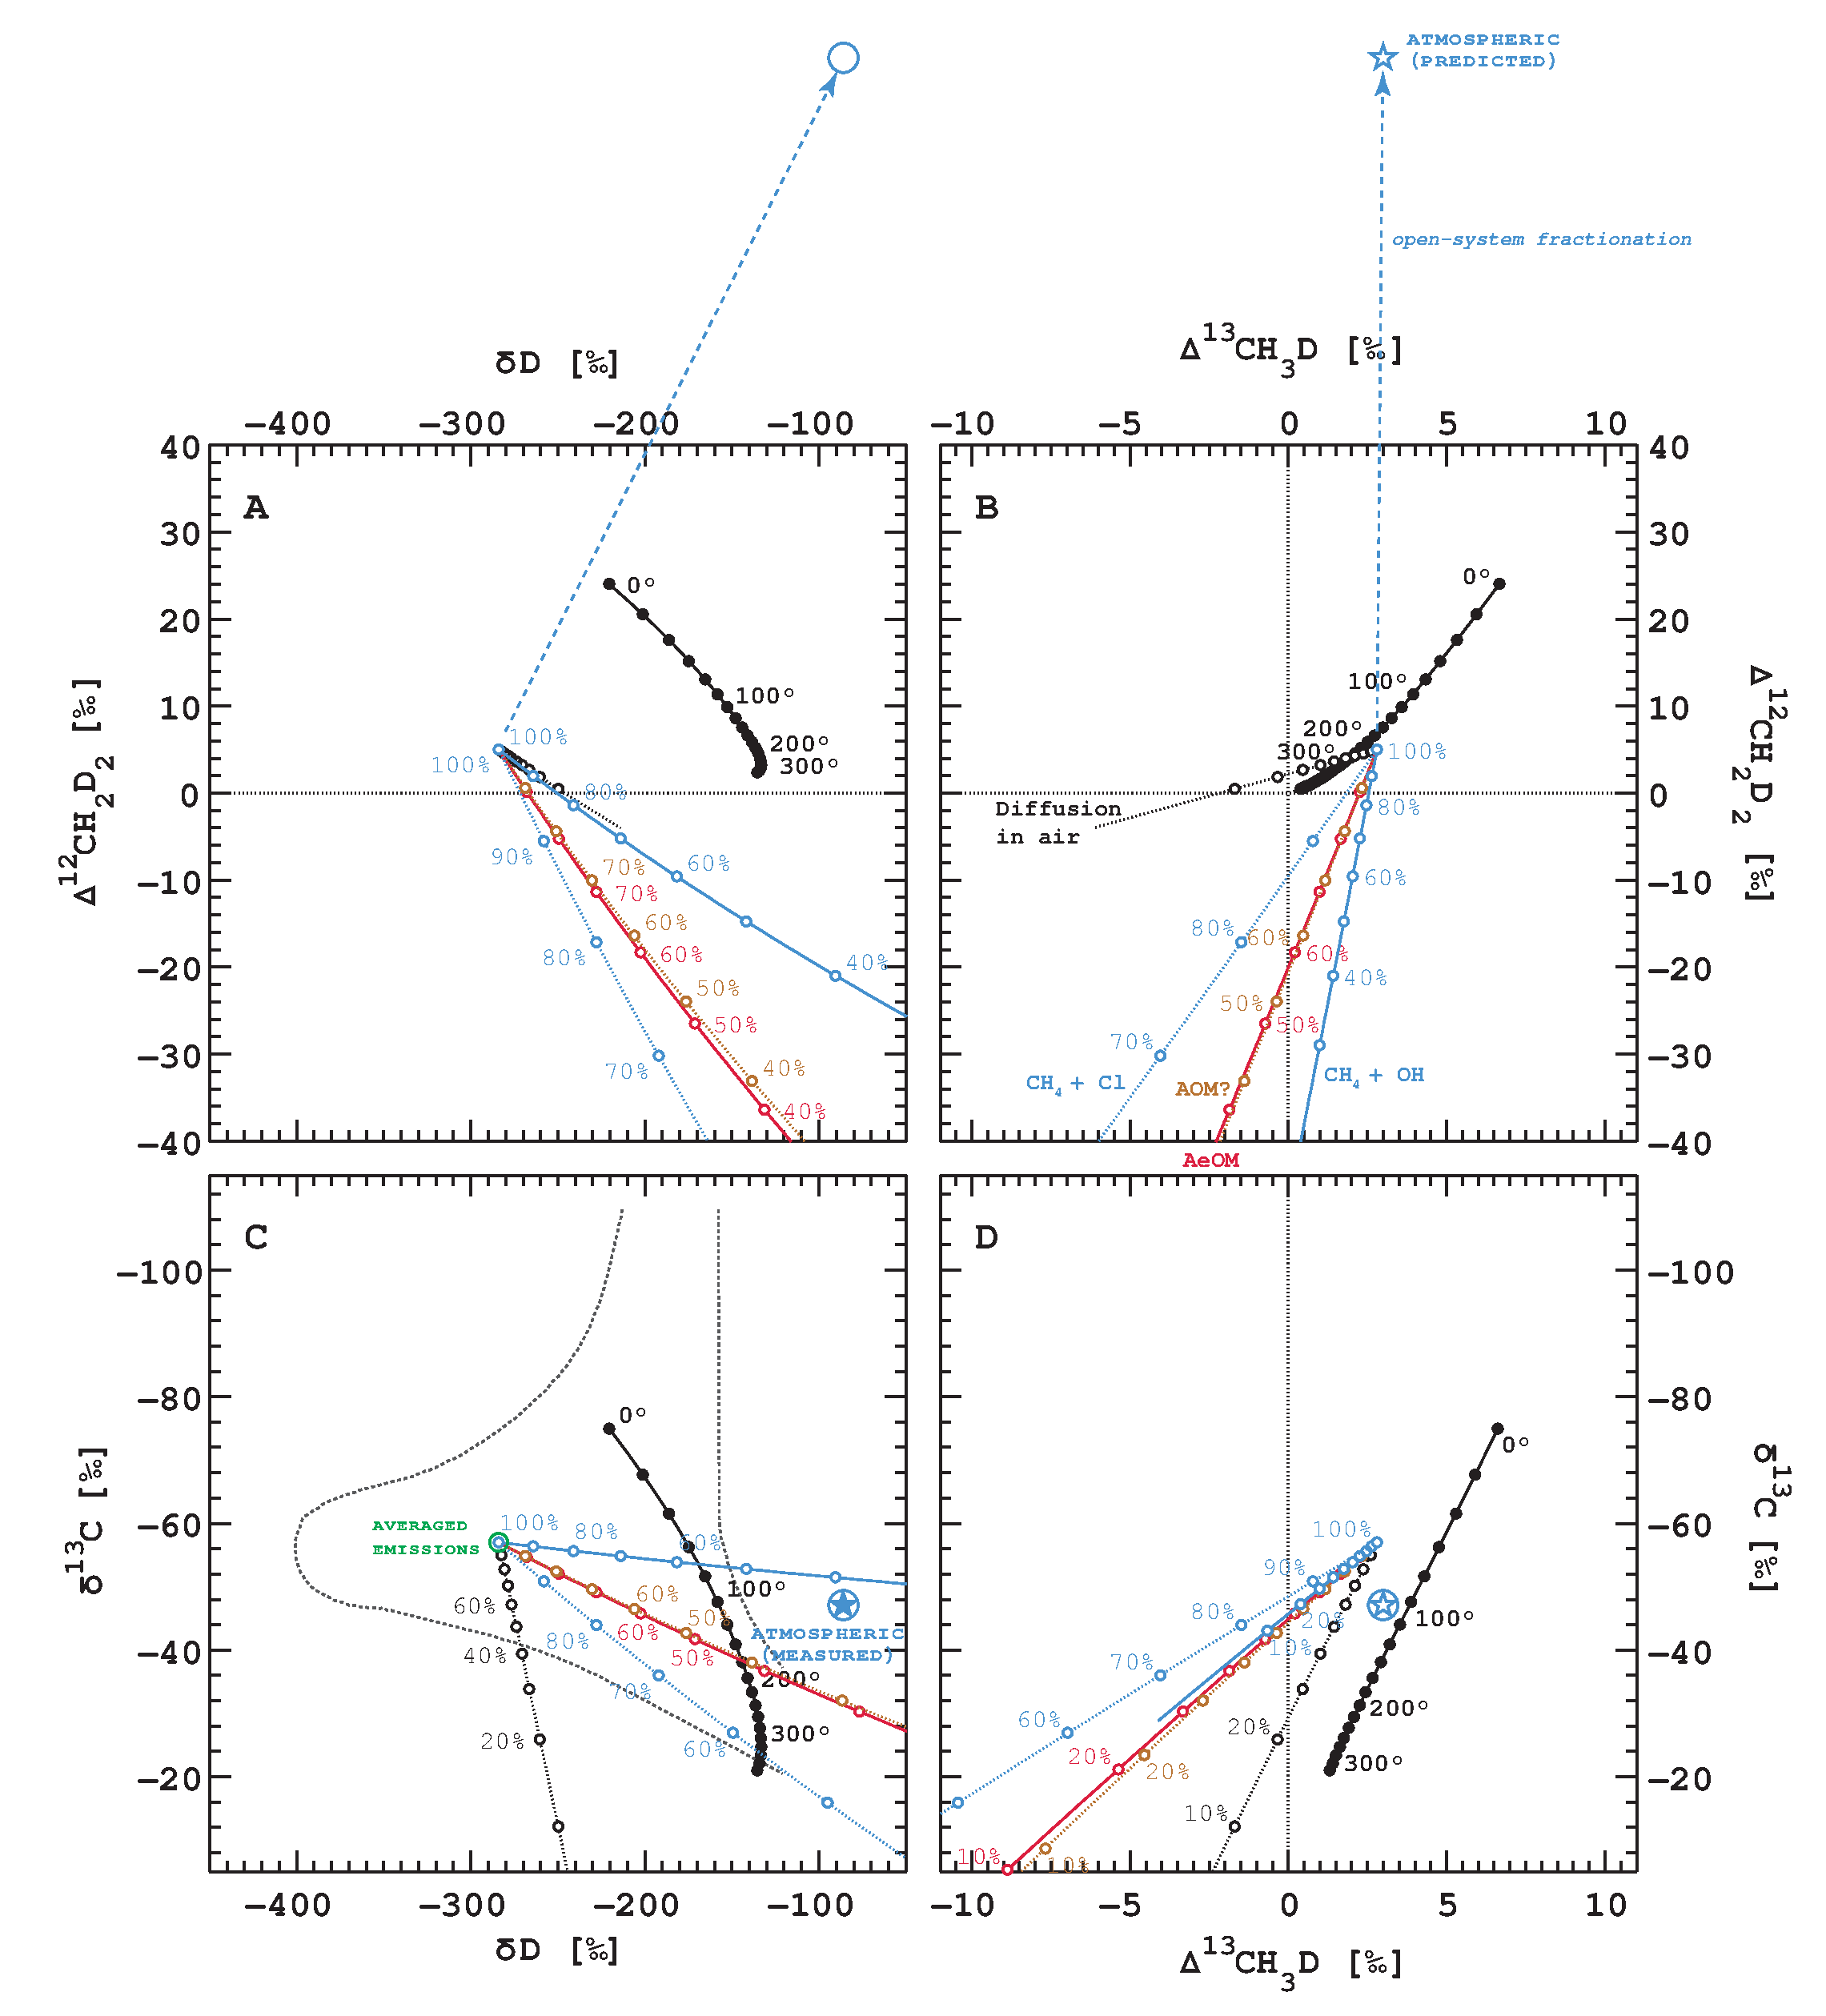
\includegraphics[scale=0.42]{figures/Fig5.5.pdf}
%	\captionsetup{format=myformat}	% hrule beneath caption
	\caption[Behavior of methane isotopologues during methane breakdown]{Evolution of CH\textsubscript{4} isotopologue ratios in
		closed-system, unidirectional bond-breaking processes. Predictions are
		derived from models and/or data presented by the MIT and UCLA teams
		\parencite{Wang++_2016_GCA,Whitehill++_2017_GCA,Young++_2017_GCA}.
		Calculations used the estimated weighted average of modern sources of
		atmospheric methane as the starting point. Trajectory labels indicate
		the fraction of remaining CH\textsubscript{4}. Predictions of
		atmospheric Δ\textsuperscript{13}CH\textsubscript{3}D and
		Δ\textsuperscript{12}CH\textsubscript{2}D\textsubscript{2} assume an
		open system in steady-state. Note that partial reversibility of the
		depicted processes will tend to pull the vectors towards the equilibrium
		line.}
	\label{fig:5:5}
\end{figure*}





	
%	\nopartblankpage
	\appendix
	\appendixpage*
%	\thispagestyle{plain}
%	Text on the following (normally blank page)
%	\clearpage
	
	\chapter[Abundances of methane isotopologues at the Potato
Hills gas field, southeastern
Oklahoma]{Abundances of methane isotopologues at the \\Potato
	Hills gas field, southeastern
	Oklahoma}\label{dx:A}
\chaptermark{Potato Hills}

\begin{abstract}
	\noindent Wells in the Potato Hills region of the Ouachita Mountains, southeastern
	Oklahoma, produce dry natural gas from fractured sandstone units of the
	Pennsylvanian-age Jackfork Group. Previous carbon- and hydrogen-isotope
	measurements of the C\textsubscript{1}--C\textsubscript{4} hydrocarbons
	of these gases revealed that methane is enriched in
	\textsuperscript{13}C and D relative to the C\textsubscript{2+}
	components \parencite{Seewald+Whelan_2005_AAPG-Origin-of-Petroleum}. This pattern of ``isotopic
	reversal'' is commonly-associated with high-maturity gases produced from
	unconventional deep-basin and shale reservoirs \parencite[e.g.,][]{Burruss+Laughrey_2010_OG,Tilley++_2011_AAPGB}, and suggests that gases
	produced in the Potato Hills may have a deep source. However, because of
	the structural complexity of this region, identifying potential source
	rocks and migration pathways has been difficult.
	
	Here, we report additional constraints from tunable infrared laser
	direct-absorption spectroscopy analyses \parencite[see][]{Ono++_2014_AC} of the
	abundance of \textsuperscript{13}CH\textsubscript{3}D (a methane
	``clumped'' isotopologue) in natural gas from the Potato Hills field.
	The measured isotopic signatures are similar across five different wells
	drilled to 1.8--2.3 km depth, suggesting both a common source for the
	methane in these gas samples, and preservation of the C--H bond across
	this \textgreater{}50 km\textsuperscript{2} reservoir system.
	
	Our measurements suggest an apparent \textsuperscript{13}C--D isotopic
	temperature of \textasciitilde{}150 ± 30~°C for methane from the Potato
	Hills field. Application of a model for isotopic exchange suggests that
	migration of thermogenic gases generated at temperatures below 200~°C
	should not result in any detectable reordering of the C--H bonds in
	methane. We discuss uncertainties in the model calibration and
	implications for the preservation of clumped isotopic signatures in
	methane. Results are further interpreted in the context of the regional
	geology to highlight potential implications for natural gas occurrences
	in the Ouachita overthrust belt and beyond.
\end{abstract}

\vspace*{\fill}

\noindent \rule{\textwidth}{0.4pt}\\

{\small
	
	\noindent Preliminary data from this chapter were presented in a talk at the
	24\textsuperscript{th} Annual V.M. Goldschmidt Conference in Sacramento,
	California, USA, June 2014. \\
	
	\noindent This work was done in collaboration with Jeff Seewald (and indirectly,
	Jean Whelan) of WHOI with oversight from Shuhei Ono.
	
}

\clearpage

\section{Introduction}\label{introduction-3}


\begin{sidewaysfigure}
	%	\centering
	\includegraphics[width=\textwidth]{figures/FigA.1.pdf}
	\caption[Map of the frontal and central Ouachita thrust belt]{Relief map of the frontal and central Ouachita
		overthrust belt, southeastern Oklahoma and western Arkansas, USA.}
	\label{fig:A:1}
\end{sidewaysfigure}
\begin{sidewaysfigure}
	%	\centering
	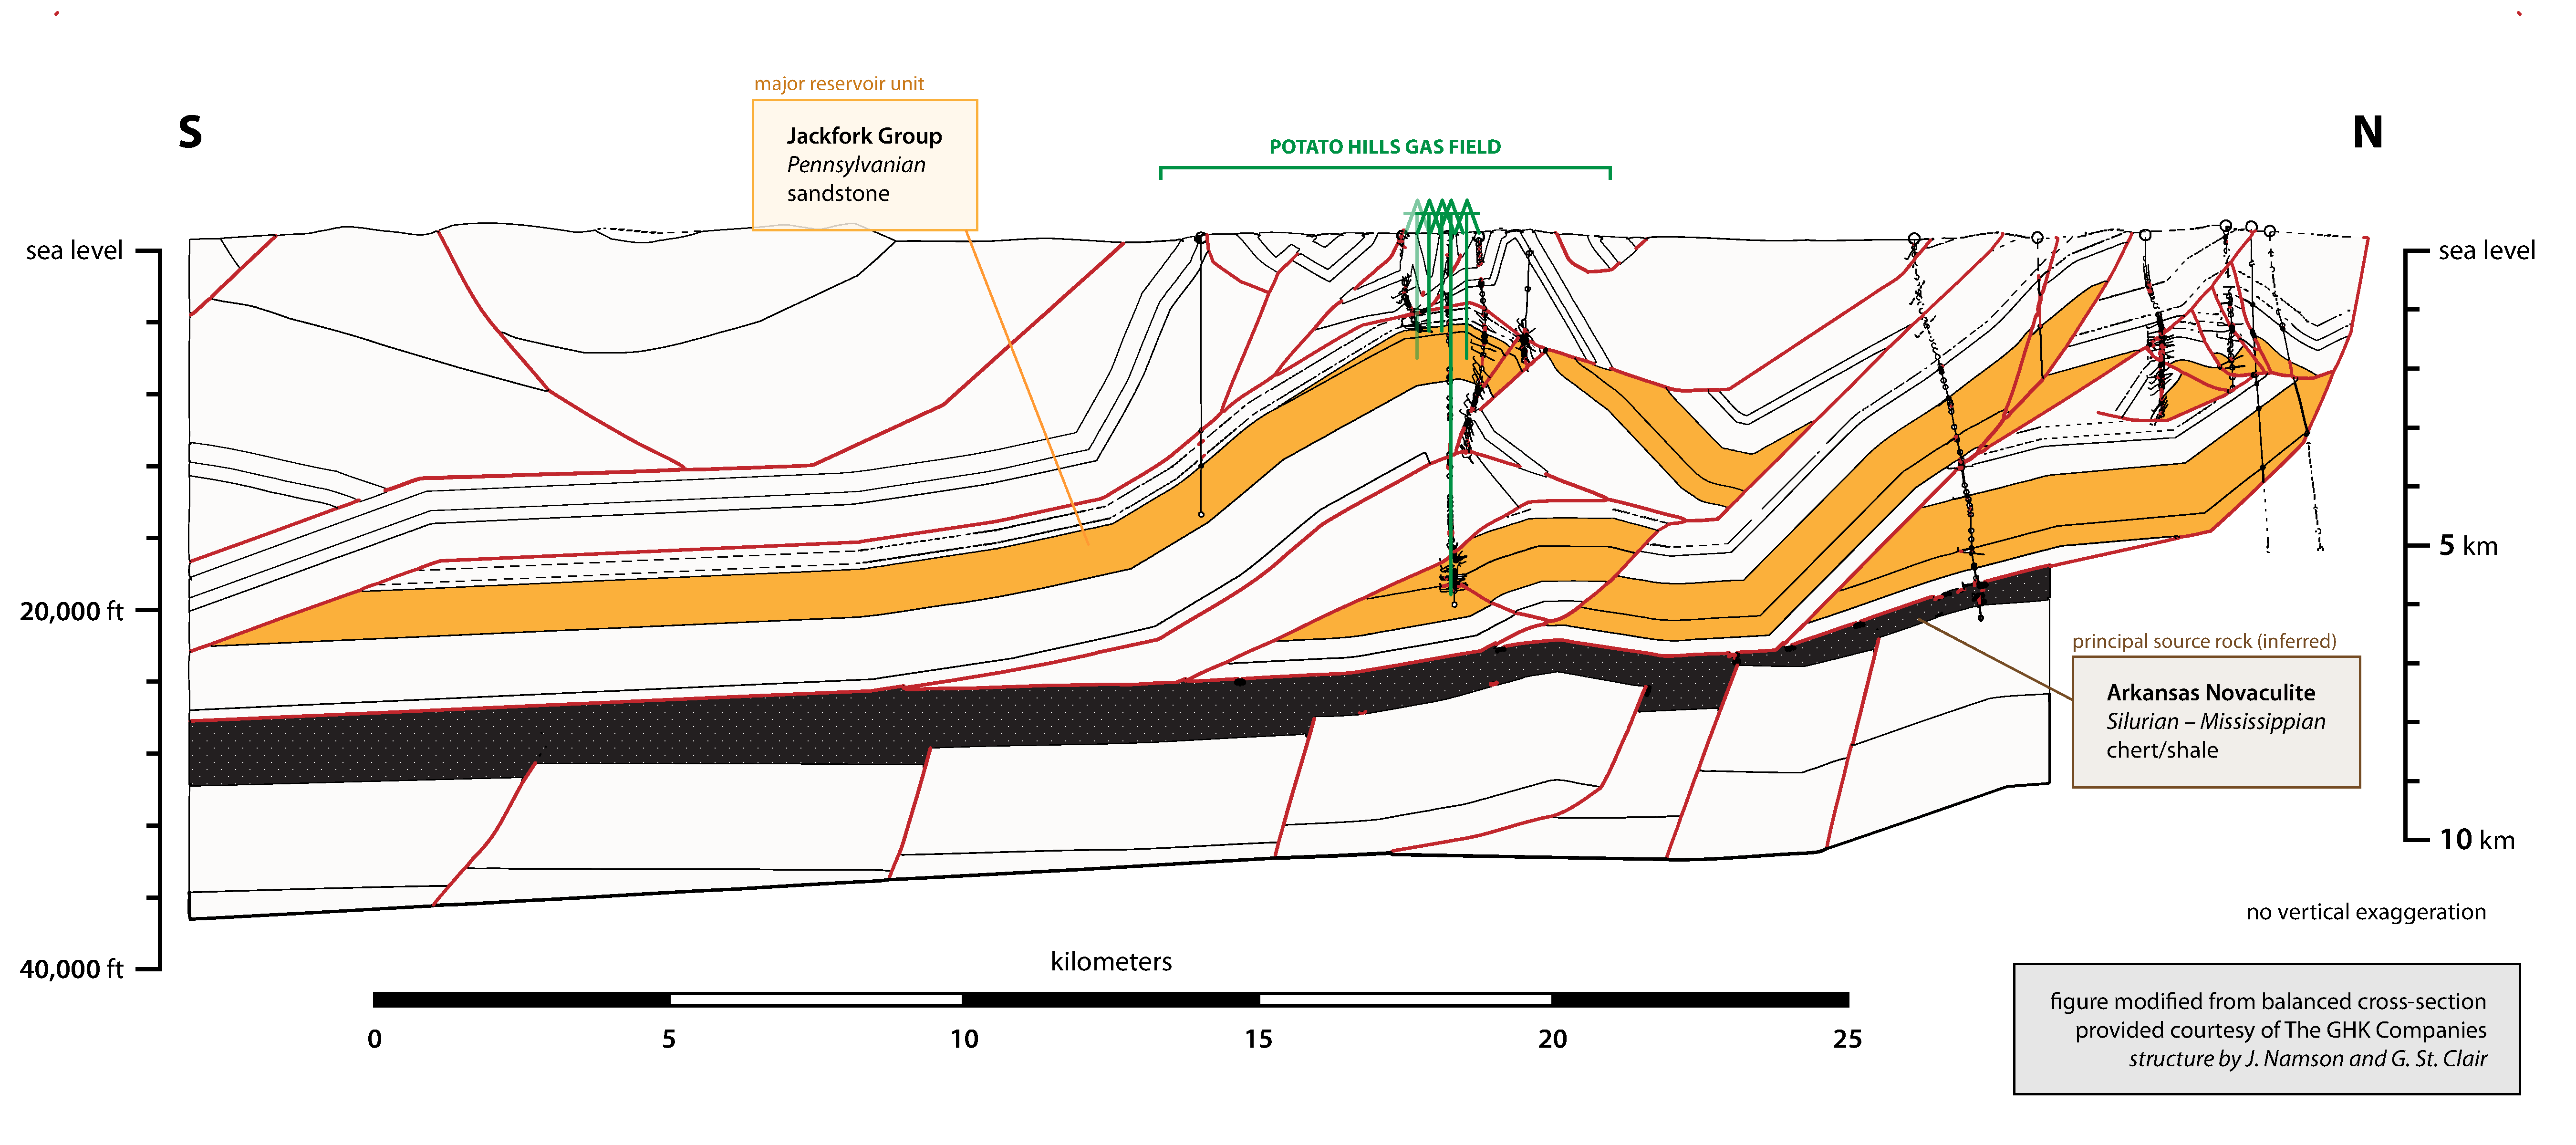
\includegraphics[width=\textwidth]{figures/FigA.2.pdf}
	\caption[Structural cross-section through the Potato Hills]{Balanced geologic cross-section through the Potato
		Hills for A--A$'$ (\autoref{fig:A:1}). The original cross-section on which this figure
		is based was provided courtesy of The GHK Companies. Structural
		interpretation was by J. Namson and G. St.\ Clair. Reservoir sands and
		presumed source are highlighted in orange and black, respectively.
		Faults are highlighted in red. Projections of studied wells onto the
		cross-section are shown in green.}
	\label{fig:A:2}
\end{sidewaysfigure}

The subject of this study is produced gas sampled from the Potato Hills
gas field in southeastern Oklahoma. The Potato Hills is located in a
structurally complex region of the Ouachita Mountains within the
frontal/central thrust belt (\autoref{fig:A:1}).\footnote{The name is apparently
	due to the resemblance of the unevenly-eroded outcrops of the
	fractured Bigfork Chert (late Ordovician) to the knobby mounds of a
	potato garden:
	\url{http://www.ghkco.com/contact/index.php?page=Potato\_Hills}} Wells in
the Potato Hills gas field produce from repeated (subthrusted) intervals
of the fractured and porous sandstones of the Pennsylvanian-age Jackfork
Group (\autoref{fig:A:2}). The field was discovered in the 1960s, but produced little gas and was soon abandoned. Several decades later, The GHK Companies realized the Jackfork play concept and established several
dozen wells in the area beginning in 1997. The Potato Hills is one of
the most significant recent conventional gas discoveries in Oklahoma
\parencite{Boyd_2005_OKGN}, and has produced \textgreater{}300 BCF
(\textasciitilde{}50 MMBOE) of gas.

Major tectonism and mountain building coincided with the collision of
the South American Plate with the North American continent (Laurentia)
during the late Pennsylvanian and early Permian (ca.\ 300~Ma, the
Ouachita orogeny) \parencite{Hatcher++_1989}. During the approach and leadup
to the eventual collision, large deposits of Silurian to
Mississippian-age sediments derived from North American rivers filled
the ocean basin between the two continents. In the Ouachitas, these
sediments are known as the Arkansas Novaculite, an organic-rich (up to
4\% TOC in drill cores, and possibly up to 15\% originally), mixed
shale-chert unit.\footnote{The perhaps more familiar Woodford Shale (to the
north of the Ouachitas, in the Arkoma Basin) is syndepositional to the
Arkansas Novaculite. The Arkansas Novaculite is the basinward extension
of the Woodford Fm.\ \parencite{Houseknecht++_2014_AAPGB}.} While no data from
source rocks in the Potato Hills could be located, the Arkansas
Novaculite elsewhere in the Ouachitas contains predominantly gas-prone
Type III kerogen \parencite{Curiale_1981_thesis}.

Gases from the Potato Hills are dry (\textgreater{}95\%
C\textsubscript{1}/$\big\sum\!$C\textsubscript{1--4}) and express a
partially-reversed isotopic trend in which the CH\textsubscript{4} is
enriched in \textsuperscript{13}C and D relative to C\textsubscript{2}
and higher hydrocarbon gases \parencite{Seewald+Whelan_2005_AAPG-Origin-of-Petroleum}. This partial
reversal is observed in all wells studied, with the exception of the
deep (6.3~km) Mary 2-34 well which produces gases with reversed
δ\textsuperscript{13}C but normal δD (i.e., δD of CH\textsubscript{4}
\textless{} δD of C\textsubscript{2}) (Seewald and Whelan, unpublished
data). Notably, the δD signature of CH\textsubscript{4} is highly
uniform amongst all studied gases (see \autoref{tab:A:1} for a partial listing),
including the deep well.

These gases were studied for two reasons: (\emph{i}) they were samples
of opportunity that were associated with an already-existing dataset
comprising analyses of the chemical and isotopic composition of produced
gases, concentrations of aliphatic acids in coproduced formation waters,
and cultivation-based and culture-independent microbiological data
(Seewald, Whelan, and Sievert, unpublished data); and (\emph{ii}) to
test if migrated thermogenic gases that accumulated in low temperature
reservoir units and were retained over timescales of millions of years
would record primary clumped isotopologue signals.

\section{Methods}\label{methods-2}

\subsection{Samples}\label{samples}

Samples were retrieved from a dusty Pelican case underneath a desk in
Fye 142A at the Woods Hole Oceanographic Institution in October of 2013.

The studied samples were collected from the wellhead in the early 2000's
by GHK in stainless steel cylinders equipped with high-pressure valves,
and furnished to J.\ Seewald and J.\ Whelan for chemical and isotopic
analyses. Data on carbon and hydrogen isotopes of CH\textsubscript{4}
obtained circa 2003 at WHOI \parencite{Seewald+Whelan_2005_AAPG-Origin-of-Petroleum} are shown in
\autoref{tab:A:1}.

There was no evidence of compromised sample integrity when the samples
were examined in 2013--2014. All gas cylinders studied contained gas at
high pressure, and analyses of δ\textsuperscript{13}C and δD in 2014
yielded data that matched those obtained ten years earlier (\autoref{tab:A:1}).

One sample (Mary 2-34) was later mistakenly shipped to UCLA, where it resided for a year.  The missing sample was located and returned to MIT with the help of I.E. Kohl.  All samples are now safely back at WHOI.

\subsection{Analysis}\label{analysis}


\begin{figure*}
	\centering
	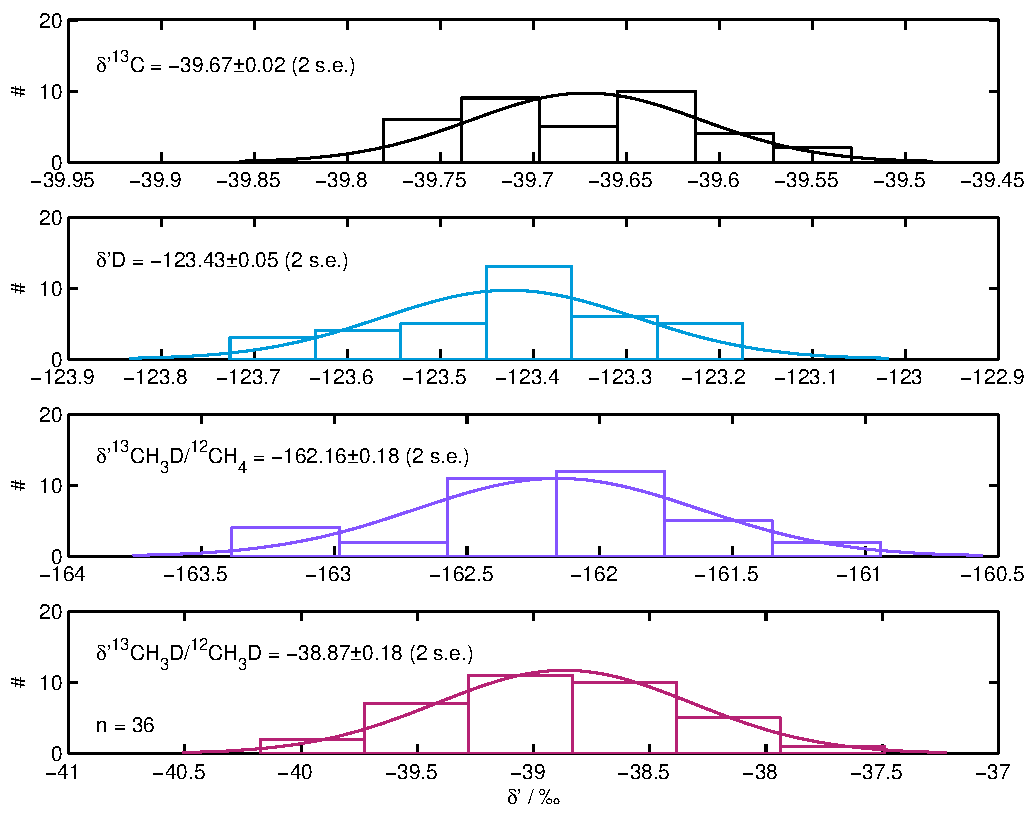
\includegraphics[width=0.85\textwidth]{figures/FigA.3.pdf}
	\captionsetup{format=myformat}	% hrule beneath caption
	\caption[Histogram of isotopologue ratios from a single measurement run]{Histogram of log-delta values (referenced to an
		arbitrary set of isotopologue ratios) for CH\textsubscript{4} purified
		from the Hicks \#1 cylinder, measured on the TILDAS during a single
		sample run (\textasciitilde{}10 hours). Here, \emph{n} represents the
		number of measurement cycles made during this run; in each measurement
		cycle, samples are measured for 100 seconds, and each sample measurement
		is bracketed by measurements on the reference gas.}
	\label{fig:A:3}
\end{figure*}


These samples were the first ``real'' samples ever measured for clumped
isotopologues of methane at MIT. At the time these data were obtained,
the Methane PrepLine (\autoref{dx:C}) had not yet been built, so sample
purification was done manually in a cryogenic vacuum line interfaced
with a gas chromatograph supplied with helium carrier and a handmade
packed column held near ambient temperature.

Analyses of the methane clumped isotopologue
\textsuperscript{13}CH\textsubscript{3}D were made with a prototype
tunable infrared laser direct absorption spectrometer (TILDAS) developed
by Aerodyne Research, Inc.\ (Billerica, MA) and housed in the Hardcore
Stable Isotope Laboratory at MIT. Analytical procedures are documented
in \textcite{Ono++_2014_AC}. A histogram of isotopologue data obtained on
multiple measurement cycles (\emph{n} = 36) for one sample is shown in
\autoref{fig:A:3}.


\section{Results \& Discussion}\label{results-discussion}

\subsection{Preservation potential of clumped isotopologue
	temperatures in migrated thermogenic
	gases}\label{preservation-potential-of-clumped-isotopologue-temperatures-in-migrated-thermogenic-gases}


\begin{table}
	\caption[Isotopic composition of methane from the Potato Hills
	gas field]{Isotopic composition of methane from the Potato Hills
		gas field. Data taken at WHOI soon after sampling \parencite{Seewald+Whelan_2005_AAPG-Origin-of-Petroleum} are compared with data obtained on the same cylinders measured at
		MIT (via TILDAS) one decade later.  All isotope values are in permil (‰).}
	\label{tab:A:1}
	\centering
	\begin{threeparttable}
		\begin{tabular}{l c c cc l ccc c}
			\toprule
			& & & \multicolumn{2}{c}{WHOI (c.\ 2003)} & & \multicolumn{3}{c}{MIT (January 2014)}\tabularnewline
			\cmidrule{4-5} \cmidrule{7-9}
			Well Name & TD (km) & \emph{T}\textsubscript{res} (°C) &
			δ\textsuperscript{13}C & δD & & δ\textsuperscript{13}C & δD &
			Δ\textsuperscript{13}CH\textsubscript{3}D\,\textsuperscript{a} &
			\emph{N}\tabularnewline
			\midrule
			Cedar Creek & 1.78 & 45 & $-$38.1 & $-$134 & & $-$38.4 & $-$136.8 & 3.10 ± 0.25 &
			2\tabularnewline
			Stevens \#1 & 1.86 & 50 & $-$36.9 & $-$139 & & $-$38.1 & $-$136.6 & 3.08 ± 0.37 &
			3\tabularnewline
			Hicks \#1 & 2.29 & 51 & $-$37.0 & $-$135 & & $-$38.2 & $-$136.8 & 3.17 ± 0.20 &
			3\tabularnewline
			Koopmans \#1 & 2.20 & 53 & $-$39.5 & $-$133 & & $-$40.9 & $-$135.3 & 3.30 ± 0.12 &
			5\tabularnewline
			Mary 2-34 & 6.29 & 126 & $-$31.2 & $-$136 & & $-$32.5 & $-$139.7 & 2.94 ± 0.20 &
			5\tabularnewline
			\bottomrule
		\end{tabular}
		{\small TD, total depth; \emph{T}\textsubscript{res}, reservoir temperature; and
		\emph{N}, number of independent replicate purifications and
		measurements.}
		\begin{tablenotes}
			\item[a] The uncertainty on the
			Δ\textsuperscript{13}CH\textsubscript{3}D incorporates propagated 95\%
			confidence intervals calculated assuming a normal distribution, and also
			includes the error on Δ\textsuperscript{13}CH\textsubscript{3}D of AL1.
		\end{tablenotes}
	\end{threeparttable}
\end{table}


Drilled depths and measured reservoir temperatures shown in \autoref{tab:A:1} were
obtained from public records on the website of the Oklahoma Corporation
Commission. Comparison of bottom-hole temperatures to depth for 16 wells
in this area (data from GHK, not shown) suggests a local geothermal
gradient between 15 and 25~°C per kilometer, consistent with the
reported reservoir temperatures and known depths of those reservoir
intervals (\autoref{fig:A:2}).

The Δ\textsuperscript{13}CH\textsubscript{3}D values of gases from all
wells were identical within error, although the deeper Mary 2-34 sample
may carry a slightly lower value (by \textasciitilde{}0.2‰). Samples
yielded geologically-realistic apparent equilibrium temperatures of
\textasciitilde{}150 ± 30~°C (\autoref{fig:A:4}).

To test if these signals might be primary (i.e., if
Δ\textsuperscript{13}CH\textsubscript{3}D values are the same as those
these gases had at the time of their expulsion from the source rock), we
modeled the kinetics of hydrogen isotopic exchange (\autoref{fig:A:4}). This model
uses the rate of CH\textsubscript{4}--H\textsubscript{2}O isotopic
exchange reported by \textcite{Koepp_1978}, and assumes that rates scale with
temperature according to the Arrhenius equation. These rates are subject
to large uncertainty; this is discussed in more depth in \autoref{ch:3} and
in reviews by \textcite{Schimmelmann++_2006_AREarth,Sessions++_2004_GCA}.
Furthermore, the model assumes that
Δ\textsuperscript{13}CH\textsubscript{3}D values will not reset unless
CH\textsubscript{4} exchanges with H\textsubscript{2}O---that is,
homogenous isotope exchange is implicitly excluded as a mechanism for
isotopologue reordering. It is unknown if mineral surfaces encountered
by the hydrocarbons may serve as catalysts for homogenous isotope
exchange \parencite{Shipp++_2014_PNAS}; this would lower the activation energy
and allow isotopic reordering at lower temperatures than indicated.


\begin{figure*}
	\centering
	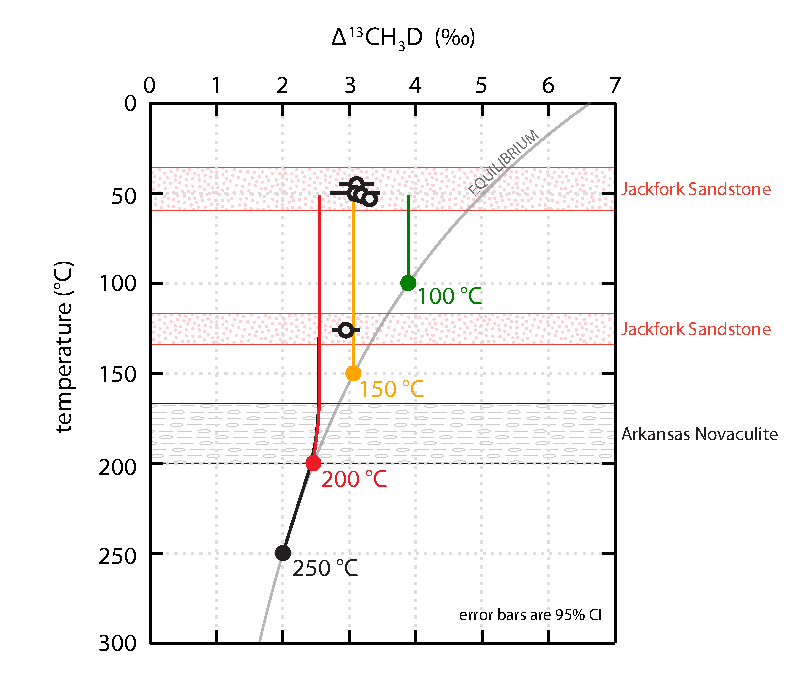
\includegraphics[width=0.9\textwidth]{figures/FigA.4.pdf}
%	\captionsetup{format=myformat}	% hrule beneath caption
	\caption[Cooling model for migrated gases at Potato Hills]{Model of migrating gases. The colored points on the
		model curves represent initial compositions of natural gases that were
		generated at 350~Ma at temperatures from 100 to 250~°C. The gases were
		assumed to be carrying Δ\textsuperscript{13}CH\textsubscript{3}D values
		equal to those expected for equilibrium at these starting temperatures.
		These model gases then were cooled at a rate of 10~°C per Myr until 330~Ma, at which cooling ceased. Curves show the predicted clumped
		isotopologue compositions of gases (\emph{x}-axis) with temperature (\emph{y}-axis).
		Clumped isotopologue reordering was treated as a first-order reaction
		obeying the Arrhenius equation, with pre-exponential factor
		\SI{6.1e9}{\second^{-1}} and activation energy
		209 kJ mol\textsuperscript{$-$1} \parencite[estimated from the data of][]{Koepp_1978}. Data from \autoref{tab:A:1} are shown for comparison. The equilibrium
		curve is that of \textcite{Wang++_2015_S}, for which the equation is listed in
		\autoref{dx:C} (\autoref{eqn:C:equilibrium}).}
	\label{fig:A:4}
\end{figure*}


Migration from source to reservoir is generally thought to be fast
relative to the process of petroleum generation in the source rock
\parencite{England++_1991_AAPG-SV}. A conservative estimate of rates of cooling
during fluid migration was applied (10~°C per Myr). The model results
suggest that isotopic reordering of C--H bonds within
CH\textsubscript{4} is sluggish or non-detectable on timescales relevant
to petroleum migration at temperatures below 200~°C (\autoref{fig:A:4}). This
suggests that if methane generation occurred in the source rocks at
\textless{}200~°C, the signature the methane carried at generation would
have been preserved during its residence in the shallower traps. The
deeper traps may have exceeded this temperature, however (see \autoref{c-h-isotopes-and-the-filling-or-fate-of-fluids-in-the-potato-hills-reservoirs}).
The uniformity of δD but variation in δ\textsuperscript{13}C with depth
indicates that hydrogen exchange has occurred, either by
CH\textsubscript{4}--H\textsubscript{2}O directly, or more likely,
between precursor kerogen and water \parencite{Clayton_2003_IMOG}. Supporting this is
evidence that the Arkansas Novaculite in wells in the vicinity of the
Potato Hills may have reached very high maturities (vitrinite
reflectance \textgreater{}4\% R\textsubscript{o}) \parencite{Guthrie++_1986_AAPGB}.

\subsection{C \& H isotopes and the filling or fate of fluids in the
	Potato Hills
	reservoirs}\label{c-h-isotopes-and-the-filling-or-fate-of-fluids-in-the-potato-hills-reservoirs}

With the exception of the deep well (Mary 2-34), all
δ\textsuperscript{13}C values for methane are quite homogeneous at
around $-$38‰. The methane from Mary 2-34 is characterized by a distinctly
\textsuperscript{13}C-enriched value of $-$32‰, whereas δD is nearly
identical to those of the wells which produce from the shallower
reservoir interval.

Because δ\textsuperscript{13}C values of methane tend to increase with
increasing thermal maturity \parencite{Hunt_1996}, the marked
\textsuperscript{13}C-enrichment in the Mary 2-34 sample suggests that
the deeper reservoir interval was filled by gases that were, on average,
generated at higher temperatures or at a later stage than the gases
which accumulated and were retained in the shallower structural traps.
Several scenarios are possible: (\emph{i}) the shallower trap filled
first, followed later by charging of the deeper trap by more mature
gases; (\emph{ii}) charging of the deeper trap occurred first with enough gas to
fill the deeper reservoir, and spilled over such that the shallower
unit received a vicarious, \textsuperscript{13}C-depleted charge; or 
(\emph{iii}) C\textsubscript{2+} gases in the deeper reservoir have
experienced thermal breakdown or stepwise oxidation such that the
originally \textsuperscript{13}C-depleted signature of
CH\textsubscript{4} has been diluted by heavier carbon-isotope signals
derived from C\textsubscript{2+}.

Interpretations of mapped and extrapolated fault geometries suggest that
thrusting in the frontal and central thrust belts of the Ouachitas
occurred in a break-forward style \parencite{Miser_1929_OGS,Cemen++_2002}.
This implies that crustal shortening, accommodated by development of the
imbricate thrust sheet, was characterized by the formation of new
thrusts underneath older thrusts as the units in the hanging wall moved
forward along the detachment \parencite{Boyer+Elliott_1982_AAPGB,Shaw++_1999_GSAB}. If break-forward thrusting was responsible for the development of
the structural traps of the Potato Hills field, the first scenario may
well be possible.

No information is available to evaluate the second scenario
(fill-to-spill and tertiary migration).

The third scenario is supported by observations of high concentrations
(tens of millimolar) of acetic acid in reservoirs of the Potato Hills
field (Seewald and Whelan, unpublished data). Such high concentrations
of short-chain carboxylic acids are not atypical of oilfield waters
\parencite{Kharaka++_1973_GCA,Willey++_1975_GCA,Carothers+Kharaka_1978_AAPGB,Seewald_2003_N}, and may reflect stepwise oxidation of
C\textsubscript{2+} alkanes to carboxylic acids during residence of the
hydrocarbon fluids in the deep reservoirs \parencite{Shock_1988_G,Seewald_2001_GCA_model}.
Considering that temperatures in the lower reservoir exceed 120~°C
currently, and were likely much higher in the past given that several
kilometers of overburden may have eroded since the Permian \parencite{Godo++_2011_AAPG-ACE}, decomposition of C\textsubscript{2+} alkanes at depth may also
explain features of the isotopic reversals observed \parencite{Burruss+Laughrey_2010_OG,Tilley++_2011_AAPGB,Zumberge++_2012_MPG,Tilley+Muehlenbachs_2013_CG}.

\section*{Acknowledgments}

I thank Jeff Seewald for sharing his samples and data. The GHK Companies
provided much of the background data, the funding for visits to the
producing wells by J. Seewald, J. Whelan, and S. Sievert, and support
for analyses performed at WHOI in the early 2000s. My studies on the
Potato Hills were conducted while under the support of the NDSEG
Fellowship program.









	\chapter{Incorporation of water-derived hydrogen into
	methane during artificial maturation of kerogen under hydrothermal
	conditions}\label{dx:B}
\chaptermark{Kerogen + D\textsubscript{2}O experiment}



\begin{abstract}

	\noindent To investigate the origin of H in hydrocarbons, particularly methane, we
	reacted a sample of organic-rich Eagle Ford shale with
	D\textsubscript{2}O under hydrothermal conditions in a flexible Au-Ti
	cell hydrothermal apparatus in a water:rock ratio of approximately 5:1.
	Temperatures were increased from 200 to 350~°C over the course of one
	month, maintaining pressure at 350 bar, and the concentrations of
	aqueous species and methane isotopologues produced were quantified.
	Production of H\textsubscript{2}, CO\textsubscript{2}, alkanes, and
	alkenes was observed. Methane formed during the early stages of the
	experiment at 200~°C was primarily CH\textsubscript{4} with some
	CH\textsubscript{3}D, whereas at higher temperatures, increasing
	proportions of deuterated isotopologues were produced, such that near
	the end of the experiment, the concentration of CD\textsubscript{4}
	exceeded that of all other isotopologues combined. These results suggest
	that competition between rates of kerogen-water isotopic exchange and
	natural gas generation may govern the D/H ratio of thermogenic gases.

\end{abstract}

\vspace*{\fill}

\noindent \rule{\textwidth}{0.4pt}\\

{\small
	
	\noindent This appendix contains preliminary results from experimental work
	conducted in collaboration with Jeff Seewald, Eoghan Reeves, and Sean
	Sylva at WHOI with input from Shuhei Ono. \\
	
}

\clearpage


\section{Introduction}\label{introduction-4}

Controls on δD values of thermogenic natural gases are often attributed
to kinetically-controlled fractionation during pyrolysis of kerogen or
oils. There are now several studies which have investigated D/H ratios
of methane and other hydrocarbons as a function of maturity \parencite{Sackett_1978_GCA,Berner++_1995_CG,Sackett+Conkright_1997_GCA,Tang++_2005_GCA,Ni++_2011_GCA}. However, kinetic isotope
effects involving hydrogen addition or abstraction are often large and
by themselves do not explain the geologically-reasonable apparent
equilibrium temperatures of \textasciitilde{}150 to 220~°C obtained for
reservoir gases that have been studied for their clumped isotopologue
compositions \parencite{Stolper++_2014_S,Stolper++_2015_GCA,Wang++_2015_S,Young++_2017_GCA}. There is also evidence that δD values of
CH\textsubscript{4} approach values expected for isotopic equilibrium
between CH\textsubscript{4} and H\textsubscript{2}O in formation waters
at temperatures characterizing reservoirs and/or source rocks
(\textasciitilde{}150 to 250~°C) \parencite{Clayton_2003_IMOG,Wang++_2015_S},
although findings of insignificant hydrogen exchange occurring under
these conditions also exist \parencite{Yeh+Epstein_1981_GCA}. In order for
methane samples to have approached or attained equilibrium values of
Δ\textsuperscript{13}CH\textsubscript{3}D and
Δ\textsuperscript{12}CH\textsubscript{2}D\textsubscript{2}, there must
be a pathway by which either (\emph{i}) isotopes can be exchanged
amongst methane isotopologues alone, (\emph{ii}) methane isotopologues
exchange hydrogen with water or organic molecules, or (\emph{iii})
methane isotopologues are derived from methyl moieties which contain
C--H bonds that have pre-exchanged with water prior to forming methane
\parencite{Hoering_1984_OG,Smith++_1985_OG,Schimmelmann++_1999_GCA,Lis++_2006_OG,Schimmelmann++_2006_AREarth}.

Here, we study the origin of C--H bonds in thermogenic methane by
heating kerogen in the presence of D\textsubscript{2}O, and examining
the degree of deuteration in the generated methane. This experiment is
conceptually very similar to those conducted by \textcite{Hoering_1984_OG,Lewan_1997_GCA,Schimmelmann++_2001_OG}. However, none of these workers
quantified the extent of deuteration in the produced natural gases,
though \textcite{Lewan_1997_GCA} mentioned that methane formed in his experiments
contained deuterium.

\section{Methods}\label{methods-3}

\subsection{Experimental methods}\label{experimental-methods}

Experiments were conducted in a gold-titanium reaction cell housed
within a flexible cell hydrothermal apparatus \parencite{Seyfried++_1987} at
WHOI. The reaction cell was pre-treated prior to loading by an overnight
soak in acid.

A sample of Eagle Ford shale from Uvalde County, Texas, USA was used as the source material for this
experiment. The sample was kindly provided to J. Seewald by Keith F. M. Thompson (PetroSurveys, Inc.), and
was powdered to \textless{}\SI{250}{\micro\meter} and Soxhlet-extracted (by Carl Johnson, WHOI).  After extraction, the rock contained about 11\% total carbon, about half of which is acid-dissolvable carbonate (\autoref{tab:B:EA}). The reaction cell was loaded with 10.03 grams of the Soxhlet-extracted powder.  

The starting fluid in Experiment EF-D2O-1 (``DIPPIE-1'') was heavy water
(D\textsubscript{2}O, 99\% purity, Cambridge Isotope Laboratories, Inc.) containing some NaCl (0.497~mol/kg). The added NaCl allows for detection of dilution of the fluid by deionized water from
the pressure vessel in the case of a leak in the reaction cell. The reaction cell was loaded with 55.03~g of this starting fluid.

\begin{SCtable*}
	\centering
	\caption[Elemental analysis of Eagle Ford shale]{Elemental analysis of Eagle Ford shale powder that was either untreated (UNEX), Soxhlet-extracted (EX), or extracted + decarbonated (DECA).  Data from C.~Johnson, WHOI, 1996.} \label{tab:B:EA}
	\begin{threeparttable}
		\begin{tabular}{c d{3} d{3} d{3}}
			\toprule
			(wt\%)	& \multicolumn{1}{c}{UNEX} & \multicolumn{1}{c}{EX*} & \multicolumn{1}{c}{DECA} \\
			\midrule
			C & 12.1  & 11.0 & 6.23 \\
			H & 0.38  & 0.25 & 1.24 \\
			N & 0.18  & 0.17 & 0.74 \\
			S & 0.37  & \textless\!\!0.2 & 2.3  \\
			\bottomrule
		\end{tabular}
		\begin{tablenotes}
			\item * Used in the experiment.
		\end{tablenotes}
	\end{threeparttable}
\end{SCtable*}


\subsection{Analytical methods}\label{analytical-methods}

To monitor the fluid composition and the extent of deuteration, samples
aliquots of fluid were withdrawn through the capillary exit tube into
gastight glass/PTFE syringes. Immediately prior to a sampling event, a
small amount (\textasciitilde{}0.5 g) of fluid was removed and discarded
in order to flush the exit tube of any residues.

The concentration of molecular hydrogen (H\textsubscript{2}) was
determined after headspace extraction using a gas chromatograph supplied
with nitrogen carrier gas, and equipped with a molecular sieve 5Å column
and thermal conductivity detector. Analytical reproducibility of
H\textsubscript{2} data is ±10\% or better (2\emph{s}), however,
accuracy of reported concentrations is currently unknown, because the
relative response of H\textsubscript{2} and D\textsubscript{2} (likely
to be the main form of molecular hydrogen) in the GC-TCD has not yet
been determined. Residual liquid after headspace extraction was diluted
with MilliQ water and saved for analysis of major cations and anions, or
stored with dichloromethane in the fridge in a screw capped vial for
analysis of non-volatile organic compounds.

Concentrations of total dissolved inorganic carbon
($\big\sum\!$CO\textsubscript{2}) and C\textsubscript{1} to C\textsubscript{6}
alkanes and alkenes were determined using a purge-and-trap cryofocusing
device coupled to a gas chromatograph equipped with a Porapak Q column
and serially-connected thermal conductivity and flame ionization
detectors. Analytical procedures were as described in \textcite{Reeves++_2012_GCA}}. Analytical reproducibility on duplicate samples was ±5\% or
better (2\emph{s}). The C\textsubscript{5} and C\textsubscript{6}
compounds could not be quantified accurately due to their semi-volatile
nature; however, C\textsubscript{5} and C\textsubscript{6} were detected
at all sampling points.

At each sampling, a separate \textasciitilde{}1 to 2~ml aliquot was
injected directly into a pre-weighed, evacuated serum vial capped with
boiled blue butyl rubber stoppers, for analysis of the extent of
deuteration of methane. A Hewlett-Packard (HP) 6890 gas chromatography-mass
spectrometry (GC-MS) system equipped with a 5Å molecular sieve column (HP-PLOT 30 m $\times$ 0.32 mm $\times$ \SI{12.0}{\micro\meter}) and HP 5973 mass selective detector was
used to determine the amount of deuteration in CH\textsubscript{4}. Ion
currents were monitored at integral masses between \emph{m}/\emph{z} 10 and 50. Extracted ion currents were quantified at \emph{m}/\emph{z} 14 through 23 for methane.  Expected fragmentation patterns of each of the methane-\emph{d} isotopologues were determined by analysis of commercial synthetic standards (\textgreater{}98\% purity, Cambridge Isotope Laboratories, Inc.).

\section{Results \& Discussion}\label{results-discussion-1}

\subsection{Concentrations of aqueous
	species}\label{concentrations-of-aqueous-species}


\begin{sidewaysfigure}
	\centering
	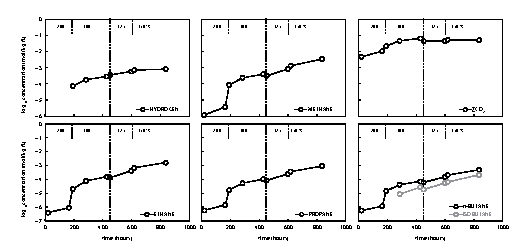
\includegraphics[width=\textwidth]{figures/FigB.1}
	\caption[Concentrations of aqueous species during experiment EF-D2O-1.]{Concentrations of aqueous species during experiment EF-D2O-1.  Note the log scale for concentration.}
	\label{fig:B:1}
\end{sidewaysfigure}

\begin{sidewaysfigure}
	\centering
	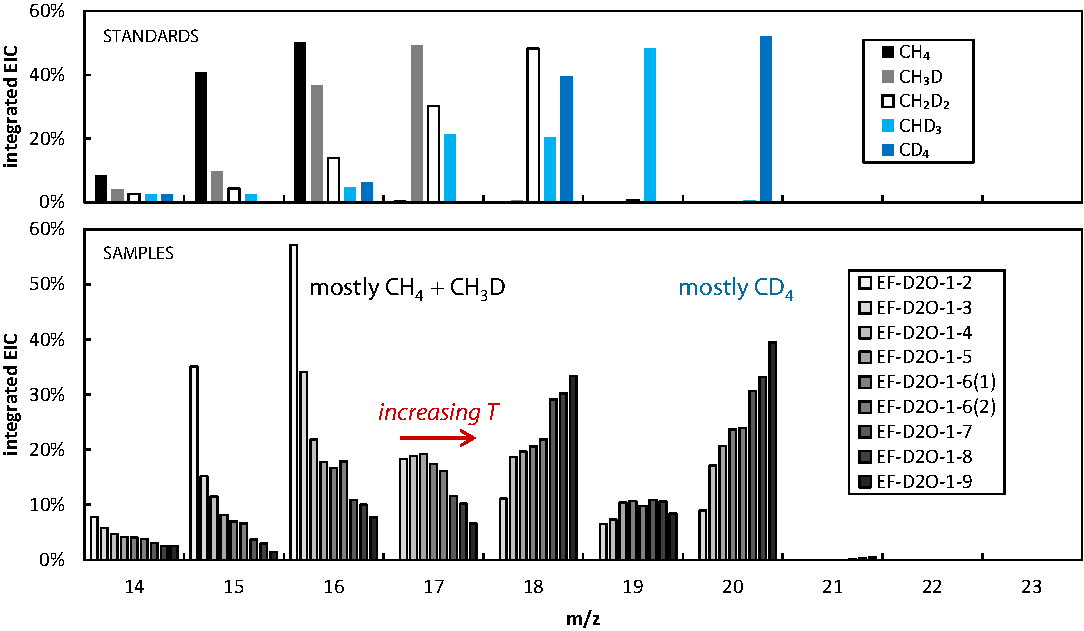
\includegraphics[width=0.85\linewidth]{figures/FigB.2}
	\caption[Mass spectra of methane generated in experiment EF-D2O-1]{Mass spectra of methane generated from artificial maturation of Eagle Ford shale in the presence of D\textsubscript{2}O.}
	\label{fig:B:2}
\end{sidewaysfigure}

\begin{SCfigure*}
	\centering
	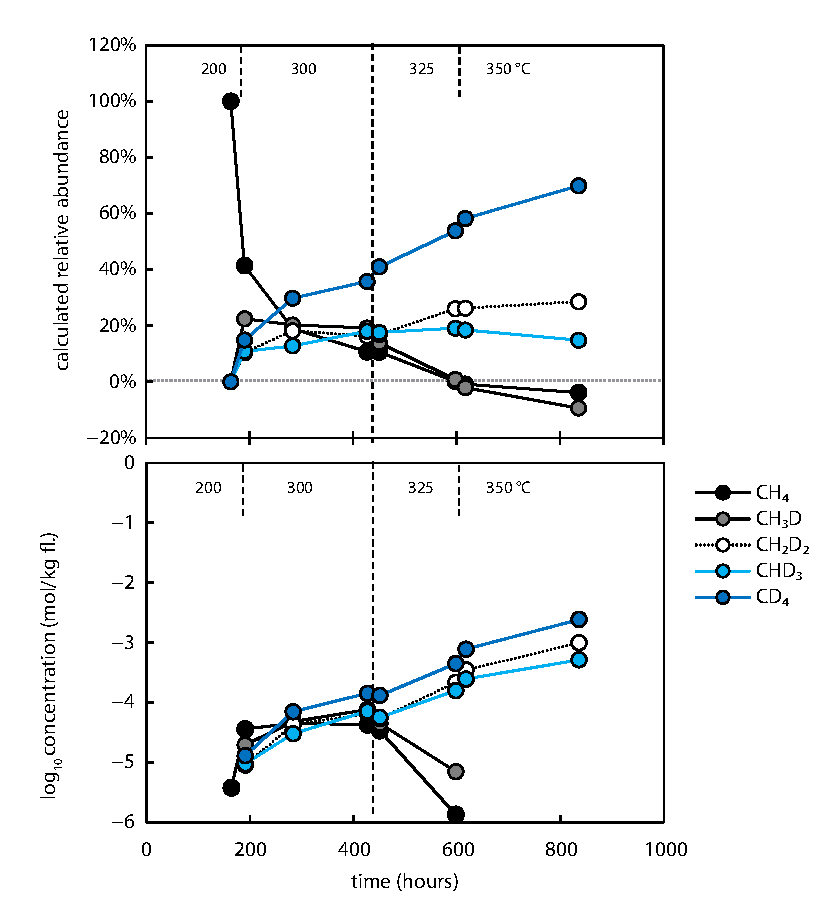
\includegraphics[width=0.75\linewidth]{figures/FigB.3}
	\caption[Estimated relative and absolute abundances of methane
	isotopologues in experiment EF-D2O-1]{Estimated relative and absolute abundances of methane
		isotopologues. Concentrations less than zero are an artifact of
		uncertainty in standardization and may potentially be corrected by
		applying algorithms to account for contributions of fragment ions to
		peaks in the lower range of \emph{m}/\emph{z}. Note the log scale on the \emph{y}-axis in the
		bottom panel.}
	\label{fig:B:3}
\end{SCfigure*}
\begin{table*}
	\centering
	\caption[Concentration of aqueous species during Experiment	EF-D2O-1]{Concentration of aqueous species during Experiment EF-D2O-1, heating of Soxhlet-extracted Eagle Ford shale at 200 to 350~°C	and 350~bar in the presence of saline D\textsubscript{2}O fluid.}
	\label{tab:B:1}
	\begin{threeparttable}
		\begin{tabular}{c c ccc c c}
			\toprule
			Sample	& Time 	& \ce{H2} 	& \ce{CH4}	&  $\big\sum\!$\ce{CO2} 	& \multirow{2}{*}{C\textsubscript{1}/C\textsubscript{2--4}}	& pD\\%\tnote{a} \\ 
			\# 		&  (h)	& (µmol/kg) & (µmol/kg) & (mmol/kg)	& & (25~°C)\\
			\midrule
			\multicolumn{7}{l}{\emph{Experiment begun with 52.6 g fluid at temperature of 200~°C}}\\
			1 &	19	& BDL (\textless{}10) &	1.2	& 4.8 &	0.11&\\	
			2 &	164	& BDL (\textless{}10) &	3.8 &	10.8 &	0.37&\\	
			\multicolumn{7}{l}{\emph{Temperature raised to 300~°C}}\tabularnewline
			3 &	191	& 773 &	87	& 21.9 &	1.00	&\\
			4 &	284	& 183 &	235	& 45.8 &	0.86	&\\
			5 &	427	& 290 &	396	& 65.5 &	0.86	&\\
			\multicolumn{7}{l}{\emph{Injected \textasciitilde{}18.3 g starting fluid and raised temperature to 325~°C}}\tabularnewline
			6 &	451	& 353 &	319	& 44.7 &	0.89	&\\
			7 &	598 & 586 &	825	& 45.3 &	0.85	&\\
			\multicolumn{7}{l}{\emph{Raised temperature to 350~°C}}\tabularnewline
			8 &	617	& 718 &	$ 1.32\times10^3 $ &	54.4 &	0.89 &	\\
			9 &	836	& 821 &	$ 3.47\times10^3 $ &	51.2 &	1.00 &	5.90\\
			\bottomrule
		\end{tabular}
	
		\begin{tablenotes}
			\item[a] The listed pD value was calculated from pH measured
			with a glass electrode: pD = pH\textsubscript{measured} + 0.41 \parencite{Glasoe+Long_1960_JPC}.
		\end{tablenotes}
	\end{threeparttable}
\end{table*}
%\multirow{2}{*}{C\textsubscript{1}/C\textsubscript{2--4}}

%\begin{table}
%	\begin{tabular}{c c c}
%		AAA & 1 & 22\\
%		BBB & 2 & 33\\
%	\end{tabular}
%\end{table}

Measured concentrations of aqueous species are shown in \autoref{fig:B:1}.
Concentrations of H\textsubscript{2} increased from undetectable
(\textless{}10~µmol/kg) to up to 0.8~mmol/kg at the end of the
experiment. Increasing concentrations of H\textsubscript{2} within
temperature stages of the experiment suggests that generation of
petroleum, as opposed to a mineral redox buffer, is influencing the
H\textsubscript{2} concentration. H\textsubscript{2} increased much more
slowly during the \textgreater{}300~°C stages compared to heating at 300~°C and below.

The concentration of $\big\sum\!$CO\textsubscript{2} increased during the early
stages of the experiment, and leveled off at \textasciitilde{}50~mmol/kg
at 350~°C. This might indicate that carbonate reached saturation and began to precipitate
\parencite{Seewald++_1998_GCA}; to verify this, measurements of major cations
are required. Production of CO\textsubscript{2} as the most abundant
product of hydrothermal alteration of kerogen is also consistent with
prior experimental work \parencite{Seewald_2003_N}. Alternatively, carbonate could have been released from the rock as it had not been decalcified prior to heating. 

Concentrations of methane
increased at all time steps, as did concentrations of detected
\emph{n}-alkanes. Except for the beginning of the experiment, molar
concentrations of C\textsubscript{1} and $\big\sum\!$C\textsubscript{2--4} were
very similar and increased in near lock step.

\subsection{Production of deuterated
	methane}\label{production-of-deuterated-methane}



The relative abundance of methane-\emph{d} isotopologues was quantified by GC-MS
for all samples except the one from timepoint \#1, for which no methane
peaks of usable size could be obtained (\autoref{fig:B:2}).

Methane formed during the early stages of the experiment at 200~°C was
primarily CH\textsubscript{4} with some CH\textsubscript{3}D, whereas at
higher temperatures, the isotopologues produced consist almost
exclusively of CD\textsubscript{4}, CH\textsubscript{3}D, and
CH\textsubscript{2}D\textsubscript{2} (\autoref{fig:B:3}). These results suggest
that at relatively lower temperatures of \textasciitilde{}200~°C, the
rate of methane generation approaches or exceeds the rate of D/H
exchange between water and kerogen, whereas at higher temperatures,
extensive D/H exchange between kerogen (or oils, if they are also
precursors of methane) and water occurs prior to methane generation.
CD\textsubscript{4} became the dominant methane species at temperatures
of 300~°C and above, suggesting that more than 50\% of all labile,
methane-generating sites on kerogen were fully deuterated.
Alternatively, the dominance of CD\textsubscript{4} might be explained
by direct CH\textsubscript{4}--H\textsubscript{2}O isotopic exchange
occurring after the generation of primarily non-deuterated methane. This
is unlikely given the sluggish pace at which D/H exchange occurs for
methane \parencite{Reeves++_2012_GCA}. Experiments in which normal water is
heated in the presence of CD\textsubscript{4} while the D/H of water is
monitored may yield a more sensitive determination of the exchange rate
constant for CH\textsubscript{4}--H\textsubscript{2}O.

Production of CH\textsubscript{4} at the beginning of the experimenst
indicates that the ``capping'' hydrogen was derived from kerogen or
other H-containing species in the rock as opposed to water.
Alternatively, the CH\textsubscript{4} observed at the first time point
may have been sorbed to a solid phase and leached into the fluid.
Production of CH\textsubscript{4} and CH\textsubscript{3}D appeared to
cease by midway through the 300~°C stage. Continued (though relatively
minor) production of methane that was not fully-deuterated
(CHD\textsubscript{3} and CH\textsubscript{2}D\textsubscript{2}, \autoref{fig:B:3},
bottom panel) suggests that kerogen or oil from which methane was
generated did not fully exchange before methane formed.

While examining the total ion and extracted ion chromatograms to
quantify the deuteration in CH\textsubscript{4}, an unknown and
unexpected peak was found eluting immediately following the
CH\textsubscript{4} and air peaks. This mystery peak appeared to yield
methyl fragments that were also progressively more deuterated with
reaction time. Re-analysis of several samples while scanning a higher
mass range suggested that the mystery compound had stable fragments near
\emph{m}/\emph{z} 45 to 50 (depending on degree of deuterium
substitution). This was verified by GC-MS analysis of a commercial
isobutane standard (mostly isobutane-\textit{d}\textsubscript{0}) which yielded a
base peak at \emph{m}/\emph{z} 43. No attempt to quantify the degree of
deuteration in isobutane was made.

\section{Acknowledgments}\label{acknowledgments-4}

Financial support for this work was provided by a Shell-MITEI Fellowship
and by NSF award EAR-1250394 to S. Ono.





	\chapter{Additional methodological details, data, and \\site
	descriptions}\label{dx:C}
\chaptermark{Additional methods and site descriptions}

This section provides additional, unpublished information regarding
methods or field observations that support the research presented in
the preceding chapters.

\section{\texorpdfstring{Equilibrium 
		Δ\textsuperscript{13}CH\textsubscript{3}D versus
		temperature}{Calculated equilibrium Δ13CH3D versus temperature}}\label{calculated-equilibrium-ux3b413ch3d-versus-temperature}

\mrefs[B]{Figure}{fig:C:2} shows the calculated values of ln \emph{K}\textsubscript{eq} vs.\ temperature for the reaction:
\begin{equation}\label{eqn:C:exchange}
{}^{13}\text{CH}_4+ {}^{12}{\text{CH}}_3\text{D}\rightleftharpoons {}^{13}{\text{CH}}_3\text{D}+ {}^{12}{\text{CH}}_4 
\end{equation}

\noindent A good fit to the curve is obtained with the expression:
\begin{equation}\label{eqn:C:equilibrium}
1000\ln K = \left( 1.68169 \times 10^{14} \right)\left( \frac{1}{T^{2}} \right)^{3} - \left( 1.40754 \times 10^{10} \right)\left( \frac{1}{T^{2}} \right)^{2} + \left( 6.72697 \times 10^{5} \right)\left( \frac{1}{T^{2}} \right) - 0.28671
\end{equation}
where temperature \emph{T} is in kelvin.


\begin{figure*}
	\centering
	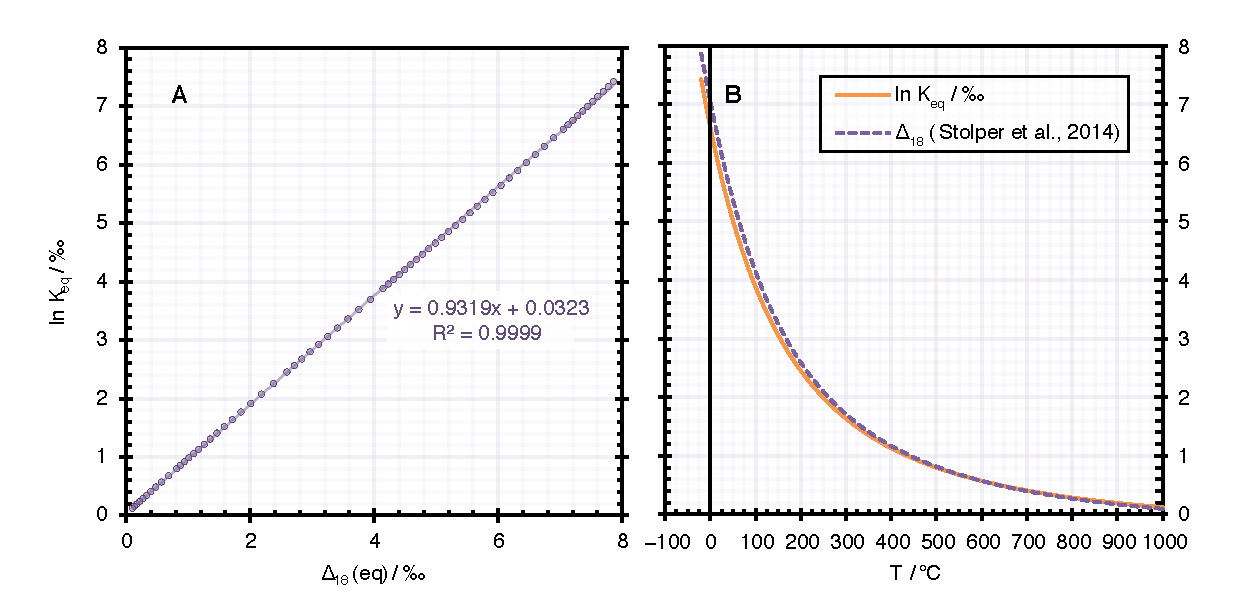
\includegraphics[width=\textwidth]{figures/FigC.2}
	\captionsetup{format=myformat}	% hrule beneath caption
	\caption[Equilibrium Δ\textsubscript{18} and Δ\textsuperscript{13}CH\textsubscript{3}D values as a function of temperature]{Equilibrium Δ vs.\ $T$ curves.  (\textbf{A}) Conversion between equilibrium
		Δ\textsubscript{18} values and equilibrium
		Δ\textsuperscript{13}CH\textsubscript{3}D values. Note that conversion
		of Δ\textsubscript{18} to Δ\textsuperscript{13}CH\textsubscript{3}D can
		only be done if it is known or can be assumed that methane isotopologues
		have attained their equilibrium distribution at the temperature
		indicated by both Δ\textsuperscript{13}CH\textsubscript{3}D and Δ\textsuperscript{12}CH\textsubscript{2}D\textsubscript{2}. Nonequilibrium
		Δ\textsubscript{18} values cannot easily be converted to
		Δ\textsuperscript{13}CH\textsubscript{3}D, particularly if Δ \textless{}
		0 ‰ (anticlumped). (\textbf{B}) Comparison between equilibrium
		Δ\textsuperscript{13}CH\textsubscript{3}D [= ln
		\emph{K}\textsubscript{eq} for the isotope exchange reaction (\autoref{eqn:C:exchange}), defined
		following \textcite{Ono++_2014_AC} and calculated as in \textcite{Wang++_2015_S}], and equilibrium Δ\textsubscript{18}
		values from \textcite{Stolper++_2014_GCA}.}
	\label{fig:C:2}
\end{figure*}

\section{Notes on analytical procedures}

\subsection{\texorpdfstring{Isolation of CH\textsubscript{4} using
		cryofocusing-preparative gas
		chromatography}{Isolation of CH4 using cryofocusing-preparative gas chromatography}}\label{isolation-of-ch4-using-cryofocusing-preparative-gas-chromatography}

\begin{sidewaysfigure}
%	\centering
	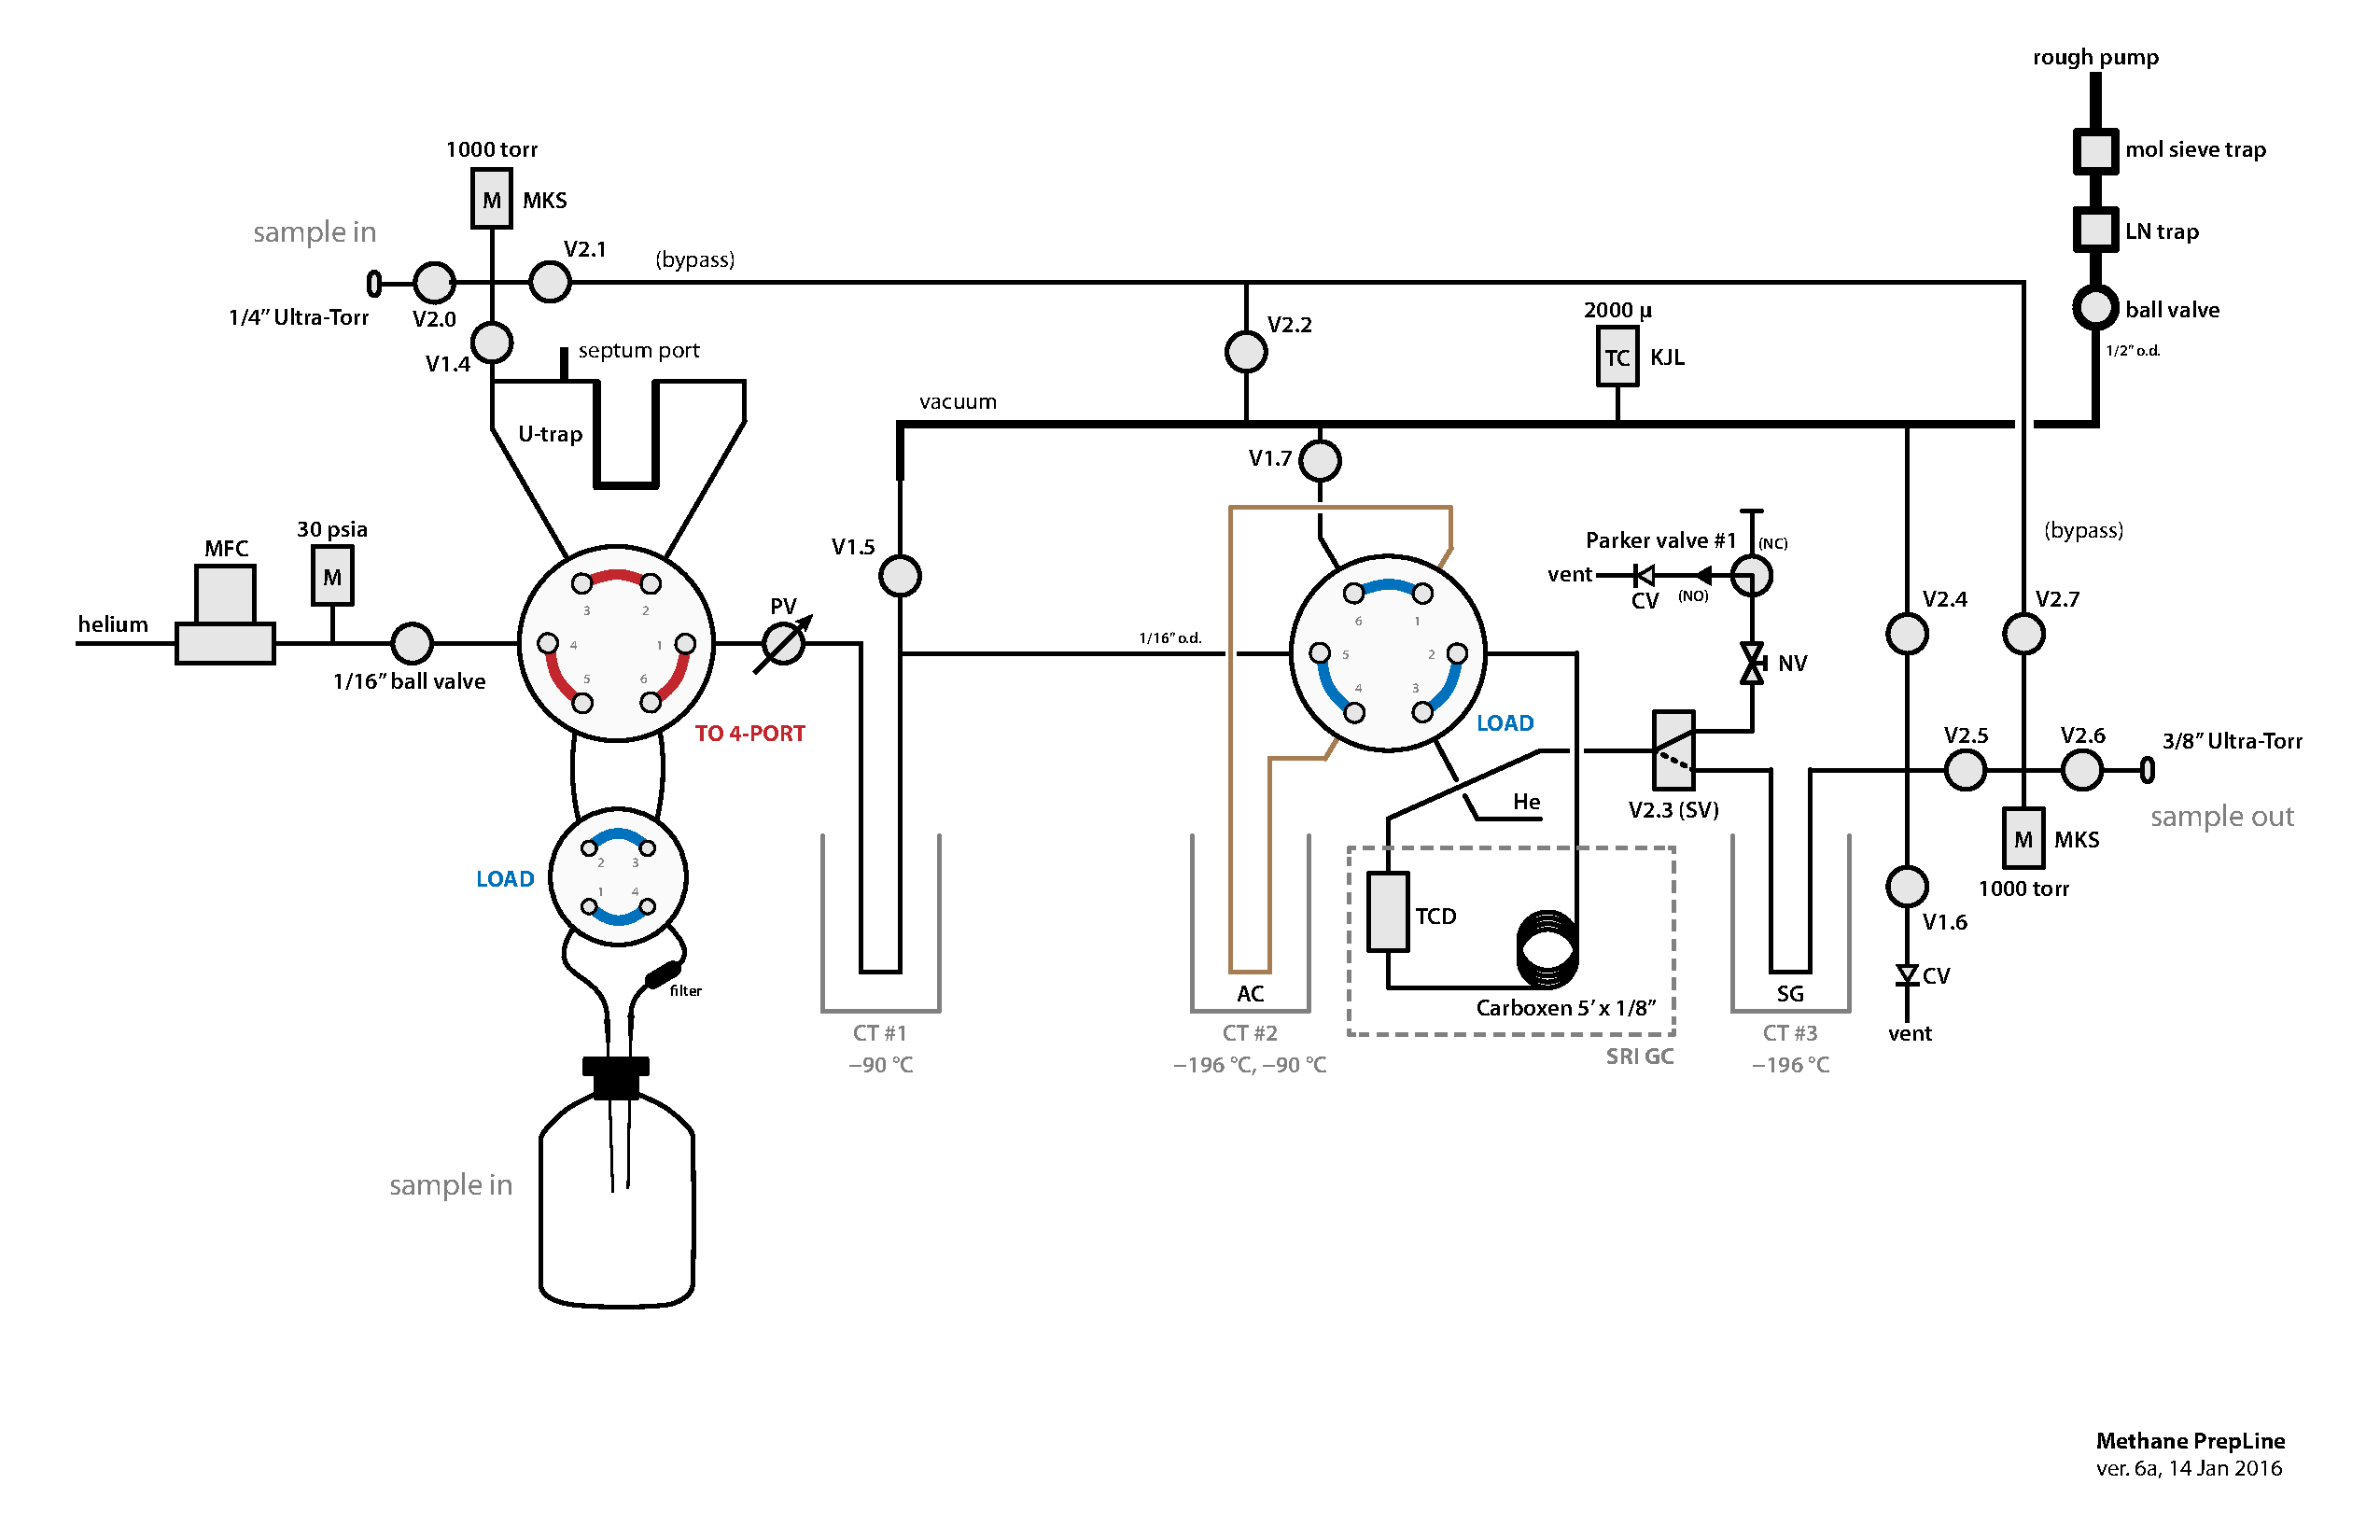
\includegraphics[width=\textwidth]{figures/FigC.1.pdf}
	\caption[Schematic of methane preparation system]{Schematic of methane preparation system at the MIT
		Hardcore Stable Isotope Laboratory.}
	\label{fig:C:1}
\end{sidewaysfigure}


\mrefs[]{Figure}{fig:C:1} shows a schematic of the methane preparation system used to
isolate CH\textsubscript{4} for measurement of
Δ\textsuperscript{13}CH\textsubscript{3}D by TILDAS at MIT from mid-2014
onwards \parencite{Wang++_2015_S,Inagaki++_2015_S,Wang++_2016_GCA,Lopes++_2016_JoDS,Whitehill++_2017_GCA}. The system consists of a
cryotrapping-preparative gas chromatography system interfaced with a
vacuum line and a helium supply. A software interface built using
National Instruments LabVIEW controls all pneumatically- and
electronically-actuated valves, pistons for dewars on cold traps, and
heating coils. Operation is mostly automatic and hands-free.
Preparation time is \textless{}45~minutes for a typical sample of
1--15~cm\textsuperscript{3} SATP CH\textsubscript{4} and
\textless{}200~cm\textsuperscript{3} air. Air blanks in the purified gas
are typically \textless{}0.10~cm\textsuperscript{3} SATP.

The retention time of methane on the PrepLine column depends on the amounts of both \ce{CH4} and ``air'' (\ce{O2}, \ce{Ar}, \ce{N2}, \ce{CO})
in the sample, as shown in \autoref{fig:C:GC}.

\begin{SCfigure*}
	\centering
	\includegraphics[width=0.55\linewidth]{figures/FigC.GC}
	\caption[Dependence of the retention time of \ce{CH4} on volumes of \ce{CH4} and air on the PrepLine]{Dependence of the retention time of \ce{CH4} (\emph{x}-axis) on on-column volumes of \ce{CH4} (\emph{y}-axis) and ``air'' (= \ce{O2} + Ar + \ce{N2} + \ce{CO}) on the Prep\-Line.  The sample is heated off cold trap \#2 and injected onto the column between 15~seconds and 1~minute.  Compounds in order of elution are \ce{H2}, air, \ce{CH4}, and \ce{CO2} + \ce{C_{2+}}.}
	\label{fig:C:GC}
\end{SCfigure*}

\subsection{Correction of non-linearity in isotopologue concentration
	data}\label{correction-of-non-linearity-in-isotopologue-concentration-data-returned-by-tdlwintel}

Data retrieved from TDLWintel (Aerodyne Research, Inc., Billerica, Mass.)\footnote{For a history of the development of TDLWintel for applications with tunable diode and quantum cascade laser instruments, see \textcite{Horii++_1999_SPIE,Zahniser++_1995_PTRSA,Nelson++_2002_ApplPhysB,Nelson++_2004_SA-A}.} are in the form of number
densities (ND) that the software calculates from line parameters in the HITRAN database \parencite{Brown++_2013_JQSRT,Rothman++_2013_JQSRT}. For
all clumped isotopologue data collected in this thesis except those in
\autoref{dx:A}, the following correction scheme was applied.  Isotopologue/isotope ratios reported were calculated from the corrected number densities ($\mathrm{ND}_{6x}^\mathrm{corr}$).  
\begin{equation}\label{eqn:C:correction}
\mathrm{ND}_{6x}^\mathrm{corr} = \mathrm{ND}_{6x}^\mathrm{meas} + D_{6x} \cdot \mathrm{ND}_{61}^\mathrm{meas} + H_{6x} \cdot \mathrm{ND}_{61}^\mathrm{meas} \cdot \left(1 - \frac{\mathrm{ND}_{61}^\mathrm{meas}/P_\mathrm{meas}}{\mathrm{ND}_{61}^\mathrm{pure}/P_\mathrm{target}} \right)~
\end{equation}
Here, $\mathrm{ND}_{6x}^\mathrm{meas}$ are the number densities returned by TDLWintel in the \texttt{STR} files, $P_\mathrm{meas}$ is the pressure of the sample in the cell, $P_\mathrm{target}}$ = \SI{1.0383}{\torr}, and $\mathrm{ND}_{61}^\mathrm{pure}$ (= \num{3.88e6}) is the number density of \ce{^{12}CH4} for a sample of pure methane at the target pressure.  
Calibrated values for the correction factors $D$ and $H$ are listed in \autoref{tab:C:correctionfactors}.  Note that the $D$ and $H$ here are just variable names, and are not related to deuterium or hydrogen.  Numbering of isotopologues is from HITRAN.
\begin{SCtable*}[][bp]
	\centering
	\caption[Correction factors applied to measured number densities]{Correction factors for \autoref{eqn:C:correction}. Values were determined during 2014--2015.  Values for $D$ were derived from measurements of methane heated to equilibrium over a catalyst, and values for $H$ were derived from measurements of methane admixed with different percentages of \ce{N2} in the TILDAS cell.}
	\label{tab:C:correctionfactors}
	\begin{tabular}{clcd{4}}
	\toprule
	\# & isotopologue & $D$ & H\tabularnewline
	\midrule
	61 & \textsuperscript{12}CH\textsubscript{4} & 0 & 0\tabularnewline
	62 & \textsuperscript{13}CH\textsubscript{4} & 0 & -0.0033\tabularnewline
	63 & \textsuperscript{12}CH\textsubscript{3}D & 0 & -0.0036\tabularnewline
	64 & \textsuperscript{13}CH\textsubscript{3}D & \num{3.00e-3} & -0.0125\tabularnewline
	\bottomrule
	\end{tabular}
\end{SCtable*}

I have found this correction scheme to sufficiently correct the observed
non-linearity in δ\textsuperscript{13}CH\textsubscript{3}D vs.\ δ\textsuperscript{12}CH\textsubscript{3}D over a wide range of
δ\textsuperscript{12}CH\textsubscript{3}D values (from $-$600 to +400‰ vs.\ AL1) (the $D$ term), as well as any air that might make its way into the system (up to
10\%) (the $H$ term; the portion enclosed in parentheses represents an estimate of the percentage impurity in the methane sample).\footnote{The $D$ term 
corrects the observation that measured Δ\textsuperscript{13}CH\textsubscript{3}D values are lower than their true values when δD of the sample 
is lower than that of the reference gas (and vice versa).  The $H$ terms correct an observed elevation in all three δ-values when impurities (primarily air) are 
present in the sample (important for the recycling technique used on small samples because air can accumulate in the sample due to small leaks in the TILDAS inlet system).}
Part of the reason for the nonlinearity is that the Voigt profile cannot accurately account for the tailing of one or more large \textsuperscript{12}CH\textsubscript{4} peaks
that are located immediately outside the wavelength region scanned by the laser.

\subsection{Calibration of isotopic composition of in-house standards
	(AL1)}\label{calibration-of-isotopic-composition-of-in-house-standards-al1}

%\input{tables/tableC.2}

The δ\textsuperscript{13}C and δD values we report have been calibrated
relative to PDB and SMOW, respectively, by measuring samples of NGS-1
(also known as NIST SRM 8559 and USGS-A) and NGS-3 (also known as NIST
SRM 8561 and USGS-C), which are natural gas standards with published
reference values for δ\textsuperscript{13}C and δD, as listed in \autoref{reporting-of-ux3b413c-and-ux3b4d-values} \parencite[supplementary materials in][]{Wang++_2015_S}. Samples of these natural gases were
included in a set of calibration samples distributed by the USGS to
various laboratories in the U.S. in July 2014. These samples were
contained in IsoTubes (Isotech Laboratories, Illinois, USA) at pressures
of \textasciitilde{}3 bar. We subsampled aliquots of these gases through
a septum adapter fitting (available from Isotech) using a 25~ml gastight
syringe (SGE Analytical Science), and introduced the aliquots into our
sample preparation system as described above.

Data shown in this thesis for δ\textsuperscript{13}C, δD, and
Δ\textsuperscript{13}CH\textsubscript{3}D assume that reference gas AL1
has the isotopic composition $-$34.5‰, $-$147.7‰, and $+$2.41 ± 0.07‰ (95\% CI)
respectively, consistent with \textcite{Wang++_2015_S} and with the values we
provided to the UCLA group \parencite{Young++_2016_IJMS}.\footnote{The values originally reported in \textcite{Ono++_2014_AC} are quite different in δD (by \textasciitilde{}20‰) for reasons as yet undetermined.  Anecdotal experience suggests that this is probably related to a historical problem of poorly-anchored δD values for GC-IRMS analyses of methane within the isotope community, with resultant differences in calibration between the several IRMS labs from which values for δD
of AL1 vs.\ SMOW were obtained.  I favor the revised values listed above for reasons of consistency with the NGS gases and the new USGS samples.} 

\section{Miscellaneous unpublished information on selected sites}\label{miscellaneous-unpublished-information}

This section contains miscellaneous data and ruminations that do not yet have a proper home in the literature.
\clearpage 

\subsection{\texorpdfstring{Additional field notes and thoughts on selected localities studied by \textcite{Wang++_2015_S}}{Additional field notes and thoughts on selected localities studied by Wang et al.\ (2015)}}\label{field-notes-and-thoughts-on-selected-localities}

\subsubsection{Lower Mystic Lake}\label{lower-mystic-lake}

The water sample from Lower Mystic Lake shown in \autoref{ch:2} was sampled from the water column at a depth of 18 mbll,
which is below the chemocline. It should be noted that the isotopic
composition of pore waters in Lower Mystic Lake sediments, at the
time(s) and depth(s) at which the methane was generated, may be or have
been significantly different than that of the water in the water column.
This is because prior to the implementation of water management
practices, Lower Mystic Lake was tidally-influenced, and the bottom waters were derived from seawater that flowed upriver along the bottom of the Mystic
River. Dams constructed in 1908 and 1966 slowed or stopped the influx of
seawater, and initiated a gradual reduction in the volume of anoxic and
sulfidic bottom waters in the lake; the reduction in bottom waters was
also accelerated by intentional removal of bottom waters by pumping and
treatment in the 1980s and 1990s \parencite{Duval+Ludlam_2001_IRHb,Ludlam+Duval_2001_LRM}. Therefore, even though the δD of Lower Mystic Lake water
at 18 mbll ($-$40.6 ± 1.0‰, 1\emph{s}) was similar to that of Upper Mystic
Lake ($-$39.2 ± 1.8‰, 1\emph{s}), the Lower Mystic Lake sediment pore
waters may have an isotopic signature that is closer to that of seawater
(\textasciitilde{}0‰). This trend is observed in other coastal
meromictic lakes in which seawater is trapped below the chemocline
\parencite{Jeffries++_1984_CJES}. Assuming a value of 0‰ for the associated
waters for methane generated in Lower Mystic Lake sediments would not
affect our conclusions; on the contrary, it would suggest that the field
of primary microbial methane could be constrained even more tightly than
\autoref{fig:2:2} indicates.

\subsubsection{CROMO}\label{cromo}

The water sample from the Coast Range Ophiolite Microbial Observatory (CROMO) for which the δD\textsubscript{water} value
is reported in \autoref{ch:2} was collected from the CSWold well. This well
is noted in publicly-available reports on water quality monitoring in
the area, but we do not presently have information on the depth(s) at
which the groundwater at CSWold is derived. However, the δD value of the
water is consistent with mixing between deep sedimentary-derived brines
and meteoric waters \parencite{Peters_1993_GCA}.

At CROMO, the δ\textsuperscript{13}C and δD data alone cannot
conclusively distinguish between thermogenic, abiogenic, and microbial
origins of the methane. Specifically, the CROMO gases are highly similar
in δ\textsuperscript{13}C and δD to the sample of natural gas from the
Utica Shale (\autoref{tab:2:S1} and \autoref{fig:2:1}), where the gases are
generally inferred to have been generated by thermogenic processes. The
Δ\textsuperscript{13}CH\textsubscript{3}D values at each field site are
very dissimilar, however, with the Utica Fm. gases having an apparent
temperature \textasciitilde{}160~°C and the CROMO gases having apparent
temperatures of 42 to 76~°C. Therefore, the clumped isotopic measurement
provides information that is complementary to, and independent of, the
bulk δ\textsuperscript{13}C and δD data, a conclusion that is not
obvious from previous studies.

I suggest that at CROMO, the isotopic composition of the gases
(δ\textsuperscript{13}C, δD, and
Δ\textsuperscript{13}CH\textsubscript{3}D) is inconsistent with a
significant contribution from thermogenic sources of methane.\footnote{Note that this is somewhat different from what was written by \textcite{Wang++_2015_S}.}
Furthermore, the C\textsubscript{1}/C\textsubscript{2} ratio (measured
using GC-FID) ranged from 360 to 1540 (\autoref{tab:2:S5}) for
samples of dissolved gases collected from 5 wells (including N-, CSW-,
and QV- wells) sampled in July 2014; these
C\textsubscript{1}/C\textsubscript{2} ratios are within the range
expected for microbial gases (\textgreater{}100), and outside the range
of values typically observed for thermogenic gases (\textless{}100).

If the framework presented in \autoref{fig:2:2} is correct, then a major source of
uncertainty in differentiating between the possible processes of methane
generation is the δD of the associated waters from which methane was
produced. Specifically, meteoric water in the vicinity of CROMO
generally has lower δD values ($-$70 to $-$50‰) \parencite{Peters_1993_GCA,Kendall+Coplen_2001_HP} than what was measured for water from the CSWold well
($-$33‰; \autoref{tab:2:S5}). Previous work on natural springs in the
vicinity of the McLaughlin mine suggested that groundwater in this
region can be best characterized as a two-component mixture consisting
of formation brines derived from the Great Valley Sequence mixed with
variable amounts of low-salinity meteoric water \parencite{Peters_1993_GCA}.
Parenthetically, I note that the
Δ\textsuperscript{13}CH\textsubscript{3}D-based temperatures for methane
at CROMO (42 to 76~°C) would suggest isotopic equilibration with water
that has a δD in the range of 0 to +20‰ (\autoref{fig:2:2}). This range is
consistent with the δD value (+11‰) of the most saline waters
({[}Cl\textsuperscript{\textminus}{]} \textasciitilde{} 580 mmol/kg) sampled by
\textcite{Peters_1993_GCA} from springs in the vicinity of CROMO. The apparent
temperatures of 42 to 76~°C for methane at CROMO are within the accepted
temperature limits of life (generally \textless{}80~°C, but up to 122~°C
for hyperthermophilic methanogens). Thus, based on the consistency of
the observed isotopic signatures with other geochemical parameters
(namely, {[}H\textsubscript{2}{]}, \autoref{fig:2:3}), I infer a
dominantly-microbial origin of the methane at CROMO originating from deep groundwater below the ophiolite body. Methanogenesis does not appear to occur to any appreciable extent in the shallow (meteoric) groundwaters.  More recent microbiological work showing a total absence of archaea, including methanogens, from 16S sequences of the CROMO waters  \parencite{Twing++_2017_FMicro} appears to support this conclusion.   

\subsection{Methane isotopologue data on assorted samples}

\begin{table}\centering
	
	\caption[Isotopologue data for assorted methane samples]{Isotopologue data for methane samples from a rice paddy in Sherrill, Arkansas, USA, and the Chimaera seepage, Tekirova ophiolite, Turkey. Uncertainties
		reported are 95\% confidence intervals. Values for
		δ\textsuperscript{13}C, δD, and
		Δ\textsuperscript{13}CH\textsubscript{3}D are reported relative to PDB,
		SMOW, and the stochastic distribution, respectively.}
	\label{tab:C:3}

	\begin{threeparttable}
		
		\begin{tabular}{@{} l l r@{\hspace{0.2em}}l r@{\hspace{0.2em}}l >{\raggedleft\arraybackslash}p{2.5em}@{\hspace{0.2em}}l r@{\hspace{0.2em}}l @{}}
			% This notation >{\raggedleft\arraybackslash}p{5em} is for padding the left side so that multicolumn doesn't expand extra space on the right column of the multicolumn{2}{c}. http://stackoverflow.com/a/25690685
			\toprule
			Site & Sample Name & \multicolumn{2}{c}{δ\textsuperscript{13}C (‰)} & \multicolumn{2}{c}{δD (‰)} &
			\multicolumn{2}{c}{Δ\textsuperscript{13}CH\textsubscript{3}D (‰)} & \multicolumn{2}{c}{\textit{T}\textsubscript{13D}
				(°C)}\tabularnewline
			\midrule
			Sherrill & JTB-1-2 & \textbf{$-$56.40} & ± 0.05  & \textbf{$-$336.47} & ± 0.05  &
			 \textbf{$-$0.47} & ± 0.23  & \textbf{a.c.} &  \tabularnewline
%			\midrule
			Chimaera* & S8\_271949\_4034797\_12.10.2013 & \textbf{$-$11.41} & ± 0.03  & \textbf{$-$119.50} & ± 0.05  &
			\textbf{3.19} & ± 0.18  & \textbf{141} & +13/$-$12 \tabularnewline
			& S4 & \textbf{$-$11.62} & ± 0.10  & \textbf{$-$119.57} & ± 0.10  &
			\textbf{2.62} & ± 0.54  & \textbf{185} & +55/$-$42 \tabularnewline
			& S5 & \textbf{$-$11.37} & ± 0.10  & \textbf{$-$119.42} & ± 0.10  &
			\textbf{2.98} & ± 0.43  & \textbf{156} & +35/$-$29 \tabularnewline
			& S9 & \textbf{$-$11.38} & ± 0.12  & \textbf{$-$119.49} & ± 0.14  &
			\textbf{3.32} & ± 0.34  & \textbf{133} & +23/$-$21 \tabularnewline
			\bottomrule
		\end{tabular}
	
		\begin{tablenotes}
			\item * Samples from Chimaera were measured more than 6 months apart (May to December 2014).  The data appear to be unaffected by storage or instrumental drift over this period.
		\end{tablenotes}
	
	\end{threeparttable}
\end{table}




\subsubsection{Rice paddy, Sherrill, Arkansas, USA}\label{rice-paddy}
A sample of gas was collected by J.T. Bird from a paddy rice field in Sherrill, Arkansas, USA in June of 2014.  Bubbles of gas were released by gentle agitation of the submerged sediment, trapped in a funnel, and transferred to serum bottles containing several milliliters of 1~M NaOH added to inhibit microbial activity.  On the day of collection, air temperature was 93~°F and skies were cloudy.  Given that the daily lows had been steady at 70~°F for five days and the water on the field had been standing for ``a good two weeks'' (Sherrill local, via J.T. Bird, pers.\ comm.), estimated water temperatures are \textasciitilde{}75~°F or about 25~°C.  

Analysis of methane in the sample (\autoref{tab:C:3}) yielded relatively low δ\textsuperscript{13}C and δD values ($-$56‰ and $-$336‰) typical of biologically-produced methane in wetlands.  The Δ\textsuperscript{13}CH\textsubscript{3}D value was anticlumped (ca.\ $-$0.5‰).  This is the lowest degree of \textsuperscript{13}C--D clumping we have observed in any natural methane sample aside from seep gases at The Cedars.  

\subsubsection{Chimaera seep, Tekirova ophiolite, Turkey}
Four samples of gases collected by H.\ Hoşgörmez from the Chimaera seep (Yanartaş, meaning ``flaming rock'', near the Gulf of Antalya, eastern Mediterranean Sea; also the source of the first Olympic flame)   were sent to us by G.\ Etiope.  Samples arrived in glass vessels equipped with gas-tight stopcocks at both ends.  

Analyses of methane in these samples yielded relatively high bulk δ\textsuperscript{13}C and δD values ($-$11‰ and $-$119‰, \autoref{tab:C:3}) consistent with those previously reported for the same site \parencite{Etiope++_2011_EPSL,Hosgormez++_2008_Gf,Hosgormez_2007_JAsES}.  The δ\textsuperscript{13}C values lie outside the typical range of known thermogenic methane (up to $-$20‰), and δD values are close to those required for D/H equilibrium with water of SMOW-like hydrogen-isotope composition at temperatures upwards of ca.\ 200~°C (\autoref{fig:3:5}).  The Δ\textsuperscript{13}CH\textsubscript{3}D data indicated apparent equilibrium temperatures averaging 153~°C.  These temperatures are much higher than the \textless50~°C temperatures at which abiotic methane was inferred by \textcite{Etiope++_2011_EPSL} to be synthesized here.  Recently-published data obtained by the UCLA group on several other samples taken at Chimaera yielded Δ\textsuperscript{13}CH\textsubscript{3}D values (ranging from +3.3 to +3.6‰) in general agreement with ours, as well as Δ\textsuperscript{12}CH\textsubscript{2}D\textsubscript{2} values that are at or near equilibrium at the same temperatures indicated by Δ\textsuperscript{13}CH\textsubscript{3}D \parencite{Young++_2017_GCA}.  These data indicate that methane carrying clumped isotopologue abundances similar to those of typical thermogenic gases probably comprises a large fraction of the Chimaera seep gas and that such gases may contribute more to the seepage flux than was previously suggested.  



\section{Errata and corrigenda to published articles} \label{errata}

The following mistakes have been found in the two articles published from this thesis.
\begin{description}
	\item[\textcite{Wang++_2015_S}]  (\emph{i}) In Figure S4, the arrows denoting secondary isotope fractionation were labeled incorrectly; this is corrected in \autoref{fig:2:S4}.  (\emph{ii}) Several footnotes in Table S3 were incomplete or incorrectly labeled; this is fixed in \autoref{tab:2:S3}.  (\emph{iii}) Samples from the Powder River Basin were misstated as being from Wyoming.  These samples were actually taken from wellheads located in Montana, near the border with Wyoming (API well numbers 25-003-22076, 25-003-22192, and 25-003-22074, in order of appearance in \autoref{tab:2:S1}).  Also, well ``3CA34'' was completed in the Cook Coal as stated in the paper, but produces from the stratigraphically-higher Canyon Coal according to information on the Montana Board of Oil \& Gas Conservation website. \autoref{ch:2} contains the corrected information.  Several typographical errors have also been corrected.
	\item[\textcite{Wang++_2016_GCA}]  In Table 2, citations to the \citeauthor{Joelsson++_2014_CPL} papers were inadvertently switched.  \textcite{Joelsson++_2015_ACPD,Joelsson++_2016_ACP} should be cited for \ce{CH4}~+~OH and \textcite{Joelsson++_2014_CPL} for \ce{CH4}~+~Cl\@.  \autoref{tab:4:2} lists the correct references.
\end{description}



\section{Acknowledgments}
% \addcontentsline{toc}{section}{Acknowledgments}

Shuhei Ono and Bill Olszewski provided key assistance with the design, 
construction, and troubleshooting of the Methane PrepLine.  Kyle Delwiche and Genming Luo are thanked for their help in the field at Lower Mystic Lake, and for insightful conversations.  Discussions with Matt Schrenk, Billy Brazelton, Katrina Twing, Mike Kubo, and Tori Hoehler helped form my views on the CROMO gases.  Dan Ritter provided the information regarding locations of wells in the Powder River Basin.  Jordan Bird graciously went out of his way to sample the Arkansas rice paddy (and take video footage!).  Giuseppe Etiope is thanked for sending us the samples from the Chimaera seep.






	
%	\nocite{*}

%\DeclareNameAlias{default}{last-first}
	
	\backmatter
	\defbibnote{myprenote}{%{\scshape \textcolor{myred}{note}} \; 
		\color{myred} \itshape \small Numbers listed in parentheses at the end of citations %\emph{(\textcolor{myred}{red})} 
		refer to pages on which the work was cited.}
	\renewcommand*{\bibfont}{\small}
%	\printbibliography[prenote=myprenote,title=References]

%\assignrefcontextentries[sorting=nyt]{*}
	\begin{refcontext}[sorting=nyt]%,maxalphanames=1,labelalpha,maxbibnames=99]
%	\raggedright
	\printbibliography[prenote=myprenote,title=References]
	\end{refcontext}

	\cleartoevenpage
	
	\figureversion{osf}
	\thispagestyle{empty}
	\vspace*{0.3\textheight}
	
	\noindent \textsw{\bfseries The Geochemistry of Methane Isotopologues}\\
	
	\vspace{12pt}
	
	\noindent \textsc{David T. Wang}  \raisebox{-5pt}{\includegraphics[height=14pt]{figures/DTWcc}}
	
	\vspace{6pt}
	
	\noindent {\itshape E-mail}: \href{mailto:dtw@alum.mit.edu}{\nolinkurl{dtw@alum.mit.edu}}\\
	{\textsc{orcid}}: \noindent\href{http://orcid.org/0000-0002-2656-8951}{\nolinkurl{0000-0002-2656-8951}}\\
	
	\vspace{12pt}
	
	\noindent Submitted \nth{5} May 2017\\
	\noindent\textit{Cambridge, Massachusetts}\\
	
	\vspace*{\fill}
	
	\noindent {Prepared using \LaTeX{}.}
	
	
	
\end{document}



